%%%%%%%%%%%%%%%%%%%%%%%%%%%%%%%%%%%%%%%%%
% Stylish Article
% LaTeX Template
% Version 2.1 (1/10/15)
%
% This template has been downloaded from:
% http://www.LaTeXTemplates.com
%
% Original author:
% Mathias Legrand (legrand.mathias@gmail.com) 
% With extensive modifications by:
% Vel (vel@latextemplates.com)
%
% License:
% CC BY-NC-SA 3.0 (http://creativecommons.org/licenses/by-nc-sa/3.0/)
%
%%%%%%%%%%%%%%%%%%%%%%%%%%%%%%%%%%%%%%%%%

%----------------------------------------------------------------------
%	PACKAGES AND OTHER DOCUMENT CONFIGURATIONS
%----------------------------------------------------------------------

\documentclass[fleqn,10pt,twoside]{SelfArx} % Document font size and equations flushed left

\usepackage[english]{babel} % Specify a different language here - english by default

\usepackage{lipsum} % Required to insert dummy text. To be removed otherwise
\usepackage{todonotes} % Lets me add the many many todos that still need to be done

% Group together figures with separate captions
\usepackage{caption}
\usepackage{subcaption}

% Coloured boxes to make things pretty
\usepackage{tcolorbox}
\usepackage{graphicx}

% Huxtable compatability
\usepackage{threeparttable}
\usepackage{adjustbox}
\usepackage{hhline}
\usepackage{colortbl}

% Multiline support in tables
\usepackage{multirow}
% This allows us to have centred fixed width columns in tables
\newcolumntype{P}[1]{>{\centering\arraybackslash}p{#1}}
\newcolumntype{M}[1]{>{\centering\arraybackslash}m{#1}}

% For multiple columm itemize lists
\usepackage{multicol}


%----------------------------------------------------------------------
%	COLUMNS
%----------------------------------------------------------------------

\setlength{\columnsep}{0.8cm} % Distance between the two columns of text
\setlength{\fboxrule}{0.75pt} % Width of the border around the abstract
\setlength{\columnseprule}{0.5pt}

%----------------------------------------------------------------------
%	COLORS
%----------------------------------------------------------------------

\definecolor{color1}{RGB}{0,0,90} % Color of the article title and sections
\definecolor{color2}{RGB}{0,20,20} % Color of the boxes behind the abstract and headings
\definecolor{boxcolour}{HTML}{CCDFFF} % Colour of my arbitrary boxes

%----------------------------------------------------------------------
%	HYPERLINKS
%----------------------------------------------------------------------

\usepackage{hyperref} % Required for hyperlinks
\hypersetup{hidelinks,colorlinks,breaklinks=true,urlcolor=color2,citecolor=color1,linkcolor=color1,bookmarksopen=false,pdftitle={Title},pdfauthor={Author}}

% ----- GET FIGURES AND TABLES TO BEHAVE ------%
\usepackage{float}

%----------------------------------------------------------------------
%	ARTICLE INFORMATION
%----------------------------------------------------------------------

\JournalInfo{West Sussex County Council} % Journal information
\Archive{June 2022} % Additional notes (e.g. copyright, DOI, review/research article)

\PaperTitle{West Sussex JSNA Summary 2021/22} % Article title

\Authors{Public Health and Social Research Unit}%, James Smith\textsuperscript{2}} % Authors
\affiliation{\textsuperscript{1}\textit{Public Health and Social Research Unit, West Sussex County Council, West Sussex, United Kingdom}} % Author affiliation
%\affiliation{\textsuperscript{2}\textit{Department of Chemistry, University of Examples, London, United Kingdom}} % Author affiliation
\affiliation{*\textbf{For more information, please contact}: Matthew.Dorey@westsussex.gov.uk} % Corresponding author

\Keywords{Covid-19 --- Mental Health --- Service Planning --- Population Health Management --- Health Equity} % Keywords - if you don't want any simply remove all the text between the curly brackets
\newcommand{\keywordname}{Keywords} % Defines the keywords heading name


%----------------------------------------------------------------------
%	ABSTRACT
%----------------------------------------------------------------------

\Abstract{The West Sussex Joint Strategic Needs Assessment (JSNA) sets out the health and wellbeing needs of the population of West Sussex. It is not a single document or piece of analysis but encompasses a range of work, including detailed needs assessments relating to specific subjects or communities, evaluations of new programmes or activities, local surveys, and a range of briefings and ad hoc analyses. This summary is a brief run-through of the data available.}

%----------------------------------------------------------------------
\begin{document}
\renewcommand{\abstractname}{What is a JSNA?} % Makes the abstract title something more akin to what we would expect
\flushbottom % Makes all text pages the same height

\maketitle % Print the title and abstract box

\tableofcontents % Print the contents section
%\listoftodos
\thispagestyle{empty} % Removes page numbering from the first page

%----------------------------------------------------------------------------------------
%	ARTICLE CONTENTS
%----------------------------------------------------------------------------------------
\paragraph{Contacts and Further Information} This report was drafted by the West Sussex Public Health and Social Research Team with support from colleagues from across the council and local organisations.

% For further information please contact:
% \begin{itemize}[noitemsep]
% \item jacqueline.clay@westsussex.gov.uk
% \item catherine.wells@westsussex.gov.uk
% \end{itemize}

% Specific analysts for individual life stages are provided at the end of each section.

\paragraph{JSNA Website} We place full reports, information and links on the West Sussex JSNA website. \url{https://jsna.westsussex.gov.uk/}

\paragraph{Posters available} We are keen to disseminate the information from the JSNA. For some subjects we have drafted posters which can be downloaded from the website.

\paragraph{West Sussex Life} The current version of West Sussex Life can be found on the West Sussex website. (\url{https://www.westsussex.gov.uk/campaigns/west-sussex-life/})

% \paragraph{CIPFA Neighbours} The current CIPFA comparable local authorities for West Sussex are: Cambridgeshire, Devon, East Sussex, Essex, Gloucestershire, Hampshire, Kent, North Yorkshire, Northamptonshire, Oxfordshire, Somerset, Staffordshire, Suffolk, Warwickshire, Worcestershire.

% information on CIPFA neighbours and how to read data to go in appendix - but might also be able to create some text boxes

\setlength{\parindent}{0cm}
\setlength{\parskip}{1em}
\newpage
\section{Introduction} % The \section*{} command stops section numbering

%\addcontentsline{toc}{section}{Context} % Adds this section to the table of contents
\begin{tcolorbox}[width=\linewidth, colback={boxcolour}]
    \subsection{What is a JSNA?}
    The West Sussex Joint Strategic Needs Assessment (JSNA) sets out the health and wellbeing needs of the population of West Sussex. It is not a single document or piece of analysis but encompasses a range of work, including detailed needs assessments relating to specific subjects or communities, evaluations of new programmes or activities, local surveys, and a range of briefings and ad hoc analyses. {\bf This summary is a brief run-through of the data available.}
\end{tcolorbox}

\paragraph{Scale, Direction and Significance}
Being presented with a lot of facts and figures can be overwhelming. We recommend keeping three things in mind when assessing quantitative data:
\begin{itemize}
    \item Develop a clear understanding of the {\bfseries SCALE} of an issue in understanding population level needs. {\textit For example, in West Sussex there are approximately 160-200 teenage pregnancies in a year.}
    \item Look at the trend or {\bfseries DIRECTION} - if you have a good time series of data, look at the short, medium and long term. {\textit For example, in relation to teenage pregnancy, there is a long downward trend locally and nationally.}
    \item Finally, look at {\bfseries SIGNIFICANCE} - is one year different to the next, or one place compared with another? In this summary we use the term significant to mean \textit{statistically} significant (meaning a difference that isn't due to random chance). \textit{For example, locally there was a rise in teenage pregnancy between 2016 and 2017 but this was small and not significant.}
\end{itemize}

\begin{tcolorbox}[title={CIPFA Neighbours}, colback={boxcolour}]
Data in this summary are compared in a number of ways: over time, between different groups in the population, or by area. We frequently compare information with England and with "comparable local authorities". The Chartered Institute of Public Finance and Accounting (CIPFA) group local authorities by looking at population characteristics (such as population, socioeconomic indicators, household and mortality characteristics).

For West Sussex our current (January 2020) comparable authorities are:
\small
\begin{multicols}{3}
\begin{itemize}
    \item Cambridgeshire
    \item Devon
    \item East Sussex
    \item Essex
    \item Gloucestershire
    \item Hampshire
    \item Kent
    \item North Yorkshire
    \item Northamptonshire
    \item Oxfordshire
    \item Somerset
    \item Staffordshire
    \item Suffolk
    \item Warwickshire
    \item Worcestershire
\end{itemize}
\end{multicols}
\end{tcolorbox}

% \subsection{What's new in the 2021/22 JSNA Summary?}
% \todo[inline]{Given the time now available I might not go through with all these threatened rearrangements of structure}Since the previous West Sussex JSNA Summary (2019/20, available here), Covid-19 has had a profound impact on health care and public health in West Sussex and beyond. Covid-19 at time of writing continues to be a global pandemic with huge implications for public health provision at all levels: locally, nationally and internationally.

% In the years ahead Covid may well change the definition of public health services and what can be expected from them. This is not only because of the disease itself, but also the disruptions to other services that have occurred due to lockdowns and other interventions, and the need to provide additional services to support efforts against covid. 

% As a result, this JSNA summary needs to consider that impact and act as a guide for how and where services need to react to this new world that we live in. At time of writing, it is not known whether the post-Covid world is one in which the disease is all but eliminated or whether it becomes an endemic disease that we must live with. This document aims to support commissioners of services in either eventuality. 

% Previous summaries in West Sussex have structured the document around the life course, broadly grouping topics according to whether they sit with children and young people (starting well), working age adults (living well) and older adults later on in life (ageing well). However, given the need for urgent action in many areas across the life course this chronological sequencing might not be the best method of arranging the topics in question. This summary attempts to define the impact of covid in various areas, categorise them according to current and likely future impact. It then presents these topics in order of urgency. However, the coding of topics across the life course is broadly consistent with previous summaries, as an aid to comparison across years.

% TODO: Possibly cut this section and replace with a Covid focus for this document
\subsection{West Sussex Health and Wellbeing Strategy Priorities 2019-2024}
One of the key functions of the JSNA is to inform the local Health and Wellbeing Strategy. Past JSNA summaries have informed the {\bf West Sussex Health and Wellbeing Strategy 2019-2024}. The Strategy adopts a life course approach. 

Following consultation and wider engagement, the West Sussex Health and Wellbeing Board board identified priorities across three themes - Starting Well, Living and Working Well and Ageing well.

% Contact {\bfseries Aloisia Katsande} (\url{aloisia.katsande@westsussex.gov.uk}) for further information.

\subsubsection{Start Well Priorities}
\begin{itemize}[noitemsep]
    \item Improved mother and baby health and wellbeing, especially for those in most need
    \item Children growing in a safe \& healthy home environment with supporting and nurturing parents and carers
    \item Good mental health for all children
    \item Children and young people leaving care are healthy and independent
\end{itemize}
\subsubsection{Live Well Priorities}
\begin{itemize}[noitemsep]
    \item Individuals, families, friends and communities are connected
    \item People have access to good quality homes providing a secure place to thrive and promote good health, wellbeing and independent living
    \item People are able to look after their own health
    \item People live, work and play in environments that promote health and wellbeing
\end{itemize}

\subsubsection{Age Well Priorities}
\begin{itemize}[noitemsep]
    \item Fewer older people feel lonely or socially isolated
    \item There is a reduction in the number of older people having falls
    \item Older adults stay healthier, happier and independent for longer
    \item People receive good quality end of life care and have a good death
\end{itemize}

Partly in response to the priorities set out in the strategy, we have undertaken some focussed and more detailed analysis including detailing social mobility and multiple deprivation, mental health and wellbeing, emergency admissions, falls, self-care and self-management.

% \subsection{Details of local priorities from the West Sussex Reset Plan}
% The West Sussex corporate plan for 2021-2025 sets put four priorities underpinned by a cross-cutting theme of tackling climate change.
% \todo[inline]{Update to the Covid-19 version of this plan}
% \begin{itemize}[noitemsep]
%     \item Keeping people safe from vulnerable situations
%     \begin{itemize}[noitemsep]
%         \item A timely and proportionate approach to prevention
%         \item Support to people when they need it
%     \end{itemize}
%     \item A sustainable and prosperous economy
%     \begin{itemize}[noitemsep]
%         \item Resetting and rebooting the local economy
%         \item Achieving social value in West Sussex
%         \item Sustainable growth by developing modern infrastructure
%         \item Supporting people to develop the skills they need for the future
%         \item A sustainable economy that adapts to climate change
%         \item Working in partnership
%     \end{itemize}
%     \item Helping people and communities to fulfil their potential
%     \begin{itemize}[noitemsep]
%         \item Access to excellent education and learning
%         \item Tackling inequality
%         \item Promoting and enabling independence
%         \item Safe, connected and cohesive communities
%     \end{itemize}
%     \item Making the best use of resources
%     \begin{itemize}[noitemsep]
%         \item Working together as one council
%         \item Getting the best from our people
%         \item Maximising our income and the productivity of our assets \item Value for money
%         \item Working in partnership
%     \end{itemize}
% \end{itemize}

%------------------------------------------------

\subsection{Impact of Covid-19 on Public Health Outcomes}
The Office of Health inequalities and disparities (OHID) have identified a number of existing Fingertips indicators that can be used to demonstrate the ongoing effects of Covid on population health in West Sussex. Figure~\ref{fig:covid-impacts} shows these indicators and the impact that Covid-19 has had and will continue to have across the life course.

% How do I get the first column labels rotated?
\begin{table*}[]
    \small
    \caption[Impacts of Covid-19 Pandemic across the life course]{Impacts of Covid-19 Pandemic across the life course.}
    \label{fig:covid-impacts}
    \centering
    \begin{tabular}{@{}M{4mm}M{26mm}M{30mm}M{30mm}M{30mm}M{80mm}M{26mm}@{}}
        \toprule
        \ & \textbf{Pregnancy} & \textbf{Infancy} & \textbf{Childhood} & \textbf{Adolescence} & \textbf{Adulthood} & \textbf{Elderly} \\
        \midrule
        \multirow{3}{*}{\rotatebox[origin=c]{270}{Short term}} & Reduced antenatal care & Perinatal mental health & 'Hidden' safeguarding issues & Increased negative health behaviours & Increased negative health behaviours (e.g. substance misuse, alcohol, smoking, gambling, inactivity) & Social isolation and loneliness \\
        \ & Perinatal mental health & Breastfeeding support & Developmental and mental health checks not completed & Deferred sexual health services & Paused commissioned lifestyle services, deferred cancer screening/NHS health checks, reduced health seeking for urgent issues, 'hidden' safeguarding issues & Limited physical activity \\
        \ & \ & Immunisation uptake& Adverse childhood experiences & Low mood and high anxiety & Economic uncertainty & \ \\
        \ & \ & Non-accidental injuries & \ & \  & New anxiety and worsening existing mental illness, PTSD for carers/health workers and families & \ \\
        \cmidrule(r){2-7}
        \multirow{3}{*}{\rotatebox[origin=c]{270}{Medium term}} & Safeguarding risks & Unplanned pregnancies & Adverse childhood experiences & Increased demand for mental health services & Fewer recovering from substance misuse, increased BBV infections, adults smoking, adults overweight/obese & Dementia diagosis \\
        \ & Risky behaviours (Smoking, alcohol, substance misuse) & Admissions for gastrointestinal and respiratory infections & \ & Unwanted pregnancies & Cancer screening coverage (breast, cervical, bowel) and late presentation & Injuries due to falls \\
        \ & \ & Population vaccination coverage reduced and outbreaks&\  & STI diagnoses & Increased demand for grief and bereavement services, employment/training support, claiming out of work benefits & Fuel poverty \\
        \ & \ & \ & \ & \ & People with high anxiety& \ \\
        \cmidrule(r){2-7}
        \multirow{3}{*}{\rotatebox[origin=c]{270}{Long term}} & Low birthweight & Higher risk of poor mental health and physical health & School readiness & Alcohol and substance misuse admissions under 18s & Increased demand for mental health services & Increased morbidity and mortality \\
        \ & Poor attachment & Higher risk of poor social and educational outcomes & \ & Obese children & Under 75s mortality from cardiovascular and liver disease and cancer & \ \\
        \ & Admissions for deliberate or intentional harm & \ & \ & Admissions for self harm & Worsening social inequalities & \ \\
        \ & Smoking at time of delivery & \ & \ & \ & Suicide& \ \\
        \bottomrule
    \end{tabular}
\end{table*}


%\begin{enumerate}[noitemsep] % [noitemsep] removes whitespace between the items for a compact look
%\item First item in a list
%\item Second item in a list
%\item Third item in a list
%\end{enumerate}

\subsection{West Sussex in Outline} % Should this come before Covid-19?
% Change figures for 2021
The population of West Sussex is approx 867,600 and has increased by 2\% over the last 5 years. This is broadly in line with increases seen at a national and regional level, with the largest increase, of over 6\%, in the 65+ age group.

The population in West Sussex is projected\footnote{Note: ONS publish subnational population projections annually and WSCC also produce a local set of projections which are able to incorporate more up-to-date knowledge relating to residential development. There are some differences between these sets. For the purposes of this document we have used ONS projections to provide an indication of the overall scale of change, but for more detailed or localised work we would advise contacting WSCC for locally calculated projections.} to increase by a further 8\% from 2021 to 2031 with larger increases projected in the 65+ age group (23\%+) and notably in the 85+ age group (28\%), in the same 10 year period.

There are over 325 schools; 83 GP practices grouped into 19 Primary Care Networks (PCN); 160 community pharmacies; hospitals with A\&E departments at Chichester and Worthing, and additional NHS hospital sites across the county; 36 libraries; and numerous museums, galleries, theatres and historic properties.

West Sussex has a large number and variety of organisations, groups and associations that are fundamental in the delivery of services that support health and wellbeing; these support individuals, families and communities, and enhance the vibrancy and quality of life in the county.

Overall, in West Sussex, people enjoy a good quality of life, and have a longer life expectancy when compared with England; life expectancy for men is 80.3 years and 83.9 years for women (2020). However the average in West Sussex masks considerable inequality, and differences between areas and between different groups within the population. {\bfseries Some neighbourhoods in Arun and Crawley now rank amongst the poorest 10\% of all areas in England}, and there remain considerable differences between the life expectancy of the wider population and people with mental health problems and those with disabilities, including learning disabilities.

\subsubsection{West Sussex as Home}

{\bfseries Although home ownership rates are high, West Sussex is an increasingly costly place to live.} The ratio of lower quartile\footnote{Lower quartile ratios rather than average ratios provide a better understanding of entry to the housing market.} house prices to lower quartile earnings stands at 11:1 in Worthing, and over 14:1 in Chichester (2021).

Rents have also been increasing, with median rent at £900 per month across West Sussex overall (October 2020 to September 2021), and ranging from £830 in Arun to £1050 in Horsham.

In 2020/21 there were almost 8,600 households on council waiting lists in West Sussex.\footnote{\url{https://lginform.local.gov.uk/reports/lgastandard?mod-metric=105&mod-period=2&mod-area=E10000032&mod-group=ADASSRegions&mod-type=comparisonGroupType}}

\begin{itemize}
\item {\bfseries 448 households were accepted as homeless and in priority need.}
\item {\bfseries 114 households with one or more dependent children} were accepted as homeless and in priority need (subset of the above).
\item {\bfseries 395 households were recognised as homeless but not in priority need}\footnote{This PHOF indicator was replaced in 2019 (by 1. Number of households owed a duty under the Homelessness Reduction Act and 2. Number of Rough Sleepers), although remains a relevant measure.}.
\item {\bfseries 1,138 households\footnote{PHOF reference B15c (the rate of households in temporary accommodation, per 1,000 households).} and 999 children were in temporary accommodation.} 291 of these were in Crawley and 186 in Arun.
\item {\bfseries Over 27,000 households claimed Housing Benefit}, a third of which were in private rented accommodation.
\end{itemize}
{\bfseries Estimates of the number of people who are rough sleeping need to be treated with some caution;} rough sleeping is notoriously difficult to count and numbers fluctuate. As a broad estimate, in 2021 there were an estimated 58 rough sleepers in West Sussex\footnote{Source: Department for Levelling Up, Housing \& Communities. Suppressed values have been replaced by 5 as an upper bound and 0 as a lower bound, the middle of that range is given here.}.

% Housing benefits data: https://lginform.local.gov.uk/reports/lgastandard?mod-metric=430&mod-period=2&mod-area=E07000224&mod-group=AllSingleTierAndDistrictLaInRegion&mod-type=comparisonGroupType

% Rough sleeper data: https://lginform.local.gov.uk/reports/lgastandard?mod-metric=13275&mod-period=1&mod-area=E07000223&mod-group=AllSingleTierAndDistrictLaInRegion&mod-type=comparisonGroupType#

\subsection{Protected characteristics}
The Equality Act 2010 consolidated and replaced previous legislation in a Single Act. Public bodies must have due regard to: eliminate discrimination advance equality of opportunity foster good relations between different people when carrying out their activities There are nine protected characteristics; it is against the law to discriminate against someone because of a protected characteristic. A high level description of protected characteristics in West Sussex is shown, with the key source used. Data are collected from a wide range of surveys and services. The ONS undertake regular audits of data sources for different purposes (for example work, health, education etc). This looks at data on protected characteristics and some of the vulnerable groups listed below.
% Need some way to keep tcolorboxes tight to one another, even at the risk of them overflowing
\begin{tcolorbox}[title={Age}, colback={boxcolour}]
    \small Overall, West Sussex has an older population compared with England. In 2020, 24\% of the population (204,500 people) were aged 65 years or over, compared with 18\% nationally. A notable exception below county level is Crawley, where less than 14\% of the population is 65+ years and 22\% are aged 0-15 years. \footnote{Sources: ONS Mid Year Estimates, and small area estimates. Estimates are updated annually.}
\end{tcolorbox}
\begin{tcolorbox}[title={Sex}, colback={boxcolour}]
    \small 51\% of the West Sussex population is female, reflecting the longer life expectancy of women. In the older age groups the gap is greater, with 55\% of 65+ year-olds and 63\% of 85+ year-olds being female. \footnote{Sources: ONS Mid Year Estimates, and small area estimates. Estimates are updated annually.}
\end{tcolorbox}
\begin{tcolorbox}[title={Disability}, colback={boxcolour}]
    \small Under the Act, a person has a disability if they have physical or mental impairment which has a substantial and long-term adverse effect on that person's ability to carry out normal day-to-day activities. There is a strong relationship with age. Using data from a national survey, this equates to 21\% of the total population, ranging from 3\% of 0-4 year-olds to 60\% of people aged 80+ years.\footnote{Sources: Nationally - Family Resources Survey (FRS). Locally refer to the West Sussex JSNA for more detailed information.}
\end{tcolorbox}
\begin{tcolorbox}[title={Race}, colback={boxcolour}]
    \small Data are collected across organisations and services, although completion is often poor. Population level data are available from the Census. In 2011, 89\% of the county population were White British, higher than England (80\%). Crawley is, again, notably different from the rest of the county, with 72\% White British and 5.2\% and 4.3\% from Indian and Pakistani backgrounds respectively.\footnote{Sources: Various at service provision level. ONS / Census for population level data. Includes ethnic or national origins, colour or nationality}
\end{tcolorbox}
\begin{tcolorbox}[title={Religion and Belief}, colback={boxcolour}]
    \small Data on religion are collected infrequently and the census (where the question was voluntary) remains the most comprehensive source. 66\% of people stated they had a religious belief in West Sussex (lower than England - 68\%). Crawley had a higher percentage of people who stated their religion as Hindu (5\%) or Muslim (7.5\%).\footnote{Includes lack of belief. Sources: Census, infrequent collection mainly via national surveys.}
\end{tcolorbox}
\begin{tcolorbox}[title={Sexual Orientation}, colback={boxcolour}]
    \small Data are collected infrequently, usually as part of national surveys such as the Annual Population Survey. In 2020, ONS estimated that 3.1\% of the UK population aged 16 years and over identified as lesbian, gay or bisexual (LGB) in 2020, an increase from 2.7\% in 2019 and almost double the percentage from 2014 (1.6\%). Using this assumption, this represents 22,000 people aged 16+ in West Sussex.\footnote{Sources: Assumptions from Annual Population Survey, national research.}
\end{tcolorbox}
\begin{tcolorbox}[title={Gender re-assignation}, colback={boxcolour}]
    \small There is an absence of reliable data at a national or local level relating to the number of people who have/are seeking gender re-assignment or identify with a different gender than they were assigned at birth. Nationally the Government have stated a tentative estimate of 200,000 to 500,000 people broadly described as transgender.\footnote{Sources: National research}
\end{tcolorbox}
\begin{tcolorbox}[title={Marriage and civil partnerships}, colback={boxcolour}]
    \small Data are published regularly by the ONS, using data collected from Registrars, but this information is not broken down into sub-national areas. The Census 2011 described the marital/civil partnership status of residents. In West Sussex, 51\% of people aged 16+ were married or in civil relationships, 29\% single, 10\% divorced, 8\% widowed, and 2\% separated. \footnote{Sources: Registration data. Census for sub national information}
\end{tcolorbox}
\begin{tcolorbox}[title={Maternity}, colback={boxcolour}]
    \small Various data are available but often at NHS maternity system level, NHS provider level, or relating to births as opposed to mothers or maternities. In West Sussex, in 2020, there were 8,001 births, 29 of which were to mothers aged 18 years or under. \footnote{Sources: Maternity Services Data Set, ONS Births data.}
\end{tcolorbox}
\subsubsection{Other vulnerable groups in the population}
Although not covered by the Equality Act, it is important to recognise that there are other groups in the population which are at known higher risk of poorer health and wellbeing outcomes. These include:
\begin{itemize}[noitemsep]
    \item Carers (notably those caring for 50+ hours a week) 
    \item People living in poverty 
    \item Homeless people 
    \item Children in care or leaving care 
    \item Military veterans (notably younger veterans leaving service early) 
    \item Gypsy, traveller and show people 
    \item Refugees, asylum seekers or undocumented, forced, smuggled or trafficked migrants 
    \item People in detention
\end{itemize}

\subsection{Population estimates}
Table~\ref{tab:population} on page~\pageref{tab:population} shows the population estimates by age group for West Sussex from 2011 to 2020. These are ONS Mid-Year Estimates, which are published every year (usually in June). On the same table we have included the ONS Sub-National Population projections for the years 2021 to 2025.

{\bf Note:} WSCC also produce population projections which incorporate local information on housing development. The ONS projections have been used to provide a strategic level summary of population change. {\em All data are rounded to the nearest 100.}

% \documentclass{article}
% \usepackage{array}
% \usepackage{caption}
% \usepackage{graphicx}
% \usepackage{siunitx}
% \usepackage[normalem]{ulem}
% \usepackage{colortbl}
% \usepackage{multirow}
% \usepackage{hhline}
% \usepackage{calc}
% \usepackage{tabularx}
% \usepackage{threeparttable}
% \usepackage{wrapfig}
% \usepackage{adjustbox}
% \usepackage{hyperref}
% % These are LaTeX packages. You can install them using your LaTex management software,
% % or by running `huxtable::install_latex_dependencies()` from within R.
% % Other packages may be required if you use non-standard tabulars (e.g. tabulary).
% \pagenumbering{gobble}

% \begin{document}


  \providecommand{\huxb}[2]{\arrayrulecolor[RGB]{#1}\global\arrayrulewidth=#2pt}
  \providecommand{\huxvb}[2]{\color[RGB]{#1}\vrule width #2pt}
  \providecommand{\huxtpad}[1]{\rule{0pt}{#1}}
  \providecommand{\huxbpad}[1]{\rule[-#1]{0pt}{#1}}

\begin{table*}[ht]
\begin{centerbox}
\begin{threeparttable}
\captionsetup{justification=centering,singlelinecheck=off}
\caption[West Sussex population estimates and projections, 2016-2025]{Light blue: ONS mid-year population estimates for West Sussex, 2016-2020. Dark blue: ONS Population projections for West Sussex, 2021-2025.}\label{tab:population}
 \setlength{\tabcolsep}{0pt}
\begin{tabular}{l l l l l l l l l l l}


\hhline{}
\arrayrulecolor{black}

\multicolumn{1}{!{\huxvb{0, 0, 0}{0}}l!{\huxvb{0, 0, 0}{0}}}{\huxtpad{1pt + 1em}\raggedright \hspace{0pt} \textbf{Age} \hspace{1pt}\huxbpad{1pt}} &
\multicolumn{1}{r!{\huxvb{0, 0, 0}{0}}}{\huxtpad{1pt + 1em}\raggedleft \hspace{1pt} \textbf{2016} \hspace{1pt}\huxbpad{1pt}} &
\multicolumn{1}{r!{\huxvb{0, 0, 0}{0}}}{\huxtpad{1pt + 1em}\raggedleft \hspace{1pt} \textbf{2017} \hspace{1pt}\huxbpad{1pt}} &
\multicolumn{1}{r!{\huxvb{0, 0, 0}{0}}}{\huxtpad{1pt + 1em}\raggedleft \hspace{1pt} \textbf{2018} \hspace{1pt}\huxbpad{1pt}} &
\multicolumn{1}{r!{\huxvb{0, 0, 0}{0}}}{\huxtpad{1pt + 1em}\raggedleft \hspace{1pt} \textbf{2019} \hspace{1pt}\huxbpad{1pt}} &
\multicolumn{1}{r!{\huxvb{0, 0, 0}{0}}}{\huxtpad{1pt + 1em}\raggedleft \hspace{1pt} \textbf{2020} \hspace{1pt}\huxbpad{1pt}} &
\multicolumn{1}{r!{\huxvb{0, 0, 0}{0}}}{\huxtpad{1pt + 1em}\raggedleft \hspace{1pt} \textbf{2021} \hspace{1pt}\huxbpad{1pt}} &
\multicolumn{1}{r!{\huxvb{0, 0, 0}{0}}}{\huxtpad{1pt + 1em}\raggedleft \hspace{1pt} \textbf{2022} \hspace{1pt}\huxbpad{1pt}} &
\multicolumn{1}{r!{\huxvb{0, 0, 0}{0}}}{\huxtpad{1pt + 1em}\raggedleft \hspace{1pt} \textbf{2023} \hspace{1pt}\huxbpad{1pt}} &
\multicolumn{1}{r!{\huxvb{0, 0, 0}{0}}}{\huxtpad{1pt + 1em}\raggedleft \hspace{1pt} \textbf{2024} \hspace{1pt}\huxbpad{1pt}} &
\multicolumn{1}{r!{\huxvb{0, 0, 0}{0}}}{\huxtpad{1pt + 1em}\raggedleft \hspace{1pt} \textbf{2025} \hspace{0pt}\huxbpad{1pt}} \tabularnewline[-0.5pt]


\hhline{>{\huxb{0, 0, 0}{0.4}}->{\huxb{0, 0, 0}{0.4}}->{\huxb{0, 0, 0}{0.4}}->{\huxb{0, 0, 0}{0.4}}->{\huxb{0, 0, 0}{0.4}}->{\huxb{0, 0, 0}{0.4}}->{\huxb{0, 0, 0}{0.4}}->{\huxb{0, 0, 0}{0.4}}->{\huxb{0, 0, 0}{0.4}}->{\huxb{0, 0, 0}{0.4}}->{\huxb{0, 0, 0}{0.4}}-}
\arrayrulecolor{black}

\multicolumn{1}{!{\huxvb{0, 0, 0}{0}}l!{\huxvb{0, 0, 0}{0}}}{\huxtpad{1pt + 1em}\raggedright \hspace{0pt} Total \hspace{1pt}\huxbpad{1pt}} &
\multicolumn{1}{r!{\huxvb{0, 0, 0}{0}}}{\cellcolor[RGB]{204, 223, 255}\huxtpad{1pt + 1em}\raggedleft \hspace{1pt} 846,900 \hspace{1pt}\huxbpad{1pt}} &
\multicolumn{1}{r!{\huxvb{0, 0, 0}{0}}}{\cellcolor[RGB]{204, 223, 255}\huxtpad{1pt + 1em}\raggedleft \hspace{1pt} 852,400 \hspace{1pt}\huxbpad{1pt}} &
\multicolumn{1}{r!{\huxvb{0, 0, 0}{0}}}{\cellcolor[RGB]{204, 223, 255}\huxtpad{1pt + 1em}\raggedleft \hspace{1pt} 858,900 \hspace{1pt}\huxbpad{1pt}} &
\multicolumn{1}{r!{\huxvb{0, 0, 0}{0}}}{\cellcolor[RGB]{204, 223, 255}\huxtpad{1pt + 1em}\raggedleft \hspace{1pt} 864,000 \hspace{1pt}\huxbpad{1pt}} &
\multicolumn{1}{r!{\huxvb{0, 0, 0}{0}}}{\cellcolor[RGB]{204, 223, 255}\huxtpad{1pt + 1em}\raggedleft \hspace{1pt} 867,600 \hspace{1pt}\huxbpad{1pt}} &
\multicolumn{1}{r!{\huxvb{0, 0, 0}{0}}}{\cellcolor[RGB]{136, 180, 255}\huxtpad{1pt + 1em}\raggedleft \hspace{1pt} 877,900 \hspace{1pt}\huxbpad{1pt}} &
\multicolumn{1}{r!{\huxvb{0, 0, 0}{0}}}{\cellcolor[RGB]{136, 180, 255}\huxtpad{1pt + 1em}\raggedleft \hspace{1pt} 883,900 \hspace{1pt}\huxbpad{1pt}} &
\multicolumn{1}{r!{\huxvb{0, 0, 0}{0}}}{\cellcolor[RGB]{136, 180, 255}\huxtpad{1pt + 1em}\raggedleft \hspace{1pt} 889,700 \hspace{1pt}\huxbpad{1pt}} &
\multicolumn{1}{r!{\huxvb{0, 0, 0}{0}}}{\cellcolor[RGB]{136, 180, 255}\huxtpad{1pt + 1em}\raggedleft \hspace{1pt} 895,200 \hspace{1pt}\huxbpad{1pt}} &
\multicolumn{1}{r!{\huxvb{0, 0, 0}{0}}}{\cellcolor[RGB]{136, 180, 255}\huxtpad{1pt + 1em}\raggedleft \hspace{1pt} 900,400 \hspace{0pt}\huxbpad{1pt}} \tabularnewline[-0.5pt]


\hhline{}
\arrayrulecolor{black}

\multicolumn{1}{!{\huxvb{0, 0, 0}{0}}l!{\huxvb{0, 0, 0}{0}}}{\huxtpad{1pt + 1em}\raggedright \hspace{0pt} Aged 0 - 4 years \hspace{1pt}\huxbpad{1pt}} &
\multicolumn{1}{r!{\huxvb{0, 0, 0}{0}}}{\cellcolor[RGB]{204, 223, 255}\huxtpad{1pt + 1em}\raggedleft \hspace{1pt} 47,800 \hspace{1pt}\huxbpad{1pt}} &
\multicolumn{1}{r!{\huxvb{0, 0, 0}{0}}}{\cellcolor[RGB]{204, 223, 255}\huxtpad{1pt + 1em}\raggedleft \hspace{1pt} 47,200 \hspace{1pt}\huxbpad{1pt}} &
\multicolumn{1}{r!{\huxvb{0, 0, 0}{0}}}{\cellcolor[RGB]{204, 223, 255}\huxtpad{1pt + 1em}\raggedleft \hspace{1pt} 46,800 \hspace{1pt}\huxbpad{1pt}} &
\multicolumn{1}{r!{\huxvb{0, 0, 0}{0}}}{\cellcolor[RGB]{204, 223, 255}\huxtpad{1pt + 1em}\raggedleft \hspace{1pt} 46,100 \hspace{1pt}\huxbpad{1pt}} &
\multicolumn{1}{r!{\huxvb{0, 0, 0}{0}}}{\cellcolor[RGB]{204, 223, 255}\huxtpad{1pt + 1em}\raggedleft \hspace{1pt} 45,400 \hspace{1pt}\huxbpad{1pt}} &
\multicolumn{1}{r!{\huxvb{0, 0, 0}{0}}}{\cellcolor[RGB]{136, 180, 255}\huxtpad{1pt + 1em}\raggedleft \hspace{1pt} 44,500 \hspace{1pt}\huxbpad{1pt}} &
\multicolumn{1}{r!{\huxvb{0, 0, 0}{0}}}{\cellcolor[RGB]{136, 180, 255}\huxtpad{1pt + 1em}\raggedleft \hspace{1pt} 43,900 \hspace{1pt}\huxbpad{1pt}} &
\multicolumn{1}{r!{\huxvb{0, 0, 0}{0}}}{\cellcolor[RGB]{136, 180, 255}\huxtpad{1pt + 1em}\raggedleft \hspace{1pt} 43,500 \hspace{1pt}\huxbpad{1pt}} &
\multicolumn{1}{r!{\huxvb{0, 0, 0}{0}}}{\cellcolor[RGB]{136, 180, 255}\huxtpad{1pt + 1em}\raggedleft \hspace{1pt} 43,500 \hspace{1pt}\huxbpad{1pt}} &
\multicolumn{1}{r!{\huxvb{0, 0, 0}{0}}}{\cellcolor[RGB]{136, 180, 255}\huxtpad{1pt + 1em}\raggedleft \hspace{1pt} 43,300 \hspace{0pt}\huxbpad{1pt}} \tabularnewline[-0.5pt]


\hhline{}
\arrayrulecolor{black}

\multicolumn{1}{!{\huxvb{0, 0, 0}{0}}l!{\huxvb{0, 0, 0}{0}}}{\huxtpad{1pt + 1em}\raggedright \hspace{0pt} Aged 5 - 9 years \hspace{1pt}\huxbpad{1pt}} &
\multicolumn{1}{r!{\huxvb{0, 0, 0}{0}}}{\cellcolor[RGB]{204, 223, 255}\huxtpad{1pt + 1em}\raggedleft \hspace{1pt} 50,700 \hspace{1pt}\huxbpad{1pt}} &
\multicolumn{1}{r!{\huxvb{0, 0, 0}{0}}}{\cellcolor[RGB]{204, 223, 255}\huxtpad{1pt + 1em}\raggedleft \hspace{1pt} 51,900 \hspace{1pt}\huxbpad{1pt}} &
\multicolumn{1}{r!{\huxvb{0, 0, 0}{0}}}{\cellcolor[RGB]{204, 223, 255}\huxtpad{1pt + 1em}\raggedleft \hspace{1pt} 52,200 \hspace{1pt}\huxbpad{1pt}} &
\multicolumn{1}{r!{\huxvb{0, 0, 0}{0}}}{\cellcolor[RGB]{204, 223, 255}\huxtpad{1pt + 1em}\raggedleft \hspace{1pt} 52,300 \hspace{1pt}\huxbpad{1pt}} &
\multicolumn{1}{r!{\huxvb{0, 0, 0}{0}}}{\cellcolor[RGB]{204, 223, 255}\huxtpad{1pt + 1em}\raggedleft \hspace{1pt} 52,100 \hspace{1pt}\huxbpad{1pt}} &
\multicolumn{1}{r!{\huxvb{0, 0, 0}{0}}}{\cellcolor[RGB]{136, 180, 255}\huxtpad{1pt + 1em}\raggedleft \hspace{1pt} 52,300 \hspace{1pt}\huxbpad{1pt}} &
\multicolumn{1}{r!{\huxvb{0, 0, 0}{0}}}{\cellcolor[RGB]{136, 180, 255}\huxtpad{1pt + 1em}\raggedleft \hspace{1pt} 51,500 \hspace{1pt}\huxbpad{1pt}} &
\multicolumn{1}{r!{\huxvb{0, 0, 0}{0}}}{\cellcolor[RGB]{136, 180, 255}\huxtpad{1pt + 1em}\raggedleft \hspace{1pt} 51,000 \hspace{1pt}\huxbpad{1pt}} &
\multicolumn{1}{r!{\huxvb{0, 0, 0}{0}}}{\cellcolor[RGB]{136, 180, 255}\huxtpad{1pt + 1em}\raggedleft \hspace{1pt} 50,100 \hspace{1pt}\huxbpad{1pt}} &
\multicolumn{1}{r!{\huxvb{0, 0, 0}{0}}}{\cellcolor[RGB]{136, 180, 255}\huxtpad{1pt + 1em}\raggedleft \hspace{1pt} 49,300 \hspace{0pt}\huxbpad{1pt}} \tabularnewline[-0.5pt]


\hhline{}
\arrayrulecolor{black}

\multicolumn{1}{!{\huxvb{0, 0, 0}{0}}l!{\huxvb{0, 0, 0}{0}}}{\huxtpad{1pt + 1em}\raggedright \hspace{0pt} Aged 10 - 14 years \hspace{1pt}\huxbpad{1pt}} &
\multicolumn{1}{r!{\huxvb{0, 0, 0}{0}}}{\cellcolor[RGB]{204, 223, 255}\huxtpad{1pt + 1em}\raggedleft \hspace{1pt} 45,800 \hspace{1pt}\huxbpad{1pt}} &
\multicolumn{1}{r!{\huxvb{0, 0, 0}{0}}}{\cellcolor[RGB]{204, 223, 255}\huxtpad{1pt + 1em}\raggedleft \hspace{1pt} 47,200 \hspace{1pt}\huxbpad{1pt}} &
\multicolumn{1}{r!{\huxvb{0, 0, 0}{0}}}{\cellcolor[RGB]{204, 223, 255}\huxtpad{1pt + 1em}\raggedleft \hspace{1pt} 48,800 \hspace{1pt}\huxbpad{1pt}} &
\multicolumn{1}{r!{\huxvb{0, 0, 0}{0}}}{\cellcolor[RGB]{204, 223, 255}\huxtpad{1pt + 1em}\raggedleft \hspace{1pt} 50,400 \hspace{1pt}\huxbpad{1pt}} &
\multicolumn{1}{r!{\huxvb{0, 0, 0}{0}}}{\cellcolor[RGB]{204, 223, 255}\huxtpad{1pt + 1em}\raggedleft \hspace{1pt} 52,100 \hspace{1pt}\huxbpad{1pt}} &
\multicolumn{1}{r!{\huxvb{0, 0, 0}{0}}}{\cellcolor[RGB]{136, 180, 255}\huxtpad{1pt + 1em}\raggedleft \hspace{1pt} 53,100 \hspace{1pt}\huxbpad{1pt}} &
\multicolumn{1}{r!{\huxvb{0, 0, 0}{0}}}{\cellcolor[RGB]{136, 180, 255}\huxtpad{1pt + 1em}\raggedleft \hspace{1pt} 54,400 \hspace{1pt}\huxbpad{1pt}} &
\multicolumn{1}{r!{\huxvb{0, 0, 0}{0}}}{\cellcolor[RGB]{136, 180, 255}\huxtpad{1pt + 1em}\raggedleft \hspace{1pt} 54,600 \hspace{1pt}\huxbpad{1pt}} &
\multicolumn{1}{r!{\huxvb{0, 0, 0}{0}}}{\cellcolor[RGB]{136, 180, 255}\huxtpad{1pt + 1em}\raggedleft \hspace{1pt} 54,800 \hspace{1pt}\huxbpad{1pt}} &
\multicolumn{1}{r!{\huxvb{0, 0, 0}{0}}}{\cellcolor[RGB]{136, 180, 255}\huxtpad{1pt + 1em}\raggedleft \hspace{1pt} 54,600 \hspace{0pt}\huxbpad{1pt}} \tabularnewline[-0.5pt]


\hhline{}
\arrayrulecolor{black}

\multicolumn{1}{!{\huxvb{0, 0, 0}{0}}l!{\huxvb{0, 0, 0}{0}}}{\huxtpad{1pt + 1em}\raggedright \hspace{0pt} Aged 15 - 19 years \hspace{1pt}\huxbpad{1pt}} &
\multicolumn{1}{r!{\huxvb{0, 0, 0}{0}}}{\cellcolor[RGB]{204, 223, 255}\huxtpad{1pt + 1em}\raggedleft \hspace{1pt} 45,300 \hspace{1pt}\huxbpad{1pt}} &
\multicolumn{1}{r!{\huxvb{0, 0, 0}{0}}}{\cellcolor[RGB]{204, 223, 255}\huxtpad{1pt + 1em}\raggedleft \hspace{1pt} 44,100 \hspace{1pt}\huxbpad{1pt}} &
\multicolumn{1}{r!{\huxvb{0, 0, 0}{0}}}{\cellcolor[RGB]{204, 223, 255}\huxtpad{1pt + 1em}\raggedleft \hspace{1pt} 43,500 \hspace{1pt}\huxbpad{1pt}} &
\multicolumn{1}{r!{\huxvb{0, 0, 0}{0}}}{\cellcolor[RGB]{204, 223, 255}\huxtpad{1pt + 1em}\raggedleft \hspace{1pt} 43,200 \hspace{1pt}\huxbpad{1pt}} &
\multicolumn{1}{r!{\huxvb{0, 0, 0}{0}}}{\cellcolor[RGB]{204, 223, 255}\huxtpad{1pt + 1em}\raggedleft \hspace{1pt} 43,600 \hspace{1pt}\huxbpad{1pt}} &
\multicolumn{1}{r!{\huxvb{0, 0, 0}{0}}}{\cellcolor[RGB]{136, 180, 255}\huxtpad{1pt + 1em}\raggedleft \hspace{1pt} 44,300 \hspace{1pt}\huxbpad{1pt}} &
\multicolumn{1}{r!{\huxvb{0, 0, 0}{0}}}{\cellcolor[RGB]{136, 180, 255}\huxtpad{1pt + 1em}\raggedleft \hspace{1pt} 45,600 \hspace{1pt}\huxbpad{1pt}} &
\multicolumn{1}{r!{\huxvb{0, 0, 0}{0}}}{\cellcolor[RGB]{136, 180, 255}\huxtpad{1pt + 1em}\raggedleft \hspace{1pt} 47,100 \hspace{1pt}\huxbpad{1pt}} &
\multicolumn{1}{r!{\huxvb{0, 0, 0}{0}}}{\cellcolor[RGB]{136, 180, 255}\huxtpad{1pt + 1em}\raggedleft \hspace{1pt} 48,500 \hspace{1pt}\huxbpad{1pt}} &
\multicolumn{1}{r!{\huxvb{0, 0, 0}{0}}}{\cellcolor[RGB]{136, 180, 255}\huxtpad{1pt + 1em}\raggedleft \hspace{1pt} 50,000 \hspace{0pt}\huxbpad{1pt}} \tabularnewline[-0.5pt]


\hhline{}
\arrayrulecolor{black}

\multicolumn{1}{!{\huxvb{0, 0, 0}{0}}l!{\huxvb{0, 0, 0}{0}}}{\huxtpad{1pt + 1em}\raggedright \hspace{0pt} Aged 20 - 24 years \hspace{1pt}\huxbpad{1pt}} &
\multicolumn{1}{r!{\huxvb{0, 0, 0}{0}}}{\cellcolor[RGB]{204, 223, 255}\huxtpad{1pt + 1em}\raggedleft \hspace{1pt} 40,000 \hspace{1pt}\huxbpad{1pt}} &
\multicolumn{1}{r!{\huxvb{0, 0, 0}{0}}}{\cellcolor[RGB]{204, 223, 255}\huxtpad{1pt + 1em}\raggedleft \hspace{1pt} 39,400 \hspace{1pt}\huxbpad{1pt}} &
\multicolumn{1}{r!{\huxvb{0, 0, 0}{0}}}{\cellcolor[RGB]{204, 223, 255}\huxtpad{1pt + 1em}\raggedleft \hspace{1pt} 39,400 \hspace{1pt}\huxbpad{1pt}} &
\multicolumn{1}{r!{\huxvb{0, 0, 0}{0}}}{\cellcolor[RGB]{204, 223, 255}\huxtpad{1pt + 1em}\raggedleft \hspace{1pt} 38,700 \hspace{1pt}\huxbpad{1pt}} &
\multicolumn{1}{r!{\huxvb{0, 0, 0}{0}}}{\cellcolor[RGB]{204, 223, 255}\huxtpad{1pt + 1em}\raggedleft \hspace{1pt} 37,900 \hspace{1pt}\huxbpad{1pt}} &
\multicolumn{1}{r!{\huxvb{0, 0, 0}{0}}}{\cellcolor[RGB]{136, 180, 255}\huxtpad{1pt + 1em}\raggedleft \hspace{1pt} 37,200 \hspace{1pt}\huxbpad{1pt}} &
\multicolumn{1}{r!{\huxvb{0, 0, 0}{0}}}{\cellcolor[RGB]{136, 180, 255}\huxtpad{1pt + 1em}\raggedleft \hspace{1pt} 36,000 \hspace{1pt}\huxbpad{1pt}} &
\multicolumn{1}{r!{\huxvb{0, 0, 0}{0}}}{\cellcolor[RGB]{136, 180, 255}\huxtpad{1pt + 1em}\raggedleft \hspace{1pt} 35,400 \hspace{1pt}\huxbpad{1pt}} &
\multicolumn{1}{r!{\huxvb{0, 0, 0}{0}}}{\cellcolor[RGB]{136, 180, 255}\huxtpad{1pt + 1em}\raggedleft \hspace{1pt} 35,100 \hspace{1pt}\huxbpad{1pt}} &
\multicolumn{1}{r!{\huxvb{0, 0, 0}{0}}}{\cellcolor[RGB]{136, 180, 255}\huxtpad{1pt + 1em}\raggedleft \hspace{1pt} 35,200 \hspace{0pt}\huxbpad{1pt}} \tabularnewline[-0.5pt]


\hhline{}
\arrayrulecolor{black}

\multicolumn{1}{!{\huxvb{0, 0, 0}{0}}l!{\huxvb{0, 0, 0}{0}}}{\huxtpad{1pt + 1em}\raggedright \hspace{0pt} Aged 25 - 29 years \hspace{1pt}\huxbpad{1pt}} &
\multicolumn{1}{r!{\huxvb{0, 0, 0}{0}}}{\cellcolor[RGB]{204, 223, 255}\huxtpad{1pt + 1em}\raggedleft \hspace{1pt} 44,700 \hspace{1pt}\huxbpad{1pt}} &
\multicolumn{1}{r!{\huxvb{0, 0, 0}{0}}}{\cellcolor[RGB]{204, 223, 255}\huxtpad{1pt + 1em}\raggedleft \hspace{1pt} 44,700 \hspace{1pt}\huxbpad{1pt}} &
\multicolumn{1}{r!{\huxvb{0, 0, 0}{0}}}{\cellcolor[RGB]{204, 223, 255}\huxtpad{1pt + 1em}\raggedleft \hspace{1pt} 44,500 \hspace{1pt}\huxbpad{1pt}} &
\multicolumn{1}{r!{\huxvb{0, 0, 0}{0}}}{\cellcolor[RGB]{204, 223, 255}\huxtpad{1pt + 1em}\raggedleft \hspace{1pt} 43,900 \hspace{1pt}\huxbpad{1pt}} &
\multicolumn{1}{r!{\huxvb{0, 0, 0}{0}}}{\cellcolor[RGB]{204, 223, 255}\huxtpad{1pt + 1em}\raggedleft \hspace{1pt} 43,100 \hspace{1pt}\huxbpad{1pt}} &
\multicolumn{1}{r!{\huxvb{0, 0, 0}{0}}}{\cellcolor[RGB]{136, 180, 255}\huxtpad{1pt + 1em}\raggedleft \hspace{1pt} 43,800 \hspace{1pt}\huxbpad{1pt}} &
\multicolumn{1}{r!{\huxvb{0, 0, 0}{0}}}{\cellcolor[RGB]{136, 180, 255}\huxtpad{1pt + 1em}\raggedleft \hspace{1pt} 43,900 \hspace{1pt}\huxbpad{1pt}} &
\multicolumn{1}{r!{\huxvb{0, 0, 0}{0}}}{\cellcolor[RGB]{136, 180, 255}\huxtpad{1pt + 1em}\raggedleft \hspace{1pt} 43,800 \hspace{1pt}\huxbpad{1pt}} &
\multicolumn{1}{r!{\huxvb{0, 0, 0}{0}}}{\cellcolor[RGB]{136, 180, 255}\huxtpad{1pt + 1em}\raggedleft \hspace{1pt} 43,400 \hspace{1pt}\huxbpad{1pt}} &
\multicolumn{1}{r!{\huxvb{0, 0, 0}{0}}}{\cellcolor[RGB]{136, 180, 255}\huxtpad{1pt + 1em}\raggedleft \hspace{1pt} 42,900 \hspace{0pt}\huxbpad{1pt}} \tabularnewline[-0.5pt]


\hhline{}
\arrayrulecolor{black}

\multicolumn{1}{!{\huxvb{0, 0, 0}{0}}l!{\huxvb{0, 0, 0}{0}}}{\huxtpad{1pt + 1em}\raggedright \hspace{0pt} Aged 30 - 34 years \hspace{1pt}\huxbpad{1pt}} &
\multicolumn{1}{r!{\huxvb{0, 0, 0}{0}}}{\cellcolor[RGB]{204, 223, 255}\huxtpad{1pt + 1em}\raggedleft \hspace{1pt} 47,600 \hspace{1pt}\huxbpad{1pt}} &
\multicolumn{1}{r!{\huxvb{0, 0, 0}{0}}}{\cellcolor[RGB]{204, 223, 255}\huxtpad{1pt + 1em}\raggedleft \hspace{1pt} 47,200 \hspace{1pt}\huxbpad{1pt}} &
\multicolumn{1}{r!{\huxvb{0, 0, 0}{0}}}{\cellcolor[RGB]{204, 223, 255}\huxtpad{1pt + 1em}\raggedleft \hspace{1pt} 47,800 \hspace{1pt}\huxbpad{1pt}} &
\multicolumn{1}{r!{\huxvb{0, 0, 0}{0}}}{\cellcolor[RGB]{204, 223, 255}\huxtpad{1pt + 1em}\raggedleft \hspace{1pt} 48,200 \hspace{1pt}\huxbpad{1pt}} &
\multicolumn{1}{r!{\huxvb{0, 0, 0}{0}}}{\cellcolor[RGB]{204, 223, 255}\huxtpad{1pt + 1em}\raggedleft \hspace{1pt} 48,300 \hspace{1pt}\huxbpad{1pt}} &
\multicolumn{1}{r!{\huxvb{0, 0, 0}{0}}}{\cellcolor[RGB]{136, 180, 255}\huxtpad{1pt + 1em}\raggedleft \hspace{1pt} 49,300 \hspace{1pt}\huxbpad{1pt}} &
\multicolumn{1}{r!{\huxvb{0, 0, 0}{0}}}{\cellcolor[RGB]{136, 180, 255}\huxtpad{1pt + 1em}\raggedleft \hspace{1pt} 49,500 \hspace{1pt}\huxbpad{1pt}} &
\multicolumn{1}{r!{\huxvb{0, 0, 0}{0}}}{\cellcolor[RGB]{136, 180, 255}\huxtpad{1pt + 1em}\raggedleft \hspace{1pt} 49,200 \hspace{1pt}\huxbpad{1pt}} &
\multicolumn{1}{r!{\huxvb{0, 0, 0}{0}}}{\cellcolor[RGB]{136, 180, 255}\huxtpad{1pt + 1em}\raggedleft \hspace{1pt} 49,100 \hspace{1pt}\huxbpad{1pt}} &
\multicolumn{1}{r!{\huxvb{0, 0, 0}{0}}}{\cellcolor[RGB]{136, 180, 255}\huxtpad{1pt + 1em}\raggedleft \hspace{1pt} 48,600 \hspace{0pt}\huxbpad{1pt}} \tabularnewline[-0.5pt]


\hhline{}
\arrayrulecolor{black}

\multicolumn{1}{!{\huxvb{0, 0, 0}{0}}l!{\huxvb{0, 0, 0}{0}}}{\huxtpad{1pt + 1em}\raggedright \hspace{0pt} Aged 35 - 39 years \hspace{1pt}\huxbpad{1pt}} &
\multicolumn{1}{r!{\huxvb{0, 0, 0}{0}}}{\cellcolor[RGB]{204, 223, 255}\huxtpad{1pt + 1em}\raggedleft \hspace{1pt} 51,400 \hspace{1pt}\huxbpad{1pt}} &
\multicolumn{1}{r!{\huxvb{0, 0, 0}{0}}}{\cellcolor[RGB]{204, 223, 255}\huxtpad{1pt + 1em}\raggedleft \hspace{1pt} 52,900 \hspace{1pt}\huxbpad{1pt}} &
\multicolumn{1}{r!{\huxvb{0, 0, 0}{0}}}{\cellcolor[RGB]{204, 223, 255}\huxtpad{1pt + 1em}\raggedleft \hspace{1pt} 53,400 \hspace{1pt}\huxbpad{1pt}} &
\multicolumn{1}{r!{\huxvb{0, 0, 0}{0}}}{\cellcolor[RGB]{204, 223, 255}\huxtpad{1pt + 1em}\raggedleft \hspace{1pt} 53,000 \hspace{1pt}\huxbpad{1pt}} &
\multicolumn{1}{r!{\huxvb{0, 0, 0}{0}}}{\cellcolor[RGB]{204, 223, 255}\huxtpad{1pt + 1em}\raggedleft \hspace{1pt} 52,600 \hspace{1pt}\huxbpad{1pt}} &
\multicolumn{1}{r!{\huxvb{0, 0, 0}{0}}}{\cellcolor[RGB]{136, 180, 255}\huxtpad{1pt + 1em}\raggedleft \hspace{1pt} 52,700 \hspace{1pt}\huxbpad{1pt}} &
\multicolumn{1}{r!{\huxvb{0, 0, 0}{0}}}{\cellcolor[RGB]{136, 180, 255}\huxtpad{1pt + 1em}\raggedleft \hspace{1pt} 52,400 \hspace{1pt}\huxbpad{1pt}} &
\multicolumn{1}{r!{\huxvb{0, 0, 0}{0}}}{\cellcolor[RGB]{136, 180, 255}\huxtpad{1pt + 1em}\raggedleft \hspace{1pt} 52,900 \hspace{1pt}\huxbpad{1pt}} &
\multicolumn{1}{r!{\huxvb{0, 0, 0}{0}}}{\cellcolor[RGB]{136, 180, 255}\huxtpad{1pt + 1em}\raggedleft \hspace{1pt} 53,400 \hspace{1pt}\huxbpad{1pt}} &
\multicolumn{1}{r!{\huxvb{0, 0, 0}{0}}}{\cellcolor[RGB]{136, 180, 255}\huxtpad{1pt + 1em}\raggedleft \hspace{1pt} 53,800 \hspace{0pt}\huxbpad{1pt}} \tabularnewline[-0.5pt]


\hhline{}
\arrayrulecolor{black}

\multicolumn{1}{!{\huxvb{0, 0, 0}{0}}l!{\huxvb{0, 0, 0}{0}}}{\huxtpad{1pt + 1em}\raggedright \hspace{0pt} Aged 40 - 44 years \hspace{1pt}\huxbpad{1pt}} &
\multicolumn{1}{r!{\huxvb{0, 0, 0}{0}}}{\cellcolor[RGB]{204, 223, 255}\huxtpad{1pt + 1em}\raggedleft \hspace{1pt} 54,200 \hspace{1pt}\huxbpad{1pt}} &
\multicolumn{1}{r!{\huxvb{0, 0, 0}{0}}}{\cellcolor[RGB]{204, 223, 255}\huxtpad{1pt + 1em}\raggedleft \hspace{1pt} 52,700 \hspace{1pt}\huxbpad{1pt}} &
\multicolumn{1}{r!{\huxvb{0, 0, 0}{0}}}{\cellcolor[RGB]{204, 223, 255}\huxtpad{1pt + 1em}\raggedleft \hspace{1pt} 52,300 \hspace{1pt}\huxbpad{1pt}} &
\multicolumn{1}{r!{\huxvb{0, 0, 0}{0}}}{\cellcolor[RGB]{204, 223, 255}\huxtpad{1pt + 1em}\raggedleft \hspace{1pt} 52,700 \hspace{1pt}\huxbpad{1pt}} &
\multicolumn{1}{r!{\huxvb{0, 0, 0}{0}}}{\cellcolor[RGB]{204, 223, 255}\huxtpad{1pt + 1em}\raggedleft \hspace{1pt} 53,700 \hspace{1pt}\huxbpad{1pt}} &
\multicolumn{1}{r!{\huxvb{0, 0, 0}{0}}}{\cellcolor[RGB]{136, 180, 255}\huxtpad{1pt + 1em}\raggedleft \hspace{1pt} 55,400 \hspace{1pt}\huxbpad{1pt}} &
\multicolumn{1}{r!{\huxvb{0, 0, 0}{0}}}{\cellcolor[RGB]{136, 180, 255}\huxtpad{1pt + 1em}\raggedleft \hspace{1pt} 56,800 \hspace{1pt}\huxbpad{1pt}} &
\multicolumn{1}{r!{\huxvb{0, 0, 0}{0}}}{\cellcolor[RGB]{136, 180, 255}\huxtpad{1pt + 1em}\raggedleft \hspace{1pt} 57,400 \hspace{1pt}\huxbpad{1pt}} &
\multicolumn{1}{r!{\huxvb{0, 0, 0}{0}}}{\cellcolor[RGB]{136, 180, 255}\huxtpad{1pt + 1em}\raggedleft \hspace{1pt} 57,100 \hspace{1pt}\huxbpad{1pt}} &
\multicolumn{1}{r!{\huxvb{0, 0, 0}{0}}}{\cellcolor[RGB]{136, 180, 255}\huxtpad{1pt + 1em}\raggedleft \hspace{1pt} 56,800 \hspace{0pt}\huxbpad{1pt}} \tabularnewline[-0.5pt]


\hhline{}
\arrayrulecolor{black}

\multicolumn{1}{!{\huxvb{0, 0, 0}{0}}l!{\huxvb{0, 0, 0}{0}}}{\huxtpad{1pt + 1em}\raggedright \hspace{0pt} Aged 45 - 49 years \hspace{1pt}\huxbpad{1pt}} &
\multicolumn{1}{r!{\huxvb{0, 0, 0}{0}}}{\cellcolor[RGB]{204, 223, 255}\huxtpad{1pt + 1em}\raggedleft \hspace{1pt} 61,800 \hspace{1pt}\huxbpad{1pt}} &
\multicolumn{1}{r!{\huxvb{0, 0, 0}{0}}}{\cellcolor[RGB]{204, 223, 255}\huxtpad{1pt + 1em}\raggedleft \hspace{1pt} 61,200 \hspace{1pt}\huxbpad{1pt}} &
\multicolumn{1}{r!{\huxvb{0, 0, 0}{0}}}{\cellcolor[RGB]{204, 223, 255}\huxtpad{1pt + 1em}\raggedleft \hspace{1pt} 60,300 \hspace{1pt}\huxbpad{1pt}} &
\multicolumn{1}{r!{\huxvb{0, 0, 0}{0}}}{\cellcolor[RGB]{204, 223, 255}\huxtpad{1pt + 1em}\raggedleft \hspace{1pt} 59,400 \hspace{1pt}\huxbpad{1pt}} &
\multicolumn{1}{r!{\huxvb{0, 0, 0}{0}}}{\cellcolor[RGB]{204, 223, 255}\huxtpad{1pt + 1em}\raggedleft \hspace{1pt} 58,500 \hspace{1pt}\huxbpad{1pt}} &
\multicolumn{1}{r!{\huxvb{0, 0, 0}{0}}}{\cellcolor[RGB]{136, 180, 255}\huxtpad{1pt + 1em}\raggedleft \hspace{1pt} 56,700 \hspace{1pt}\huxbpad{1pt}} &
\multicolumn{1}{r!{\huxvb{0, 0, 0}{0}}}{\cellcolor[RGB]{136, 180, 255}\huxtpad{1pt + 1em}\raggedleft \hspace{1pt} 55,300 \hspace{1pt}\huxbpad{1pt}} &
\multicolumn{1}{r!{\huxvb{0, 0, 0}{0}}}{\cellcolor[RGB]{136, 180, 255}\huxtpad{1pt + 1em}\raggedleft \hspace{1pt} 54,700 \hspace{1pt}\huxbpad{1pt}} &
\multicolumn{1}{r!{\huxvb{0, 0, 0}{0}}}{\cellcolor[RGB]{136, 180, 255}\huxtpad{1pt + 1em}\raggedleft \hspace{1pt} 55,200 \hspace{1pt}\huxbpad{1pt}} &
\multicolumn{1}{r!{\huxvb{0, 0, 0}{0}}}{\cellcolor[RGB]{136, 180, 255}\huxtpad{1pt + 1em}\raggedleft \hspace{1pt} 56,400 \hspace{0pt}\huxbpad{1pt}} \tabularnewline[-0.5pt]


\hhline{}
\arrayrulecolor{black}

\multicolumn{1}{!{\huxvb{0, 0, 0}{0}}l!{\huxvb{0, 0, 0}{0}}}{\huxtpad{1pt + 1em}\raggedright \hspace{0pt} Aged 50 - 54 years \hspace{1pt}\huxbpad{1pt}} &
\multicolumn{1}{r!{\huxvb{0, 0, 0}{0}}}{\cellcolor[RGB]{204, 223, 255}\huxtpad{1pt + 1em}\raggedleft \hspace{1pt} 62,400 \hspace{1pt}\huxbpad{1pt}} &
\multicolumn{1}{r!{\huxvb{0, 0, 0}{0}}}{\cellcolor[RGB]{204, 223, 255}\huxtpad{1pt + 1em}\raggedleft \hspace{1pt} 63,400 \hspace{1pt}\huxbpad{1pt}} &
\multicolumn{1}{r!{\huxvb{0, 0, 0}{0}}}{\cellcolor[RGB]{204, 223, 255}\huxtpad{1pt + 1em}\raggedleft \hspace{1pt} 63,800 \hspace{1pt}\huxbpad{1pt}} &
\multicolumn{1}{r!{\huxvb{0, 0, 0}{0}}}{\cellcolor[RGB]{204, 223, 255}\huxtpad{1pt + 1em}\raggedleft \hspace{1pt} 63,700 \hspace{1pt}\huxbpad{1pt}} &
\multicolumn{1}{r!{\huxvb{0, 0, 0}{0}}}{\cellcolor[RGB]{204, 223, 255}\huxtpad{1pt + 1em}\raggedleft \hspace{1pt} 62,900 \hspace{1pt}\huxbpad{1pt}} &
\multicolumn{1}{r!{\huxvb{0, 0, 0}{0}}}{\cellcolor[RGB]{136, 180, 255}\huxtpad{1pt + 1em}\raggedleft \hspace{1pt} 63,100 \hspace{1pt}\huxbpad{1pt}} &
\multicolumn{1}{r!{\huxvb{0, 0, 0}{0}}}{\cellcolor[RGB]{136, 180, 255}\huxtpad{1pt + 1em}\raggedleft \hspace{1pt} 62,600 \hspace{1pt}\huxbpad{1pt}} &
\multicolumn{1}{r!{\huxvb{0, 0, 0}{0}}}{\cellcolor[RGB]{136, 180, 255}\huxtpad{1pt + 1em}\raggedleft \hspace{1pt} 61,800 \hspace{1pt}\huxbpad{1pt}} &
\multicolumn{1}{r!{\huxvb{0, 0, 0}{0}}}{\cellcolor[RGB]{136, 180, 255}\huxtpad{1pt + 1em}\raggedleft \hspace{1pt} 60,800 \hspace{1pt}\huxbpad{1pt}} &
\multicolumn{1}{r!{\huxvb{0, 0, 0}{0}}}{\cellcolor[RGB]{136, 180, 255}\huxtpad{1pt + 1em}\raggedleft \hspace{1pt} 59,900 \hspace{0pt}\huxbpad{1pt}} \tabularnewline[-0.5pt]


\hhline{}
\arrayrulecolor{black}

\multicolumn{1}{!{\huxvb{0, 0, 0}{0}}l!{\huxvb{0, 0, 0}{0}}}{\huxtpad{1pt + 1em}\raggedright \hspace{0pt} Aged 55 - 59 years \hspace{1pt}\huxbpad{1pt}} &
\multicolumn{1}{r!{\huxvb{0, 0, 0}{0}}}{\cellcolor[RGB]{204, 223, 255}\huxtpad{1pt + 1em}\raggedleft \hspace{1pt} 55,400 \hspace{1pt}\huxbpad{1pt}} &
\multicolumn{1}{r!{\huxvb{0, 0, 0}{0}}}{\cellcolor[RGB]{204, 223, 255}\huxtpad{1pt + 1em}\raggedleft \hspace{1pt} 57,200 \hspace{1pt}\huxbpad{1pt}} &
\multicolumn{1}{r!{\huxvb{0, 0, 0}{0}}}{\cellcolor[RGB]{204, 223, 255}\huxtpad{1pt + 1em}\raggedleft \hspace{1pt} 58,800 \hspace{1pt}\huxbpad{1pt}} &
\multicolumn{1}{r!{\huxvb{0, 0, 0}{0}}}{\cellcolor[RGB]{204, 223, 255}\huxtpad{1pt + 1em}\raggedleft \hspace{1pt} 60,400 \hspace{1pt}\huxbpad{1pt}} &
\multicolumn{1}{r!{\huxvb{0, 0, 0}{0}}}{\cellcolor[RGB]{204, 223, 255}\huxtpad{1pt + 1em}\raggedleft \hspace{1pt} 62,300 \hspace{1pt}\huxbpad{1pt}} &
\multicolumn{1}{r!{\huxvb{0, 0, 0}{0}}}{\cellcolor[RGB]{136, 180, 255}\huxtpad{1pt + 1em}\raggedleft \hspace{1pt} 63,800 \hspace{1pt}\huxbpad{1pt}} &
\multicolumn{1}{r!{\huxvb{0, 0, 0}{0}}}{\cellcolor[RGB]{136, 180, 255}\huxtpad{1pt + 1em}\raggedleft \hspace{1pt} 64,900 \hspace{1pt}\huxbpad{1pt}} &
\multicolumn{1}{r!{\huxvb{0, 0, 0}{0}}}{\cellcolor[RGB]{136, 180, 255}\huxtpad{1pt + 1em}\raggedleft \hspace{1pt} 65,400 \hspace{1pt}\huxbpad{1pt}} &
\multicolumn{1}{r!{\huxvb{0, 0, 0}{0}}}{\cellcolor[RGB]{136, 180, 255}\huxtpad{1pt + 1em}\raggedleft \hspace{1pt} 65,300 \hspace{1pt}\huxbpad{1pt}} &
\multicolumn{1}{r!{\huxvb{0, 0, 0}{0}}}{\cellcolor[RGB]{136, 180, 255}\huxtpad{1pt + 1em}\raggedleft \hspace{1pt} 64,500 \hspace{0pt}\huxbpad{1pt}} \tabularnewline[-0.5pt]


\hhline{}
\arrayrulecolor{black}

\multicolumn{1}{!{\huxvb{0, 0, 0}{0}}l!{\huxvb{0, 0, 0}{0}}}{\huxtpad{1pt + 1em}\raggedright \hspace{0pt} Aged 60 - 64 years \hspace{1pt}\huxbpad{1pt}} &
\multicolumn{1}{r!{\huxvb{0, 0, 0}{0}}}{\cellcolor[RGB]{204, 223, 255}\huxtpad{1pt + 1em}\raggedleft \hspace{1pt} 49,600 \hspace{1pt}\huxbpad{1pt}} &
\multicolumn{1}{r!{\huxvb{0, 0, 0}{0}}}{\cellcolor[RGB]{204, 223, 255}\huxtpad{1pt + 1em}\raggedleft \hspace{1pt} 50,400 \hspace{1pt}\huxbpad{1pt}} &
\multicolumn{1}{r!{\huxvb{0, 0, 0}{0}}}{\cellcolor[RGB]{204, 223, 255}\huxtpad{1pt + 1em}\raggedleft \hspace{1pt} 51,600 \hspace{1pt}\huxbpad{1pt}} &
\multicolumn{1}{r!{\huxvb{0, 0, 0}{0}}}{\cellcolor[RGB]{204, 223, 255}\huxtpad{1pt + 1em}\raggedleft \hspace{1pt} 53,000 \hspace{1pt}\huxbpad{1pt}} &
\multicolumn{1}{r!{\huxvb{0, 0, 0}{0}}}{\cellcolor[RGB]{204, 223, 255}\huxtpad{1pt + 1em}\raggedleft \hspace{1pt} 54,300 \hspace{1pt}\huxbpad{1pt}} &
\multicolumn{1}{r!{\huxvb{0, 0, 0}{0}}}{\cellcolor[RGB]{136, 180, 255}\huxtpad{1pt + 1em}\raggedleft \hspace{1pt} 56,400 \hspace{1pt}\huxbpad{1pt}} &
\multicolumn{1}{r!{\huxvb{0, 0, 0}{0}}}{\cellcolor[RGB]{136, 180, 255}\huxtpad{1pt + 1em}\raggedleft \hspace{1pt} 58,300 \hspace{1pt}\huxbpad{1pt}} &
\multicolumn{1}{r!{\huxvb{0, 0, 0}{0}}}{\cellcolor[RGB]{136, 180, 255}\huxtpad{1pt + 1em}\raggedleft \hspace{1pt} 60,100 \hspace{1pt}\huxbpad{1pt}} &
\multicolumn{1}{r!{\huxvb{0, 0, 0}{0}}}{\cellcolor[RGB]{136, 180, 255}\huxtpad{1pt + 1em}\raggedleft \hspace{1pt} 62,000 \hspace{1pt}\huxbpad{1pt}} &
\multicolumn{1}{r!{\huxvb{0, 0, 0}{0}}}{\cellcolor[RGB]{136, 180, 255}\huxtpad{1pt + 1em}\raggedleft \hspace{1pt} 64,100 \hspace{0pt}\huxbpad{1pt}} \tabularnewline[-0.5pt]


\hhline{}
\arrayrulecolor{black}

\multicolumn{1}{!{\huxvb{0, 0, 0}{0}}l!{\huxvb{0, 0, 0}{0}}}{\huxtpad{1pt + 1em}\raggedright \hspace{0pt} Aged 65 - 69 years \hspace{1pt}\huxbpad{1pt}} &
\multicolumn{1}{r!{\huxvb{0, 0, 0}{0}}}{\cellcolor[RGB]{204, 223, 255}\huxtpad{1pt + 1em}\raggedleft \hspace{1pt} 54,700 \hspace{1pt}\huxbpad{1pt}} &
\multicolumn{1}{r!{\huxvb{0, 0, 0}{0}}}{\cellcolor[RGB]{204, 223, 255}\huxtpad{1pt + 1em}\raggedleft \hspace{1pt} 51,700 \hspace{1pt}\huxbpad{1pt}} &
\multicolumn{1}{r!{\huxvb{0, 0, 0}{0}}}{\cellcolor[RGB]{204, 223, 255}\huxtpad{1pt + 1em}\raggedleft \hspace{1pt} 50,200 \hspace{1pt}\huxbpad{1pt}} &
\multicolumn{1}{r!{\huxvb{0, 0, 0}{0}}}{\cellcolor[RGB]{204, 223, 255}\huxtpad{1pt + 1em}\raggedleft \hspace{1pt} 49,400 \hspace{1pt}\huxbpad{1pt}} &
\multicolumn{1}{r!{\huxvb{0, 0, 0}{0}}}{\cellcolor[RGB]{204, 223, 255}\huxtpad{1pt + 1em}\raggedleft \hspace{1pt} 49,400 \hspace{1pt}\huxbpad{1pt}} &
\multicolumn{1}{r!{\huxvb{0, 0, 0}{0}}}{\cellcolor[RGB]{136, 180, 255}\huxtpad{1pt + 1em}\raggedleft \hspace{1pt} 50,200 \hspace{1pt}\huxbpad{1pt}} &
\multicolumn{1}{r!{\huxvb{0, 0, 0}{0}}}{\cellcolor[RGB]{136, 180, 255}\huxtpad{1pt + 1em}\raggedleft \hspace{1pt} 51,100 \hspace{1pt}\huxbpad{1pt}} &
\multicolumn{1}{r!{\huxvb{0, 0, 0}{0}}}{\cellcolor[RGB]{136, 180, 255}\huxtpad{1pt + 1em}\raggedleft \hspace{1pt} 52,400 \hspace{1pt}\huxbpad{1pt}} &
\multicolumn{1}{r!{\huxvb{0, 0, 0}{0}}}{\cellcolor[RGB]{136, 180, 255}\huxtpad{1pt + 1em}\raggedleft \hspace{1pt} 53,900 \hspace{1pt}\huxbpad{1pt}} &
\multicolumn{1}{r!{\huxvb{0, 0, 0}{0}}}{\cellcolor[RGB]{136, 180, 255}\huxtpad{1pt + 1em}\raggedleft \hspace{1pt} 55,300 \hspace{0pt}\huxbpad{1pt}} \tabularnewline[-0.5pt]


\hhline{}
\arrayrulecolor{black}

\multicolumn{1}{!{\huxvb{0, 0, 0}{0}}l!{\huxvb{0, 0, 0}{0}}}{\huxtpad{1pt + 1em}\raggedright \hspace{0pt} Aged 70 - 74 years \hspace{1pt}\huxbpad{1pt}} &
\multicolumn{1}{r!{\huxvb{0, 0, 0}{0}}}{\cellcolor[RGB]{204, 223, 255}\huxtpad{1pt + 1em}\raggedleft \hspace{1pt} 45,100 \hspace{1pt}\huxbpad{1pt}} &
\multicolumn{1}{r!{\huxvb{0, 0, 0}{0}}}{\cellcolor[RGB]{204, 223, 255}\huxtpad{1pt + 1em}\raggedleft \hspace{1pt} 49,900 \hspace{1pt}\huxbpad{1pt}} &
\multicolumn{1}{r!{\huxvb{0, 0, 0}{0}}}{\cellcolor[RGB]{204, 223, 255}\huxtpad{1pt + 1em}\raggedleft \hspace{1pt} 52,000 \hspace{1pt}\huxbpad{1pt}} &
\multicolumn{1}{r!{\huxvb{0, 0, 0}{0}}}{\cellcolor[RGB]{204, 223, 255}\huxtpad{1pt + 1em}\raggedleft \hspace{1pt} 53,200 \hspace{1pt}\huxbpad{1pt}} &
\multicolumn{1}{r!{\huxvb{0, 0, 0}{0}}}{\cellcolor[RGB]{204, 223, 255}\huxtpad{1pt + 1em}\raggedleft \hspace{1pt} 53,700 \hspace{1pt}\huxbpad{1pt}} &
\multicolumn{1}{r!{\huxvb{0, 0, 0}{0}}}{\cellcolor[RGB]{136, 180, 255}\huxtpad{1pt + 1em}\raggedleft \hspace{1pt} 53,700 \hspace{1pt}\huxbpad{1pt}} &
\multicolumn{1}{r!{\huxvb{0, 0, 0}{0}}}{\cellcolor[RGB]{136, 180, 255}\huxtpad{1pt + 1em}\raggedleft \hspace{1pt} 50,900 \hspace{1pt}\huxbpad{1pt}} &
\multicolumn{1}{r!{\huxvb{0, 0, 0}{0}}}{\cellcolor[RGB]{136, 180, 255}\huxtpad{1pt + 1em}\raggedleft \hspace{1pt} 49,500 \hspace{1pt}\huxbpad{1pt}} &
\multicolumn{1}{r!{\huxvb{0, 0, 0}{0}}}{\cellcolor[RGB]{136, 180, 255}\huxtpad{1pt + 1em}\raggedleft \hspace{1pt} 49,000 \hspace{1pt}\huxbpad{1pt}} &
\multicolumn{1}{r!{\huxvb{0, 0, 0}{0}}}{\cellcolor[RGB]{136, 180, 255}\huxtpad{1pt + 1em}\raggedleft \hspace{1pt} 49,000 \hspace{0pt}\huxbpad{1pt}} \tabularnewline[-0.5pt]


\hhline{}
\arrayrulecolor{black}

\multicolumn{1}{!{\huxvb{0, 0, 0}{0}}l!{\huxvb{0, 0, 0}{0}}}{\huxtpad{1pt + 1em}\raggedright \hspace{0pt} Aged 75 - 79 years \hspace{1pt}\huxbpad{1pt}} &
\multicolumn{1}{r!{\huxvb{0, 0, 0}{0}}}{\cellcolor[RGB]{204, 223, 255}\huxtpad{1pt + 1em}\raggedleft \hspace{1pt} 34,000 \hspace{1pt}\huxbpad{1pt}} &
\multicolumn{1}{r!{\huxvb{0, 0, 0}{0}}}{\cellcolor[RGB]{204, 223, 255}\huxtpad{1pt + 1em}\raggedleft \hspace{1pt} 34,400 \hspace{1pt}\huxbpad{1pt}} &
\multicolumn{1}{r!{\huxvb{0, 0, 0}{0}}}{\cellcolor[RGB]{204, 223, 255}\huxtpad{1pt + 1em}\raggedleft \hspace{1pt} 35,800 \hspace{1pt}\huxbpad{1pt}} &
\multicolumn{1}{r!{\huxvb{0, 0, 0}{0}}}{\cellcolor[RGB]{204, 223, 255}\huxtpad{1pt + 1em}\raggedleft \hspace{1pt} 37,600 \hspace{1pt}\huxbpad{1pt}} &
\multicolumn{1}{r!{\huxvb{0, 0, 0}{0}}}{\cellcolor[RGB]{204, 223, 255}\huxtpad{1pt + 1em}\raggedleft \hspace{1pt} 39,200 \hspace{1pt}\huxbpad{1pt}} &
\multicolumn{1}{r!{\huxvb{0, 0, 0}{0}}}{\cellcolor[RGB]{136, 180, 255}\huxtpad{1pt + 1em}\raggedleft \hspace{1pt} 41,900 \hspace{1pt}\huxbpad{1pt}} &
\multicolumn{1}{r!{\huxvb{0, 0, 0}{0}}}{\cellcolor[RGB]{136, 180, 255}\huxtpad{1pt + 1em}\raggedleft \hspace{1pt} 46,400 \hspace{1pt}\huxbpad{1pt}} &
\multicolumn{1}{r!{\huxvb{0, 0, 0}{0}}}{\cellcolor[RGB]{136, 180, 255}\huxtpad{1pt + 1em}\raggedleft \hspace{1pt} 48,500 \hspace{1pt}\huxbpad{1pt}} &
\multicolumn{1}{r!{\huxvb{0, 0, 0}{0}}}{\cellcolor[RGB]{136, 180, 255}\huxtpad{1pt + 1em}\raggedleft \hspace{1pt} 49,600 \hspace{1pt}\huxbpad{1pt}} &
\multicolumn{1}{r!{\huxvb{0, 0, 0}{0}}}{\cellcolor[RGB]{136, 180, 255}\huxtpad{1pt + 1em}\raggedleft \hspace{1pt} 50,200 \hspace{0pt}\huxbpad{1pt}} \tabularnewline[-0.5pt]


\hhline{}
\arrayrulecolor{black}

\multicolumn{1}{!{\huxvb{0, 0, 0}{0}}l!{\huxvb{0, 0, 0}{0}}}{\huxtpad{1pt + 1em}\raggedright \hspace{0pt} Aged 80 - 84 years \hspace{1pt}\huxbpad{1pt}} &
\multicolumn{1}{r!{\huxvb{0, 0, 0}{0}}}{\cellcolor[RGB]{204, 223, 255}\huxtpad{1pt + 1em}\raggedleft \hspace{1pt} 26,700 \hspace{1pt}\huxbpad{1pt}} &
\multicolumn{1}{r!{\huxvb{0, 0, 0}{0}}}{\cellcolor[RGB]{204, 223, 255}\huxtpad{1pt + 1em}\raggedleft \hspace{1pt} 27,100 \hspace{1pt}\huxbpad{1pt}} &
\multicolumn{1}{r!{\huxvb{0, 0, 0}{0}}}{\cellcolor[RGB]{204, 223, 255}\huxtpad{1pt + 1em}\raggedleft \hspace{1pt} 27,800 \hspace{1pt}\huxbpad{1pt}} &
\multicolumn{1}{r!{\huxvb{0, 0, 0}{0}}}{\cellcolor[RGB]{204, 223, 255}\huxtpad{1pt + 1em}\raggedleft \hspace{1pt} 28,400 \hspace{1pt}\huxbpad{1pt}} &
\multicolumn{1}{r!{\huxvb{0, 0, 0}{0}}}{\cellcolor[RGB]{204, 223, 255}\huxtpad{1pt + 1em}\raggedleft \hspace{1pt} 28,600 \hspace{1pt}\huxbpad{1pt}} &
\multicolumn{1}{r!{\huxvb{0, 0, 0}{0}}}{\cellcolor[RGB]{136, 180, 255}\huxtpad{1pt + 1em}\raggedleft \hspace{1pt} 28,700 \hspace{1pt}\huxbpad{1pt}} &
\multicolumn{1}{r!{\huxvb{0, 0, 0}{0}}}{\cellcolor[RGB]{136, 180, 255}\huxtpad{1pt + 1em}\raggedleft \hspace{1pt} 29,200 \hspace{1pt}\huxbpad{1pt}} &
\multicolumn{1}{r!{\huxvb{0, 0, 0}{0}}}{\cellcolor[RGB]{136, 180, 255}\huxtpad{1pt + 1em}\raggedleft \hspace{1pt} 30,500 \hspace{1pt}\huxbpad{1pt}} &
\multicolumn{1}{r!{\huxvb{0, 0, 0}{0}}}{\cellcolor[RGB]{136, 180, 255}\huxtpad{1pt + 1em}\raggedleft \hspace{1pt} 32,000 \hspace{1pt}\huxbpad{1pt}} &
\multicolumn{1}{r!{\huxvb{0, 0, 0}{0}}}{\cellcolor[RGB]{136, 180, 255}\huxtpad{1pt + 1em}\raggedleft \hspace{1pt} 33,600 \hspace{0pt}\huxbpad{1pt}} \tabularnewline[-0.5pt]


\hhline{}
\arrayrulecolor{black}

\multicolumn{1}{!{\huxvb{0, 0, 0}{0}}l!{\huxvb{0, 0, 0}{0}}}{\huxtpad{1pt + 1em}\raggedright \hspace{0pt} Aged 85 and over \hspace{1pt}\huxbpad{1pt}} &
\multicolumn{1}{r!{\huxvb{0, 0, 0}{0}}}{\cellcolor[RGB]{204, 223, 255}\huxtpad{1pt + 1em}\raggedleft \hspace{1pt} 29,700 \hspace{1pt}\huxbpad{1pt}} &
\multicolumn{1}{r!{\huxvb{0, 0, 0}{0}}}{\cellcolor[RGB]{204, 223, 255}\huxtpad{1pt + 1em}\raggedleft \hspace{1pt} 29,800 \hspace{1pt}\huxbpad{1pt}} &
\multicolumn{1}{r!{\huxvb{0, 0, 0}{0}}}{\cellcolor[RGB]{204, 223, 255}\huxtpad{1pt + 1em}\raggedleft \hspace{1pt} 29,700 \hspace{1pt}\huxbpad{1pt}} &
\multicolumn{1}{r!{\huxvb{0, 0, 0}{0}}}{\cellcolor[RGB]{204, 223, 255}\huxtpad{1pt + 1em}\raggedleft \hspace{1pt} 30,200 \hspace{1pt}\huxbpad{1pt}} &
\multicolumn{1}{r!{\huxvb{0, 0, 0}{0}}}{\cellcolor[RGB]{204, 223, 255}\huxtpad{1pt + 1em}\raggedleft \hspace{1pt} 30,100 \hspace{1pt}\huxbpad{1pt}} &
\multicolumn{1}{r!{\huxvb{0, 0, 0}{0}}}{\cellcolor[RGB]{136, 180, 255}\huxtpad{1pt + 1em}\raggedleft \hspace{1pt} 30,800 \hspace{1pt}\huxbpad{1pt}} &
\multicolumn{1}{r!{\huxvb{0, 0, 0}{0}}}{\cellcolor[RGB]{136, 180, 255}\huxtpad{1pt + 1em}\raggedleft \hspace{1pt} 31,200 \hspace{1pt}\huxbpad{1pt}} &
\multicolumn{1}{r!{\huxvb{0, 0, 0}{0}}}{\cellcolor[RGB]{136, 180, 255}\huxtpad{1pt + 1em}\raggedleft \hspace{1pt} 31,900 \hspace{1pt}\huxbpad{1pt}} &
\multicolumn{1}{r!{\huxvb{0, 0, 0}{0}}}{\cellcolor[RGB]{136, 180, 255}\huxtpad{1pt + 1em}\raggedleft \hspace{1pt} 32,400 \hspace{1pt}\huxbpad{1pt}} &
\multicolumn{1}{r!{\huxvb{0, 0, 0}{0}}}{\cellcolor[RGB]{136, 180, 255}\huxtpad{1pt + 1em}\raggedleft \hspace{1pt} 33,000 \hspace{0pt}\huxbpad{1pt}} \tabularnewline[-0.5pt]


\hhline{}
\arrayrulecolor{black}
\end{tabular}
\end{threeparttable}\par\end{centerbox}

\end{table*}



% \end{document}

% \begin{table*}[ht]
%     \caption{Population estimates for 2016-2020 (ONS mid-year estimates) and population projections for 2021-2025, West Sussex}
%     \centering
%     \begin{tabular}{lrrrrrrrrrr}
%       \toprule
%      Age & 2016 & 2017 & 2018 & 2019 & 2020 & 2021 & 2022 & 2023 & 2024 & 2025 \\ 
%       \midrule
%       Total & 846,900 & 852,400 & 858,900 & 864,000 & 867,600 & 877,900 & 883,900 & 889,700 & 895,200 & 900,400 \\ 
%       Aged 0 - 4 years & 47,800 & 47,200 & 46,800 & 46,100 & 45,400 & 44,500 & 43,900 & 43,500 & 43,500 & 43,300 \\ 
%       Aged 5 - 9 years & 50,700 & 51,900 & 52,200 & 52,300 & 52,100 & 52,300 & 51,500 & 51,000 & 50,100 & 49,300 \\ 
%       Aged 10 - 14 years & 45,800 & 47,200 & 48,800 & 50,400 & 52,100 & 53,100 & 54,400 & 54,600 & 54,800 & 54,600 \\ 
%       Aged 15 - 19 years & 45,300 & 44,100 & 43,500 & 43,200 & 43,600 & 44,300 & 45,600 & 47,100 & 48,500 & 50,000 \\ 
%       Aged 20 - 24 years & 40,000 & 39,400 & 39,400 & 38,700 & 37,900 & 37,200 & 36,000 & 35,400 & 35,100 & 35,200 \\ 
%       Aged 25 - 29 years & 44,700 & 44,700 & 44,500 & 43,900 & 43,100 & 43,800 & 43,900 & 43,800 & 43,400 & 42,900 \\ 
%       Aged 30 - 34 years & 47,600 & 47,200 & 47,800 & 48,200 & 48,300 & 49,300 & 49,500 & 49,200 & 49,100 & 48,600 \\ 
%       Aged 35 - 39 years & 51,400 & 52,900 & 53,400 & 53,000 & 52,600 & 52,700 & 52,400 & 52,900 & 53,400 & 53,800 \\ 
%       Aged 40 - 44 years & 54,200 & 52,700 & 52,300 & 52,700 & 53,700 & 55,400 & 56,800 & 57,400 & 57,100 & 56,800 \\ 
%       Aged 45 - 49 years & 61,800 & 61,200 & 60,300 & 59,400 & 58,500 & 56,700 & 55,300 & 54,700 & 55,200 & 56,400 \\ 
%       Aged 50 - 54 years & 62,400 & 63,400 & 63,800 & 63,700 & 62,900 & 63,100 & 62,600 & 61,800 & 60,800 & 59,900 \\ 
%       Aged 55 - 59 years & 55,400 & 57,200 & 58,800 & 60,400 & 62,300 & 63,800 & 64,900 & 65,400 & 65,300 & 64,500 \\ 
%       Aged 60 - 64 years & 49,600 & 50,400 & 51,600 & 53,000 & 54,300 & 56,400 & 58,300 & 60,100 & 62,000 & 64,100 \\ 
%       Aged 65 - 69 years & 54,700 & 51,700 & 50,200 & 49,400 & 49,400 & 50,200 & 51,100 & 52,400 & 53,900 & 55,300 \\ 
%       Aged 70 - 74 years & 45,100 & 49,900 & 52,000 & 53,200 & 53,700 & 53,700 & 50,900 & 49,500 & 49,000 & 49,000 \\ 
%       Aged 75 - 79 years & 34,000 & 34,400 & 35,800 & 37,600 & 39,200 & 41,900 & 46,400 & 48,500 & 49,600 & 50,200 \\ 
%       Aged 80 - 84 years & 26,700 & 27,100 & 27,800 & 28,400 & 28,600 & 28,700 & 29,200 & 30,500 & 32,000 & 33,600 \\ 
%       Aged 85 and over & 29,700 & 29,800 & 29,700 & 30,200 & 30,100 & 30,800 & 31,200 & 31,900 & 32,400 & 33,000 \\ 
%     \bottomrule
% \end{tabular}
% \label{tab:population}
% \end{table*}

\subsection{Natural Assets}
{\bfseries West Sussex is a large and diverse county, covering over 750 square miles.}

The West Sussex environment, natural and built, is a great asset, with historic coastal resorts, seaside attractions, beautiful countryside and lively market towns and villages. Places in West Sussex frequently feature in the national press as highly desirable places to live, work or retire. A large part of the county is within the South Downs National Park.

The natural environment has a big impact on our physical and mental wellbeing, so maximising health benefits of the West Sussex environment is important.

However when surveyed, {\bf only 20\% of West Sussex residents said that, in the previous week, they had utilised the outdoors for health reasons\footnote{PHOF reference B16. Information is obtained from a survey conducted by Natural England, Monitor of Engagement with the Natural Environment (MENE).}.} We also know that people in poorer health, people with a disability and people from more deprived communities are less likely to utilise the outdoors for recreational and health purposes.

Nationally, walking, in terms of frequency and distance, is declining, with some increase in the level of cycling. Wherever possible, incorporating exercise into the daily routine, including walking or cycling as part of the journey to work, is a good way to maintain physical activity levels. {\bf In West Sussex, 16.6\% of adults walk at least 5 times a week\footnote{Data collected as part of the National Travel Survey (NTS) and the Active Lives Survey (ALS) mid-Nov 2017 to mid-Nov 2018. Statistics from the ALS will refer to those aged 16+. Data relate to information from table CW0303.}} for "travel purposes"\footnote{Travel purposes include going to work, but also shopping, visiting friends, going to a health facility, college etc. This is a useful distinction, as it relates to building walking into everyday needs/functions as opposed to specifically walking activities, such as rambling and hiking for leisure.} such as walking to work, but this ranges from 19\% of adults in Mid Sussex and Worthing, down to 14\% in Arun. 68\% of adults walk for leisure at least once a month.

{\bf At present there are ten Air Quality Management Areas (AQMA) in West Sussex.} This includes three separate AQMAs within the city of Chichester. All relate to annual exceedance of $\mathsf{NO_2}$ and all cite road transport as the source of pollution. Arun is the only district within West Sussex without an AQMA (as of December 2019). In 2020, 5.8\% of all mortality in West Sussex was estimated to be attributable to anthropogenic particulate air pollution\footnote{PHOF reference D01. Fraction of annual all-cause adult mortality attributable to particulate air pollution (measured as fine particulate matter, $\mathsf{PM_{2.5}}$). $\mathsf{PM_{2.5}}$ means the mass (in micrograms) per cubic metre of air of individual particles with an aerodynamic diameter generally less than 2.5 micrometers. $\mathsf{PM_{2.5}}$ is also known as fine particulate matter. Note that this indicator is calculated using a new method. In 2019, under the previous method, 4.9\% of mortality in West Sussex was attributable to particulate air pollution.}.

\subsubsection{Healthy Environments -- The Access to Health and Hazards Index}

The environments in which we live, work, shop and travel etc. impact our health; they can act to promote good health or can adversely affect our health and restrict the choices we make.

Providing a summary measure of how healthy an environment is is challenging; areas may have positive attributes alongside negative ones. Rural areas, for example, may provide good access to green spaces but have poorer access to health services. Providing a summary value at a local authority level is also problematic, as we experience environments at a localised/neighbourhood level.

The Access to Healthy Assets and Hazards (AHAH) is an index which ranks neighbourhoods (at Lower Super Output Area) on four domains:
\begin{enumerate}[noitemsep]
    \item {\bf access to retail services} (fast food outlets, gambling outlets, pubs, bars, nightclubs, off licences, tobacconists)
    \item {\bf access to health services} (GP surgeries, A\&E hospitals, pharmacies, dentists and leisure centres)
    \item {\bf the physical environment} (Blue Space, Green Space - Active, Green Space - Passive)
    \item {\bf and air pollution} (NO2 level, PM10 level, S02 level).
\end{enumerate}
The Consumer Data Research Centre have produced very accessible outputs at neighbourhood level.

Data are freely accessible in map form \url{http://maps.cdrc.ac.uk/}. AHAH and data behind the maps can be downloaded from the same website.

%\subsection{A focus on the Covid-19 pandemic}
%\todo[inline]{Flesh out a broad list for this subsection - numbers of cases? positives by IMD etc}
%\todo[inline]{Flesh out a summary of the two modelling papers out of Covid}
%This is where I am going to put Covid-19 for now. It's roughly where deprivation went last time after the release of the IMD in 2019. There may be a whole section later in the summary, or we might just break out how Covid impacts each part of the life course. In this section, we'll describe how the impact of the pandemic has cut across the life course with short to long term effects, and whether the impact on services is likely to long or short term too.

%I have also considered writing a time line of Covid and maybe writing about the research that will be coming in future.
\subsection{Poverty}
\subsubsection{Poverty and Poor Health}
We know that people from lower income groups are more likely to be in poorer health and more likely to have a limiting long term illness and lower life expectancy.

{\bf On average in West Sussex, men in the most deprived areas die almost 7 years earlier than men in the least deprived areas; women in the most deprived areas die 6 years earlier than their least deprived counterparts\footnote{PHOF reference A02a - Inequality in life expectancy at birth.}.}

The relationship between poverty and poor health is a complex one. Being in poor health, having a disability or being a carer can affect your ability to get or maintain a job.

People in poorer health or who have a disability may also face higher living costs, such as higher transports costs, heating costs or costs to access specialist provision e.g. specialist child care or equipment.

\subsubsection{Income Deprivation in West Sussex}
Tables~\ref{tab:incomedep:popn}, \ref{tab:incomedep:kids}, and \ref{tab:incomedep:oaps} are calculated from data published in the Index of Deprivation 2019. Note that these measure low income for people who are out-of-work and those in work but on low earnings (and who satisfy the respective means tests). The individual totals are derived from the sum of the 7 non-overlapping welfare benefits.\footnote{For background information: \url{https://assets.publishing.service.gov.uk/government/uploads/system/uploads/attachment_data/file/833947/loD2019_Research_Report.pdf}.}

\begin{table}[H]
    \caption{The proportion of the TOTAL POPULATION experiencing deprivation relating to low income.}\label{tab:incomedep:popn}
    \centering
    \begin{tabular}{lll}
    \toprule
    \ & Number & Percentage \\
    \midrule
    Adur & 6,800 & 10.8 \\
    Arun & 16,100 & 10.4 \\
    Chichester & 9,300 & 7.9 \\
    Crawley & 12,200 & 11.0 \\
    Horsham & 7,600 & 5.6 \\
    Mid Sussex & 7,800 & 5.3 \\
    Worthing & 10,900 & 10.1 \\
    West Sussex & 70,700 & 8.4 \\
    \bottomrule
    \end{tabular}
    \bigskip
    \caption{The proportion of the CHILDREN AGED 0-15 YEARS in income deprived families.}\label{tab:incomedep:kids}
    \centering
    \begin{tabular}{lll}
    \toprule
    \ & Number & Percentage \\
    \midrule
    Adur & 1,600 & 14.3 \\
    Arun & 3,400 & 13.6 \\
    Chichester & 2,100 & 10.7 \\
    Crawley & 3,700 & 15.6 \\
    Horsham & 1,700 & 6.6 \\
    Mid Sussex & 1,800 & 6.5 \\
    Worthing & 2,400 & 12.5 \\
    West Sussex & 16,700 & 11.0 \\
    \bottomrule
    \end{tabular}
    \bigskip
    \caption{The proportion of all those AGED 60 YEARS OR OVER who experience income deprivation.}\label{tab:incomedep:oaps}
    \centering
    \begin{tabular}{lll}
    \toprule
    \ & Number & Percentage \\
    \midrule
    Adur & 2,200 & 11.8 \\
    Arun & 5,800 & 10.8 \\
    Chichester & 3,200 & 8.2 \\
    Crawley & 2,700 & 13.7 \\
    Horsham & 2,500 & 6.6 \\
    Mid Sussex & 2,600 & 6.8 \\
    Worthing & 3,400 & 11.5 \\
    West Sussex & 22,400 & 9.5 \\
    \bottomrule
    \end{tabular}
\end{table}


\subsection{Inequality in life expectancy}

Overall, life expectancy has increased in West Sussex and remains higher for both men and women compared to the life expectancy in England. However, there remain considerable differences in life expectancy between males and females\footnote{PHOF reference A01b} and between people from the most deprived and least deprived areas\footnote{PHOF reference A02a}.

% Possibly change scales of this plot and check for updated data?
\begin{figure}[ht!]
    \caption{Life expectancy at birth over time, West Sussex and England, 2001 to 2019}
    \centering
	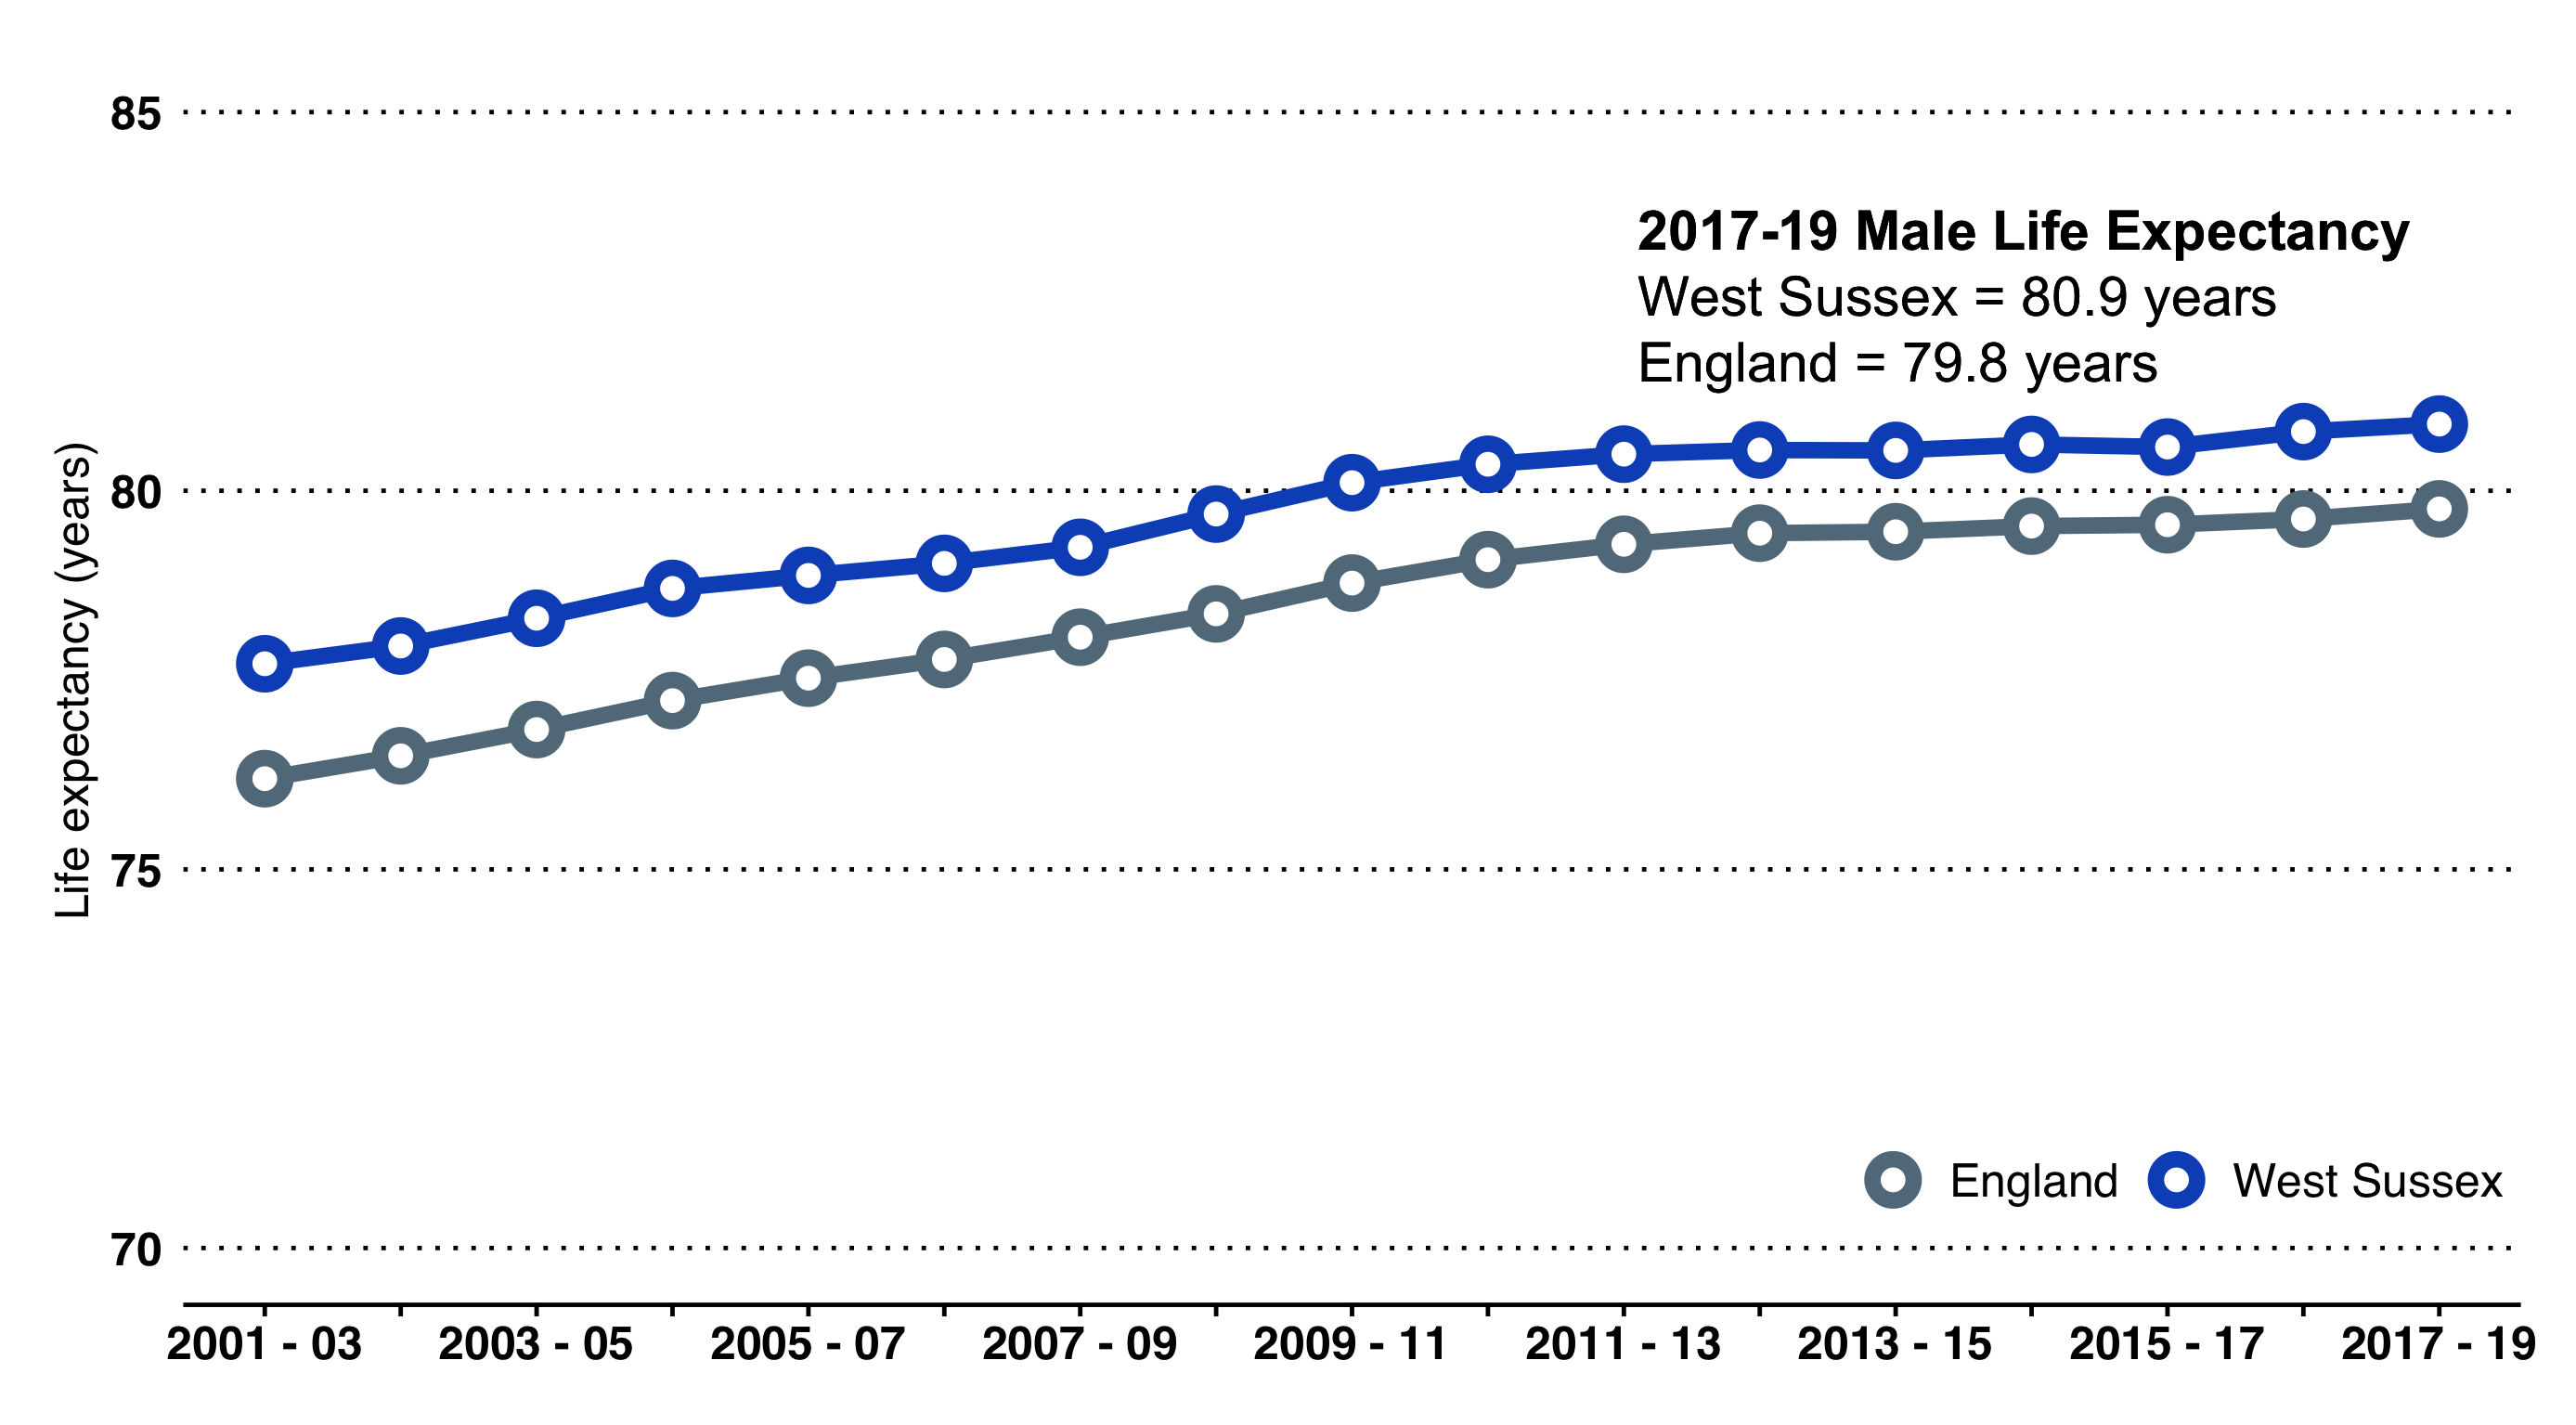
\includegraphics[width=\linewidth]{images/male_life_expectancy.png}
	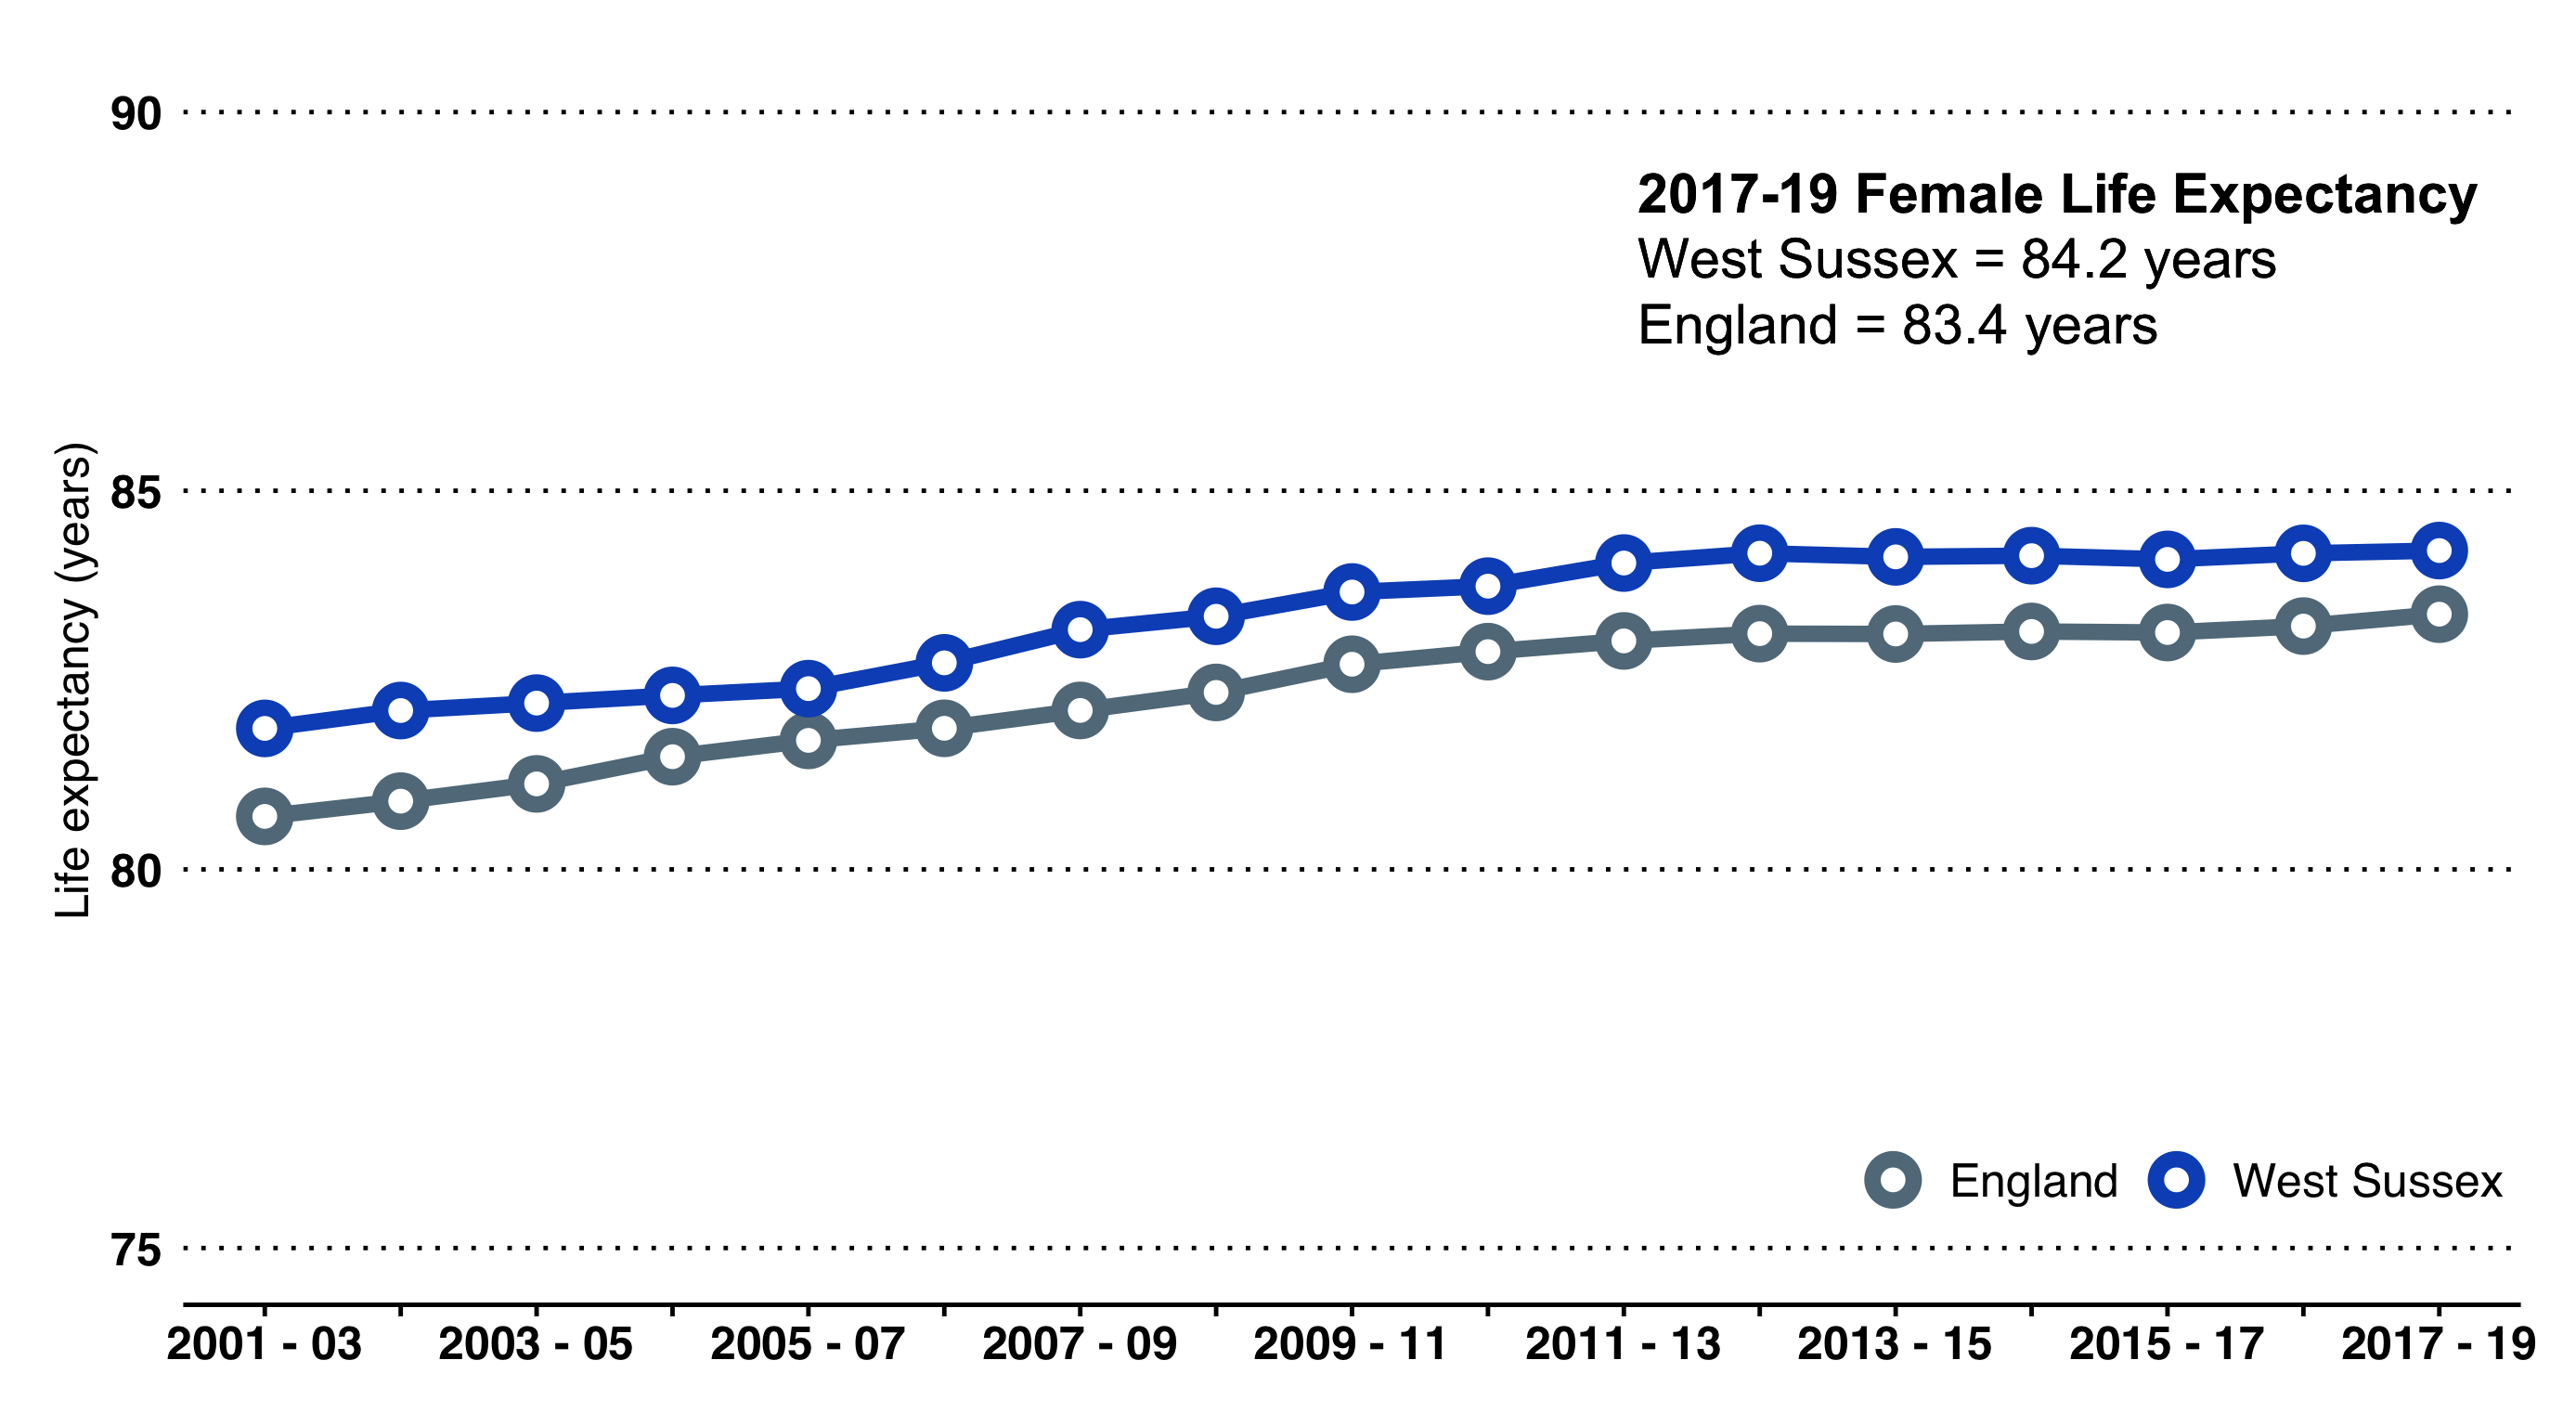
\includegraphics[width=\linewidth]{images/female_life_expectancy.png}
	\label{fig:life_exp}
\end{figure}

Difference in years of life expectancy between the least deprived and most deprived areas in West Sussex (2017-2019): Males from the most deprived area live on average 7 years fewer than males from the least deprived areas. Females from the most deprived areas live on average 6 years fewer than females from the least deprived areas.

For both men and women, circulatory causes (including stroke and heart disease) account for approximately a quarter of the difference, with cancers a further fifth of the difference\footnote{Note from OHID: Circulatory causes include heart disease and stroke}.

\begin{figure}[htp]
    \caption{Life expectancy gap between the most deprived quintile and least deprived quintile of West Sussex, by broad cause of death, 2015-17}
    \centering
	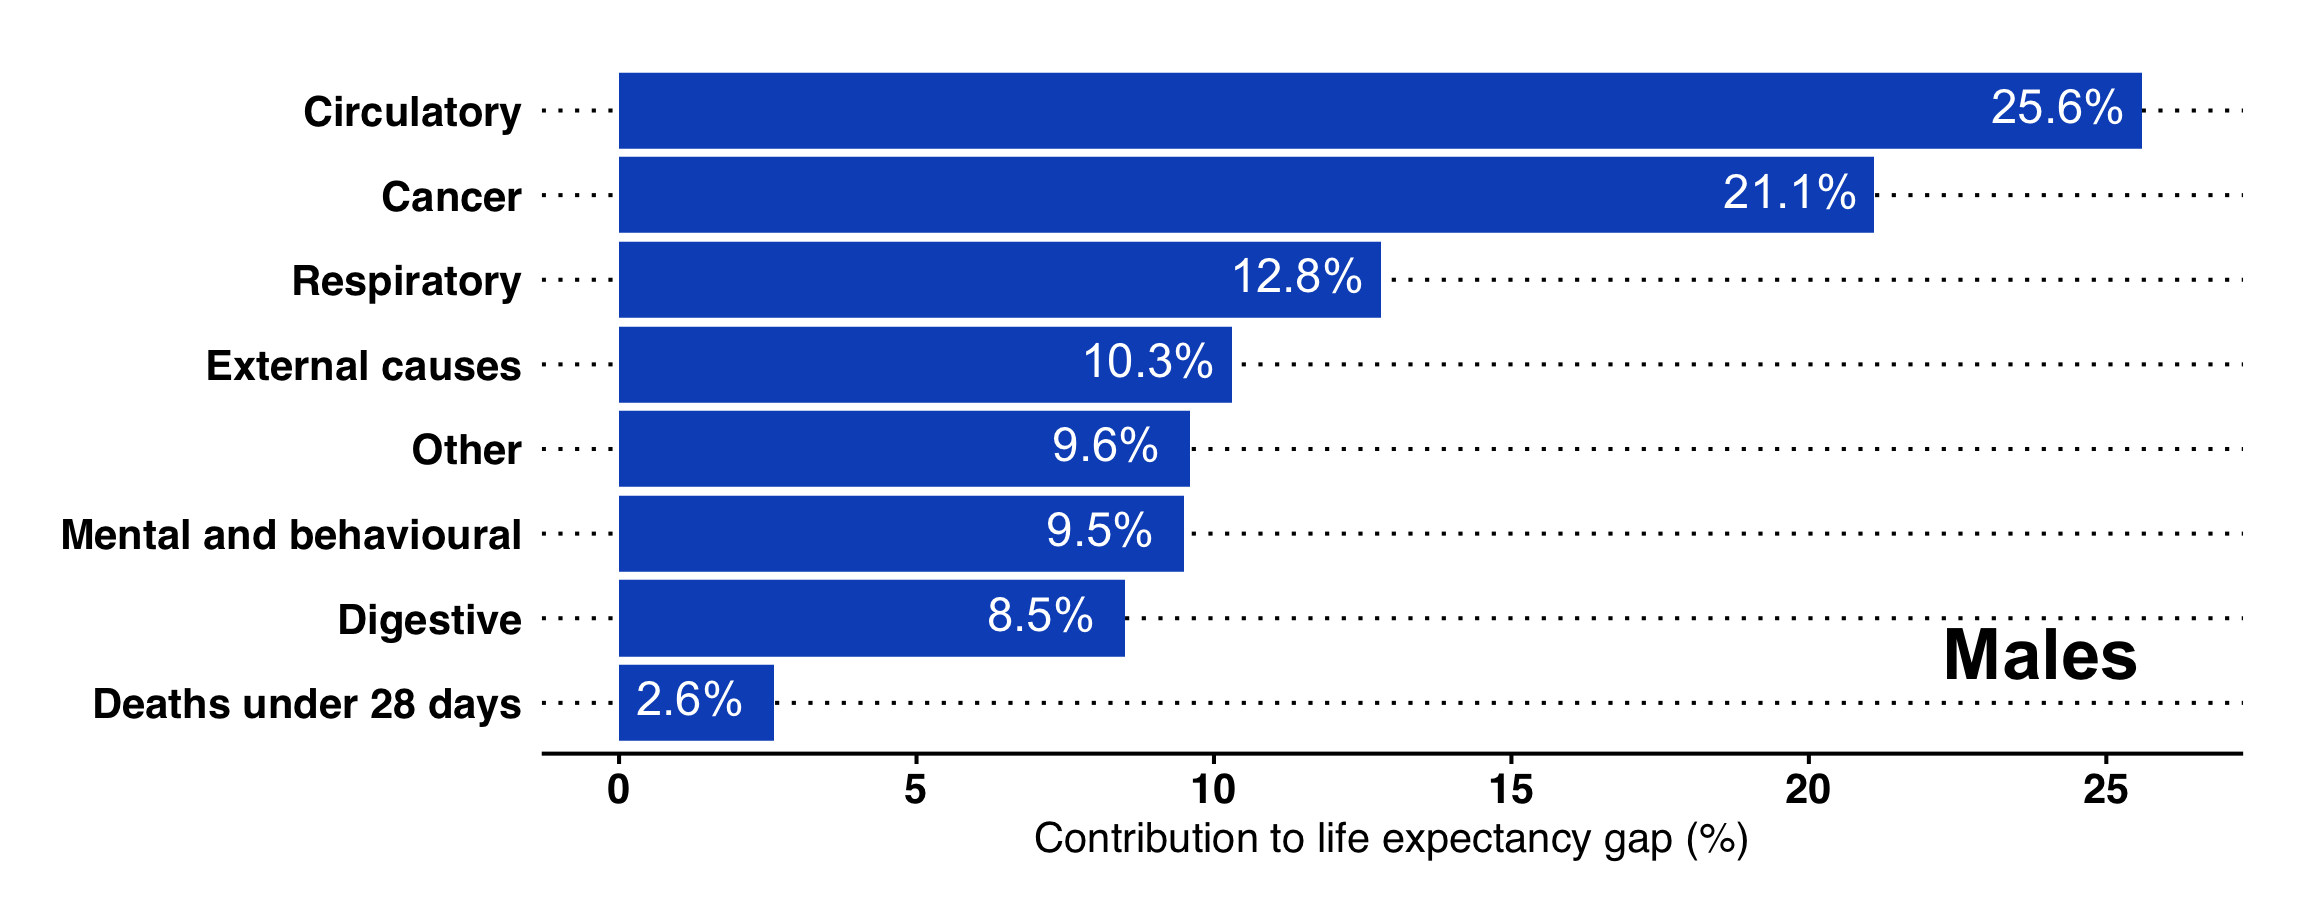
\includegraphics[width=\linewidth]{images/male_life_expectancy_gap.png}
	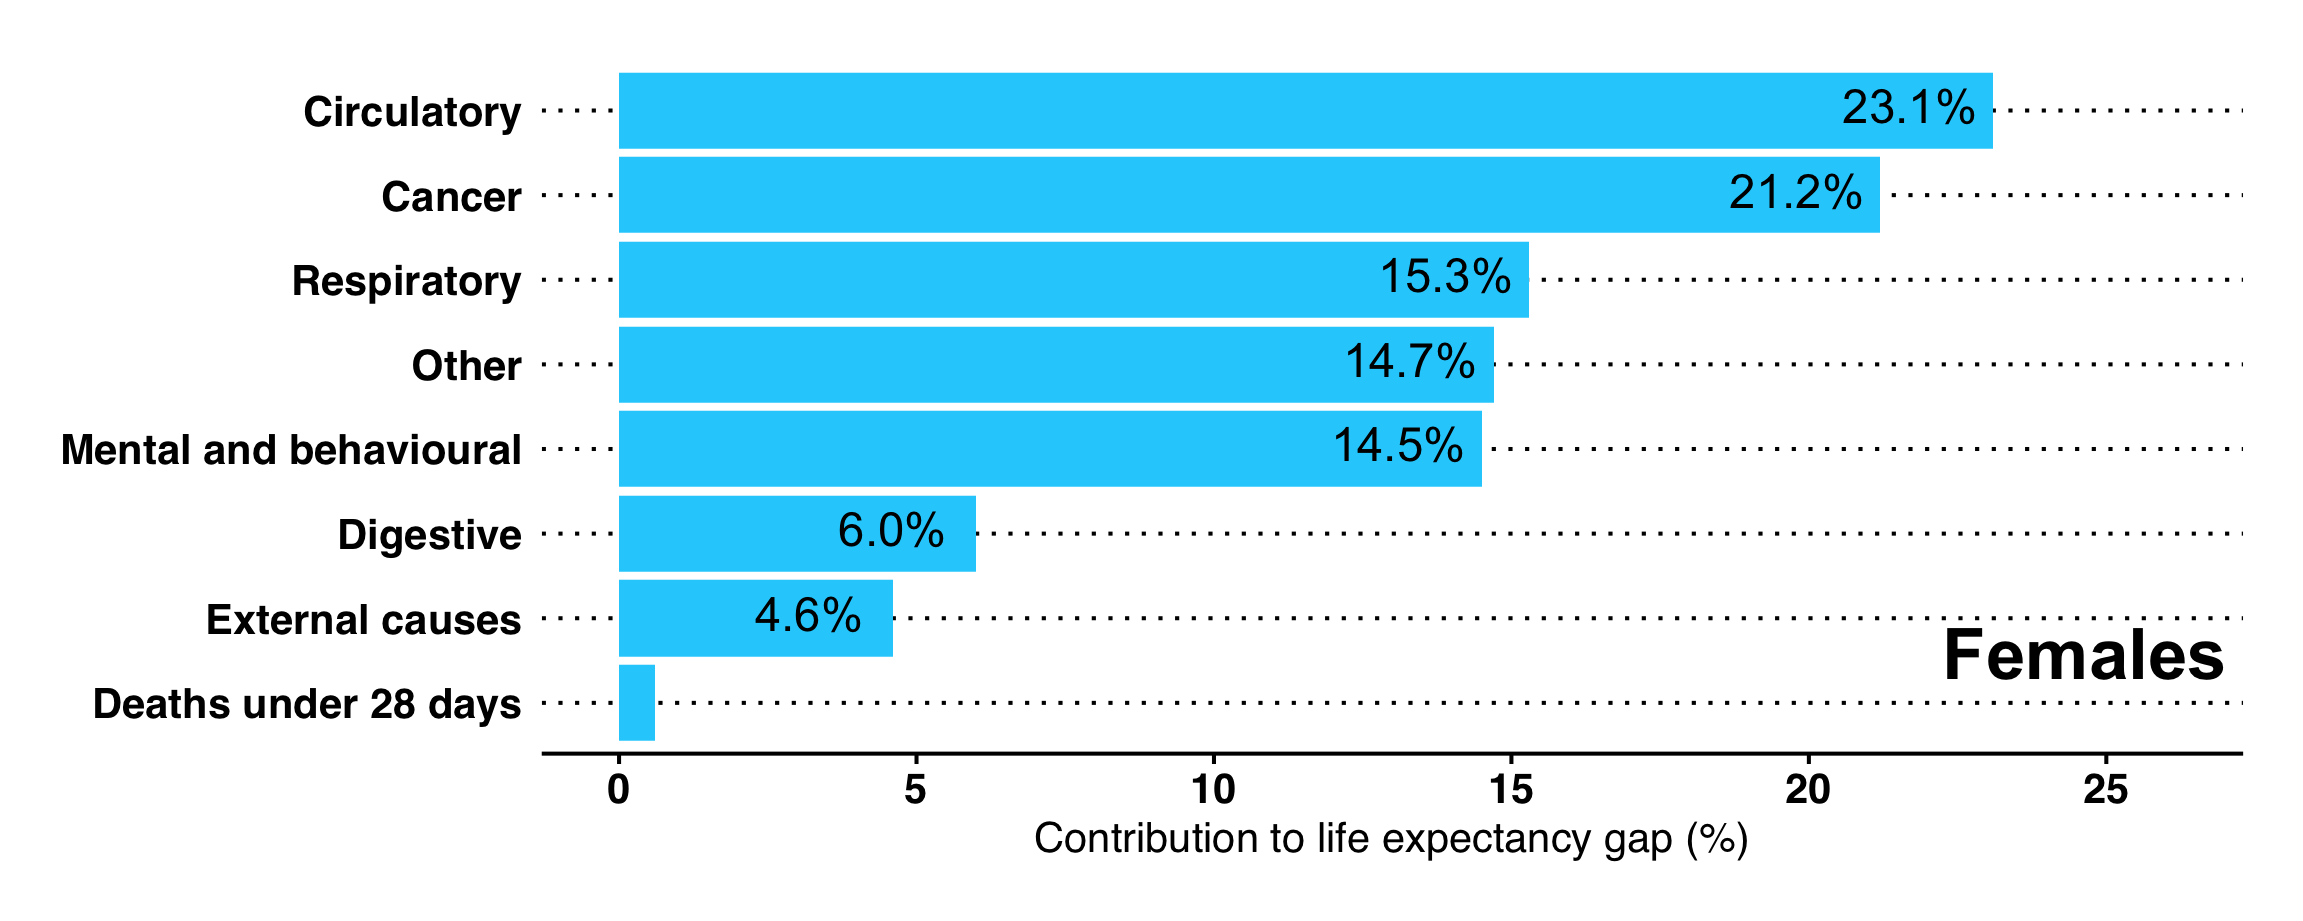
\includegraphics[width=\linewidth]{images/female_life_expectancy_gap.png}
	\label{fig:life_exp_gap}
\end{figure}

Respiratory includes flu, pneumonia, and chronic obstructive respiratory disease. Digestive includes alcohol-related conditions such as chronic liver disease and cirrhosis. External includes deaths from injury, poisoning and suicide. Mental and behavioural includes dementia and Alzheimer's disease. Percentages may not sum to 100 due to rounding.

PHE publish a segmentation tool to examine differences in life expectancy. Data are available at lower tier LA level \url{https://connect.healthdatainsight.org.uk/health_inequalities/segment_tool/}.

% \subsection{A focus on Social Mobility}
% \todo[inline]{This hasn't changed since last JSNA Summary (I think) so probably not worth repeating it, at least not in full.}
% The issue of social mobility has increased in prominence in recent years. In 2016, the Social Mobility Commission published data and ranked local authorities in terms of social mobility. The commission used a life stage approach looking at measures in the early years, school days, youth and adulthood. All 324 lower tier and unitary authorities were ranked, with the top 20\% performing areas, where social mobility opportunities were judged to be good, referred to as "hot spots" and the bottom 20\% of authorities, where opportunities are judged to be poor, as "cold spots". A summary is shown over the next two pages; the full briefing is available on the JSNA website. Contact Dr Verity Pinkney (\url{verity.pinkney@westsussex.gov.uk}) for further information.

% \paragraph{Key Points} Social mobility is about ensuring that young people have the same opportunities to succeed in life regardless of who they are or where they live. The social mobility index published by the Government\footnote{Note: This index was published in 2017 and some indicators will have changed since. The full report further explains the indicators behind the index. \url{https://www.gov.uk/government/publications/state-of-the-nation-2017}} looked at 16 key performance indicators which span our early years through to our working lives. This overall aim of the report was to answer the question: "What are the differences between local areas in the chances that a child from a disadvantaged socioeconomic background has of doing well as an adult?" There is a stark divide between London and the rest of the country, with nearly two-thirds of social mobility hotspots found in the capital. Arun, Chichester and Crawley were identified as social mobility cold spots on the overall index. Crawley was among the bottom 10\% of areas in England. Mid Sussex was the highest performer in West Sussex and was ranked 75th of the 324 local authorities in England.

% \paragraph{Younger people} Whilst the South East was the top performing region for early years, none of the local authorities in West Sussex were hotspots for this early age group and Chichester was a cold spot. Four local authorities in West Sussex were cold spots on the school age index. Crawley was the seventh worst in the country for school age. Of English local authorities, Crawley had the lowest proportion of children eligible for Free School Meals attending primary schools rated "good" or "outstanding" by OFSTED. Crawley was also identified as a cold spot for the youth index. Adults Horsham and Mid Sussex were hotspots on the adulthood index; this was due to high home ownership and fewer unskilled, low-paid jobs. Arun was the only local authority in West Sussex that was identified as a cold spot for adulthood.

% \paragraph{Crawley in Geographical Context - comparing Crawley with authorities bordering the M25} Crawley has a lot of assets, high employment and is close to London, yet it ranks low in terms of social mobility and now has areas ranked within the most deprived in the country. To understand Crawley in a wider geographic context, instead of comparing Crawley with the other West Sussex areas, we have looked at Crawley in context with 25 local authorities just outside the M25 (as a proxy for commuter belt areas), and deprivation relation to education and skills.

% This boxplot shows the ranks of small areas (LSOAs) within Crawley and 25 local authorities close to the M25, relating to education (KS2, KS4 and progression to higher education). A low rank means deprived, high rank means less deprived. In terms of education, Crawley is more deprived than the other authorities, with few areas within the town ranking in the less deprived deciles of the index of deprivation.

% FIGURE: Boxplot with ranks of small areas (LSOAs) within Crawley and 25 local authorities close to the M25, relating to education (KS2, KS4 and progression to higher education).

% \todo[inline]{Had a section here on the ICS - not sure now though}

%\subsection{An update on the ICS}

%How the primary care networks and clinical commissioning groups now slot in to the ICS picture.

%Website needs new single CCG profiles to replace the three former footprints.

%Do we want to have a subsection on pharmacies, perhaps in reference to Covid and vaccination?

%------------------------------------------------ % Intro
\newpage
\section{Starting Well}
% Need to go through with Verity and discuss the hot button issues that can be covered in this section
\subsection{Summary}
{\bfseries The early years of life lay foundations for lifelong physical, emotional and mental health, wellbeing and resilience. In tackling inequalities, action taken in the early years of life can have lifelong benefit, with many interventions being highly cost-effective.

There are 193,200 children and young people aged 0-19 years in West Sussex, with approximately 8,000 births a year. Across the county overall, 22\% of the population are 0-19 years, which is lower compared with England (24\%). Within the county, Crawley has a much younger population, with 26\% of residents aged 0-19 years.}

Overall measures of infant and maternal health in West Sussex are good, but inequalities are apparent across the county and in relation to specific groups. 
\begin{itemize}
    \item The infant mortality rate remains below the national rate (3.6 per 1,000 live births compared with 3.9 nationally)\footnote{PHOF E01, 2018-2020.}, we have fewer low birth weight babies, a lower percentage of women who smoke at the time of delivery, and a higher proportion of children who are assessed as having a good level of development at their two year check. 
\end{itemize}

However there remain challenges in the early years of life. 

\begin{itemize}[noitemsep]
    \item Many immunisation rates, whilst higher than national levels, remain below target levels.
    \item Measures relating to child readiness for school have improved in recent years but remain lower than many comparable authorities and for children eligible for a free school meal. For example, in 2018/19, approximately 72\% of children achieved a good level of development at the end of Reception whilst only 51\% were assessed as having a good level of development, the third lowest of comparable authorities.
\end{itemize}

We continue to observe a strong social gradient across many indicators and outcomes. Children living in poverty and from deprived areas are more likely to be overweight or obese; less likely to attain the expected level of attainment across educational key stages; more likely to admitted to hospital for self-harm; more likely to become pregnant as a teenager; and more likely to grow up in a household where someone smokes. 

In West Sussex, almost 17,000 children live in poverty. Children in poverty are more likely to come from single parent/carer families, be disabled or live in a household with an adult who is disabled. Poverty can transmit across generations and there are specific concerns about low social mobility in some parts of the county. 

It is also important to recognise that, on average, children who are in care or are care leavers have significantly poorer health and educational outcomes than their peers. 

Emotional and mental health are instrinically linked to physical wellbeing and longer term outcomes. Children who are happier and more emotionally resilient tend to have better physical health. Local survey data has highlighted the importance of cognitive reappriasal (reframing problems in a positive way) and expressive suppression (burying negative feelings/avoidance) in predicting life satisfaction and overall happiness\footnote{For more details, please see the 2019/20 JSNA Strategy.}.

% Children in low income families can be found on Stat-x-plore https://stat-xplore.dwp.gov.uk/webapi/jsf/dataCatalogueExplorer.xhtml

% \subsection{Impact of Covid-19 Pandemic}
% \todo[inline]{Use the WICH tool to support this part of the narrative. Some of the indicators involve children and young people. November 2021 access.}

\subsection{Infant and Maternal Health}
Key demographic information and health indicators are summarised in the West Sussex Local Health Profiles for Children and Young People 2020, available on the JSNA website.

\subsubsection{Infant and Maternal Health}
{\bfseries In 2020 there were 8,001 births,} the lowest number in West Sussex since 2006. The infant mortality rate\footnote{PHOF reference E01, defined as the number of deaths in infants aged under 1 year per 1,000 live births.} in 2018-2020 was 3.6 per 1,000 live births, lower than the national rate of 3.9 per 1,000, although a slight increase on the previous three years.

The {\bfseries neonatal mortality rate} (defined as the number of deaths under 28 days, per 1,000 live births) has remained stable over the past 10 years, although there has been a slight rise in both 2017-2019 and 2018-2020. The rate in West Sussex 3.6 per 1,000 live births, in line with the England rate (3.9 per 1,000) and below the median of the south east region. 

{\bfseries The percentage of term babies with low birth weight (less than 2500g; \footnote{PHOF reference C04.}) remains steady}, at 2.04\% in 2020, and significantly lower than England (2.9\%) and in the lowest three of CIPFA neighbours.

In 2018-20, there were {\bfseries 78.6 premature births (less than 37 weeks gestation) per 1,000} live births and still births, which is the lowest it has been since 2011-13 (76.6 per 1,000). The rate in West Sussex has followed national trends, and is in line with the England rate of 79.1 per 1,000.

The multiple birth rate (the number of maternities with multiple births per 1,000 total maternities) in 2020 was 11.0 ({\bfseries 87 multiple births}), lower than the England rate of 14.4.

{\bfseries In 2020/21, 34.1\% of births were by caesarean section in West Sussex.} This proportion has been increasing over the last 5 years and is significantly higher compared to England (32.5\%) and is also the second highest among five comparable authorities\footnote{NOTE: these comparable authorities are not the standard CIPFA neighbours, but rather the Children's Services Statistical Neighbours as provided by LAIT.}.

{\bfseries The percentage of women smoking at the time of delivery\footnote{PHOF reference C06. Note: the method used to calculate this outcome was changed in April 2017, excluding women with unknown smoking status from the denominator when calculating the proportion of women smoking at the time of delivery.} remained low in 2020/21 at 8.5\% (approximately 678 maternities)}, lower than the national rate and the second lowest of comparable authorities.

In 2019/20, 55.7\% of women breastfed (wholly or partly) at 6-8 weeks\footnote{PHOF reference C05b.}. Nationally, the figure was 48\%. West Sussex was the second highest of comparable authorities. Note that this indicator is not available for 2020/21 due to data quality issues.

In 2020/21, 91.5\% of New Birth Visits (NBVs)\footnote{PHOF reference C07. All infants and their families are eligible to receive a visit led by a health visitor within the first two weeks from birth, as part of the Healthy Child Programme and to ensure continuing support following midwife visits, which usually end at day 10. For 2020/21, this indicator was scaled up from three quarters worth of available data.} were completed within 14 days this has increased to be above the England rate (88.0\%).

In 2020/21, 84\% of children assessed achieved a good level of development at 2-2½ years\footnote{PHOF reference C08a. For 2020/21, this indicator was scaled up from three quarters worth of available data.}, comparing well with England (82.9\%), and making West Sussex the fifth highest amongst comparable local authorities.

Uptake of the flu vaccine in 2-3 year-olds\footnote{PHOF reference D03l.} in 2020/21 was 67.5\% and was significantly higher than England (56.7\%) and the $\geq$65\% benchmark.

% \todo[inline]{check MEASLES}In 2018, there were 45 laboratory confirmed cases of measles in West Sussex, representing a rate of 5.3 per 100,000 population, the highest amongst comparable authorities and the 16th highest in England.

\subsubsection{Maternal Mental Health} In relation to maternal mental health, it is estimated that between 10\% and 20\% of women will be affected by mental health problems, either during their pregnancy or in the first year post delivery. Local data are scarce but using synthetic estimates provided by Public Health England, the number of mothers with specific problems are shown below (note some women will be affected by one or more problems):
\begin{itemize}[noitemsep]
    \item Postpartum psychosis: 20 
    \item Chronic Severe Mental Illness: 20
    \item Severe depressive illness: 250 
    \item Mild-moderate depressive illness and anxiety: 830 (lower estimate) to 1,245 (upper estimate) 
    \item PTSD: 250 
    \item Adjustment disorders and distress: 1,245 (lower estimate) to 2,485 (upper estimate)
\end{itemize}

\subsection{West Sussex Childhood Vaccine and Immunisation Coverage Rates}
See Table~\ref{tab:childhoodimms} on page~\pageref{tab:childhoodimms}.
\begin{table*}[hbt]
    \scriptsize
    \caption{West Sussex Childhood Vaccine and Immunisation Coverage Rates. PHOF references (all, except Hib/Men C booster in under-5s are PHOF indicators) D03b to D03f; D03h to D03m; D04a to D04c; D04e; D04f; Cl.2}
    \centering
    \begin{tabular}{llrrrr}
    \toprule
    Immunisation &  Detail & Year & \% Coverage & Lower CI & Upper CI \\
    \midrule
    Rotavirus & \% of children who have received the rotavirus vaccine by 6 months of age & 2019/20	& 91.90\% & 91.40\% & 92.50\% \\
    Hepatitis B & \% of children at age 12 months who have received the complete course (3 doses) of hepatitis B vaccine. & 2019/20	& 100\% & 75.80\% & 100\% \\
    DTaP / IPV / Hib & \% of children who received 3 doses of DTaP/IPV/Hib vaccine at any time by their rst birthday. & 2019/20	& 95.40\% & 94.40\% & 96.50\% \\
    MenB & \% of children who received the MenB vaccine at any time before their rst birthday & 2019/20	& 95.40\% & 94.90\% & 95.80\% \\
    PCV & \% of children who received two doses of PCV at any time before their first birthday. & 2019/20 & 95.80\% & 95.30\% & 96.20\% \\
    MenC & \% of children who received 2 doses of MenC vaccine at any time by their rst birthday. & 2015/16 & 94.3 & 93.8 & 94.7 \\
    Hib / MenC booster & \% of children who received a booster dose of Hib/MenC at any time before 2nd birthday. & 2019/20 & 94.60\% & 94.20\% & 95.10\% \\
    MMR one dose & \% of children who received one dose of MMR on or after their first birthday and at any time before their 2nd birthday. & 2019/20 & 94.70\% & 94.30\% & 95.20\% \\
    Hepatitis B & \% of children at age 24 months who have received the complete course (4 doses) of hepatitis B vaccine. & 2019/20 & suppressed & - & - \\
    DTaP / IPV / Hib & \% of children who received 3 doses of DTaP/IPV/Hib at any time before their 2nd birthday & 2018/19 & 95.7 & 95.3 & 96.1 \\
    PCV booster & \% of children who received a booster dose of PCV at any time before their 2nd birthday & 2019/20 & 94.40\% & 93.90\% & 94.90\% \\
    MenB booster & \% of children who received a booster dose of MenB at any time before their 2nd birthday & 2019/20 & 93.20\% & 92.70\% & 93.70\% \\
    Flu & \% children aged 2-3 years old, who received the Flu vaccination (1st Sept to the end of Feb) in a primary care setting & 2019/20 & 53.50\% & 52.80\% & 54.30\% \\
    DTaP / IPV & \% of children who received a booster dose of DTaP/IPV at any time before their fifth birthday & 2019/20 & 89.30\% & 88.60\% & 89.90\% \\
    MMR for one dose & \% of children who received one dose of MMR on or after their first birthday and at any time before their fifth birthday. & 2019/20 & 95.70\% & 95.20\% & 96.00\% \\
    MMR for two doses & \% of children who received two doses of MMR on or after their first birthday and at any time before their fifth birthday. &  2019/20 & 91.60\% & 91.10\% & 92.10\% \\
    Hib / Men C booster & \% of children who received a booster dose of Hib/MenC at any time before their fifth birthday. & 2017/18 & 92.6 & 92.1 & 93.1 \\
    HPV - one dose & \% of females in school year 8 (aged 12-13) who have received the first dose of HPV vaccine & 2019/20 & 14.90\% & 13.90\% & 15.90\% \\
    HPV - two doses & \% of females in school year 8/9 (aged 13-14) who have received the second (completing) dose of HPV vaccine & 2019/20 & 11.30\% &10.40\% & 12.30\% \\
    \bottomrule
\end{tabular}
\label{tab:childhoodimms}
\end{table*}
\normalsize
\subsection{Hospital admissions}
\paragraph{Emergency admissions}In 2020/21, West Sussex had among the highest emergency hospital admission rates in the South East, and rates were higher than national rates:
\begin{itemize}[noitemsep]
    \item {\bfseries Under 1 years old -- 2,500 admissions,} a rate of 253.4 per 1,000 population.
    \item {\bfseries 0-4 year olds -- 4,880 admissions,} a rate of 107.4 per 1,000 population.
    \item {\bfseries Under 18s -- 9,480 admissions,} a rate of 53.4 per 1,000 population.
\end{itemize}
\paragraph{Admissions to hospital - 0-19 year olds}
\begin{itemize}[noitemsep]
    \item {\bfseries Asthma -- 100 admissions (2020/21)}, a rate of 53.8 per 100,000 population, lower than England and comparable authorities.
    \item {\bfseries Diabetes -- 115 admissions (2019/20)}, a rate of 62.2 per 100,000 higher than England and comparable authorities.
    \item {\bfseries Epilepsy -- 125 admissions (2019/20)}, a rate of 67.6 per 100,000, similar to England and comparable authorities.
\end{itemize}

\subsection{Disability through the life course}
\paragraph{Overall Disability Assumption} The term "disability" is frequently used but often poorly defined, and estimating the prevalence and type of disability within a population is difficult. The purpose of a definition (for example, for deciding educational support vs. eligibility for welfare benefits), as opposed to a "formal diagnosis" can mean that different sources can often provide very different pictures of the local population.

The Family Resources Survey (FRS) is a national, continuous household survey that collects data on a wide range of information including disability\footnote{{\bf The definition of "disability" in the Family Resource Survey is} used to describe people who identify themselves or have been identified as having any physical or mental health condition or illness that lasts or is expected to last 12 months or more, and acts to limit the ability to carry out day-to-day activities. While this will capture most people under the definition used in the Equality Act 2010, it should be noted that there will be some people under the 2010 Act who are classified as disabled (and having rights under the Act) who have a long-standing illness or disability which is not currently affecting their day-to-day activities e.g. some people who have a diagnosis of cancer will not be included.}, caring, tenure and income. One of the main functions of the survey is to inform the Department of Work and Pensions (DWP) of the living conditions and economic circumstances of different households. Small sample size means that data are not published below regional level. Using the results from the latest national survey and applying the prevalence to the local population provides a local estimate of disability by age groups. Given that West Sussex overall has a relatively healthy and wealthy population, these estimates may be higher than expected and should be treated as possibly high estimates.

\begin{figure}[htp]
    \caption{Disability by age group and gender}
    \centering
	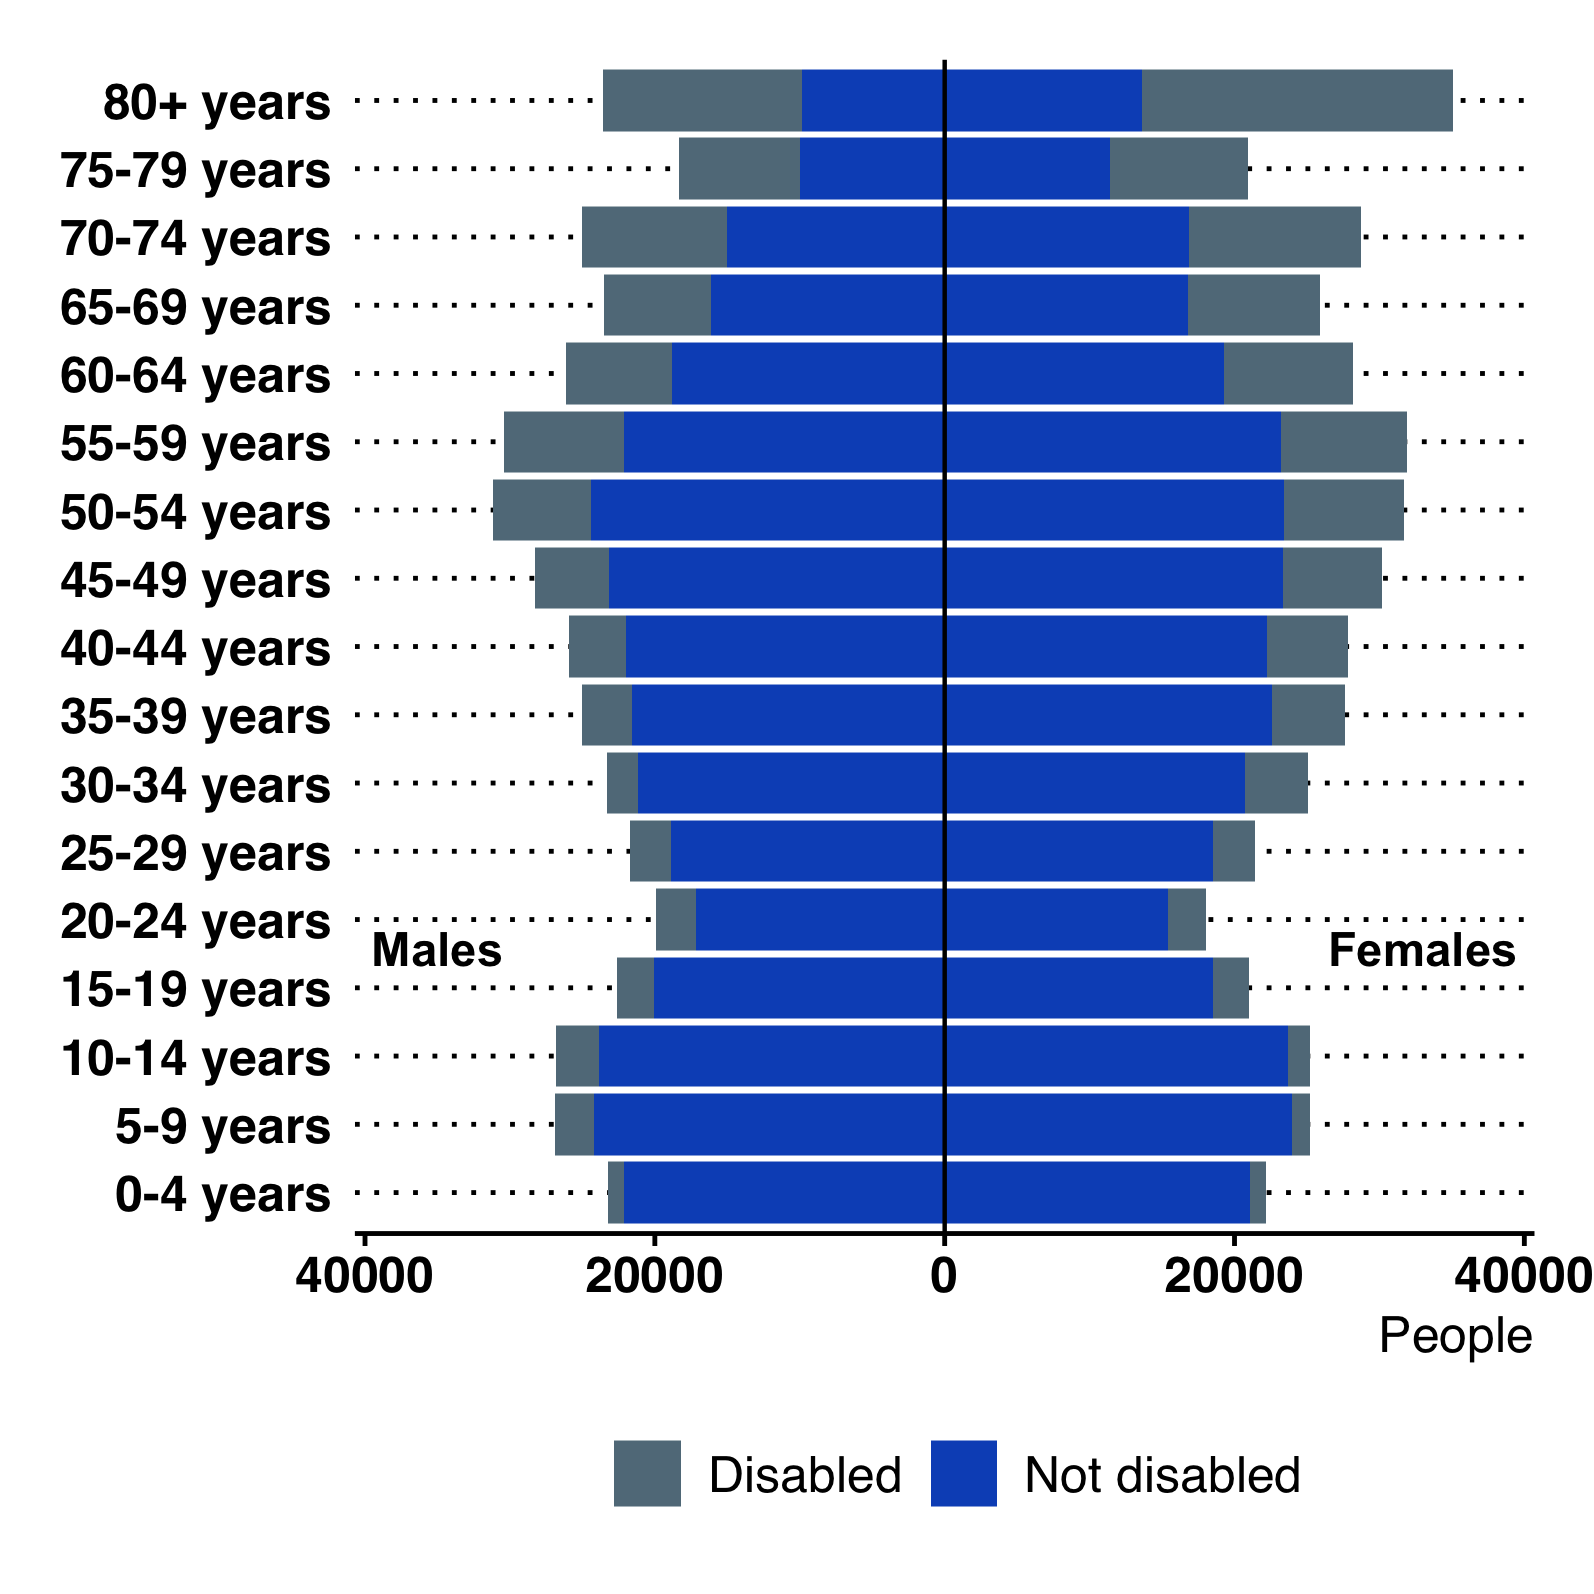
\includegraphics[width=\linewidth]{images/frs_disability_wsx.png}
	\label{fig:frs_diab_wsx}
\end{figure}

FRS Disability Prevalence (average of years 2014/15 to 2017/18) Applied to 2018 West Sussex Population TABLE\todo[inline]{Where did I put this?}

\paragraph{FRS Type of Impairment} Of people who described themselves as being disabled, data were also collected on the nature of their impairment. As people are able to state multiple impairments, figures in Table~\ref{tab:impairment} do not sum 100.

Nationally it is noted that the proportion of FRS respondents who reported a mental health impairment has been rising in recent years, from 22\% in 2015/16 to 25\% in 2017/18.\todo[inline]{Check this}

Note again that, given West Sussex overall has a relatively healthy and wealthy population, these estimates may be higher than expected and should be treated as possibly high estimates.

\begin{table}[hbt]
    \caption{FRS Type of Impairment}
    \centering
    \begin{tabular}{lllll}
    \toprule
    Impairment & All Disabled & Children & Working & State \\
    type (\%) & People & \ & age & Pension \\
    \midrule
    Mobility & 49 & 19 & 41 & 67 \\
    Stamina, breathing \& fatigue & 37 & 24 & 32 & 46 \\
    %and fatigue & \ & \ & \ & \ \\
    Dexterity & 26 & 11 & 23 & 34 \\
    Mental health & 25 & 23 & 38 & 9 \\
    Memory & 16 & 11 & 16 & 17 \\
    Hearing & 14 & 8 & 8 & 23 \\
    Vision & 12 & 9 & 9 & 18 \\
    Learning & 13 & 36 & 14 & 8 \\
    Social/behavioural & 9 & 43 & 10 & 2 \\
    Other & 17 & 18 & 18 & 15 \\
    \bottomrule
    \end{tabular}
    \label{tab:impairment}
\end{table}

\subsection{Mental Health and Wellbeing}
{\bfseries Major national surveys remain the best source of evidence on the prevalence of mental health disorders among children and young people.}

In 2004, ONS conducted a national survey to estimate the prevalence of mental health conditions in children aged 5-16\footnote{NHS Digital: Mental health of children and young people in Great Britain (2004)}. Public Health England has applied the survey results to local populations taking into account age, sex and socio-economic classification\footnote{As part of the PHE CYP mental health and wellbeing profile (Fingertips)}. In 2015, 8.4\% of children and young people aged 5-16 were estimated to have a mental health condition in West Sussex. This equates to around 9,500 children. Since there is evidence to suggest that prevalence of mental health conditions among children and young people has increased, it is possible that this represents an underestimate.\todo[inline]{Update this?}

\begin{table}[hbt]
    \caption{Estimates from the 2004 Survey applied to 2015 Population}
    \centering
    \begin{tabular}{llr}
    \toprule
    Type of & Estimated 2015 & Number of CYP \\
    disorder & prevalence among CYP & \ \\
    \midrule
    Mental health & 8.4\% & 9,490 \\
    Emotional & 3.2\% & 3,655 \\
    Conduct & 5.0\% & 5,635 \\
    Hyperkinetic & 1.3\% & 1,515 \\
    \bottomrule
    \end{tabular}
    \label{tab:yp:mh1}
\end{table}

The 2004 survey has now been updated with a new series of data collection completed in 2017\footnote{NHS Digital: Mental Health of Children and Young People in England (2017)}. NHS Digital released the findings from this survey in 2019. This goes beyond the 2004 survey, providing estimates of the prevalence of mental health disorder in 2 to 4 year olds, and spans the transition into adulthood covered by 17 to 19 year olds.

The main findings from the 2017 survey include:
\begin{itemize}[noitemsep]
    \item {\bfseries One in eight (12.8\%) 5 to 19 year olds and one in eighteen (5.5\%) preschool children assessed had at least one mental health disorder}
    \item {\bfseries Rates of mental health disorders increased with age.} Young people aged 17 to 19 were three times more likely to have a mental health disorder (16.9\%) than preschool children aged 2 to 4 (5.5\%), although data collection methods varied by age
    \item {\bfseries Young women were identified as a high a risk group in relation to mental health,} with nearly one in four (23.9\%) 17 to 19 year old girls identified as having a mental disorder
    \item {\bfseries Prevalence of mental disorders also varied by ethnicity} (higher in White British children) and by socioeconomic status (higher among children living in lower income households)
    \item {\bfseries Emotional disorders were the most prevalent type of disorder experienced} by 5 to 19 year olds in 2017 (8.1\%)
    \item {\bfseries Behavioural disorders were the most prevalent (2.5\%) for preschool children}
    \item {\bfseries Trend analyses revealed a slight increase over time in the prevalence of mental disorder} in 5 to 15 year olds
    \item {\bfseries Emotional disorders have become more common in 5 to 15 year-olds,} whilst prevalence of other mental health disorders have remained similar over time
    \item {\bfseries Most children with a disorder who had used professional services tended to view them as helpful.} Primary care was the service most likely to be rated as unhelpful; 17.0\% of 5 to 19 a year olds with a disorder who had contact with a primary care a professional due to worries about mental health described the contact as unhelpful or very unhelpful.
\end{itemize}

\paragraph{Wave 2 follow up to the 2017 survey}
Published in September 2021, the wave 2 follow up to the 2017 survey\footnote{/url{https://digital.nhs.uk/data-and-information/publications/statistical/mental-health-of-children-and-young-people-in-england/2021-follow-up-to-the-2017-survey}} examined the mental health of 6 to 23 year olds living in England in 2021 and describes their experiences of family life, education, and services during the coronavirus (COVID- 19) pandemic. Comparisons were made between 2017 and 2020 (where possible), to monitor changes over time.

The key findings were:
\begin{itemize}
    \item Probable mental disorder: Rates of probable mental disorder increased between 2017 and 2021; in 6 to 16 year olds from one in nine (11.6\%) to one in six (17.4\%), and in 17 to 19 year olds from one in ten (10.1\%) to one in six (17.4\%). Rates in both age groups remained similar between 2020 and 2021.
    \item Change in mental health: Looking at individual-level change, 39.2\% of those aged 6 to 16 years in 2021 had experienced deterioration in mental health since 2017, and 21.8\% experienced improvement. Among those aged 17 to 23 years in 2021, 52.5\% experienced deterioration, and 15.\% experienced improvement.
    \item Eating problems: The proportion of children and young people with possible eating problems increased between 2017 and 2021, from 6.7\% to 13.0\% in 11 to 16 year olds and from 44.6\% to 58.2\% in 17 to 19 year olds.
    \item Sleep problems: In 2021, problems with sleep on three or more nights of the previous seven affected over a quarter (28.7\%) of 6 to 10 year olds, over a third (38.4\%) of 11 to 16 year olds, and over half (57.1\%) of 17 to 23 year olds. Across all age groups figures were much higher in those with a probable mental disorder (59.5\%, 74.2\%, 86.7\% respectively).
    \item School absence: Overall, 10.6\% of 6 to 16 year olds missed more than 15 days of school during the 2020 Autumn term. Children with a probable mental disorder were twice as likely to have missed this much school (18.2\%) as those unlikely to have a mental disorder (8.8\%).
    \item Learning resources: The proportion of 6 to 16 year olds with a laptop or tablet they could work on at home, increased from 89.0\% in 2020 to 94.4\% in 2021. The proportion receiving regular support from school or college also increased, from 73.7\% in 2020 to 79.9\% in 2021.
\end{itemize}

\paragraph{Estimated prevalence by CAMHS "Tier" in West Sussex} Mental health services are often described in terms of tiers, where services become more specialised, from emotional wellbeing services at Tier 1 to highly specialist outpatient teams and inpatient provision at Tier 4. Prevalence estimates (population aged 17 and under) based on findings published in "Treating Children Well"\footnote{Kurtz, Z. (1996) Treating children well: a guide to using the evidence base in commissioning and managing services for the mental health of children and young people. London. Mental Health Foundation.} are shown below against each of the tiers. These provide an estimate of West Sussex children and young people who may at any one time, need a service response or support.

FIGURE - Tier Pyramid\todo[inline]{quick version of this needed for diagrammatic purposes - can I set it next to the table using LaTeX?}

\begin{table}[hbt]
    \caption{Estimated prevalence by CAMHS tier}
    \centering
    \begin{tabular}{lrr}
    \toprule
    Tier - service & Prevalence & Estimated number \\
    provision & assumption & of children \\
    \midrule
    Tier 4 & 0.075\% & 130 \\
    Tier 3 & 1.85\% & 3,230 \\
    Tier 2 & 7.00\% & 12,225 \\
    Tier 1 & 15.00\% & 26,200 \\
    \bottomrule
    \end{tabular}
    \label{tab:yp:camhs-tiers}
\end{table}

 
\subsection{Autism}
There are a number of problems estimating the number of people who have autism:
\begin{itemize}
    \item There is no single source or register, and setting one up would be difficult to maintain.
    \item Not all people will have been diagnosed and some people may have been misdiagnosed.
    \item There are inconsistencies in how agencies record autism.
    \item Much of the existing work on prevalence has been undertaken in relation to children; there may be enduring problems of childhood misdiagnosis or some people only being diagnosed in adulthood.
    \item There is some evidence of poor identification of adults with autism compared with children.
\end{itemize}

{\bfseries In the 2019 school census, there were 1,317 school pupils with special educational needs who had primary need of autism spectrum conditions} in West Sussex. A major survey\footnote{NHS Digital: The Mental Health of Children and Young People in England, 2017 survey} of the mental health of children and young people identified autism spectrum conditions in 1.2\% of 5 to 19 year olds. Due to the small number of cases identified in this sample and the sampling method used (such as self-report only for 17-19 year olds), it is possible that this reflects an underestimate. {\bfseries Applying this prevalence estimate to the local population of 5 to 19 year olds in West Sussex suggests that there are around 1,700 autistic children and young people in the county.}

\paragraph{Statement from the West Sussex Autism Partnership Board} In collating and publishing data for the JSNA summary it is important to acknowledge that for some health issues and conditions there is a lack of robust local and/or national data; this can have implications in terms of accessing services and receiving appropriate support. A statement from the West Sussex Autism Partnership Board is included below:

{\itshape 'The Autism Partnership Board acknowledges that there is a lack of accurate data about the actual numbers of autistic adults and our concern is that if there is under- reporting this will result in not enough support services being commissioned to meet need. The Board felt that the method of researching prevalence exacerbates the issue of underreporting and potentially discriminates against autistic individuals and others with communication differences.

Autistic adults face many challenges. Often, they also have co-occurring conditions such as a learning disability or mental health problems. For some they feel they have a 'hidden' condition which is not easily recognised or understood by professionals or the public. Locally, two of the key issues for autistic adults are the 20 month waiting time for a diagnosis and the risk of falling into the gap between learning disability and mental health services so that people could struggle to get the help they need. The Neurodevelopmental services report that receiving a diagnosis can be transformation for many individuals who experience mental health problems as a result of their needs in relation to autism not being understood. A diagnosis can have a preventative function in this regard in addition to leading to reasonable adjustments that improve mental health outcomes.

Commissioners require a more robust understanding of the numbers of autistic people - for example those registered with a GP - and an understanding of how well people's needs, of all ages, are being met and what outcomes are being achieved, for example in employment and housing, and in Public Health data on higher mortality rates and poorer physical health outcomes'.}

%\subsection{A Focus on Self-harm}
%{\bf Note}: On the next few pages we focus on the {\bfseries prevalence of self-harm and hospital admissions}. This is a relatively limited view of the problem, and self-harm that results in a hospital admission may be different in nature than self-harm that doesn't. We have used this measure as there is a lack of robust local data outside of hospital statistics. {\bfseries\itshape Self-harm affects all ages; as behaviour in childhood can often persists into adulthood, information on self-harm in all age groups has been placed in the Starting Well section.}

%A rapid needs analysis was undertaken in 2019, which provides more detail and context including how self-harm is defined*, the extent of self-harm in West Sussex, who is most at risk, what can be done, and what is being done locally. This report is on the JSNA website. 

%For further information contact Rachel Jevons (Public Health lead for mental health) \url{rachel.jevons@westsussex.gov.uk} or Verity Pinkney (who provided the analysis) \url{verity.pinkney@westsussex.gov.uk}


%\paragraph{Overall} {\bf In 2018/19 there were 1,845 emergency admissions for self-harm in West Sussex\footnote{PHOF reference C14b. This is also an outcome on the West Sussex Plan.}}; as a rate per 100,000 this is significantly higher than the England average. Looking over a six year period from 2013/14 to 2018/19, there were 11,099 emergency hospital admissions for self-harm in West Sussex, with an age standardised rate of 235.9 per 100,000 persons.

%Figures suggest that every admission for self-harm through self-poisoning costs £806, with self-injury costing £753. Based on these costs, the current burden for West Sussex is in the order of £1.3m to £1.4m. When the broader costs to society (economic, educational, unpaid care etc) are taken into account this rises to £6.2m - £6.6m per annum.

%\paragraph{Inequalities} Across West Sussex, rates of self-harm vary; Adur, Arun and Worthing have exceeded the national rate since 2010/11, whilst Horsham and Mid Sussex tend to be more comparable to the England average (although Mid Sussex has seen a significant rise from 2016/17 to 2018/19). There are marked inequalities in self- harm, with higher rates among areas with greater deprivation.

%In 2017/18, young people aged 15-19 accounted for a fifth of all emergency hospital admissions for self-harm in West Sussex, at around 350 admissions. The proportion of emergency admissions for self-harm is highest among young people and generally decreases with age thereafter. In total, young people aged 10-24 account for 39\% of all admissions for self-harm in West Sussex.

%Some people had multiple admissions; around 50 individuals (2\% of total number of people) accounted for 370 self-harm admissions that occurred in 2016/17 to 2017/18 (11\% of total number of admissions). These persons were admitted for self-harm 5 or more times during the 2 year period.

%\paragraph{Forms of Self-Harm} In the five years from 2013/14 to 2017/18, 88\% of admissions were due to self- poisoning and the majority of those were from widely available over the counter medicines, such as paracetamol. Self-harm through use of sharp objects accounted for some 9\% of all admissions for this period.

%While {\bf self-poisoning was associated the majority of admissions in West Sussex, national data suggests that self-cutting is the most common form of self-harm overall.}

%\paragraph{Self-harm definition} {\bf As outlined in the West Sussex Rapid Needs Analysis:} There are a number of definitions of self-harm.......We will follow the example from our neighbours in Brighton \& Hove Council and Brighton \& Hove Clinical Commissioning Group (CCG) and take a pragmatic approach, using the more inclusive definition provided by the National Self-Harm Network: {\bf "Self-harm can take many different forms and as an individual act is hard to define.} However, in general, self-harm (also known as self-injury or self-mutilation) is {\bf the act of deliberately causing harm to oneself either by a causing a physical injury, by putting oneself in dangerous situations, and/or self-neglect.}

%\paragraph{Self-harm in tables and charts.... }

%FIGURE: Proportion of emergency admissions for self-harm by age and sex (2017/18) 

%Data continues to show that differences by sex are most pronounced at younger ages. Among 10-24 year olds, 80\% of emergency admissions for self-harm in West Sussex were females (2017/18).

%\begin{table}[hbt]
%    \caption{West Sussex emergency hospital admissions for intentional self-harm [1] - number and rate per 100,000 population (all ages) from 2013/14 to 2017/18}
%    \centering
%    \begin{tabular}{lrrrrr}
%    \toprule
%    Year & Number & Rate & Lower CI & Upper CI & ENGLAND \\
%    \midrule
%    2013/2014 & 1,936 & 247.6 & 236.6 & 258.9 & 205.9 \\
%    2014/2015 & 1,810 & 230.6 & 219.8 & 241.2 & 193.2 \\
%    2015/2016 & 2,051 & 261.5 & 250.3 & 273.1 & 196.5 \\
%    2016/2017 & 1,714 & 218.8 & 208.5 & 229.5 & 185.3 \\
%    2017/2018 & 1,743 & 222.2 & 211.8 & 232.9 & 185.5 \\
%    \bottomrule
%    \end{tabular}
%    \label{tab:yp:selfharm}
%\end{table}

%Over the five year period from 2013/14 to 2017/18, while emergency admissions in the county are consistently higher than for England, they do not show a significant increase or decrease. The numbers of admissions for 2016/17 and 2017/18 are lower than those for the previous three years.

%MAP Directly age-standardised rate of emergency hospital admissions for self- harm (2013/14 to 2017/18 data aggregated)

%The estimated rate of admissions for self-harm was highest in an MSOA in Worthing, at 481.5 per 100,000 . Across West Sussex, rates vary; Adur, Arun and Worthing have exceeded the national rate since 2010/11 (to 2017/18), whilst Horsham and Mid Sussex tend to be more comparable to the England average.

%Colours reflect comparison with West Sussex. Areas in red are significantly higher, green are significantly lower and yellow are similar to West Sussex.

%FIGURE Directly age-standardised rate of emergency admissions for self-harm (aggregated 2013/14 to 2017/18) in West Sussex by Indices of Multiple Deprivation 2015 countywide deciles

%There is wealth of evidence linking self-harm to socio- economic deprivation. This is evident from our own local analysis of hospital data.

%\subsection{Health and Happiness of 10/11 year olds: results from the West Sussex Survey}
%In 2018, the West Sussex Public Health and Social Research Unit, working with colleagues in Public Health and with local schools, conducted a survey of Year 6 Pupils (children aged 10/11 years). The survey was conducted to inform plans, policies, programmes and commissioning intentions. 1,200 pupils took part. {\bf This was called the Health and Happiness Survey.}

%The full report of the survey is available on the JSNA website. A supplementary report examining emotional regulation strategies as predictors of wellbeing in children and young people is also available. A summary of the findings in terms of emotional wellbeing are summarised below. For further information contact Tim Martin (\url{tim.martin@westsussex.gov.uk}), Robert Whitehead (\url{robert.white@westsussex.gov.uk}) or Graeme Potter (\url{graeme.potter@westsussex.gov.uk}).

%\paragraph{Emotional wellbeing…..measured by the Cantril Ladder} The survey included various aspects and measurement of emotional wellbeing and resilience: {\bf the Cantril Ladder, emotional regulation, life satisfaction and happiness}. The {\bf Cantril Ladder} is a subjective wellbeing measure that asks pupils to rate their current wellbeing on a ladder from 0 (the worst possible life) to 10 (the best possible life). {\bf The average score among Year 6 pupils in West Sussex was 7.8. The lowest score was 1 and the highest score was 10.} Scores can be grouped into children who are 'suffering' (0 to 4), 'struggling' (5 or 6) and 'thriving' (7 and above). {\bf Nearly eight out of ten Year 6 pupils in West Sussex are thriving.}

%\paragraph{We know that...}
%\begin{itemize}
%    \item {\bf 14\% of West Sussex children fall into the 'struggling' category} on the self-reported wellbeing scale. A further 6\% fall into the 'suffering' category.
%    \item {\bf Poor diet, inactivity and being overweight were more prevalent among those in the 'suffering' group. Meanwhile, being sad, lonely and bullied were also common} features in the children of this group.
%    \item {\bf 12\% of children in West Sussex said they 'rarely' or 'never' do anything which gives them a sense of achievement.}
%    \item {\bf Different emotional regulation strategies} (cognitive reappraisal and emotional suppression) can lead to either increases or decreases in emotional wellbeing.
%    \item {\bf Boys and girls both scored differently on certain sub-scales}, though happiness with 'the way you look' scored lowest for all children combined. Even so, {\bf overall happiness was the same for both boys and girls}.
%\end{itemize}

%\paragraph{Key Findings on Emotional Regulation}
%The data from the survey was used to look at two measures of emotion regulation: {\bf cognitive reappraisal} (reframing problems in a positive way) and {\bf expressive suppression} (burying negative feelings/avoidance).

%Predictive models demonstrated that an increase in:
%\begin{itemize}
%    \item Cognitive reappraisal contributed to a rise in Life Satisfaction and overall Happiness scores
%    \item Expressive suppression contributed to a lowering of Life Satisfaction and overall Happiness scores.
%\end{itemize}

%\subsection{A Focus on Oral Health} 
%In 2018, the West Sussex Public Health and Social Research Unit produced a needs assessment of the oral health of children and young people in West Sussex. National dental surveys, conducted by Public Health England (PHE), are used to estimate the standard of oral health in children. The full report of the survey is available on the JSNA website. A summary of the key findings is shown below.

%\paragraph{Prevalence of oral health issues in West Sussex}
%Based on the last four oral health surveys of 5 year-olds, dental decay decreased between 2007/08 and 2016/17, with West Sussex comparing favourably with England and the South East region. However, the mean number of teeth with obvious, untreated dental decay in West Sussex increased between 2011/12 and 2014/15\footnote{PHOF reference E02}. Lower tier local authority data suggested that all the district and boroughs had worsened during this period.

%\begin{figure}[htp]
%    \caption{Visually obvious dental decay in 5 year-olds over time}
%    \centering
%	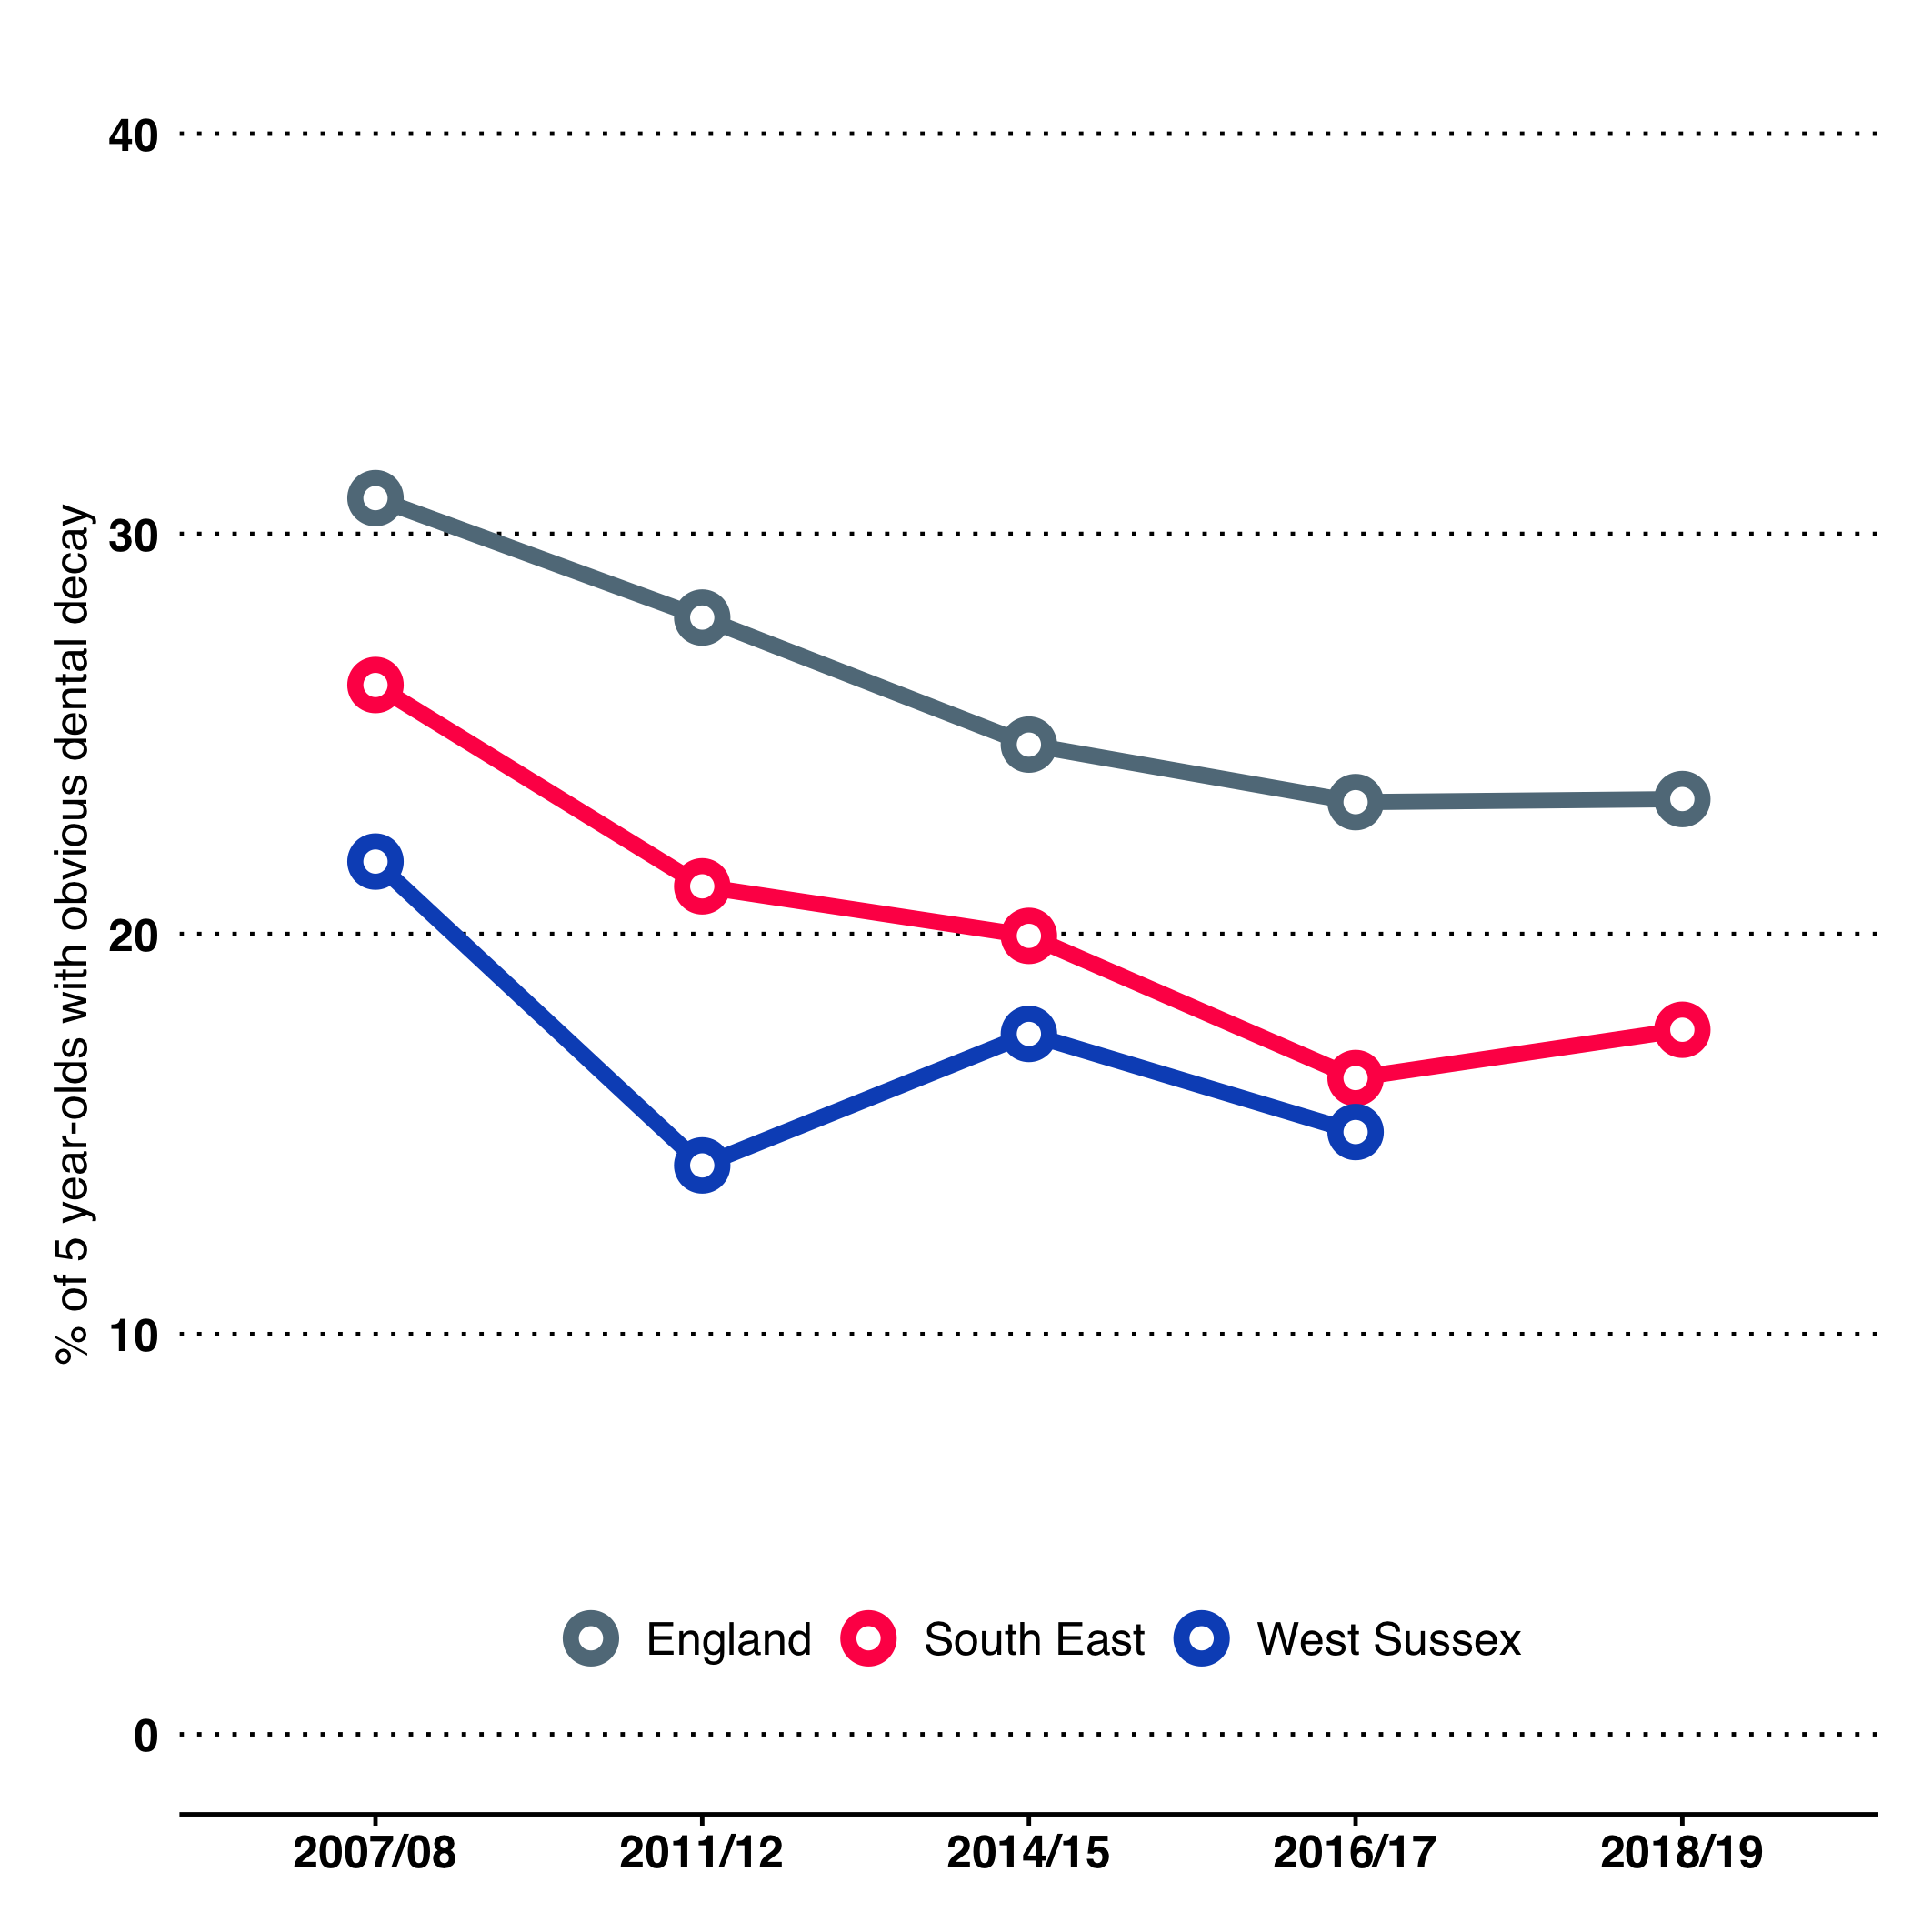
\includegraphics[width=\linewidth]{images/visual_dental_decay_5yos.png}
%	\label{fig:vodd_wsx}
%\end{figure}


%In 2016/17, dental services activity was greater overall than England, with the highest activity in Mid Sussex and the lowest in Chichester and Worthing.

%West Sussex children have a greater rate of "examinations" and "scale and polish" than nationally and lower rates of "permanent fillings and sealant restorations" in primary care, implying more check-ups help to prevent invasive treatments.

%Aside from using private dentistry, the most common reasons for not seeking a dental appointment in the last two years were residents not thinking they could get an NHS dentist and the belief they didn't need to see a dentist.

%\paragraph{Provision of dental services }
%In 2017/18, there were 146 dental contracts withinWest Sussex, covering general dentistry, community dental services and emergency access clinics. The required travelling distance is 10 miles or more for children living in some areas of Chichester district. 

%More children had seen a dentist (71\%, not including private dentists) than nationally in the 24 months prior to 2016/17. 

%Access rates were slightly better than England overall:
%\begin{itemize}
%    \item 6-12 year-olds had the highest rates, at 84.1\%
%    \item The 0-2 age group had the lowest rates, at 19.0\% vs. 21.7\% nationally. 
%\end{itemize}
 
%None of the districts in West Sussex fulfilled their NHS-contracted quota in 2016/17. Chichester, Arun, Mid Sussex and Worthing districts significantly underperformed.

%\subsubsection{Risk factors}
%More deprived local authorities have higher rates of dental decay (with the exception of Worthing), in line with the national pattern.

%Compared to England, West Sussex has a higher proportion of Special Educational Needs (SEN) children, who tend to have greater anxieties around seeing a dentist so are more at risk of poor oral health. Fewer SEN children had dental decay than nationally, although a higher percentage had substantial plaque compared to the South East region. 

%"Looked after" children are less likely to visit a dentist regularly and tend to have more dental disease and oral care neglect than those not in care. In West Sussex, a greater percentage of looked after children had seen the dentist than nationally (92.9\% vs. 84.4\%). 

\subsection{Health Related Behaviours and Healthy Weight}
\paragraph{Health-related behaviour of young people} 
Using the data from the 2014/15 national What About Youth (WAY) survey, 10.6\% of 15 year-olds in West Sussex stated that they were current smokers\footnote{The WAY survey data has been replaced by NHS Digital: Smoking, Drinking and Drug Use (SDD) in England as a PHOF indicator (previously 2.09i). However lack of local data in the SDD means the WAY survey remains the most recent estimate of smoking in young people in West Sussex.}. This is higher than England (8.2\%) and high amongst comparable authorities, although some caution is needed, given the lack of trend data and small sample sizes.

{\bfseries There were 195 hospital admissions for alcohol-specific conditions (of under 18s) in the period from 2018/19 to 2020/21. This is a rate of 36.9 per 100,000, which is significantly higher than the England rate of 29.3. These admissions have been increasing and are now at their highest level since 2011/12 to 2013/14, even as rates in England have fallen.}

The chlamydia detection rate \footnote{PHOF reference D02a.} remains below the England rate. In 2020, the rate was 1,003 per 100,000 15-24 year-olds and low compared with similar authorities.

West Sussex has a low teenage pregnancy rate\footnote{PHOF reference C02a.}, at 12.6 per 1,000 15-17 year-olds (179 conceptions) in 2019. This rate was slightly higher than in 2016 but remains low compared with England (rate of 15.7).

% Adur (rate of 14.8), Arun (18.9), Worthing (19.1) and Crawley (22.8) have rates similar to England.

{\bfseries The number of births to teenage mothers is less than a quarter of what it was ten years ago,} falling from 103 in 2010/2011 to 25 in 2020/21. 0.3\% of all births are to women in their teenage years. 

47.3\% of children aged 5-16 met the recommendations for physical activity in 2020/21\footnote{PHOF reference C10. The recommended physical activity is an average of at least 60 minutes moderate-vigorous intensity activity per day across the week.}, in line with England and national benchmark. The only lower tier authority in West Sussex with a sufficient sample size was Crawley, with 49.6\% of children which is also similar to the national figure.

\subsubsection{Healthy Weight - Reception and Year 6 Pupils}
In England in 2020/21, over a fifth of reception children were overweight or obese, increasing to over a third in Year 6. In West Sussex, the prevalence of obesity was lower than national levels, with 19.2\% of reception age children (4- 5 years old) and 28.8\% of Year 6 children (10-11 years old) measured as overweight or obese\footnote{PHOF references C09a and C09b.}.

% No lower tier data for 2020/21 at time of writing
% Within local authorities, the prevalence of overweight and obesity is varied. Arun, Worthing and Chichester had the highest prevalence of overweight and obesity among reception children (21.6\%, 21.5\% and 21.2\%, respectively) and Worthing had the highest prevalence among Year 6 children (32.3\%)

Inequalities in childhood obesity persist. For both school year groups, prevalence of excess weight among children living in the most deprived areas of West Sussex is greater than those living in the least deprived areas.

The Research Unit has drafted a briefing on data from the National Child Measurement Programme. This is available on the JSNA website.

\subsubsection{Education}
\paragraph{Early Years Provision, Education, NEET \& Progression to Higher Education}
Note: Unless stated, data for this section have been taken from the Department for Education Local authority interactive tool (LAIT). This is an interactive online tool. \url{https://www.gov.uk/government/publications/local-authority-interactive-tool-lait}

77\% of 2 year-olds in West Sussex benefited from funded early years (2 year-olds) in 2019. This is higher than the England rate and that of comparable authorities.

55\% of 2, 3 and 4 year-olds are in funded early provision with staff who have graduate status, similar to the England rate.

\paragraph{Special Educational Needs}

In January 2021 3.1\% of pupils attending a West Sussex school had a statement or Education, Health and Care (EHC) plan. This percentage is similar to regional and national percentages. The number of children on such plans has been increasing since 2018.

% There were 3,218 children with a moderate learning difficulty known to schools in 2018, and 348 with a severe learning disability.

As at 31 December 2021, 92.4\% of 16 and 17 year olds with SEN in West Sussex were in Education or Training. This is higher than both England and the average of the county's statistical neighbours.

\paragraph{16-17 year-olds not in education, employment or training (NEET)}

Compared to other authorities in the South East, West Sussex has the third highest proportion of 16-17 year-olds not in education, employment or training, at 7.7\% in 2020 (England 5.5\%, South East 6.4\%)\footnote{This is a West Sussex Plan priority. Refer the WSCC website for the latest data and commentary. The combined known and unknown status of NEET 16-17 year-olds is a PHOF indicator (B05).}. This represents 1320 young people in West Sussex.

Broken down, 5.5\% of this group has unknown status which, while lower than than in recent years is higher than both the average of statistical neighbours (3.4\%) and England (2.7\%). 

% (6.7\% of the total 16-17 year-old population). However, this portion of 16-17 year-olds has decreased, relative to 2016 figures, whilst the portion of NEET 16-17 year-olds with known status has increased (rising from 1.4\% to 2.4\% of the total 16-17 year-old population). 

\paragraph{School readiness} Overall, West Sussex compares poorly or similarly to the England level for school readiness measures\footnote{PHOF indicators B02a and B02b}, and performs significantly worse for children with free school meal status. West Sussex has been improving in recent years for these measures, however, and remains broadly comparable to statistical neighbours.

At Key Stage 2 (children aged 10-11 years), attainment is notably low, with 63\% of pupils achieving the expected standard in reading, writing and maths in 2019, and only 7\% of pupils attaining the higher standard (compared with 11\% nationally).

These figures have not been updated since the previous JSNA summary.

\begin{figure}[htp]
    \centering
    \caption{School readiness in West Sussex (2019)}
    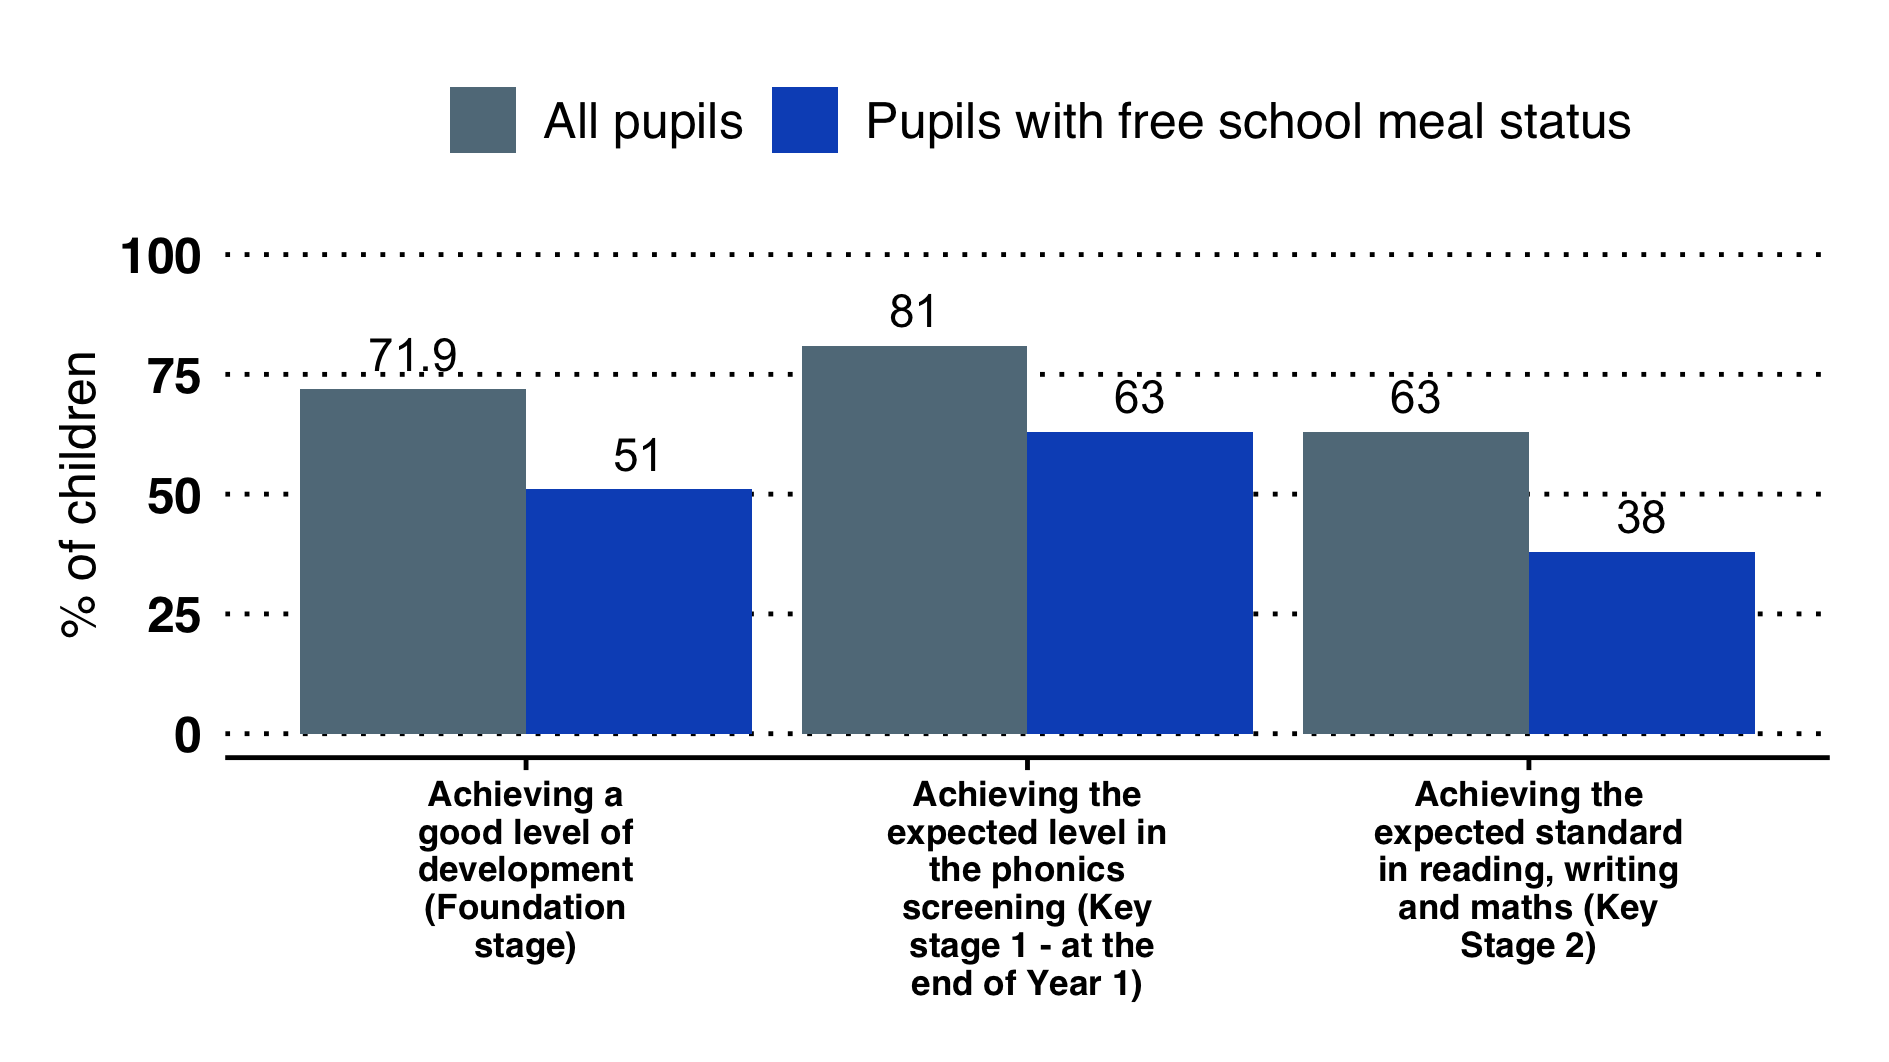
\includegraphics[width = \linewidth]{images/02_school_readiness_2019.png}
\end{figure}

At Key Stage 4 (GCSE level), attainment is above England overall (on the average P8 score measure) and in line with comparable authorities.

\paragraph{Progression to Higher Education (HE)} 40\% of all pupils progressed to higher education by age 19 in 2017/18, lower than England (43\%) and statistical neighbours (40.1\%). {\bfseries Significantly fewer pupils on free school meals progressed to HE, at 19\%} (England 27\%, statistical neighbours 16.5\%).

Data from the Office for Students shows some areas in West Sussex (including Littlehampton) are ranked in the lowest national quintile for progression to HE\footnote{Office for Students. POLAR - Participation of Local Areas. 2017.}.

\subsubsection{Social Care and Community Safety}
Note: Unless stated, data for this section have been taken from the Department for Education Local authority interactive tool (LAIT). This is an interactive online tool.\footnote{\url{https://www.gov.uk/government/publications/local-authority-interactive-tool-lait}}
\paragraph{Social Care and Criminal Justice}

As at 31 March 2021 there were 891 children looked after, a rate of 50 per 10,000. The rate in West Sussex remains lower than England, but similar to statistical neighbours. 80 children were unaccompanied asylum seeking children.

\paragraph{Outcomes for Children Looked After and Children Leaving Care}
In 2021, 8\% of care leavers were not in touch with the local authority. This was higher than England but similar to comparable local authorities. 31\% of children looked after are noted as "persistent absentees".

In relation to the emotional and mental wellbeing of children in care, in 2020/21, a higher percentage (50.6\%) of children in West Sussex were children with a 'cause for concern'\footnote{PHOF reference C12. Strengths and Difficulties Questionnaire (SDQ) scores come from the SDQ questionnaire, a survey required to be completed by for each child looked after aged 5 to 16 years. It has five sections (emotional difficulties; conduct problems; hyperactivity or inattention; friendships and peer groups; and positive behaviour) plus an "impact supplement" to assist in the prediction of emotional health problems. The questionnaire is completed by the child's main carer. A score of 0 to 13 is considered normal, 14 to 16 borderline, and 17 to 40 is a cause for concern.} (whereby they scored 17 or above on the Strengths and Difficulty questionnaire, which asks questions on a range of issues relating to emotional and mental wellbeing). This was significantly higher than England (36.8\%).

\paragraph{Criminal Justice}

First time entrants to the criminal justice system declined in the county, down to 74 per 1,000 10-17 year-olds in 2020, making the rate in West Sussex significantly lower than that of England (169.2) and the lowest in the South East (156.7).

\paragraph{Children in Need (CiN)} The Children in Need rate, as at 31 March 2021, was 330.0 per 10,000. This is lower than England but broadly in line with comparable authorities. As at March 2021, there were 5,853 children in need.

6.7\% of Children in Need had a recorded disability. This is much lower than the England rate of 12.7\%.

The rate (per 10,000) of referrals to social services increased year on year between 2014 and 2018, although it declined slightly in 2019 and 2020 to 516.0. This rate is similar to England but higher than comparable local authorities. In total there were 8,803 referrals.

Section 47 enquiries\footnote{This relates to enquiries where there is reasonable cause to suspect the child is suffering, or is likely to suffer significant harm. Local authorities carry out an assessment under section 47 of the Children Act 1989 to determine if steps are needed to safeguard the child. Where concerns are substantiated, and the child is judged to be at continuing risk, an initial child protection conference should be convened within 15 working days.} (started within year) remain fairly steady, at 188.8 per 10,000. This was higher than England and comparable authorities.

\paragraph{Children subject to a Child Protection Plan (CPP)} In 2021, the rate of children subject to a CPP was 53.8 per 10,000, higher than England and comparable authorities. The percentage of children who became subject to a CPP for a second or subsequent time held steady at approximately 25\%. This is higher than comparable authorities and England.

\subsubsection{Transition to Adult}
Some young people, including those in care and young people with health needs and disabilities, require additional support as they enter adulthood. Many young people will have on-going services and this can be a time of considerable anxiety.

National research shows disabled young people aged 16-24 are less satisfied with their lives than their peers. There is a tendency for support to fall away at key transition points as young people move from child to adult services.

Following transition from a residential school, young people may experience good access to frontline health and social services, but also very few opportunities to enter employment or further education; no additional improvements in communication, self-care or behaviours that challenge; a reduction in good support for behaviours that challenge and increased reliance on restrictive practices; limited access to specialist services; and living at distance from the family home.

% \subsubsection{Further information}
% This is a summary document. More detailed local analyses (alongside a whole host of national profiles!) are available, including the needs assessment and briefings highlighted below. If you have specific information requests please contact the team.

% Contacts in the West Sussex Public Health and Social Research Team for Starting Well:
% \begin{itemize}
%     \item Jacqueline Clay - jacqueline.clay@westsussex.gov.uk
%     \item Dr Verity Pinkney - verity. pinkney@westsussex.gov.uk
% \end{itemize}  % Starting well
\newpage
\section{Living Well}
\subsection{Summary}
Foundations and behaviours established in childhood and the wider determinants of health (such as education, housing, income and the natural and built environment) impact health and wellbeing in adulthood. In the past 10 years, the UK has experienced a considerable increase in people aged 65 years and over and can expect greater increases to come, as the sustained baby-boom of the late 1950s to mid-1960s starts to enter older age groups in the next 10-20 years.

Action to improve mid-life, so that people enter older age healthier and happier, becomes increasingly important. This is not just to reduce pressure on health and social care services, but to sustain the ability to work and overall economic productivity, as the age-dependency ratio increases.

Having a good job has been found to be good for physical and mental wellbeing. West Sussex has high employment rate, with over 79\% of 16-64 year-olds in employment, 4\% higher than the England rate. However, wage rates in part of the county are relatively low, when compared with regional and national rates. Large gaps also remain in the employment rates for people with health problems or long-term conditions and the wider population. In 2020/21 the employment gaps were:

\begin{itemize}[noitemsep]
    \item 9.9\% between those with a long-term health condition and the overall employment rate, statistically comparable to the England average
    \item a 78.6\% between adults with a learning disability and the overall employment rate, which is significantly greater than in England
    \item 68.7\% between those in contact with secondary mental health services and the overall employment rate.
\end{itemize}

Having access to good quality, affordable housing is also crucial to health. In West Sussex, as in many parts of the UK, there is increased pressure on housing and costs have risen. Although data are limited, the number of people sleeping rough continues to increase.\todo[inline]{needs a comment here about the effect of the pandemic on homelessness, both over lockdown and since Autumn 2020}

In recent years, improvements in healthy life expectancy have stalled, particularly in women, where healthy life expectancy was lower in the period of 2016-18 compared with 2009-2011 and continues to plateau. However, there are likely to be many complex and inter-related reasons for this.

Four behaviours (tobacco smoking, alcohol consumption, diet and physical activity) continue to have a considerable impact on physical and mental health. Increased clustering of these behaviours, notably amongst people from the most deprived communities, are acting to increase health inequalities. Tackling these behaviours requires a whole system approach, working at population, community and individual level.

\begin{itemize}[noitemsep]
    \item The overall smoking rate in West Sussex is 11.2\%. People in lower socio-economic groups are 3 times more likely to smoke, however.
    \item The rate of hospital admissions for alcohol-related conditions for women under 40 is significantly higher than England, with over 500 admissions in 2018/19.\todo[inline]{find this one}
    \item Over 60\% of adults are estimated to be overweight or obese.
    \item An estimated 21\% of adults are physically inactive, engaging in less than 30 minutes of physical activity per week.
\end{itemize}

Emotional and mental wellbeing is as important, and intrinsically linked, to physical wellbeing. 14\% of adults in West Sussex are estimated to have common mental health problems, such as anxiety or depression. Over 7,500 people in the county have a recorded severe mental illness such as schizophrenia, bipolar affective disorder and other psychoses.\todo[inline]{Check if this figure has been updated.}

\subsection{Life expectancy}
\subsubsection{Healthy Life Expectancy at birth} Healthy life expectancy is the number of years a person can expect to live in good health (i.e without a disability and not in poor health)\footnote{PHOF reference A01a}.

\begin{figure}[htp]
    \caption{Healthy Life Expectancy at birth}
    \centering
	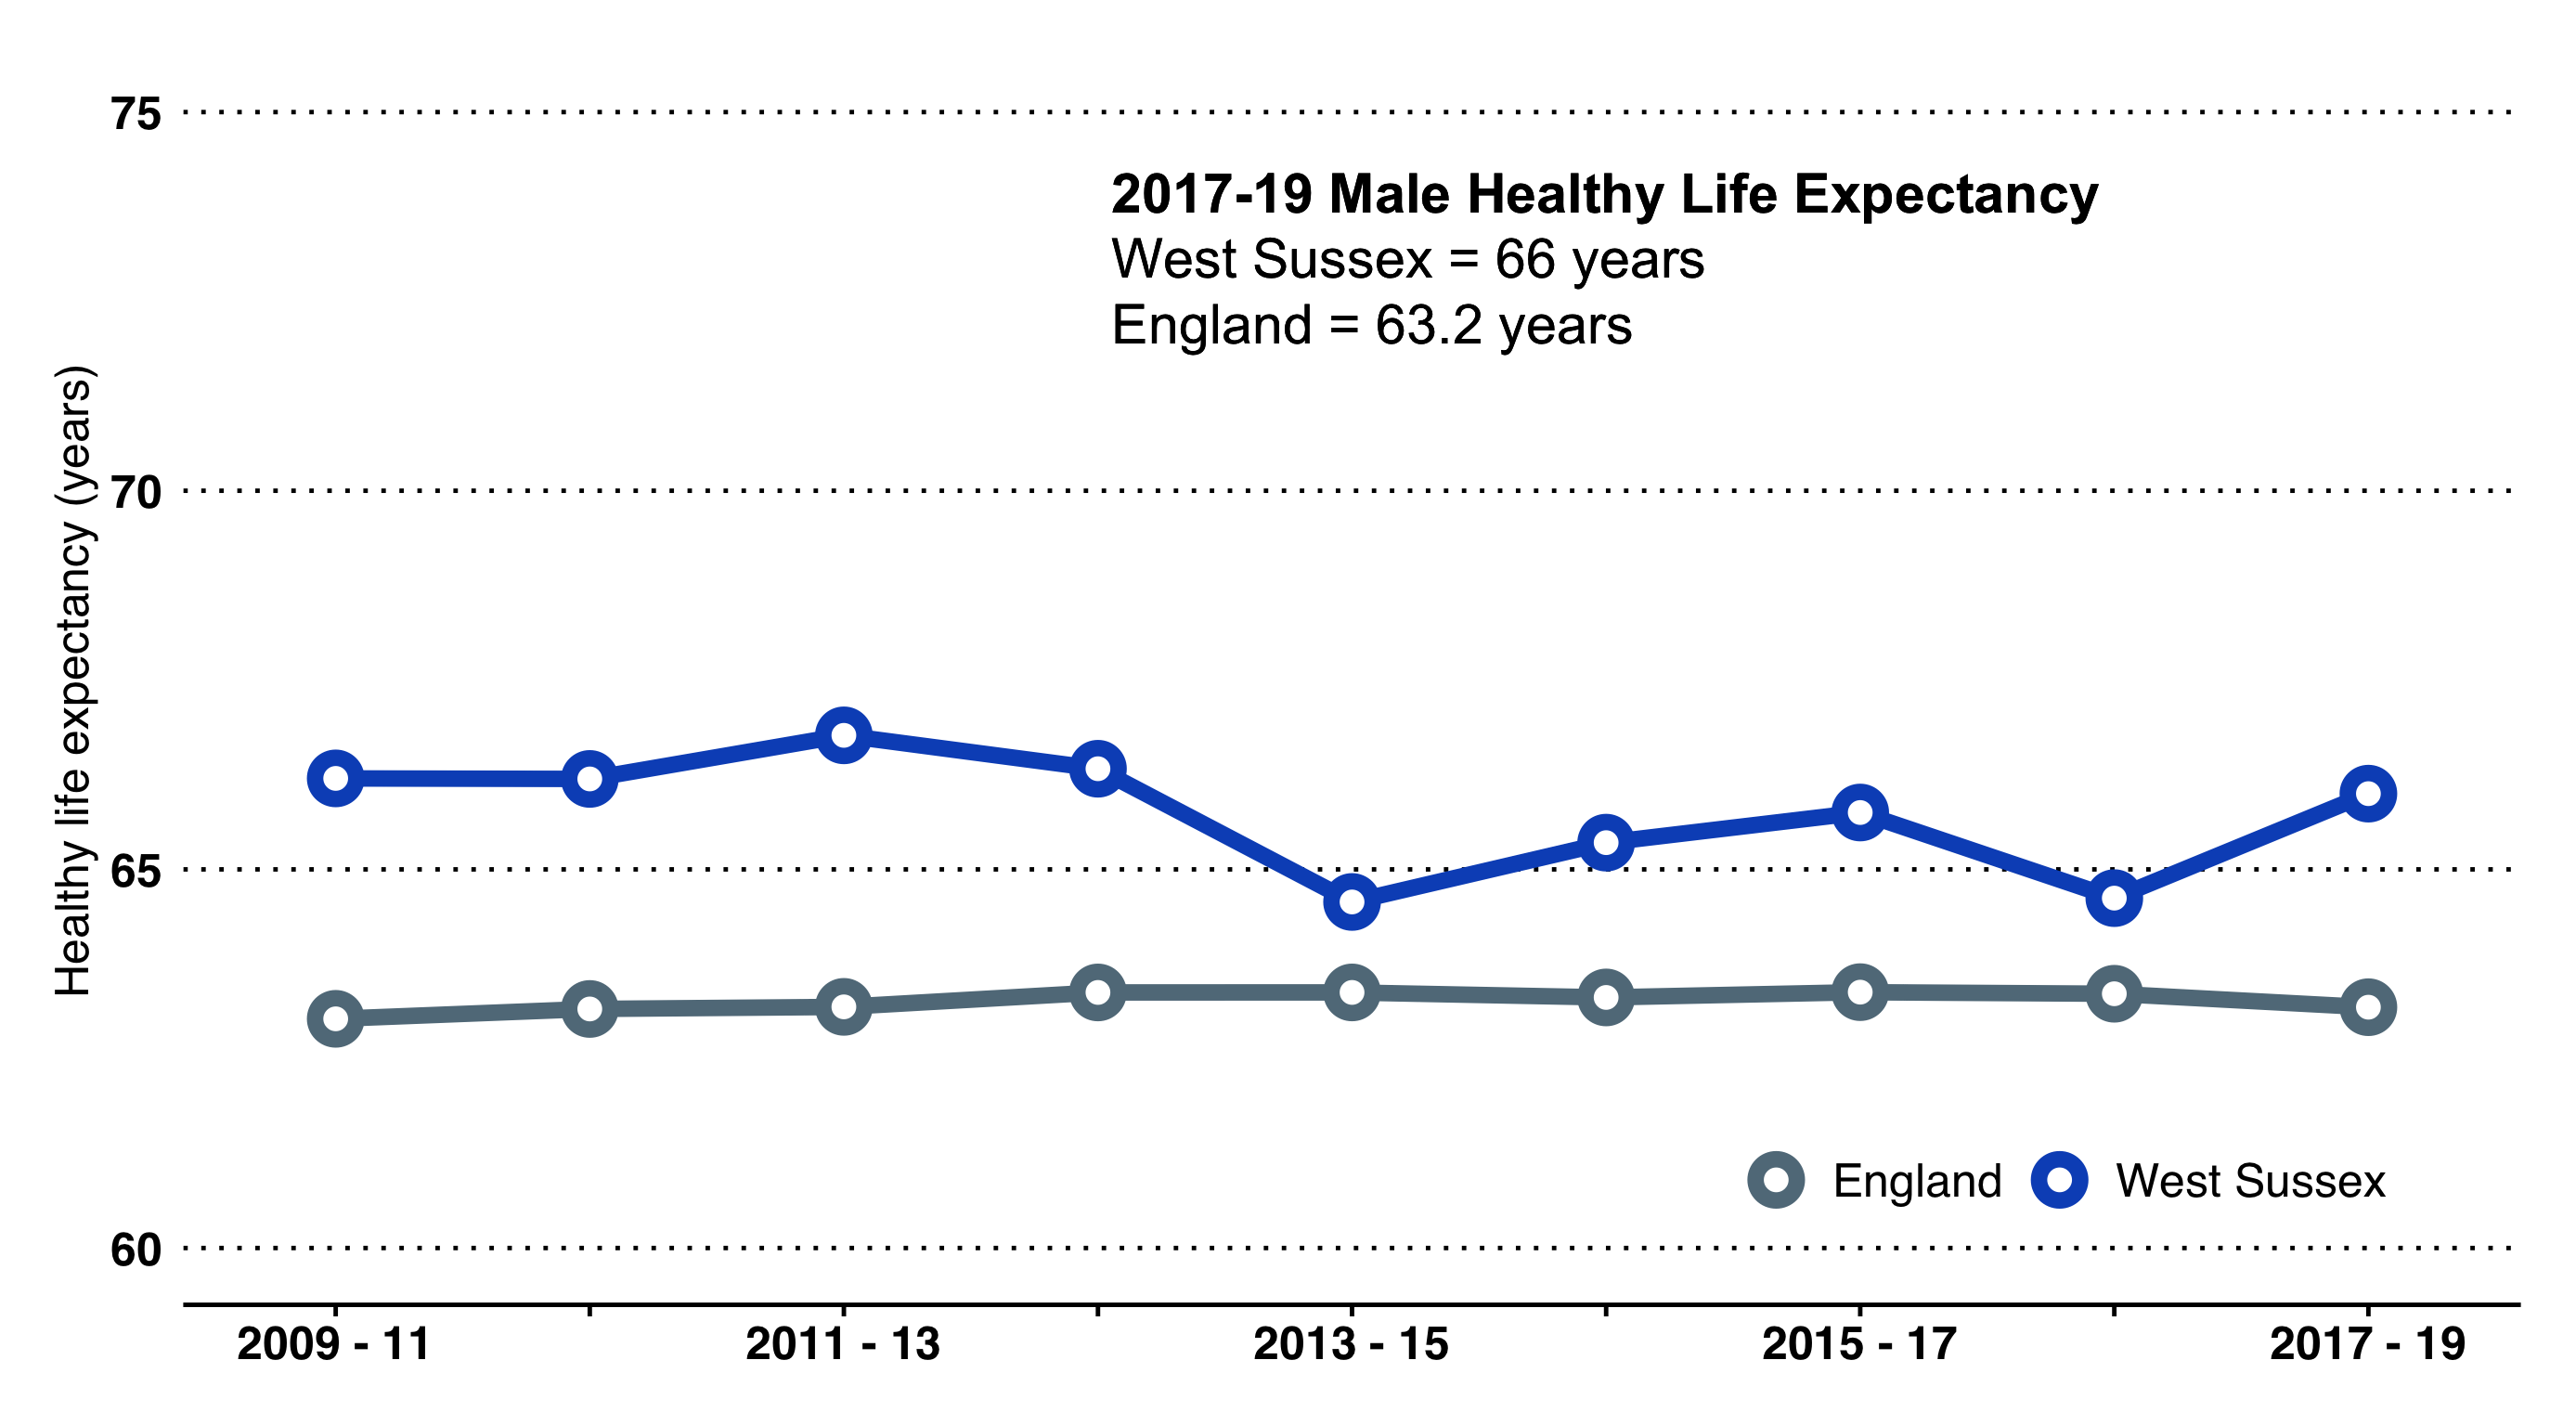
\includegraphics[width=\linewidth]{images/male_HLE.png}
    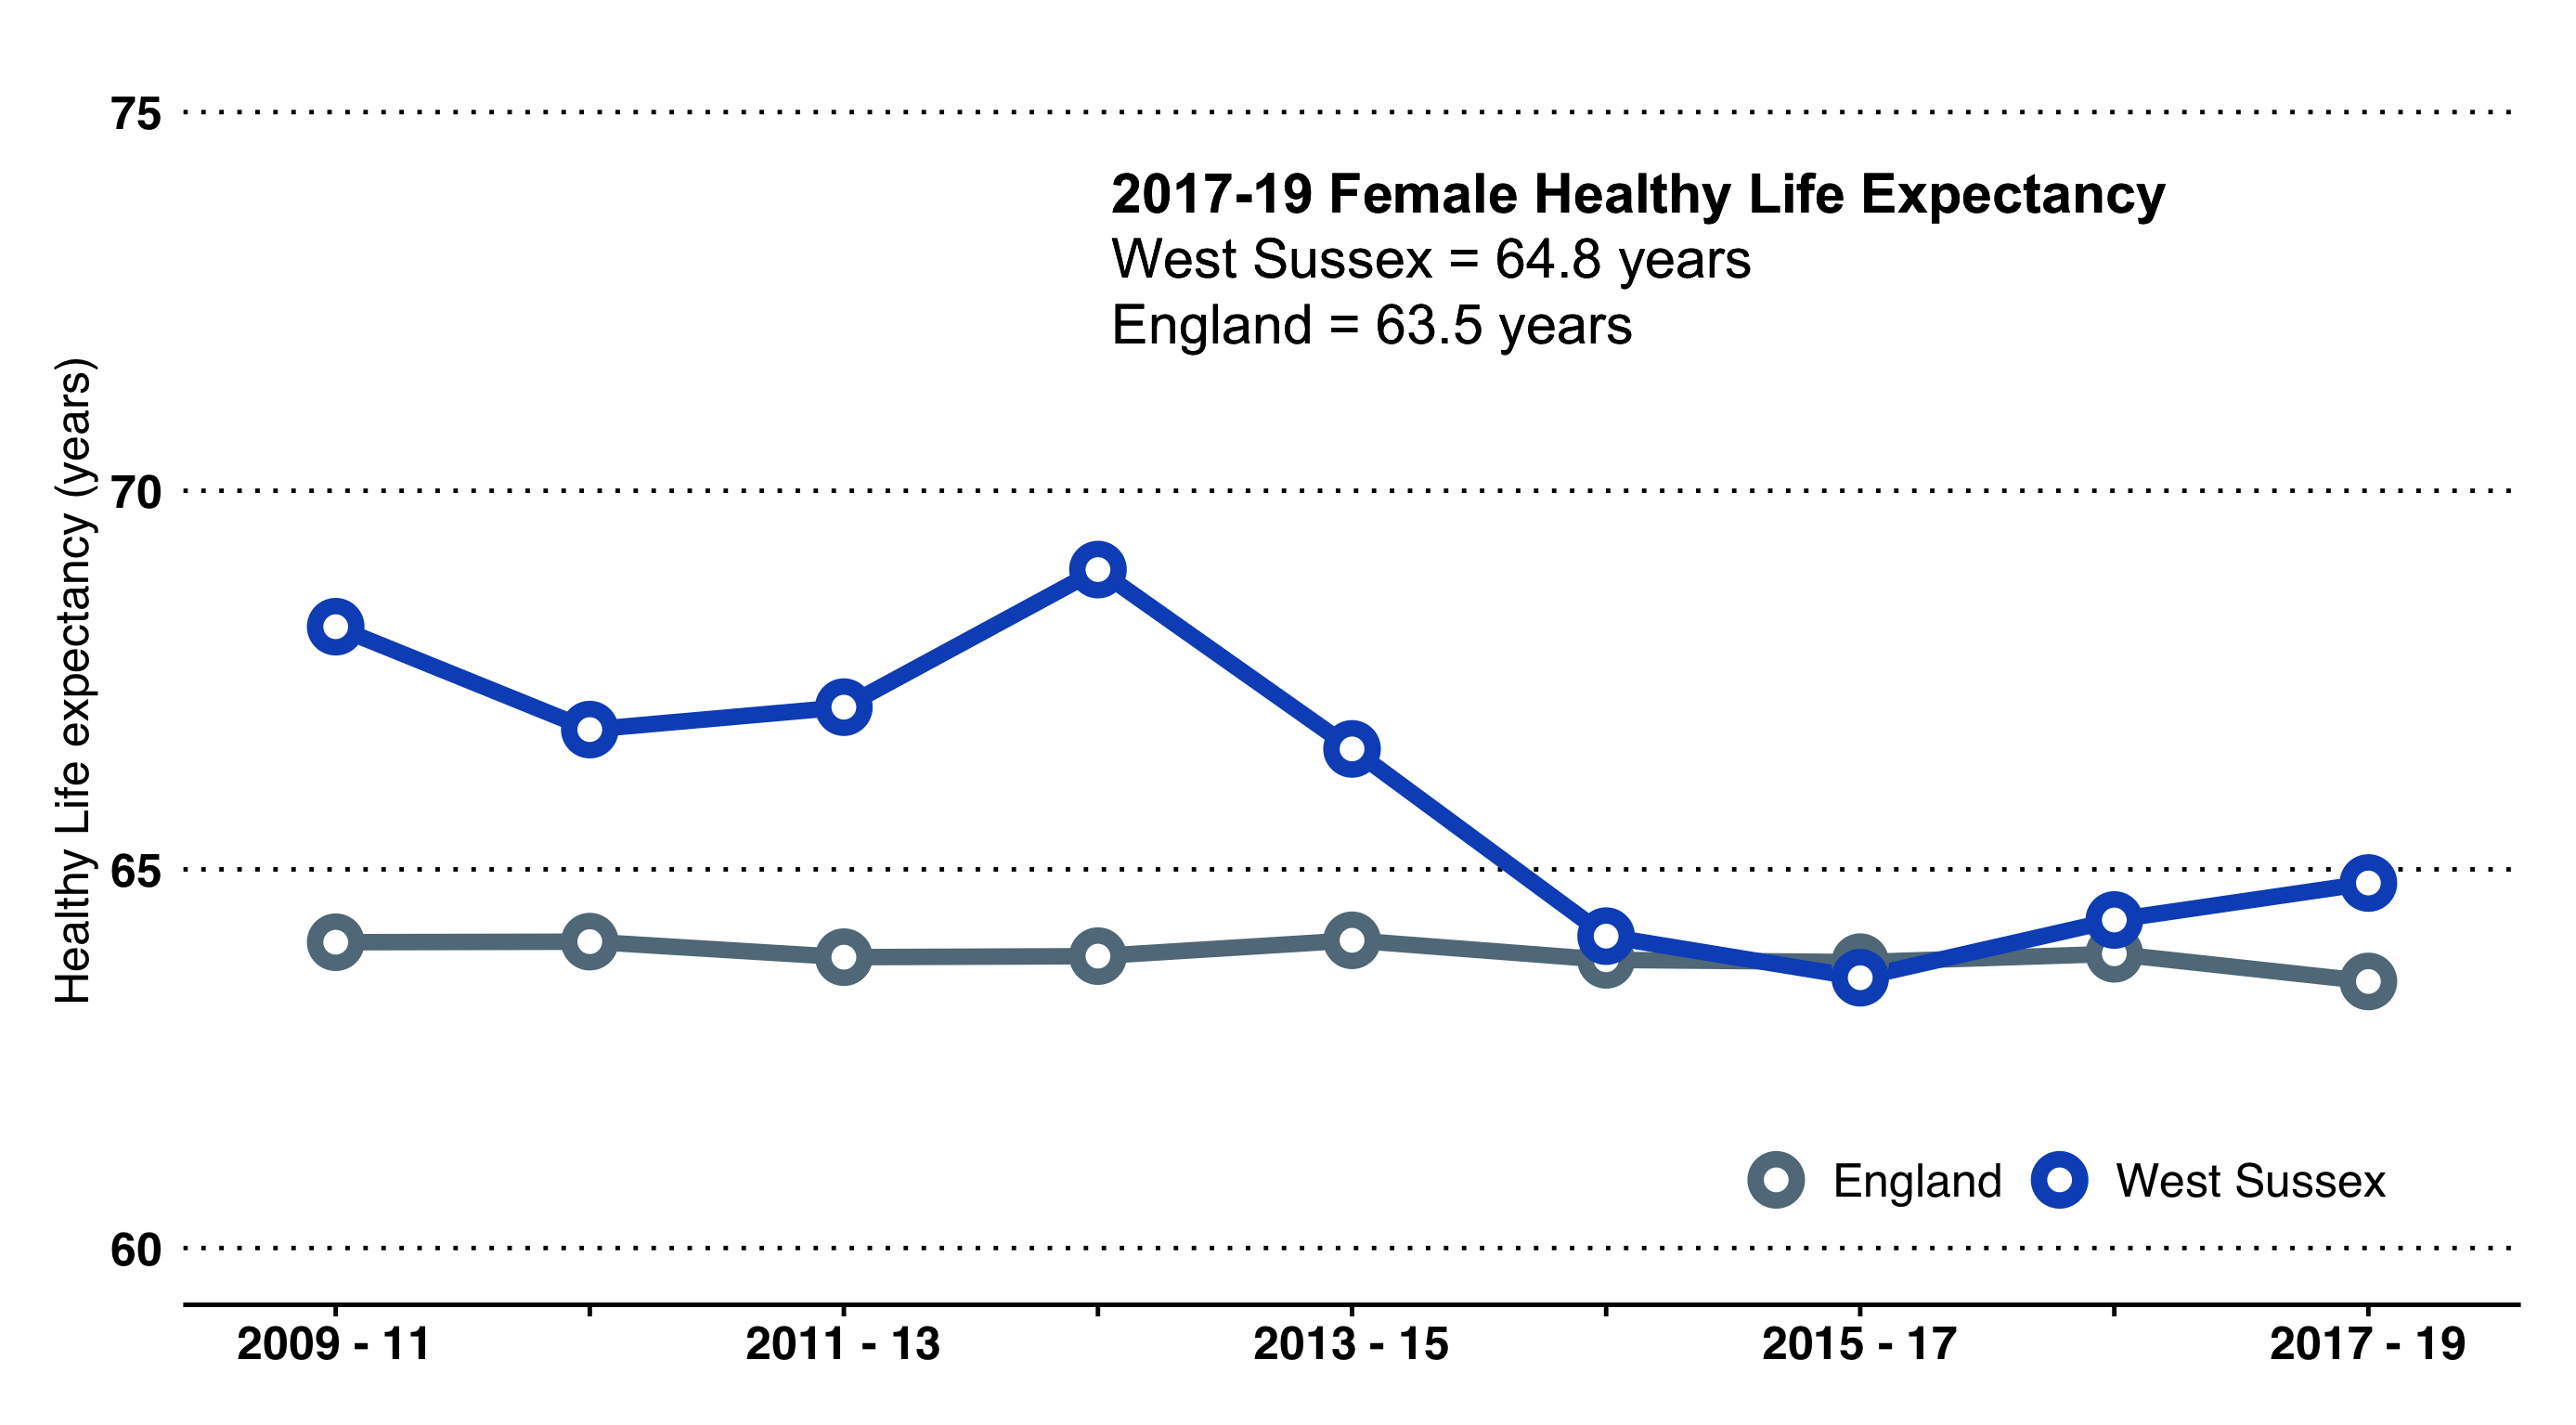
\includegraphics[width=\linewidth]{images/female_HLE.png}
	\label{fig:hle_wsx}
\end{figure}

Healthy life expectancies in West Sussex are comparable to England. In 2017-19, the male healthy life expectancy was 66.0 years and the female healthy life expectancy 64.8 years.

\paragraph{Female Life Expectancy - Changes between 2011-13 and 2017-19} Female healthy life expectancy has fallen considerably in recent years. In 2011-2013, West Sussex ranked 2nd amongst CIPFA comparators but by 2016-18 it had fallen to the second lowest amongst comparable local authorities. In the period 2017-19, West Sussex ranked 10th among comparable local authorities.

\begin{figure}[htp]
    \caption{Female Healthy Life Expectancy at birth - West Sussex compared to its statistical neighbours in 2009-11 and in 2017-19.}
    \centering
	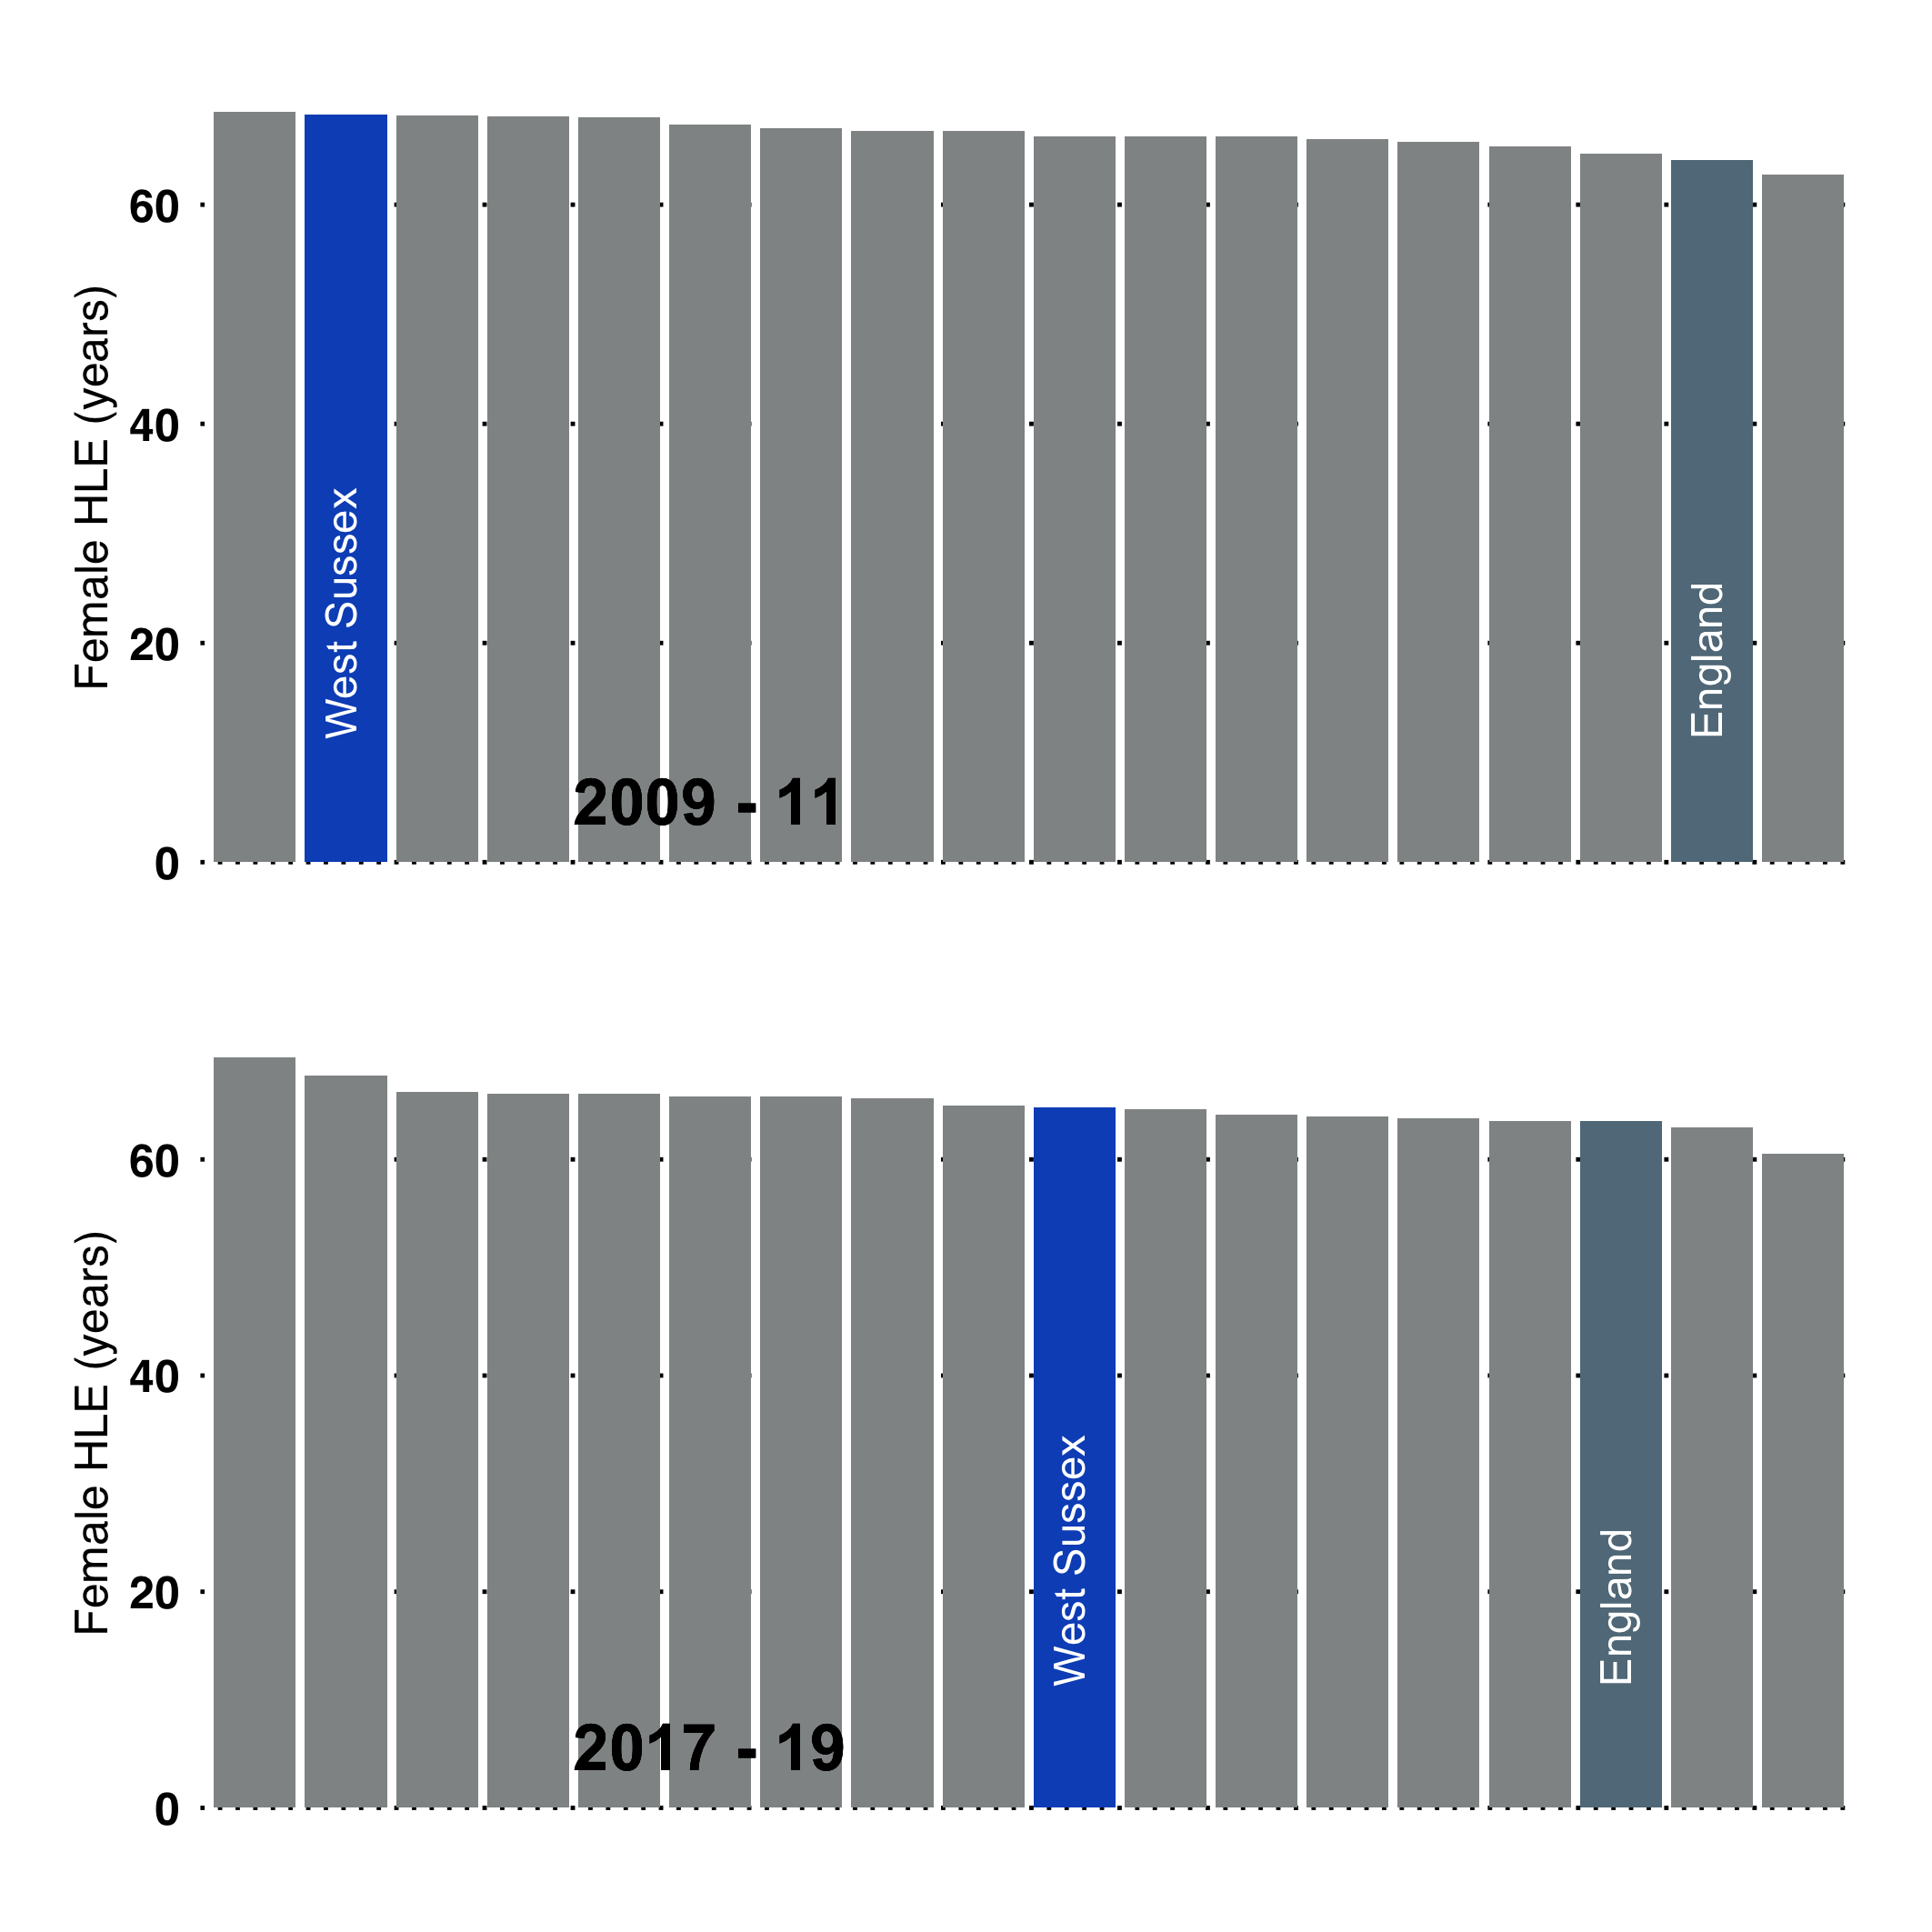
\includegraphics[width=.9\linewidth]{images/hle_cipfa.png}
	\label{fig:hle_cipfa}
\end{figure}

% \subsubsection{A Health Improvement Challenge} Improvements in health can secure considerable benefits.

\begin{tcolorbox}[width=\linewidth, title={A Health Improvement Challenge}, colback={boxcolour}]
As an example, NHS Choices details the benefits of regular activity. For adults aged over 18 years, 150 minutes of moderate activity or 75 minutes intense activity per week is recommended. Ideal moderate activity is brisk walking and cycling, which could be incorporated into active travel.

It is estimated that people who do regular physical activity have up to a:

\begin{itemize}[noitemsep]
    \item 35\% lower risk of coronary heart disease and stroke
    \item 50\% lower risk of type 2 diabetes
    \item 50\% lower risk of colon cancer
    \item 20\% lower risk of breast cancer
    \item 30\% lower risk of early death
    \item 83\% lower risk of osteoarthritis
    \item 68\% lower risk of hip fracture
    \item 30\% lower risk of falls (among older adults)
    \item 30\% lower risk of depression
    \item 30\% lower risk of dementia
\end{itemize}

For West Sussex, if all adults were physically active, this would translate to:

\begin{itemize}[noitemsep]
    \item 10,000 fewer people on coronary heart disease GP register
    \item 23,000 fewer people on diabetes GP register
    \item 20,000 fewer people on depression GP register
    \item 2,500 fewer people on dementia GP register
    \item 175 fewer cases of breast cancer per year
    \item 210 fewer cases of colon cancer per year
    \item 845 fewer emergency admissions for hip fracture in those aged 65 and over
\end{itemize}
\end{tcolorbox}

\subsection{Years of Potential Life Lost - West Sussex Primary Care Networks}
Years of Potential Life Lost (YPLL) is a measure of premature mortality.

If the average life expectancy in an area is 80 years and a death occurs at 50 we can describe the 30 year difference as "potential life years" lost to the population. By summing all the life years lost of people who have died prematurely we can calculate a summary for an area/group. People who die at a younger age contribute greater number of years; for example, a young person who dies at 20 in a car accident will have 60 years of life lost, whereas someone who dies at 72 would have 8 years of life lost. In using this measure, we look at the overall level of premature mortality (as a rate per 10,000 population) and at the cause of premature mortality so that we can identify the key causes of premature mortality.

For comparison with the previous JSNA summary, we  have again looked at deaths under the age of 75 by Primary Care Networks in West Sussex. We have summed the total years of life lost for deaths between 2017 and 2021 (5 years of data), calculated as a rate per PCN population aged under 75 years. (Figure~\ref{fig:ypll})

\begin{figure}[htp]
    \caption{Years of Potential Life Lost Rate per 10,000 Population (U75) Pooled Data of Deaths Registered Between 2017 and 2021.}
    \centering
	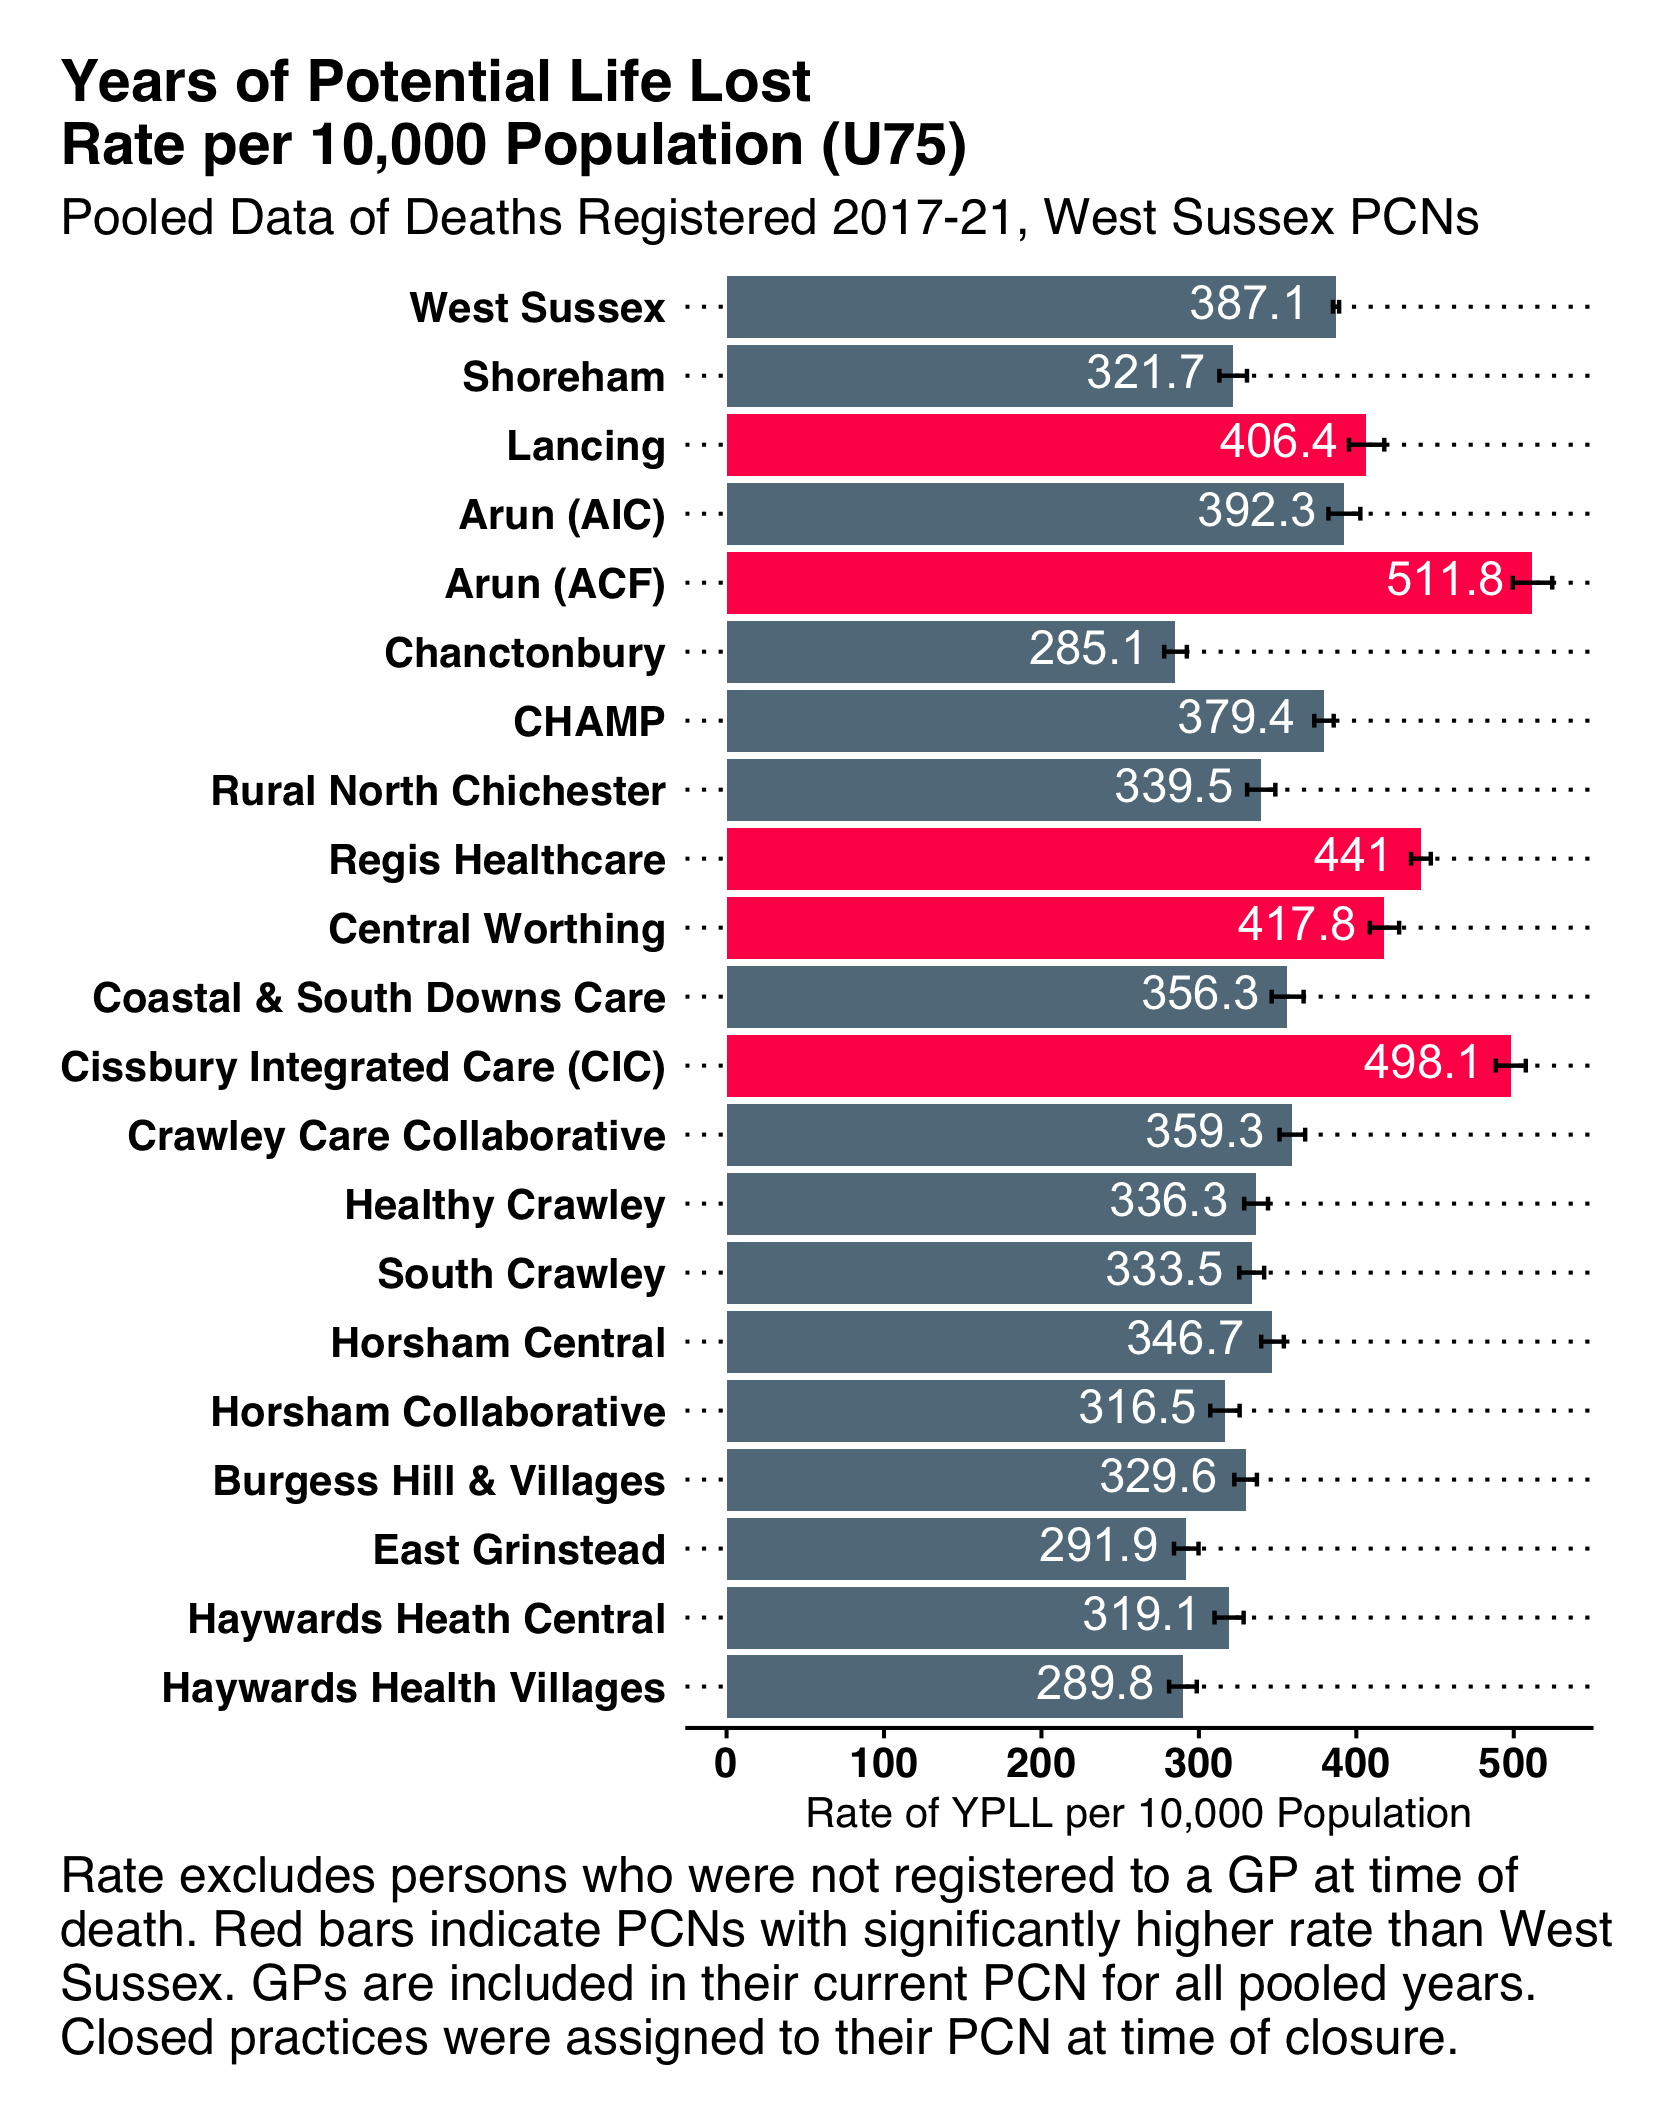
\includegraphics[width=\linewidth]{images/ypll_by_pcn.png}
	\label{fig:ypll}
\end{figure}

% https://www.healthknowledge.org.uk/public-health-textbook/research-methods/1a-epidemiology/years-lost-life

% Online, the source for this is OECD - might have been done by Rich last time?

Five PCNs have rates significantly higher compared with the West Sussex overall rate. These are Lancing, Arun (Neighbourhood 1), Regis (Neighbourhood I - Central Regis) and Cissbury. 

The top 5 causes of years of potential life lost are common across all the PCNs: cancer, diseases of the circulatory, respiratory and digestive systems, and external causes (such as accidents).

\subsection{Employment and Unemployment}
\paragraph{Economic Inactivity}
In West Sussex 92,900 people aged 16-64 years are estimated to be economically inactive (April 2020 to March 2021). Of these, over 68,500 are not seeking a job; with 16,000 people with long term sickness, 14,900 looking after the home or family, and 15,700 retired.

\paragraph{Long-term claimants of Jobseeker's Allowance}

The rate per 1,000 16-64 year-olds claiming Jobseeker' Allowance long-term (i.e. for more than 12 months) has improved in West Sussex in recent years, decreasing from 4.9 per 1,000 in 2012 to 1.8 per 1,000 in 2018 (a decrease of 1,455 people in this time period). The West Sussex rate is in line with CIPFA neighbours and below England (3.8 per 1,000 in 2018).

\begin{figure}[htp]
    \caption{Long-term claimants of Jobseeker' Allowance by West Sussex Local Authorities, 2020}\label{fig:longterm_jsa}
    \centering
	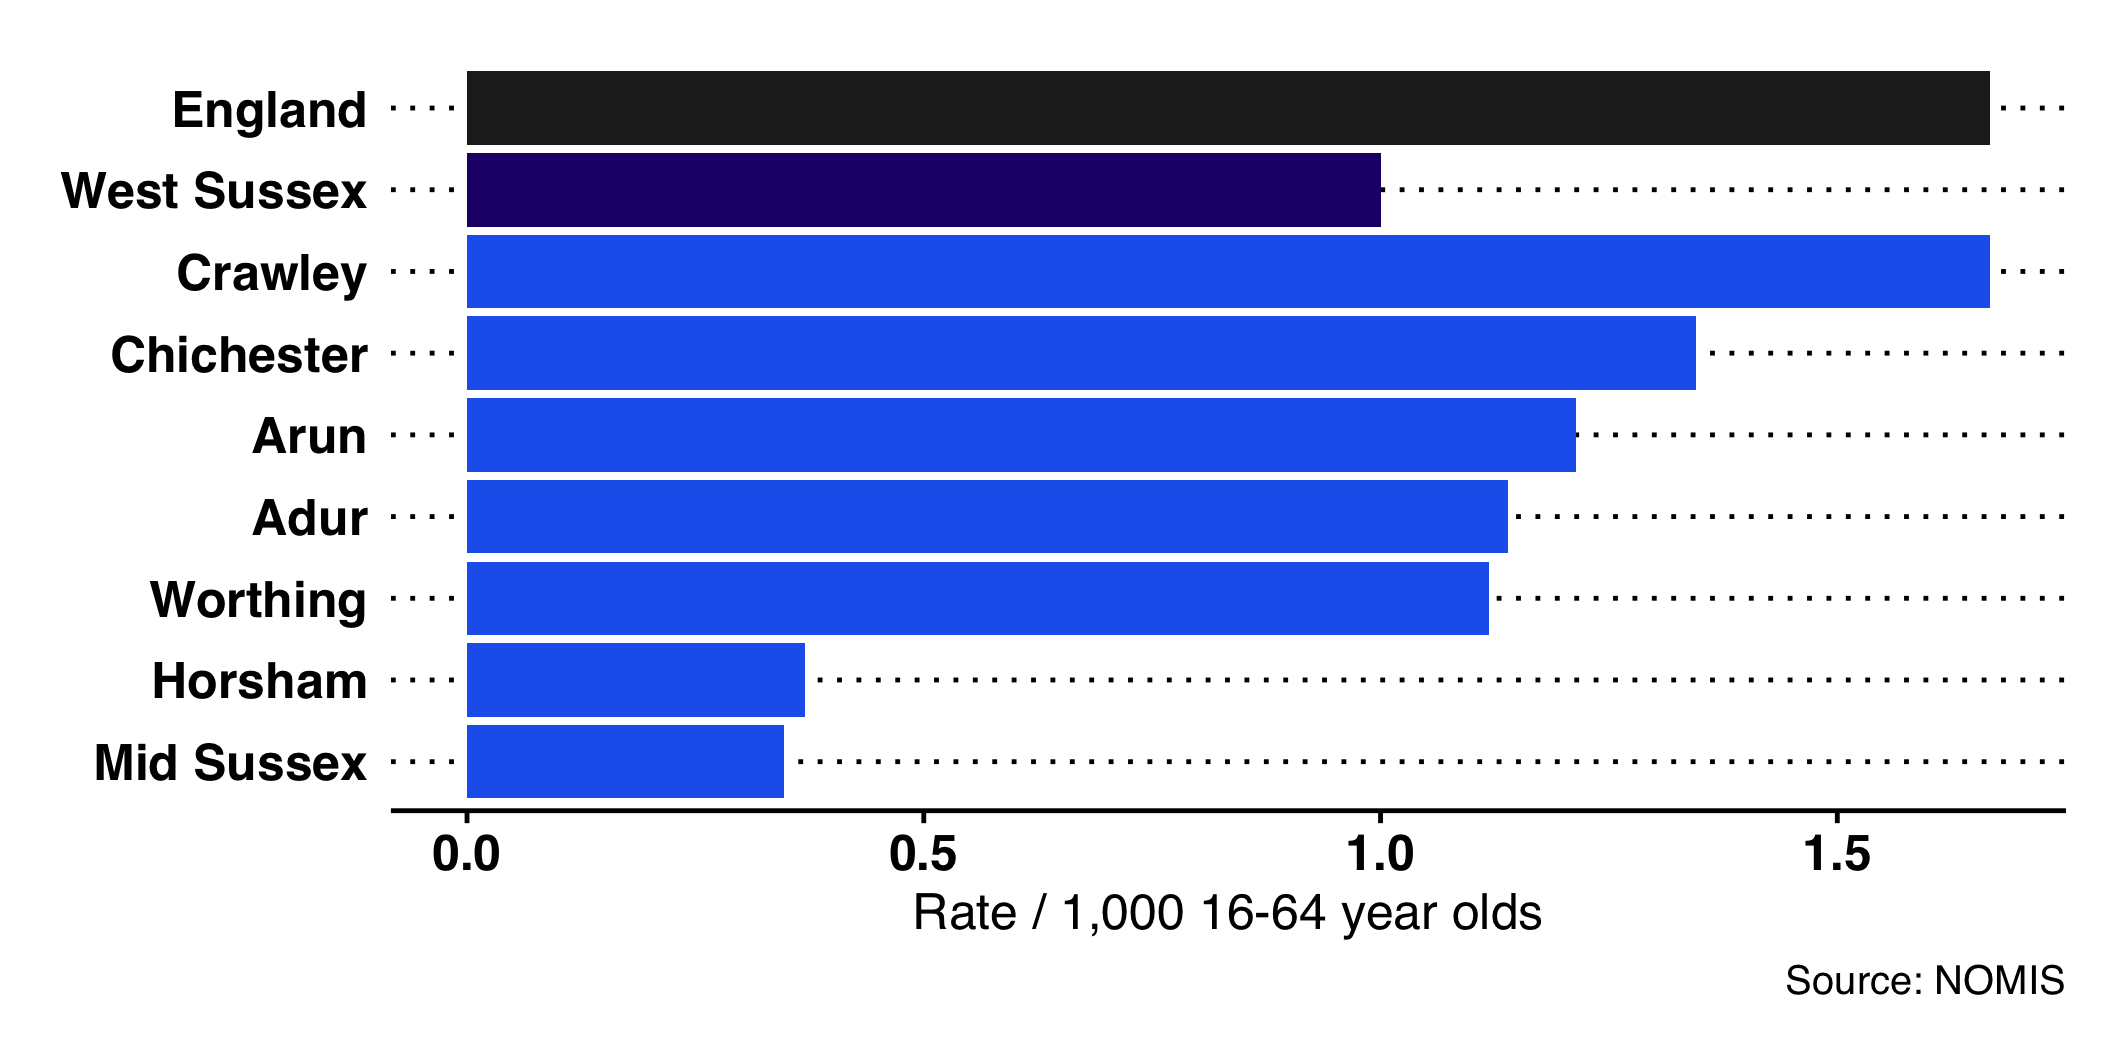
\includegraphics[width=.9\linewidth]{images/longterm_jsa_claimants_wsx.png}
\end{figure}

\paragraph{Out-Of-Work Benefits} In West Sussex, there are a similar proportion of claimants to the South East region as a whole (3.2\% compared to 3.3\%), this was approximately 16,300 people in March 2022. The number of claimants was significantly higher during the first Covid lockdown (at a peak of 27,500 in May 2020) but has been falling since.\footnote{Under Universal Credit a broader span of claimants are required to look for work than under Jobseeker's Allowance. As Universal Credit Full Service is rolled out in particular areas, the number of people recorded as being on the Claimant Count is therefore likely to rise.}

The Claimant Count is the number of people claiming benefit principally for the reason of being unemployed. This is measured by combining the number of people claiming Jobseeker's Allowance (JSA) and National Insurance credits with the number of people receiving Universal Credit principally for the reason of being unemployed. Claimants declare that they are out of work, capable of, available for and actively seeking work during the week in which the claim is made. Note that the Claimant Count is currently designated as an experimental statistic.

\paragraph{Employment Rate Gap of Vulnerable Groups}

The employment rate gap looks at the difference in the percentage of people who are part of a vulnerable group who are employed, compared to the percentage of all respondents in the Labour Force Survey classed as employed (aged 16-64)\footnote{PHOF references B08a, B08b and B08c.}.

In 2019/20, the employment rate gap for people with learning disability was significantly greater in West Sussex (78.6\%) compared to the overall rate across England (70.6\%).

In 2019/20, for both people with a long-term health condition, and people in contact with secondary mental health services, the employment rate gaps were similar in West Sussex compared with the overall rates across England.

The rate gap for people with a long term health condition has improved, decreasing from 14.3\% in 2018/19 to 9.9\% in 2019/20, similar to the England rate (67.2\%)\footnote{PHOF references B08a, B08b and B08c.}.

The rate gap for people in contact with secondary mental health services has remained at a similar level, decreasing from 69.1\% in 2018/19 to 68.7\% in 2019/20, similar to the England rate (67.2\%).

% This figure isn't great (as at 16/6), text renders too small on the labels. Current idea is to fill the bars with the text for the two longer bars? I'm still not that great at annotating plots outside the data ranges...

\begin{figure}[htp]
    \caption[Gaps in employment rate, West Sussex 2019/20.]{Gaps in employment rate for people with long term health conditions, people in contact with secondary mental health services, and people with learning disabilities. West Sussex, 2019/20.}\label{fig:emp_gaps}
    \centering
	
\includegraphics[width=.9\linewidth]{images/employment_gaps.png}
\end{figure}

\paragraph{Employment Deprived} As part of the Index of Deprivation 2019, the employment domain provides information on the proportion of the working age population in an area that are involuntarily excluded from the labour market. These are people who would like to work but are unable to, including those unemployed, ill, disabled or who have caring responsibilities.

\begin{table}[hbt]
    \caption{The proportion of working age population in West Sussex local authorities that are involuntarily excluded from the labour market. The England rate is 9.9\%.}
    \centering
    \begin{tabular}{lrr}
    \toprule
    \ & Number & Percentage \\
    \midrule
    Adur & 3,100 & 8.9 \\
    Arun & 7,000 & 9.0 \\
    Chichester & 3,900 & 6.4\\
    Crawley & 5,200 & 7.7\\
    Horsham & 3,800 & 5.1\\
    Mid Sussex & 3,700 & 4.6\\
    Worthing & 5,400 & 9.0\\
    West Sussex & 32,100 & 7.0\\
    \bottomrule
    \end{tabular}
    \label{tab:wa:empdep}
\end{table}

\subsubsection{Health and Social Care Workforce - Primary Care}
\paragraph{Primary Care Staffing} By West Sussex Clinical Commissioning Group (CCG). Data are estimated provided as of March 2022 by NHS Digital.\footnote{Note that direct patient care staff includes therapists, health care assistant, social prescribing link workers etc. FTE = Full Time Equivalent.}
% NB - might have three columns here staff type, FTE, head count
\begin{table}[hbt]
    \caption[Primary Care Staffing in NHS West Sussex CCG, March 2022.]{Primary Care Staffing in NHS West Sussex CCG, March 2022.}
    \centering
    \begin{tabular}{lrr}
    \toprule
    Staff Role & FTE & Headcount \\
    \midrule
    All GPs  & 474 & 647  \\
    Fully qualified GPs \scriptsize{(excludes Registrars)} & 575 & 404 \\
    Qualified permanent GPs \scriptsize{(excludes Registrars and Locums)} & 567 & 400 \\
    Nurses & 340 & 230 \\
    Direct patient care staff & 350 & 233 \\
    Admin / non-clinical staff & 1572 & 1090 \\
    \bottomrule
    \end{tabular}
    \label{tab:wa:primarystaff}
\end{table}

\todo[inline]{Find where I put the data on GPs aged 55+}

\begin{table}[hbt]
    \caption{Percentage of GPs Aged 55 or Over by West Sussex CCGs.}
    \centering
    \begin{tabular}{lrrrr}
    \toprule
    \ CWS & Craw & HMS & England \\
    \midrule
    \% GPs Over 55 & 17.9 & 25.3 & 16.1 & 19.5 \\
    \bottomrule
    \end{tabular}
    \label{tab:wa:primarystaff_o55}
\end{table}

% Will compare all staff roles in a new version of this chart
% FIGURES Staffing (FTE) per 100,000 Population -> GPs / Nurses / Direct Care Staff / Admin and non-clinical\footnote{CWS = Coastal West Sussex CCG, Craw = Crawley CCG, HMS = Horsham and Mid Sussex CCG}

\subsection{Health and Social Care Workforce - Social Care / Care Benefits}
Data from Skills for Care\footnote{\url{https://www.skillsforcare.org.uk/adult-social-care-workforce-data/Workforce-intelligence/Home.aspx}}
\begin{itemize}[noitemsep]
    \item Adult Social Care Workforce Data Set (ASC-WDS) (as at September 2018)
    \item Independent sector employees as at March 2019
\end{itemize}

\begin{figure}[h]
    \centering
    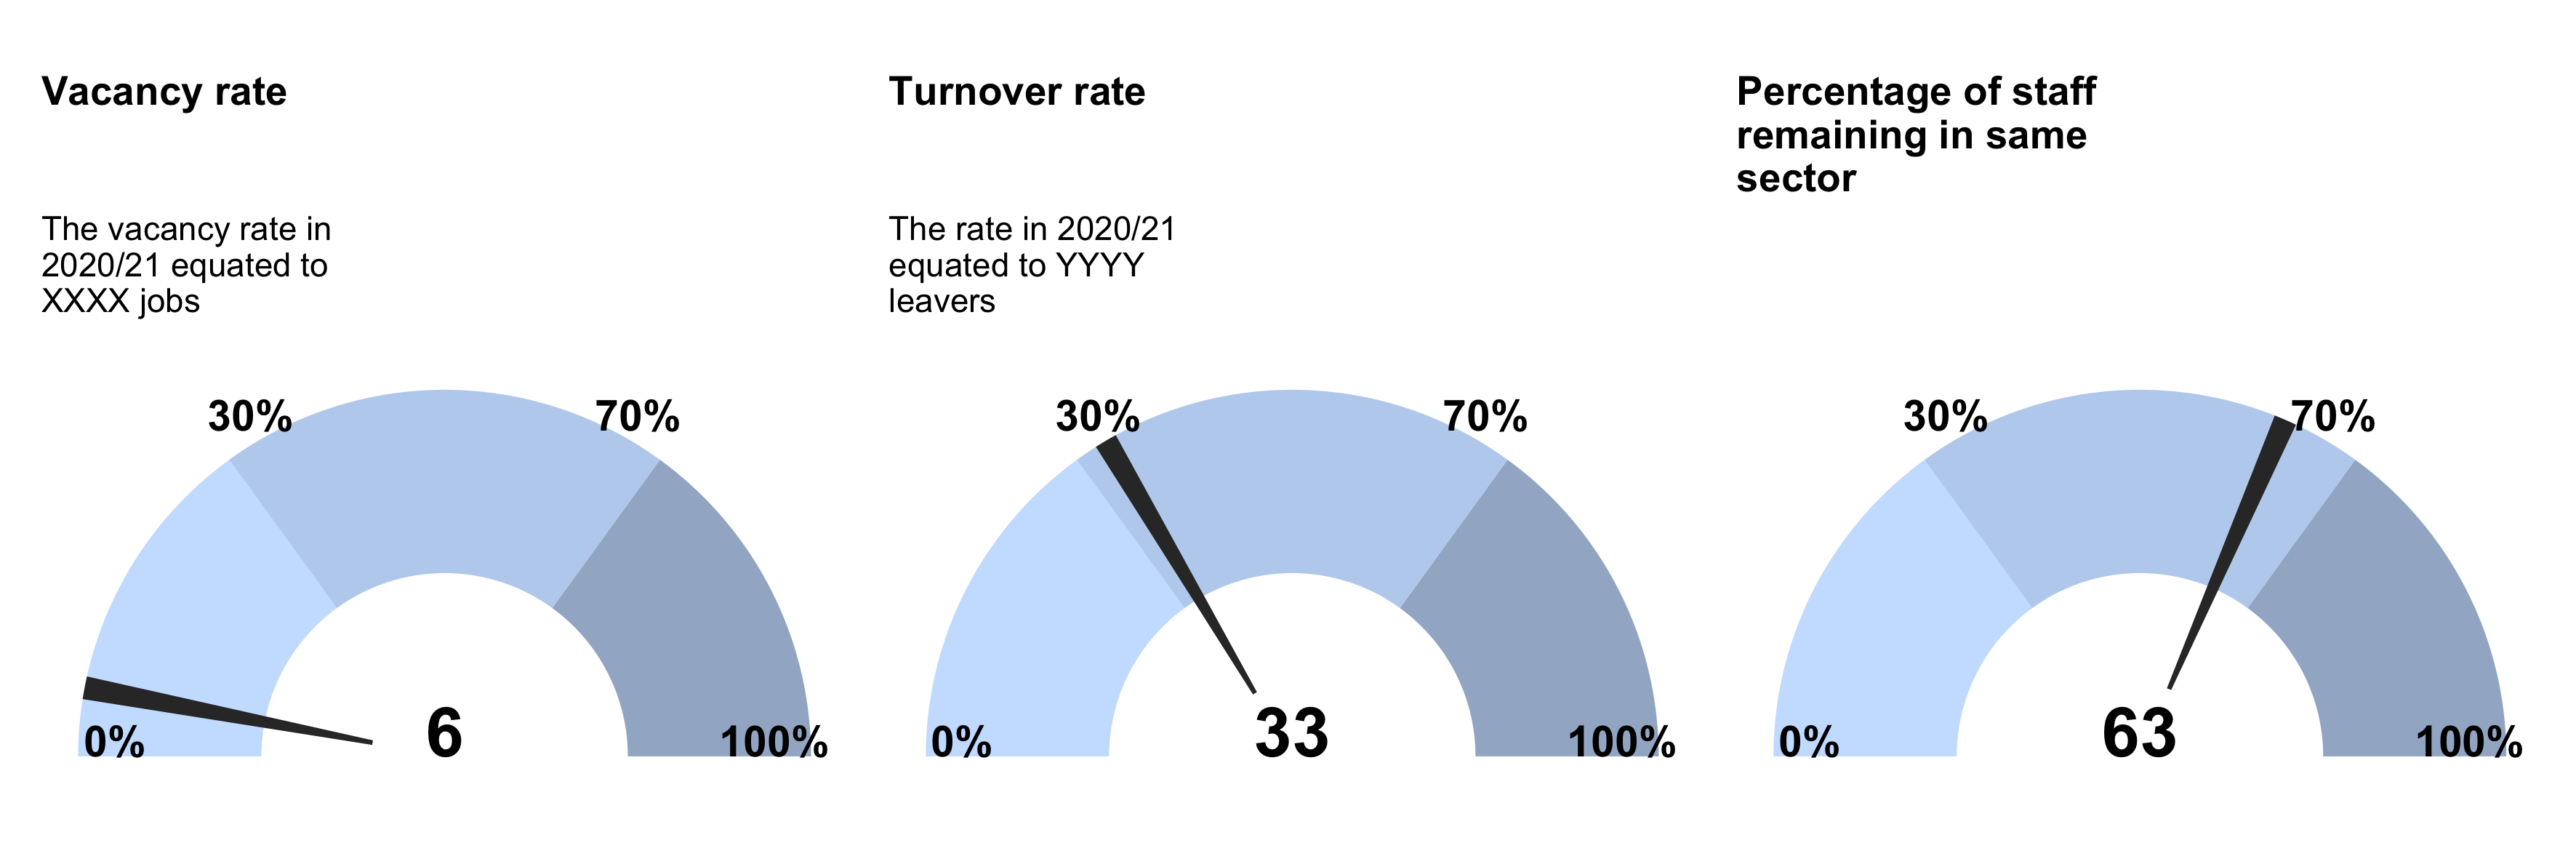
\includegraphics[width=\linewidth]{images/workforce_dial_chart.png}
\end{figure}

\begin{itemize}[noitemsep]
    \item Vacancy rate - The vacancy rate in 2018/19 equated to 2,100 jobs - 9\%
    \item Turnover Rate - The rate in 2018/19 equated to 6,900 leavers - 32\%
    \item Percentage of staff remaining in same sector - 66\%
\end{itemize} 

\begin{figure}[h]
    \caption{Estimated Number of Social Care Staff (all sectors)}\label{fig:sc-workforce}
    \centering
    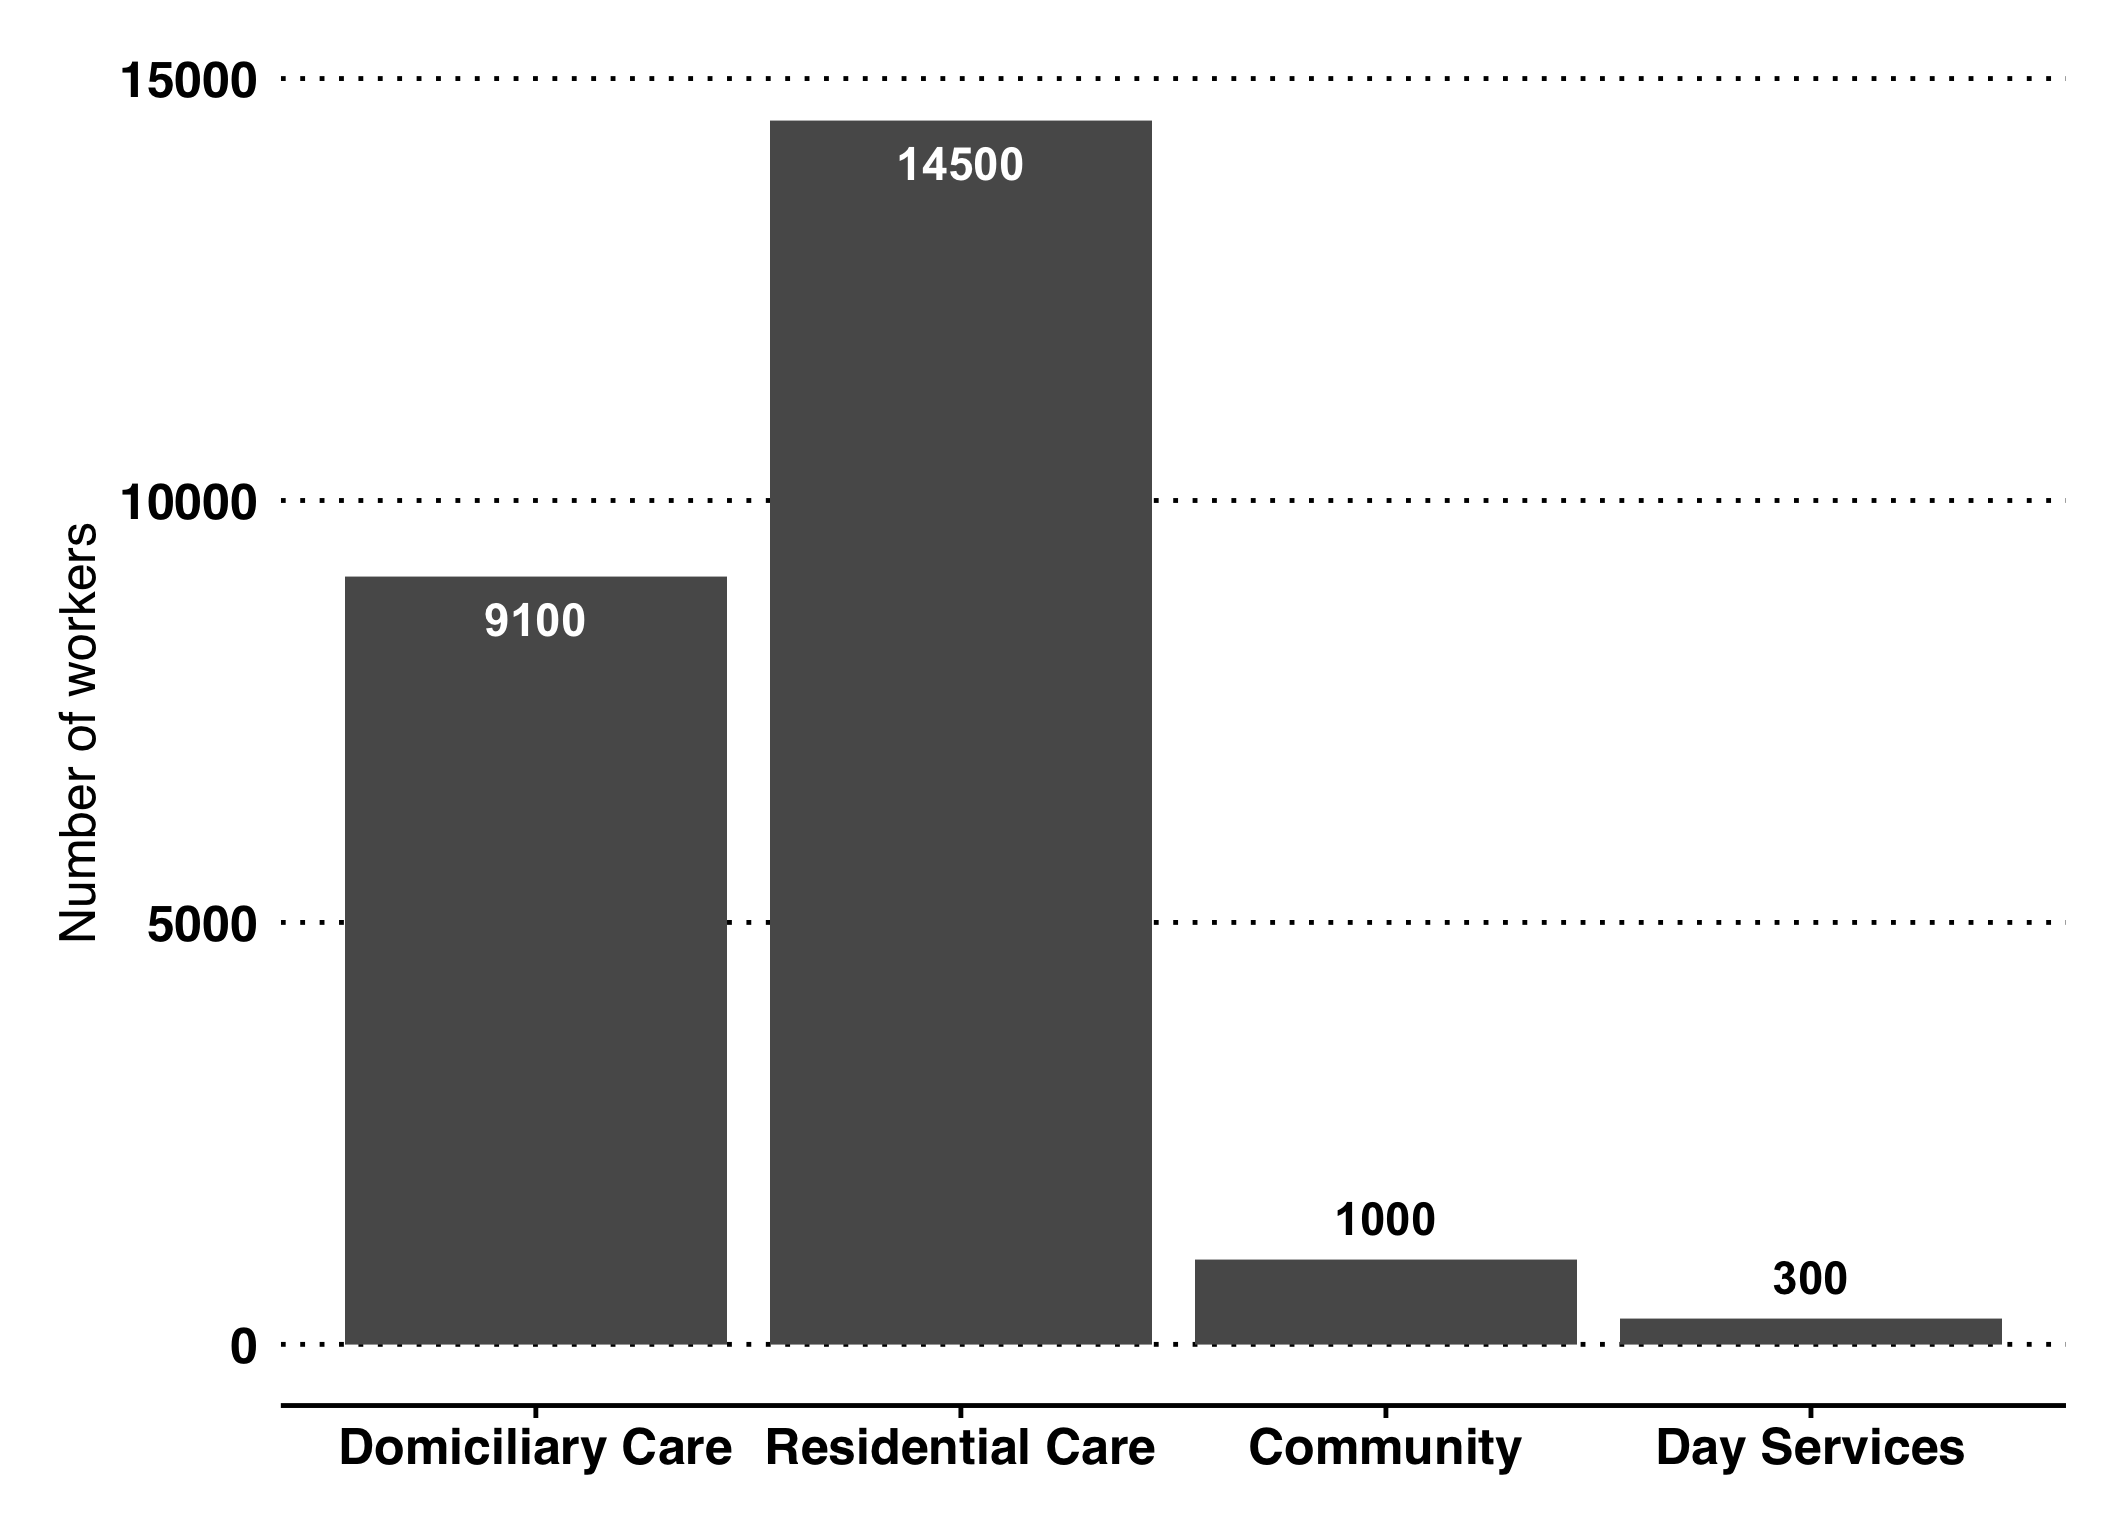
\includegraphics[width = \linewidth]{images/03-sc-workforce.png}
\end{figure}

\begin{itemize}[noitemsep]
    \item 27\% of workers are over 55
    \item Average Age = 44
    \item 82\% female
    \item 23\% of workers on zero hours contracts
    \item On average 8.8 days of sickness per year
\end{itemize}
   
\paragraph{Attendance Allowance - May 2019 (Rounded to nearest 10)} Attendance Allowance (AA) is non-means tested contribution towards additional costs incurred by people who have a disability and are aged 65 years or over. To qualify, people need to require help with personal care for at least 6 months. Payments are made at two rates: the lower rate (for people who need frequent help or constant supervision during the day, or supervision at night) and the higher rate (for people who need help or supervision throughout both day and night, or who are terminally ill).

\begin{table}[hbt]
    \caption{Attendance Allowance - November 2021}
    \centering
    \begin{tabular}{llll}
    \toprule
    \ & Total (People) & On Lower Rate & On Higher Rate \\
    \midrule
    Adur & 1790 & 740 & 1050 \\
    Arun & 5370 & 2090 & 3290 \\
    Chichester & 3310 & 1220 & 2100 \\
    Crawley & 1840 & 800 & 1040 \\
    Horsham & 3200 & 1310 & 1890 \\
    Mid Sussex & 2920 & 1250 & 1680 \\
    Worthing & 2930 & 1190 & 1740 \\
    West Sussex & 21360 & 8590 & 12780 \\
    \bottomrule
    \end{tabular}
    \label{tab:wa:att_all}
\end{table}



\paragraph{Carers Allowance - November 2021 (Rounded to nearest 10)} This is paid to people (aged 16 or over) who look after a severely disabled person for at least 35 hours a week and who are not employed (i.e. not earning more than £95 per week after certain deductions) and not in full-time education. The disabled person must be receiving specific benefits relating to their disability. The mean amount paid is £65.90 per week.

% Note: these figures are lot higher than the last JSNA summary (May 2019) so could demonstrate impact of the pandemic on claimants of carers allowance.
\begin{table}[hbt]
    \caption{Carers Allowance - November 2021.}
    \centering
    \begin{tabular}{ll}
    \toprule
    \ & Total \\
    \midrule
    Adur & 1,120 \\
    Arun & 2,720 \\
    Chichester & 1,580 \\
    Crawley & 1,820 \\
    Horsham & 1,530 \\
    Mid Sussex & 1,480 \\
    Worthing & 1,710 \\
    Total & 11,950 \\
    \bottomrule
    \end{tabular}
    \label{tab:wa:car_all}
\end{table}

\begin{figure}[h]
    \caption{Carers Allowance - November 2021 Age and Gender of Claimants}\label{fig:carer-claims-age-gender}
    \centering
    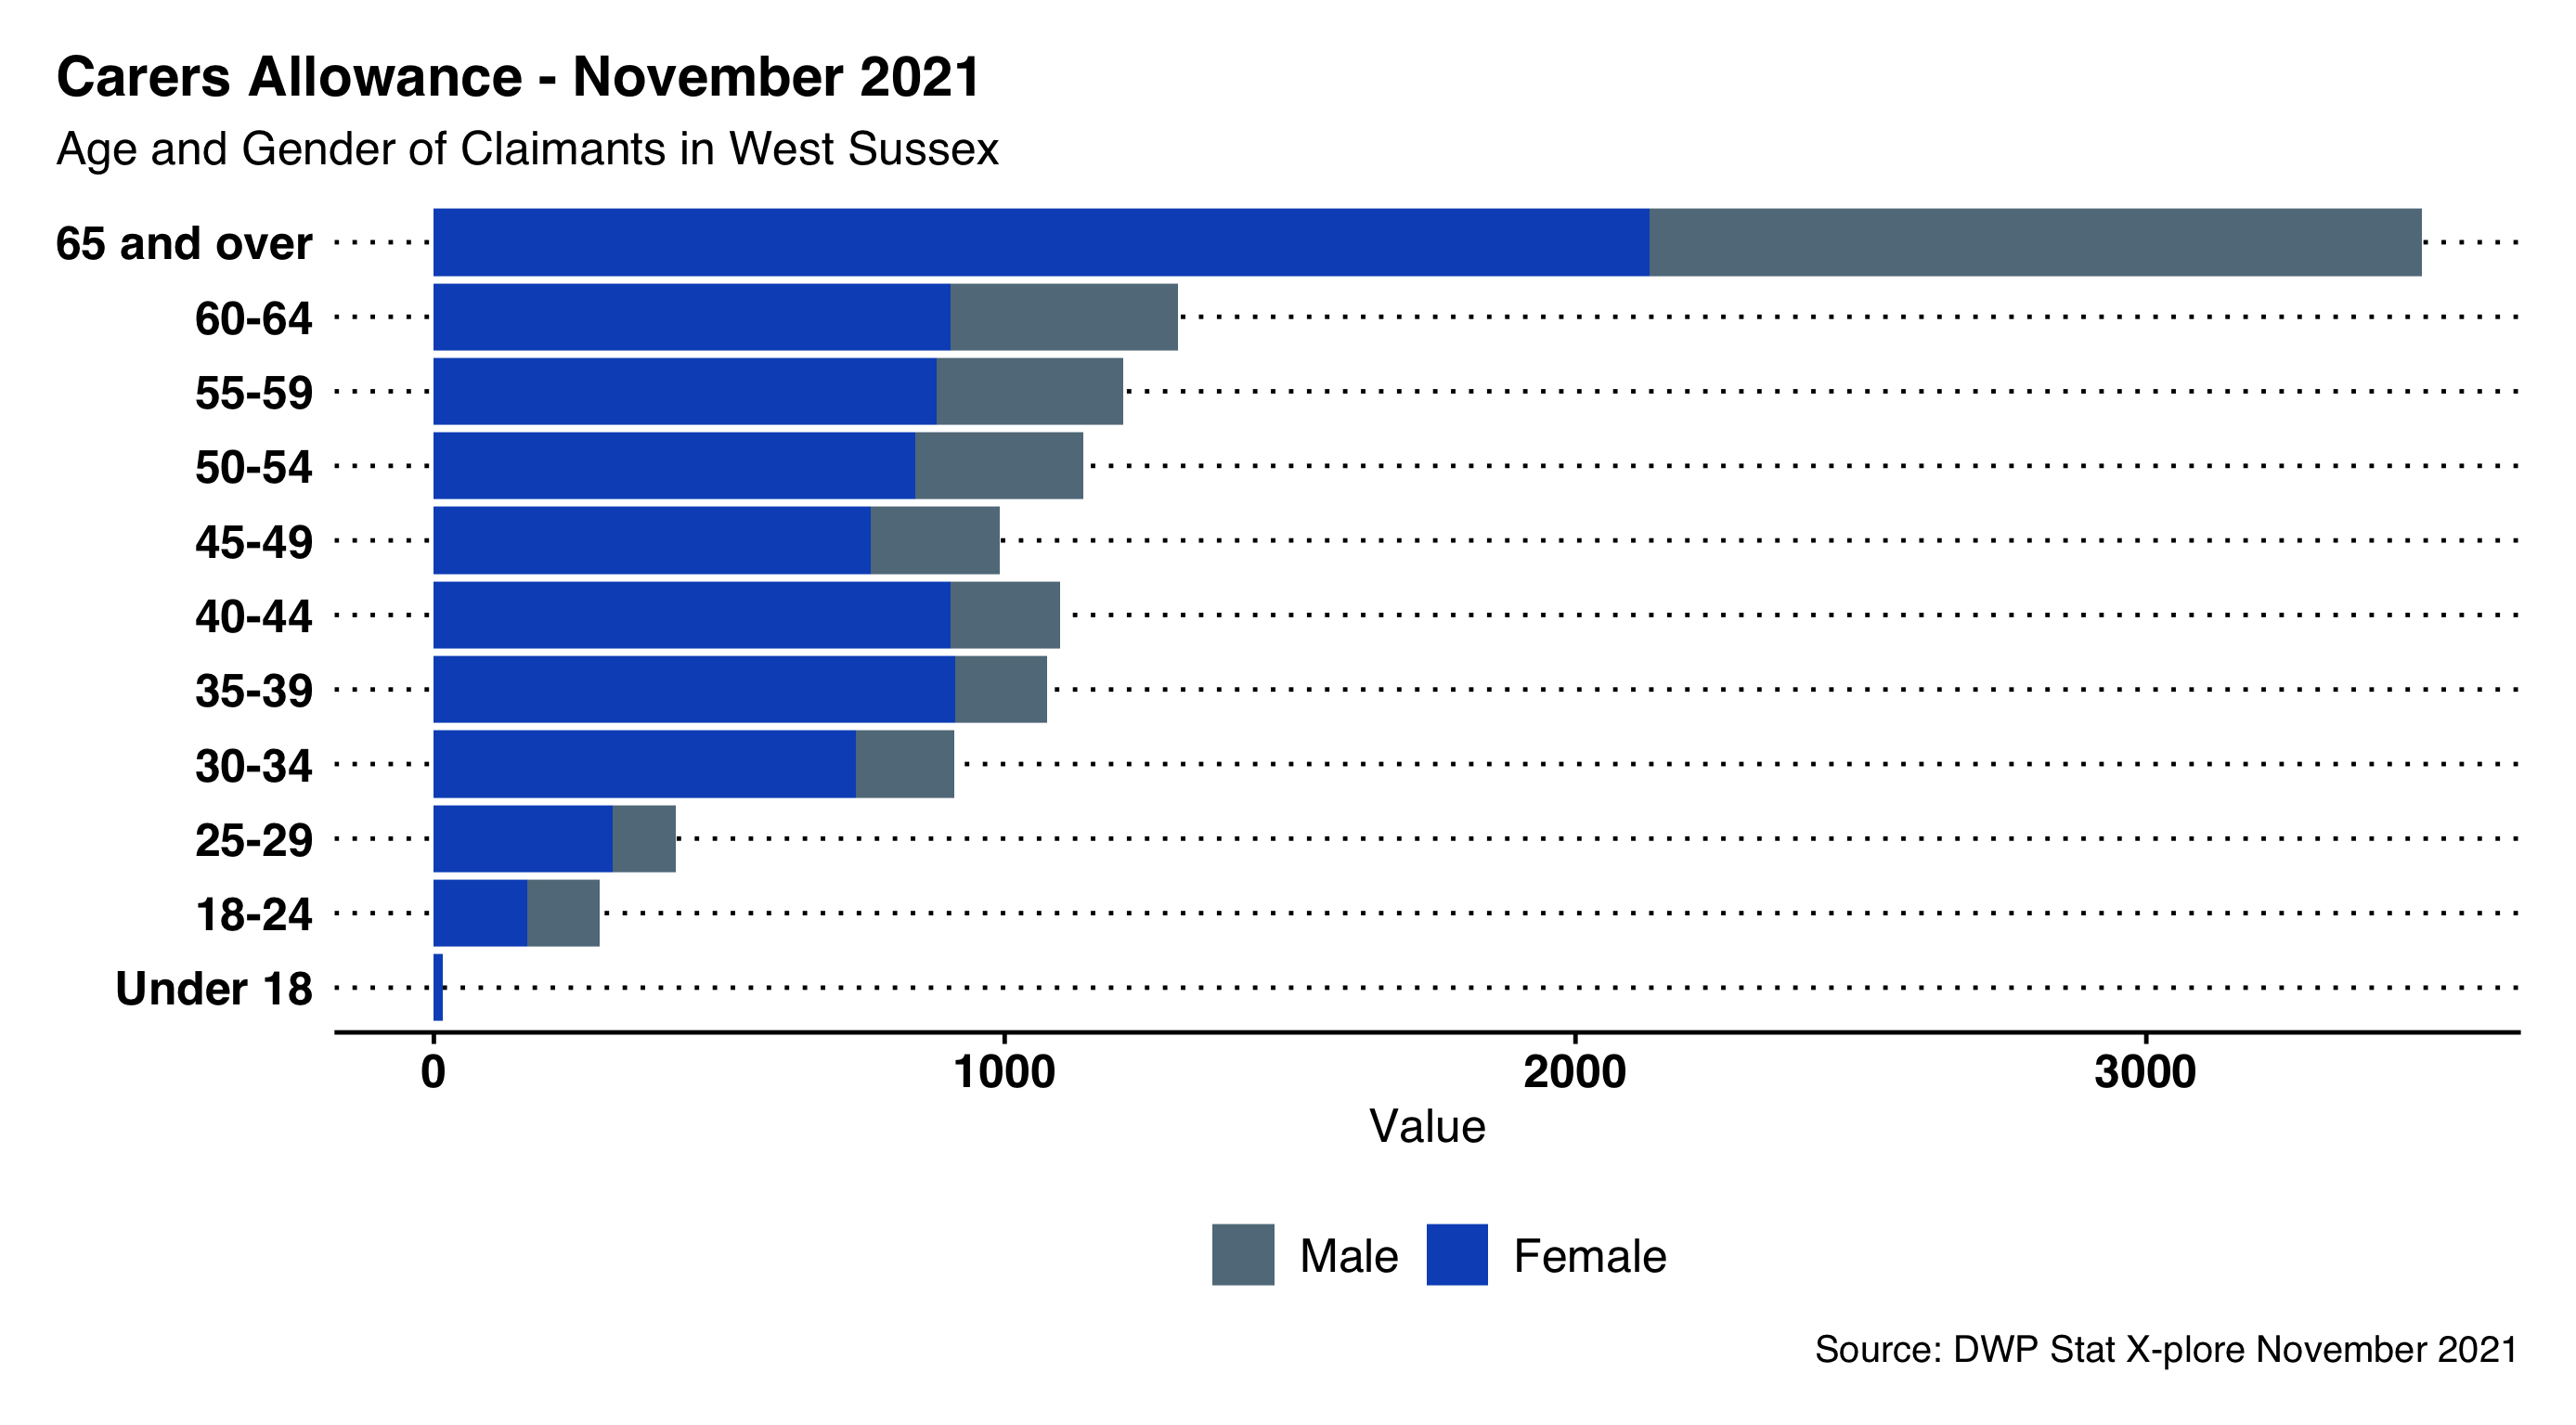
\includegraphics[width=\linewidth]{images/carers_allowance_recipients.png}
\end{figure}


\subsection{Unpaid Care}
\paragraph{Unpaid Care}There are an estimated 90,405 unpaid carers of all ages in West Sussex, representing 10.4\% of the total population (similar to the England proportion).

Women tend to take on more caring responsibilities than men, with an estimated 52,652 female carers compared to 37,704 male carers.

\begin{figure}[h]
    \caption{Estimated number of unpaid carers in West Sussex, by age and sex.}\label{fig:unpaid-carers-sex-age}
    \centering
    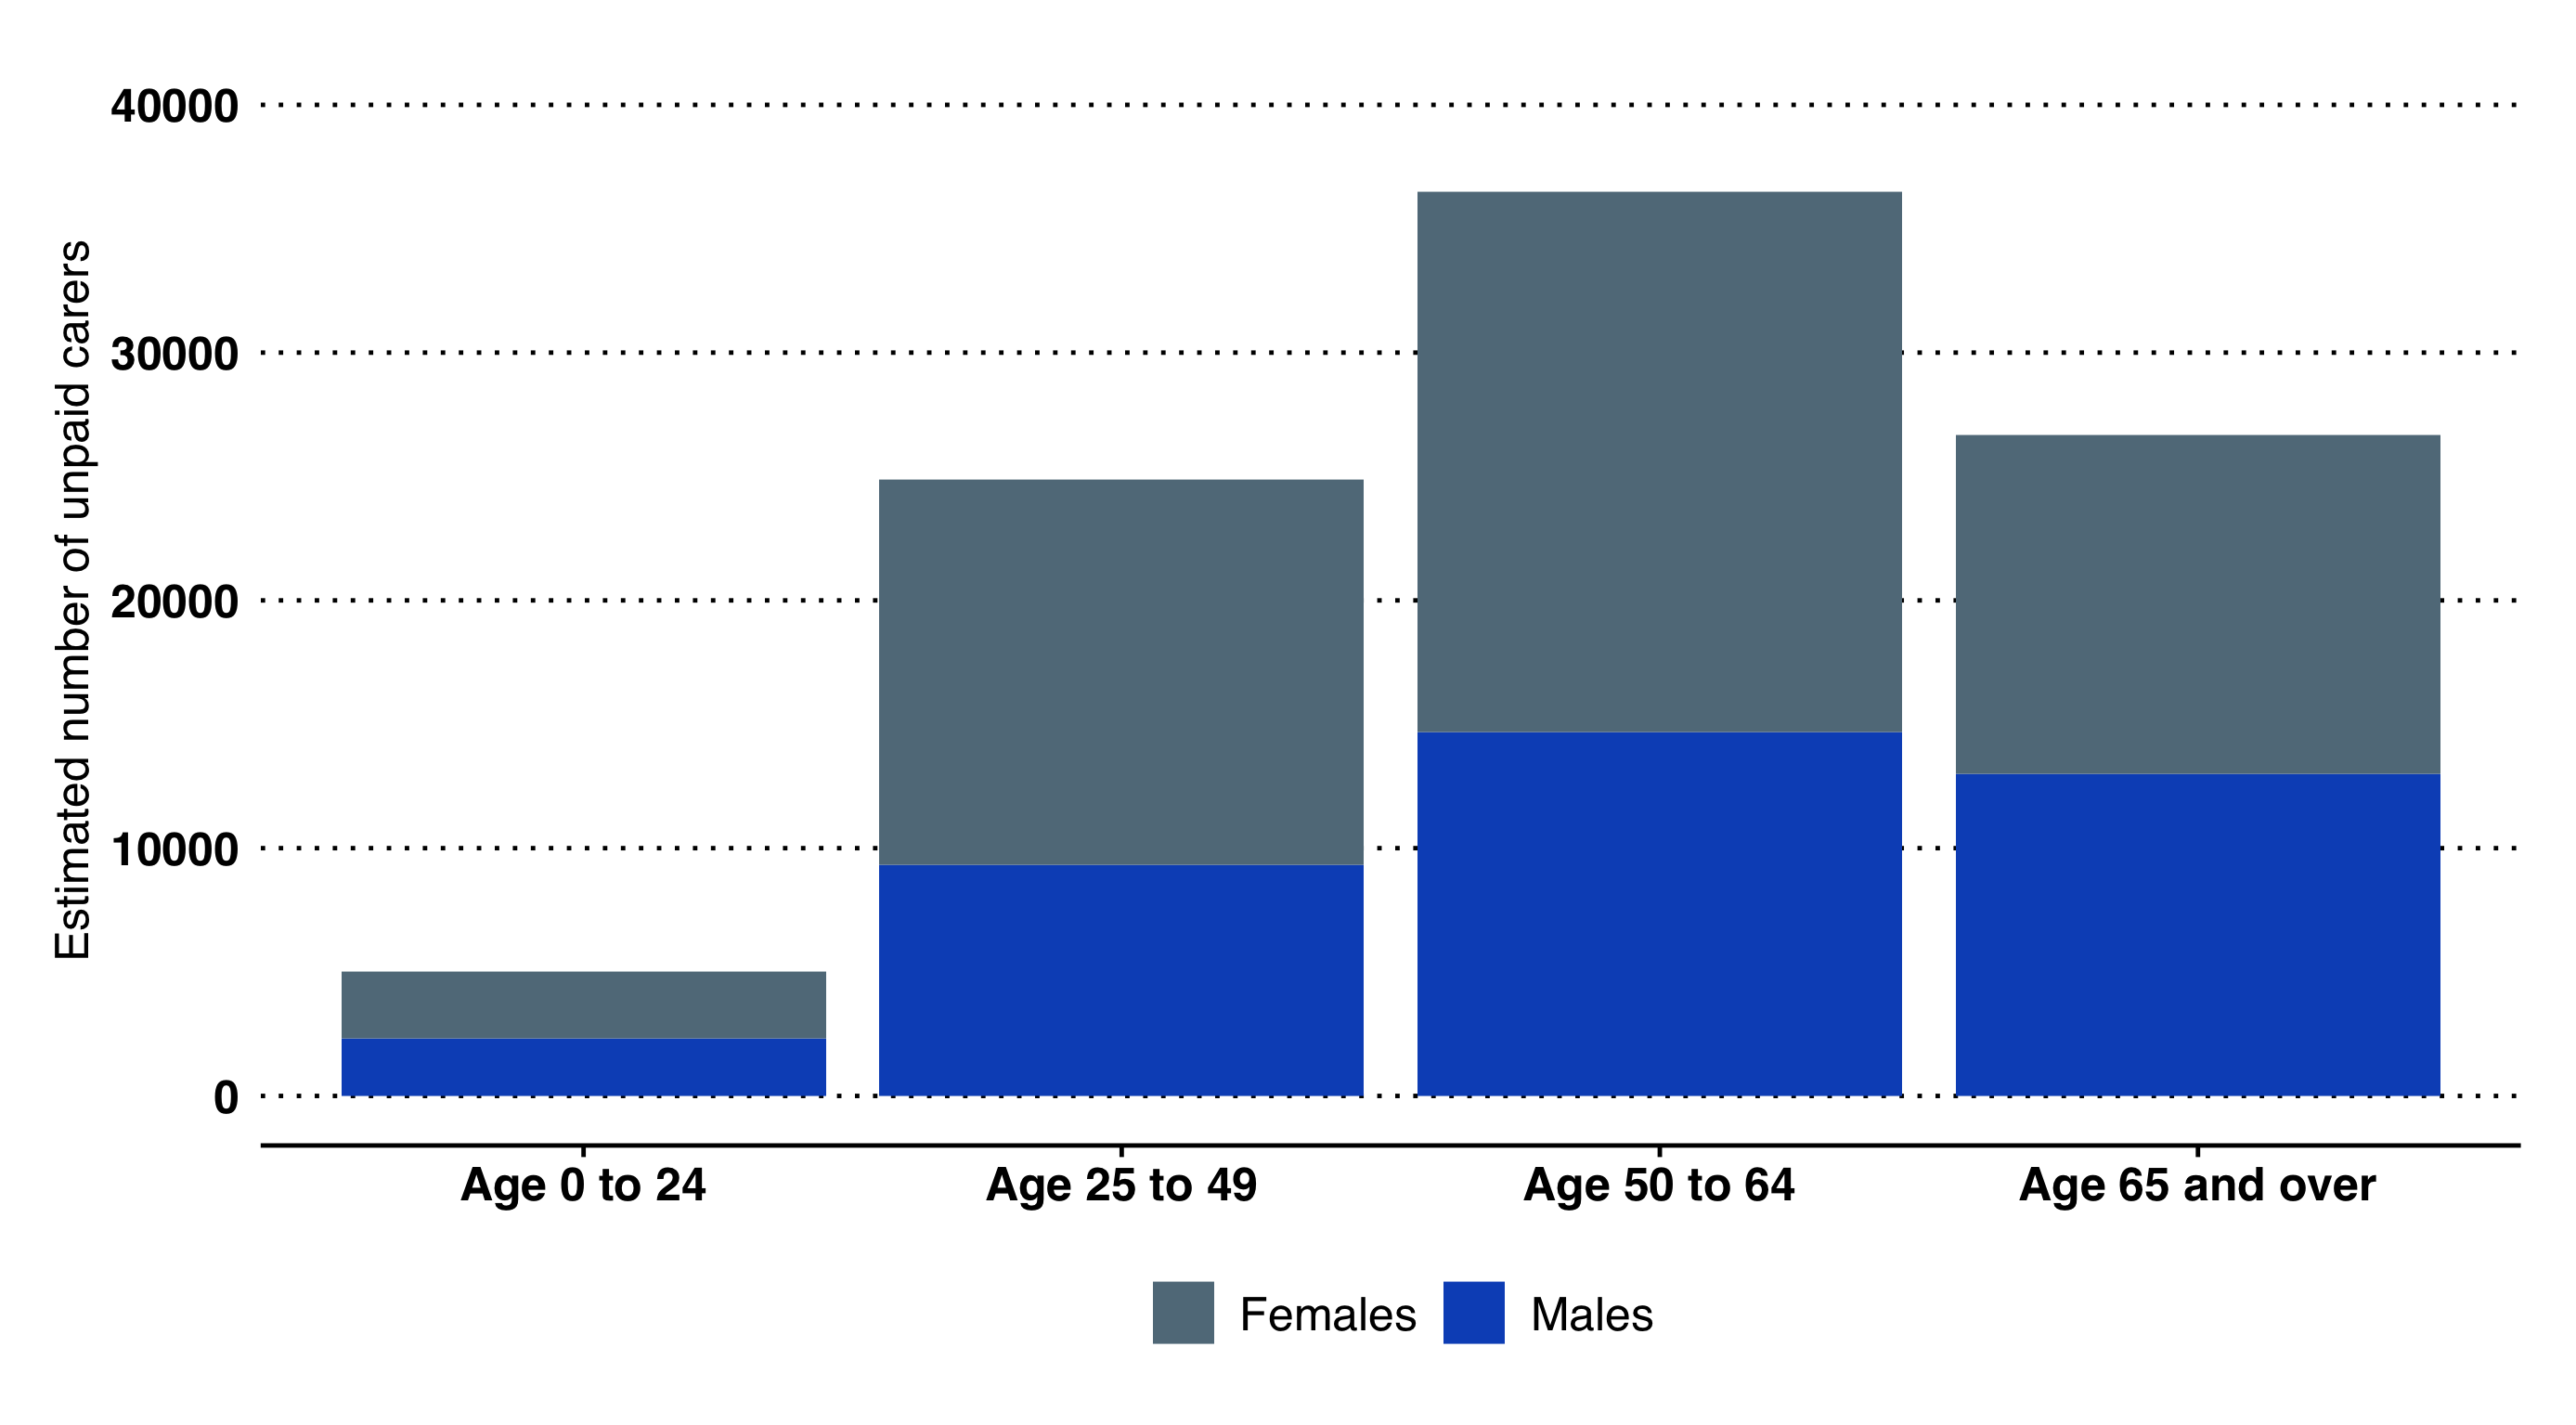
\includegraphics[width=\linewidth]{images/wsx_unpaid_carers_by_age.png}
\end{figure}

Those of working age (ages 25-64) account for 68\% of unpaid care, whilst over- 65s account for 29\%.

Arun has the greatest number of unpaid carers of all ages, at 17,753, followed by Mid Sussex (15,144) and Mid-Sussex (15,042). Adur has the fewest number of unpaid carers, at 7,277.

\paragraph{50 or more unpaid care hours per week}Of the total number of carers in West Sussex, approximately a fifth are estimated to do 50 or more hours of unpaid care a week (slightly below the England proportion). This burden of care again falls more heavily on female carers (over 11,000 female carers, compared to nearly 7,500 male carers, do >50 hours per week).

Over 65s make up the majority of carers doing >50 hours per week; 37.5\% of female carers and 51.6\% of male carers doing >50 hours are in this age-group.

Adur has the greatest proportion of unpaid carers doing >50 hours per week, followed by Arun.

\paragraph{How do we estimate the numbers of unpaid carers?} The Carers Trust defines a carer as anyone who cares, unpaid, for a friend or family member who due to illness, disability, mental health problems or an addiction cannot cope without their support. The current number of unpaid carers in West Sussex can be estimated by applying the percentage of unpaid carers in the population, as recorded in the most recent census (2011), to the latest population estimates (2020).

\newpage

\begin{figure}[H]
    \caption{Estimated number of unpaid carers in West Sussex.}
    \label{figure:unpaidcarers:dabs}
    \centering
    \begin{subfigure}[b]{0.99\linewidth}
        \centering
        \caption{Female carers by West Sussex Local Authorities.}\label{fig:unpaidcarers:dabs:female}
        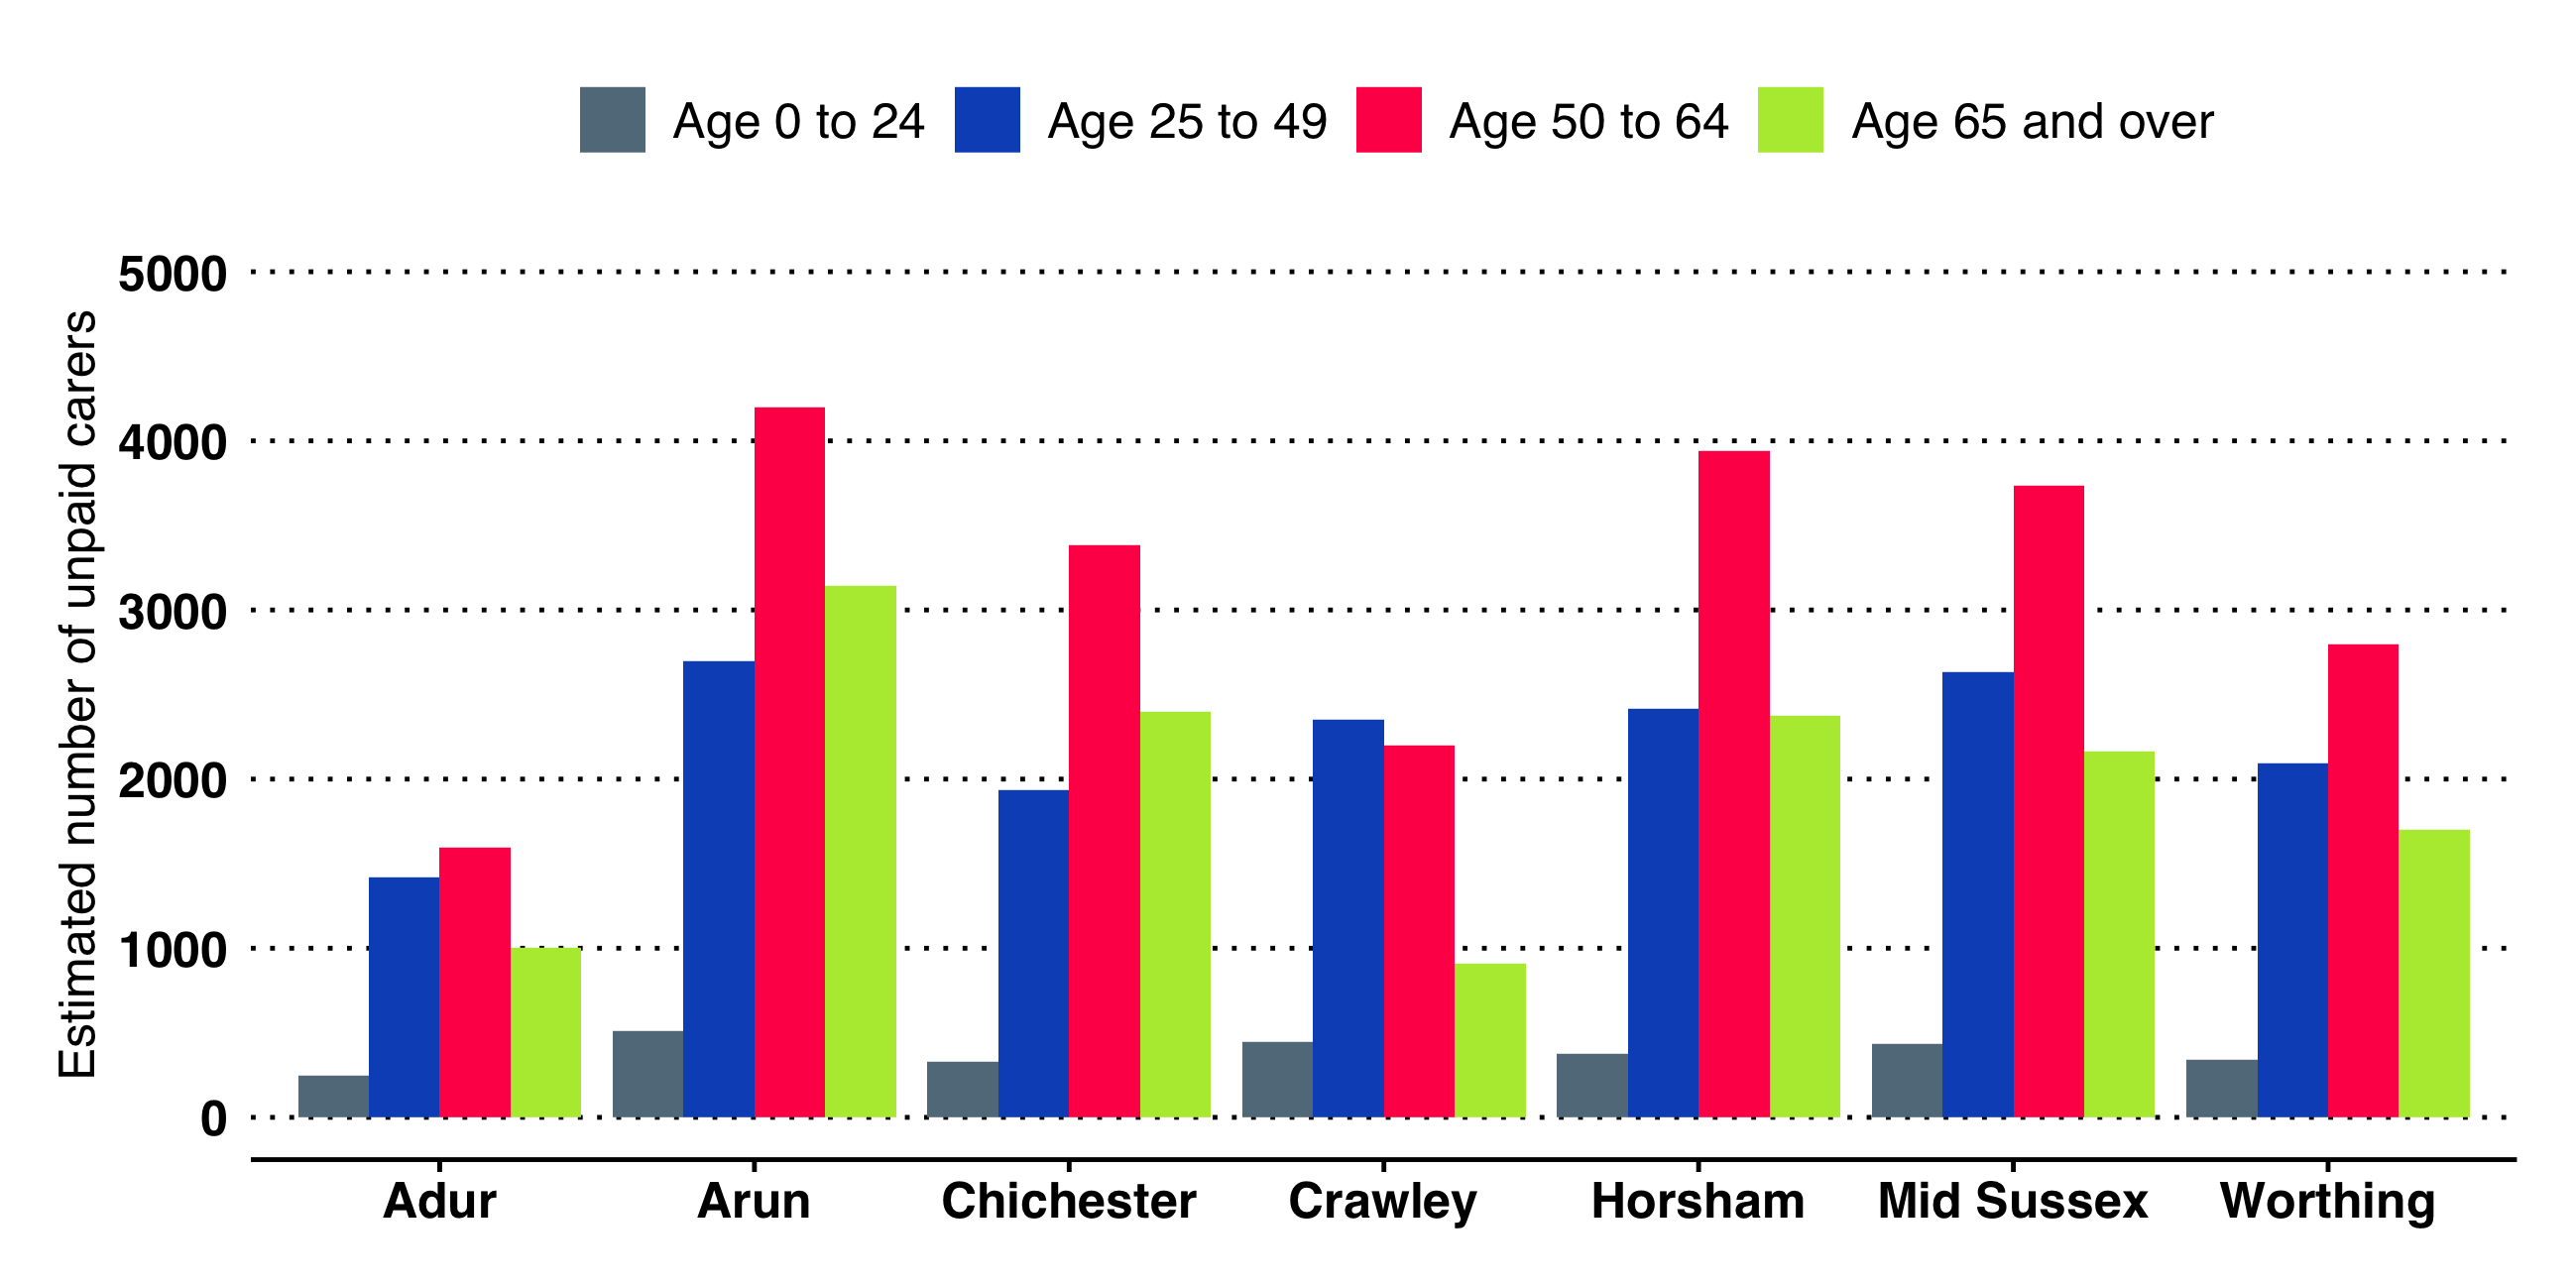
\includegraphics[width=\linewidth]{images/female_unpaid_carers.png}
    \end{subfigure}
    \begin{subfigure}[b]{0.99\linewidth}
        \centering
        \caption{Male carers by West Sussex Local Authorities.}\label{fig:unpaidcarers:dabs:male}        
        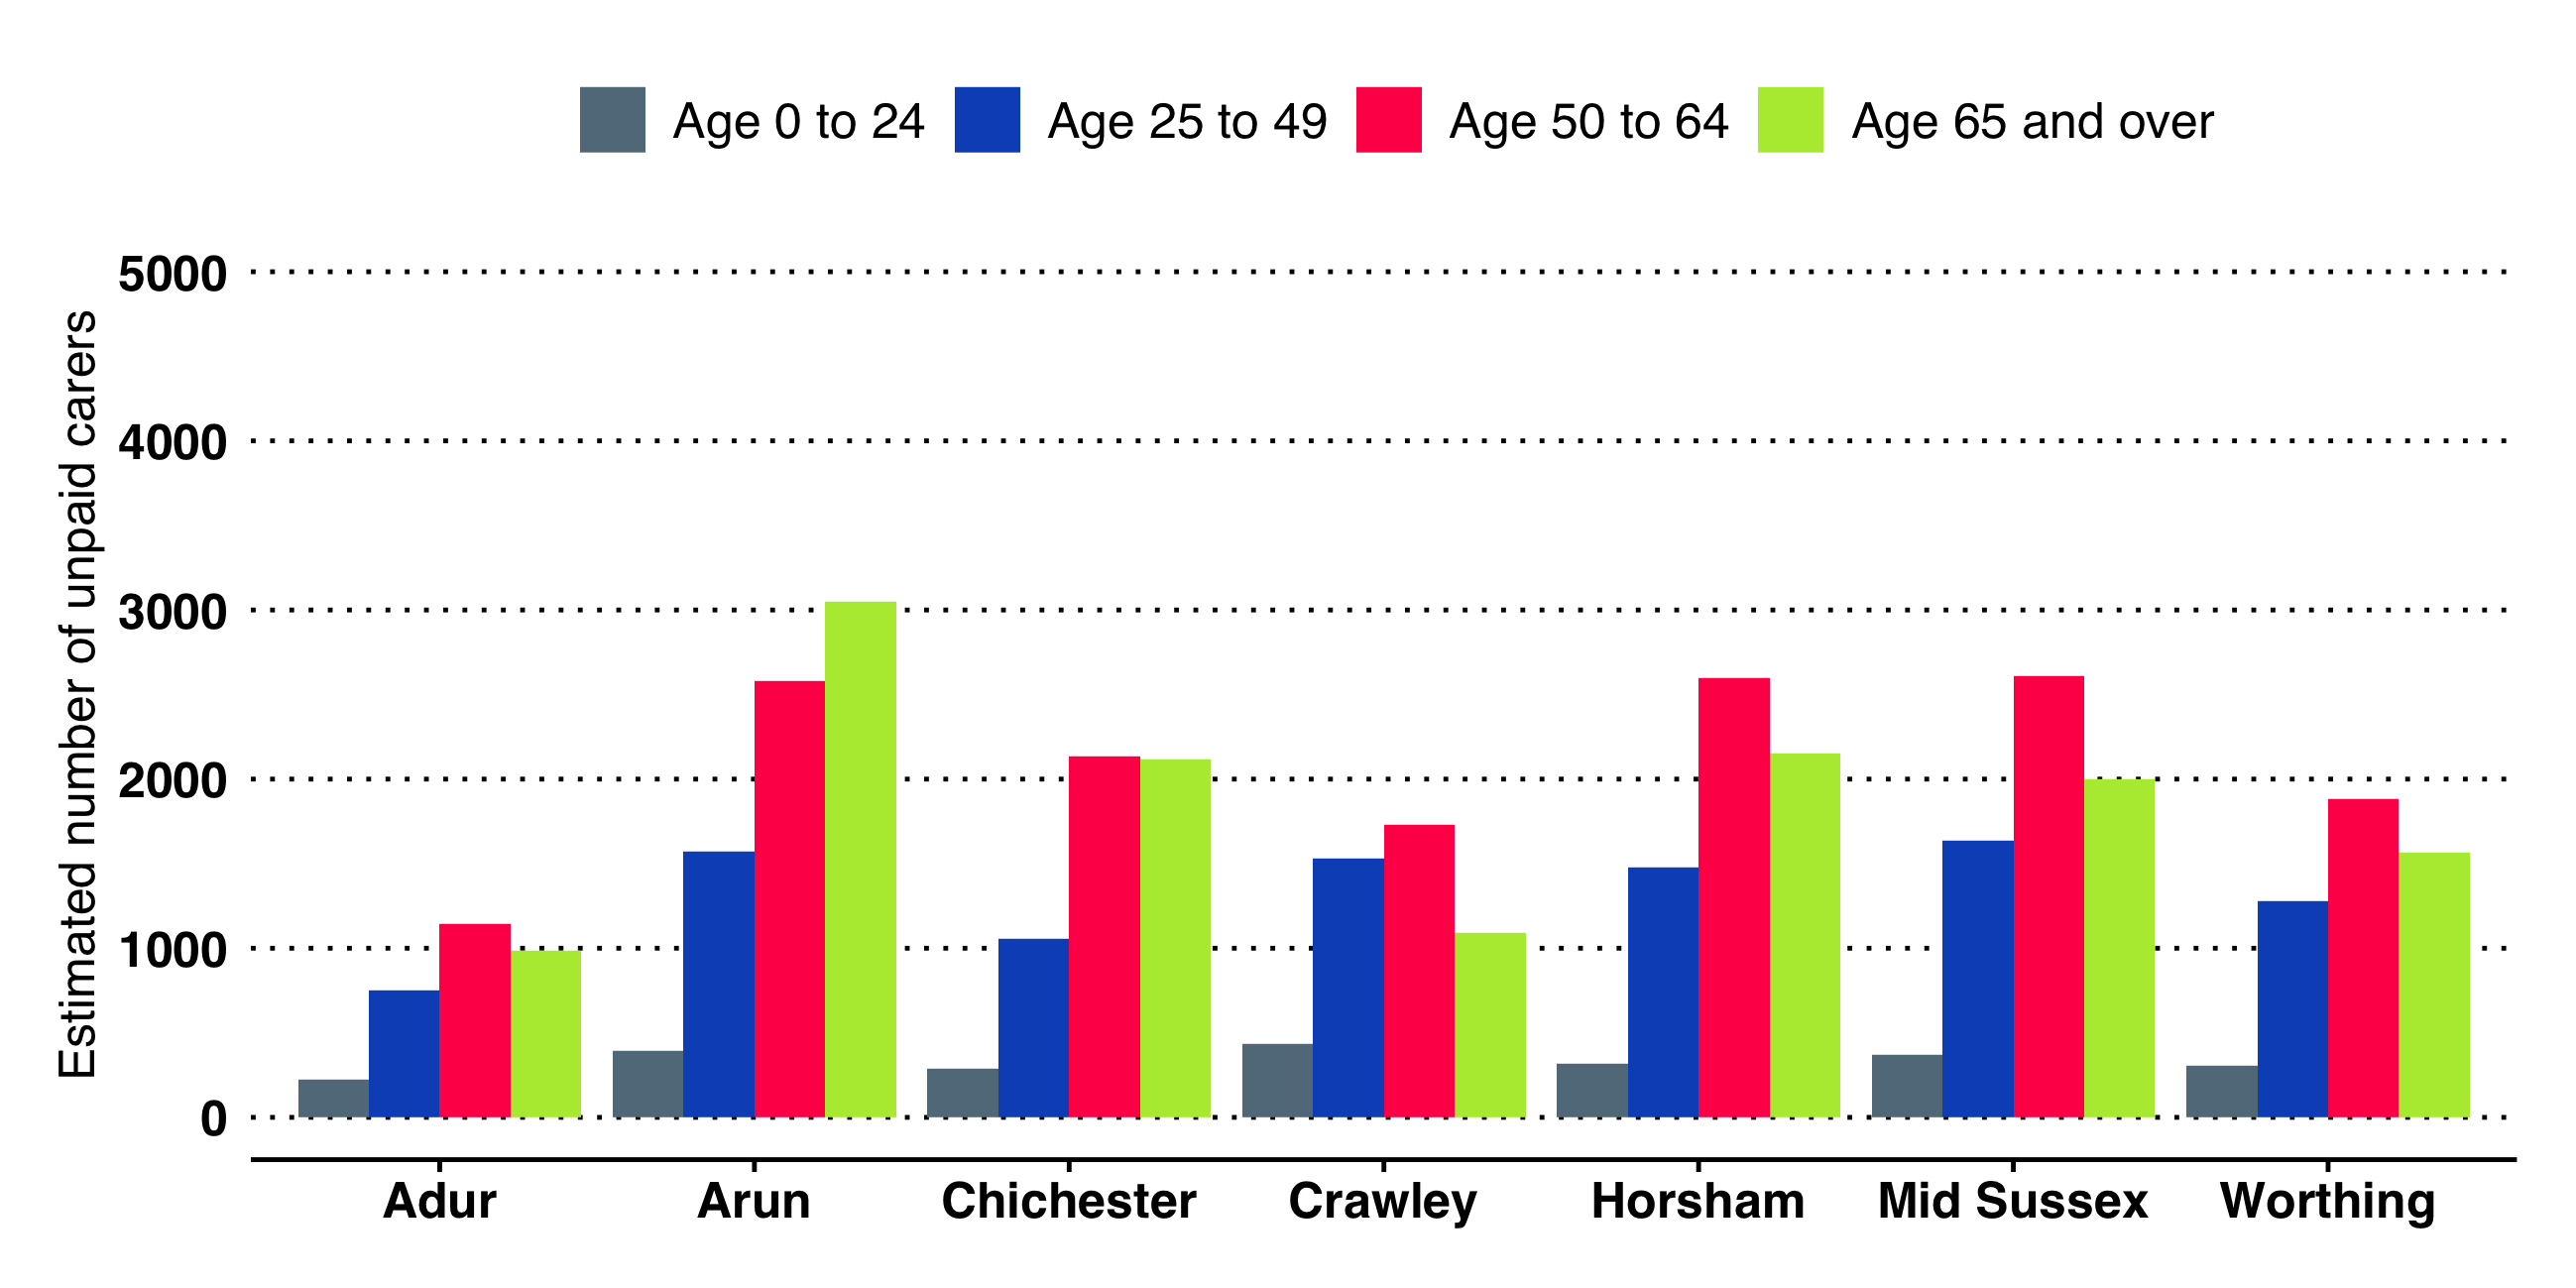
\includegraphics[width=\linewidth]{images/male_unpaid_carers.png}
    \end{subfigure}
    \vspace*{3mm}
\end{figure}

% \paragraph{Carers in the GP Patient Survey} Results from the GP Patient Survey 2019 are shown at West Sussex Clinical Commissioning Group and West Sussex level and compare the experiences of carers and non-carers. Note: these data relate to people registered with a GP Practice who responded to the survey. 

% \begin{itemize}[noitemsep]
%     \item As a proportion of patients, West Sussex has significantly more carers compared to England (18\% vs. 16.9\% of patients), particularly in the Coastal West Sussex CCG (19.3\%).
%     \item The highest proportion of carers was amongst the middle-age groups (45-54 and 55-64 years), with roughly one in four patients in these age-groups providing some care. Compared to England, the proportion of carers aged 55-64 years is higher in West Sussex, and the proportion of 16-24 and 25-34 year olds lower.
%     \item In each West Sussex CCG, over half of carers said they provided support for 1 to 9 hours per week, whilst around one in five carers provided 50 or more hours per week, similar to England.
% \end{itemize}
  
% FIGURE Proportion of carers by number of hours of care provided per week

% \paragraph{Working status} Carers were significantly less likely to be in full-time paid employment compared to non-carers (all ages) in all areas except NHS Horsham and Mid Sussex CCG.

% More carers were looking after the family or home or in part-time paid work than non-carers. However, compared to carers in England, carers in West Sussex were significantly less likely to be in full-time education, looking after the family home, permanently sick or disabled, or unemployed.

% \paragraph{Long-term conditions} Significantly more carers report having a long-term condition (LTC), disability or illness in West Sussex, at 62.5\% of carers compared to around 50\% of non-carers. This proportion is significantly higher, at 65.1\%, in the Coastal West Sussex CCG.

% In West Sussex and England, more carers reported musculoskeletal conditions (arthritis or ongoing problems with back and joints) and long- term mental health issues.

% There was no significant difference in current smoking prevalence between carers and non-carers, and prevalence in West Sussex was significantly lower than England.

% \paragraph{Making Appointments} Fewer carers reported an overall good experience of making an appointment compared to non-carers (63.3\% compared to 69.2\%; similar to England).

% The proportion of patients satisfied with the type of appointment offered was significantly lower amongst carers compared to non-carers, at 71.6\% compared to 76.6\% (similar to England).

% In all areas a except the Crawley CCG, a significantly higher proportion of carers had attempted to access an NHS service when their GP practice was closed, either for themselves or someone else, compared to non-carers.

% A significantly higher proportion of carers had a preferred GP compared to non-carers in all areas (58.1\% Vs. 48.8\%), except the Crawley CCG, although fewer carers reported seeing their preferred GP always or almost always, at 19.1\% VS. 24.3\% of non-carers. This proportion of carers seeing their preferred GP was also significantly lower in West Sussex compared to England (22\%).

\subsection{Health Related Behaviours}
\paragraph{Lifestyle risk factors: smoking; diet; physical activity; and alcohol and other substance misuse.}

West Sussex is relatively healthy with lower levels of "riskier behaviour". However this masks considerable differences between areas, and between groups within the county.

We know that there is a clustering of behaviours; people who smoke are more likely to drink above recommended levels and have lower physical activity rates and so on. This means that there is polarisation taking place, with people who take on key health messages and take steps to lead healthier lives and those who do not. This acts to reinforce and increase existing inequalities.

\paragraph{Smoking}
The following data have been taken from the PHE Local Tobacco Control Profiles. These profiles bring together the range of measures which examine the effects and wider impact of smoking, including prevalence rates, smoking quits and attributable mortality. \url{https://fingertips.phe.org.uk/profile/tobacco-control}

Smoking the remains biggest cause of premature deaths in West Sussex and smoking attributable mortality. There were 3,049 deaths attributed to smoking over the 3 year period between 2017 and 2019.

The overall adult smoking rate in the county has continued to fall. In 2020 the rate was estimated at 11.2\% (CI 8.5\% to 13.9\%)\footnote{PHOF reference C18.} - meaning almost 80,000 people in the county still smoke.

{\bfseries Declines in the smoking rates of people from routine and manual occupations have been smaller.} The most recent survey (2020) estimated the odds of current smoking in West Sussex among routine and manual workers aged 18-64 at 2.0 (CI: 1.2 to 3.4), meaning that prevalence among routine and manual workers could be between 13.4\% and 38.1\%.

In 2020, around a third of people in West Sussex aged 18+ reported being ex-smokers, while 56.4\% reported never having smoked.

\paragraph{Physical Activity and Obesity}
\begin{itemize}[noitemsep]
    \item An estimated 70.2\% of adults were classed as physically active\footnote{PHOF reference C17a. These are adults (aged 19+) who meet CMO recommendations for physical activity (150+ moderate intensity equivalent minutes per week).}. This is higher than England and the average of statistical neighbours. (2020/21 survey data).
    \item 20\% of adults were physically inactive\footnote{PHOF reference C17b. These are adults (aged 19+) that are physically inactive (<30 moderate intensity equivalent minutes per week).}.
    \item The proportion of the adult population meeting the recommended '5-a-day' portions of fruit and vegetables on a 'usual day'\footnote{PHOF reference C15.} in West Sussex was 60.6\%. This is higher than the England rate. Within West Sussex, the majority of districts and boroughs had a rate significantly higher than England, though Arun, Adur, and Crawley are similar to England.
    \item 63.8\% of adults were overweight or obese\footnote{PHOF reference C16.} in West Sussex, similar to comparable authorities and England. In Adur, rates were higher than England whilst the other districts and boroughs were similar to England.
\end{itemize}

\begin{figure}[h]
    \caption{Percentage of overweight or obese adults - West Sussex Local Authorities}\label{fig:obesity:rag}
    \centering
    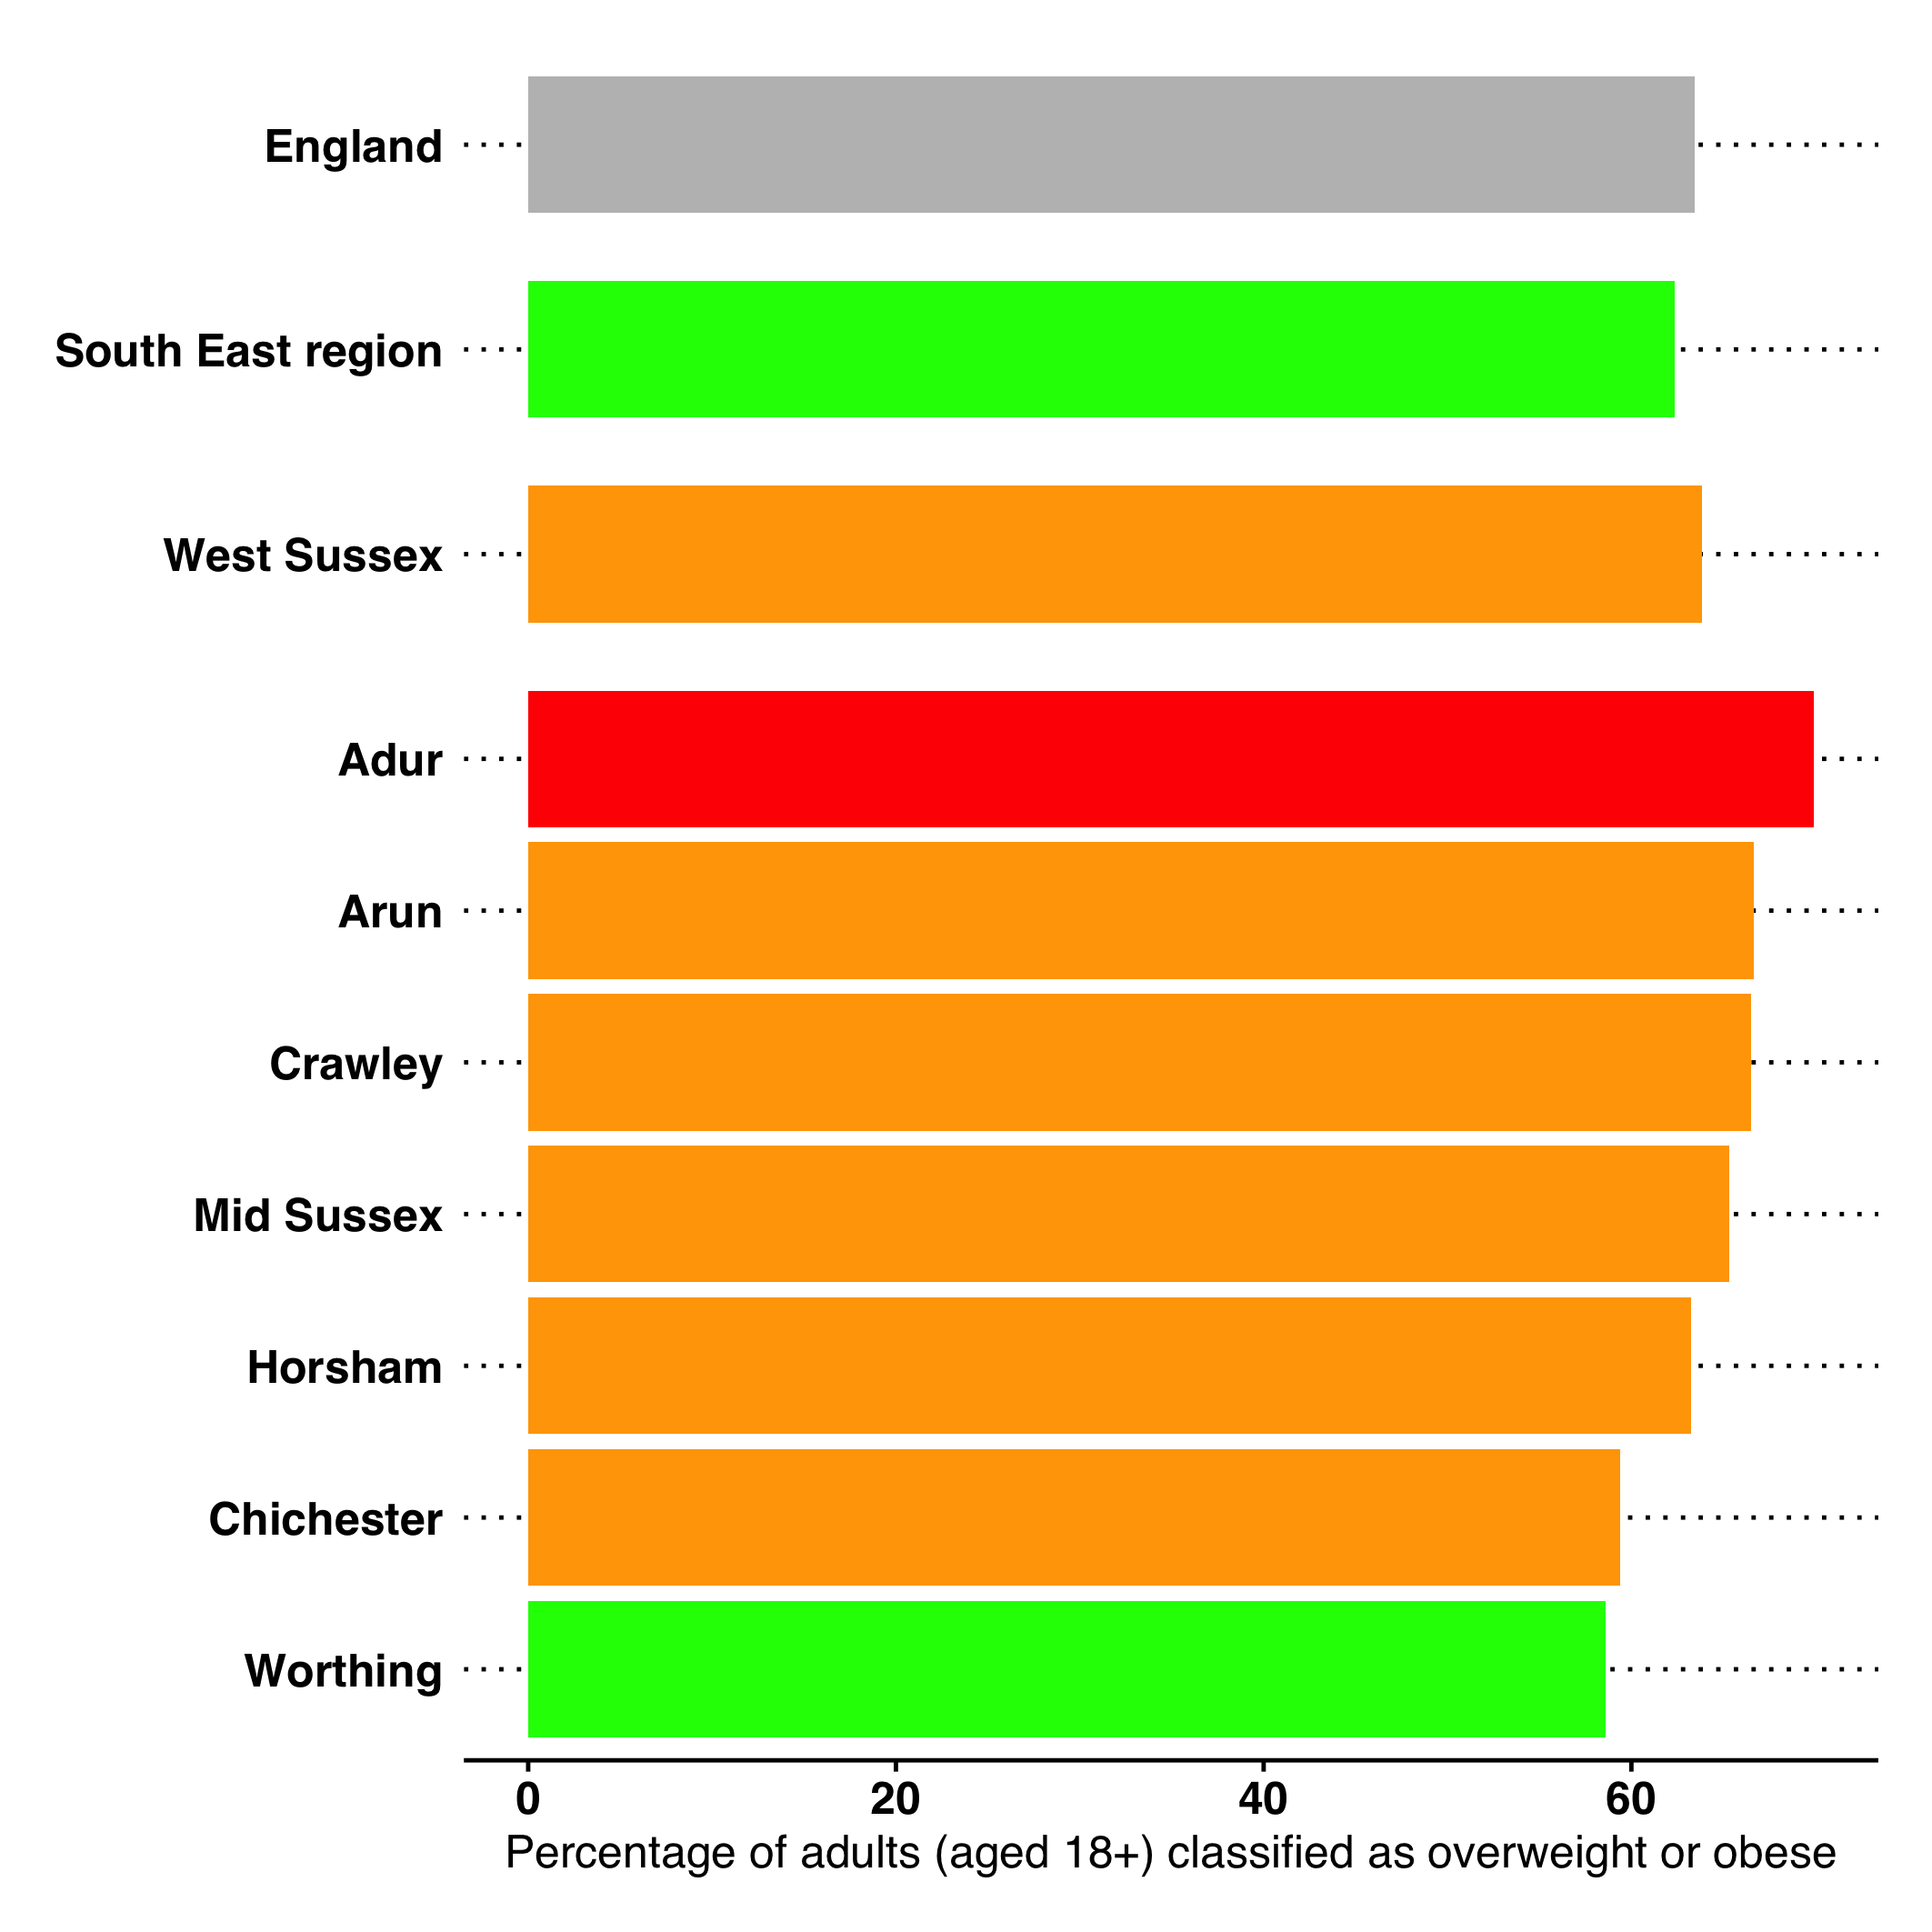
\includegraphics[width=\linewidth]{images/obesity_rag_bar.png}
\end{figure}

\subsection{Substance Misuse}
\subsubsection{Tobacco}
\paragraph{West Sussex Tobacco Control Strategy 2019-2022} Smoking remains the single biggest preventable cause of death and ill health in England. Any differences in smoking prevalence across the population inevitably translate into health inequalities.

The Smokefree West Sussex Partnership is a group of organisations across West Sussex working in partnership to provide strategic direction and leadership on the tobacco control agenda in West Sussex. The West Sussex Tobacco Control Strategy 2019-2022 contributes to realising the Public Health vision for West Sussex and meeting the national objectives through the co-ordinated effort of a wide range of partners. The strategy builds on national plans which establish tobacco control as a comprehensive and coordinated effort to reduce demand, prevent uptake, and support cessation rather than a sole focus on the delivery of smoking cessation services.

The details of the full strategy document and action plan can be found on the JSNA website. An additional website (\url{https://sfws-action-plan.netlify.com/}) provides an interactive version of the strategy to support partners in understanding what actions can be taken, and by who in the short-, medium- and longer- term. 

\subsubsection{Substance Misuse - Alcohol and Drugs} Prevalence Estimates Alcohol-related harm is affected by the amount of alcohol that is consumed and how it is consumed (frequency and intensity of use). Describing patterns of use is therefore complicated. This diagram\footnote{Source: Public Health England, The Public Health Burden of Alcohol and the Effectiveness and Cost-Effectiveness of Alcohol Control Policies An evidence review, 2016} sets out the various terms and estimates (at a national level).

FIGURE - Diagram describing patterns of alcohol use and misuse from PHE

\begin{itemize}[noitemsep]
    \item {\bfseries Abstainers}
    \item {\bfseries Lower Risk Drinking} - drinking less than 14 units per week
    \item {\bfseries Increasing Risk Drinking} - drinking 14 to 50 units a week
    \item {\bfseries Higher Risk Drinking} 50+ units for men a week / 35+ units for women a week
    \item {\bfseries Binge drinking} - drinking of 8+ units (men) / 6+ units (women) on heaviest drinking day in previous week
    \item {\bfseries Dependent Drinkers} - this is derived from data collected as part of the Adult Psychiatric Morbidity Survey (APMS), a national survey of 16+ year-olds. Alcohol dependency is assessed by the Alcohol Use Disorders Identification Test (AUDIT) and the Severity of Alcohol Dependence Questionnaire (SADQ).
\end{itemize}

At {\bfseries West Sussex level} using data from the Health Survey for England (2011 to 2014): 

\begin{itemize}[noitemsep]
    \item 9.6\% of the 18+ population are estimated to be {\bfseries abstainers} - equivalent to 66,600 people in West Sussex (2020 population estimates).
    \item 14.5\% of the 18+ population are estimated to be {\bfseries binge drinkers} - equivalent to 100,700 people in West Sussex.
    \item 23.7\% of the 18+ population are estimated to be {\bfseries drinking 14+ units a week} - equivalent to 168,900 people in West Sussex.
\end{itemize}

Using the APMS, it is estimated that there are 5,500 to 9,300 people in West Sussex with a dependency on alcohol and potentially in need of specialist treatment.

% More up-to-date figures on alcohol misuse needed, especially during and after lockdowns 

\subsubsection{Treatment Outcomes / Impact}
Some of the following data have been taken from the PHE Local Alcohol Profiles for England. These profiles bring together the range of measures which examine the effects and wider impact of alcohol, including alcohol related admissions to hospital, attributable mortality and road accidents. \url{https://fingertips.phe.org.uk/profile/local-alcohol-profiles}

PHE also publish annual estimates of the prevalence of opiate use and/or crack cocaine use. However, data at county level and for specific age groups have not been updated since March 2019. The values presented here are taken from OHID Fingertips.

\paragraph{Alcohol-Related Hospital Admissions} Each rate is for all ages, directly age standardised and measured per 100,000 population. West Sussex compares favourably with England for each rate and is lower than most statistical neighbours. Note that only the specific definition has been updated since 2019.
\begin{itemize}[noitemsep]
    \item There were 583 admissions for alcohol-related conditions (Narrow)\footnote{PHOF reference C21.} per 100,000 (England 664 per 100,000). The number of such admissions in West Sussex was 5,116.
    \item There were 1,887 admissions for alcohol-related conditions (Broad) per 100,000 (England 2,367 per 100,000). The number of such admissions in West Sussex was 17,301.
    \item There were {\bfseries 480 admissions for alcohol-related conditions (Specific) per 100,000} (England 587 per 100,000). The number of such admissions in West Sussex was 4,230.
\end{itemize}
  
\paragraph{Other alcohol-related impacts}
Between 2014 and 2016 there were 206 alcohol-related road traffic accidents in which at least one driver failed a breath test. This represents a rate of 33.8 per 1,000 accidents and is higher than the England rate (26.4) but in line with other comparable local authorities.

\paragraph{Mortality from chronic liver disease} Mortality from chronic liver disease\footnote{PHOF reference E06b}, which is strongly associated with alcohol consumption and obesity, has risen in West Sussex. Recent mortality rates for men and women were significantly lower than the England rate, but this is no longer the case. Using a three year range, the rate is now similar to that of England. Nationally there is evidence that deaths from liver disease are occurring at younger ages.

\begin{figure}[ht]
    \caption{Mortality from chronic liver disease per 100,000 population (All persons, 3 year range)}
    \centering
    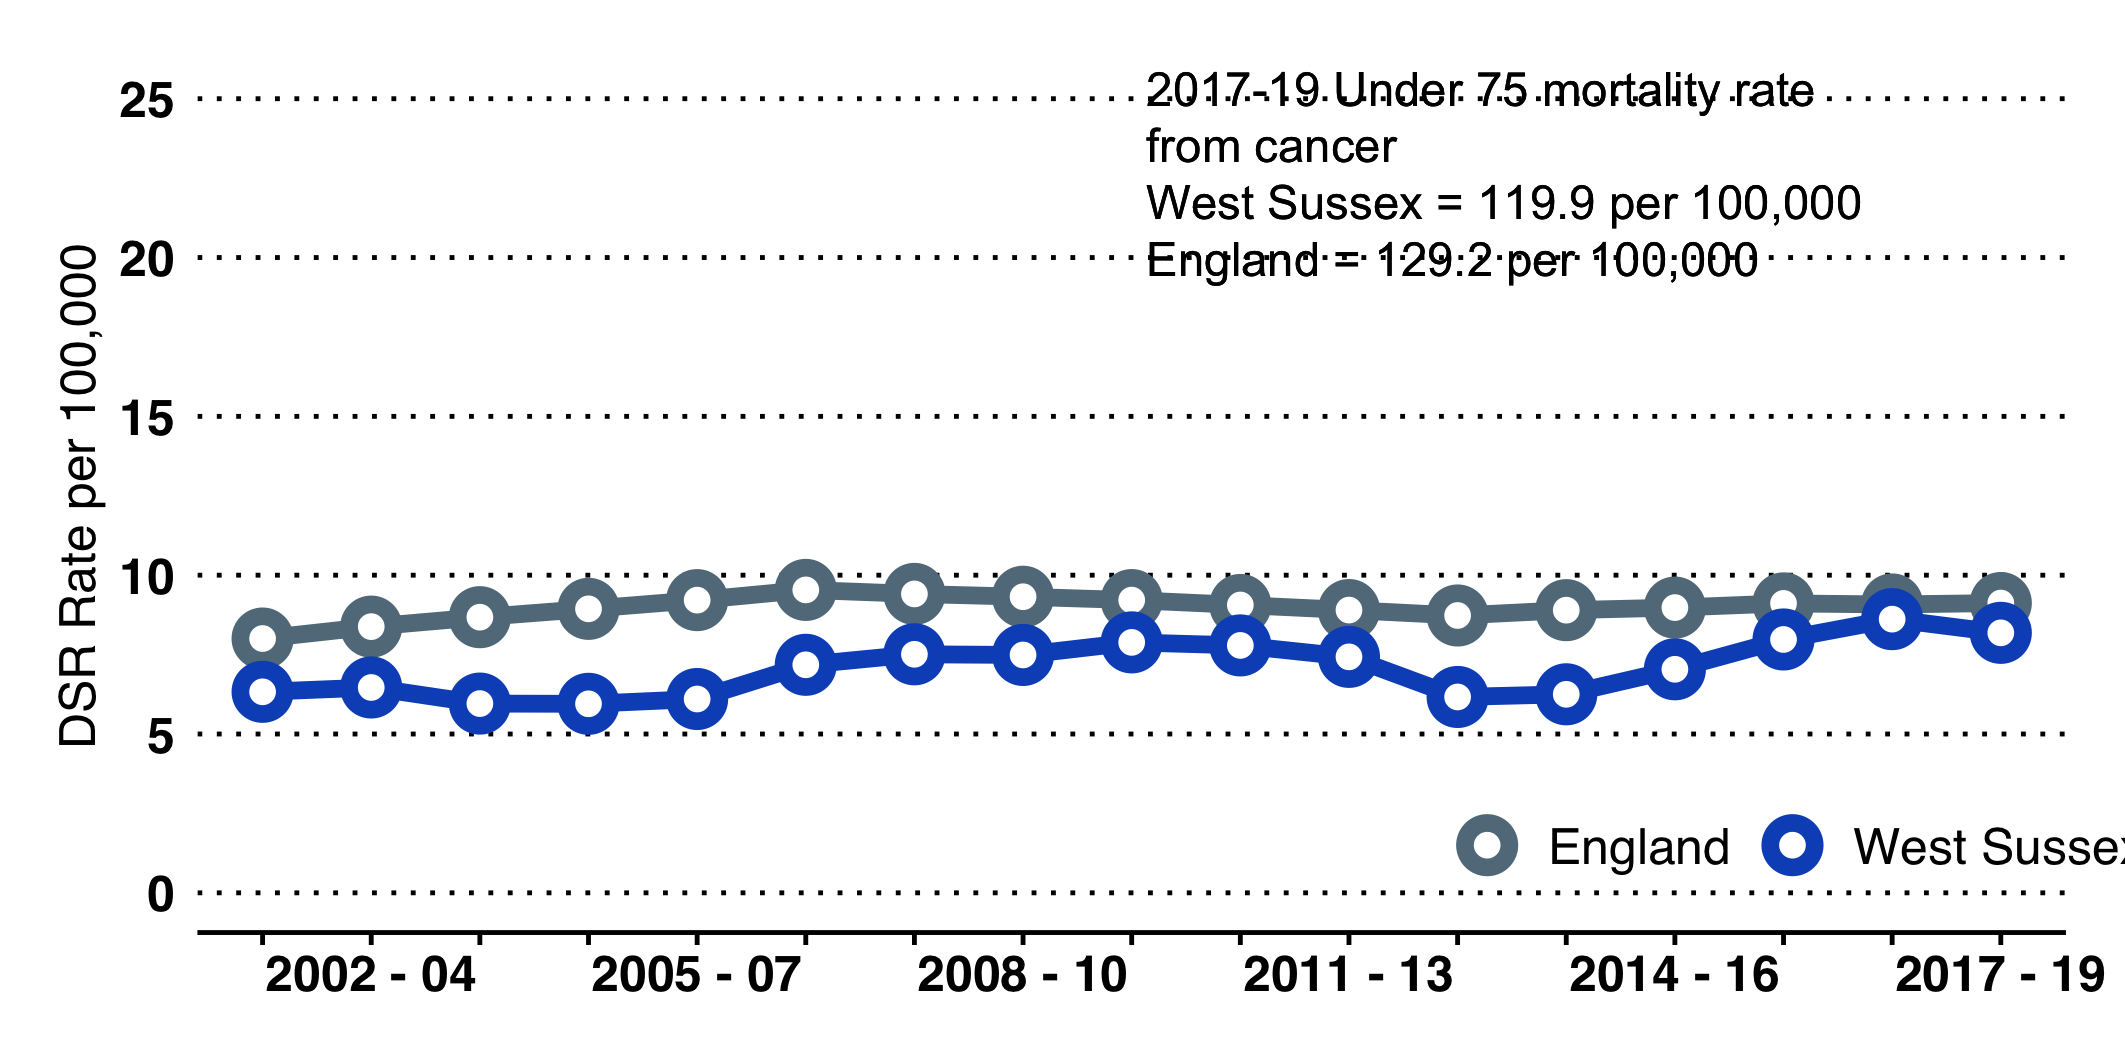
\includegraphics[width=\linewidth]{images/u75_liver_line.png}
    \label{fig:u75_liver}
\end{figure}

\paragraph{Drug misuse} It is estimated that between 1,400 and 4,100 people (aged 16-64 years) use opiates and/or crack in West Sussex, 70\% of which are 35 years or older. In 2018-2020, there were 78 deaths in West Sussex classified as drug misuse deaths\footnote{PHOF reference C19d}. Although the rate of drug related deaths in West Sussex remains lower than the England rate (3.2 per 100,000 compared to 5.0 nationally) a recent upward trend has begun to stabilise.

\paragraph{Treatment Outcomes}
There have been improvements in recent years in the successful completion rates of treatment in West Sussex. Note there is a time lag on these measures and numbers are low - notably for opiate drug users.

\begin{itemize}[noitemsep]
    \item 32.9\% of {\bfseries alcohol users} that left treatment successfully\footnote{PHOF reference C19c} in 2020 did not re-present to treatment within 6 months (England rate 35.3\%). This is similar to other comparable local authorities (33.7\%).
    \item 31.4\% of {\bfseries non-opiate drug users} who left treatment successfully\footnote{PHOF reference C19b} did not re-present to treatment within 6 months (England rate 33.0\%). This has improved in recent years, with the rate similar to England and comparable local authorities (34.5\%).
    \item 5\% of opiate drug users who left treatment successfully\footnote{PHOF reference C19a} did not re-present to treatment within 6 months (England rate 4.6\%). This is similar to the England rate but less than the average of  comparable local authorities (5.7\%, CI: 5.4\%-6.1\%).
\end{itemize}

\paragraph{People NOT in Receipt of Treatment (2018/19)} Using prevalence estimates and data from treatment services (from the National Drug Treatment Management System (NDTMS)), we can estimate the percentage of people with an alcohol dependency and users of opiates and/or crack cocaine (OCU) who are not in receipt of treatment.

\begin{itemize}[noitemsep]
    \item The estimated proportion of the West Sussex OCU users in 2018/19 who were {\bfseries not in contact with drug treatment services for an OCU problem was 51\%} (approximately 1,350 people).
    \item The estimated proportion of the West Sussex dependent drinkers in need of specialist alcohol treatment who were {\bfseries not in contact with treatment services for alcohol only or alcohol and non-opiate use was 78.3\%} (approximately 5,600 people).
\end{itemize}
 
\paragraph{Drug Use} The Royal Society for Public Health report 'Taking a New Line on Drugs' (2016)\footnote{Source: RSPH Taking a New Line in Drugs \url{https://www.rsph.org.uk/our-work/campaigns/taking-a-new-line-on-drugs.html}} sets out the challenge of reducing drug-related harm.

It notes that:

\begin{itemize}[noitemsep]
    \item Many substances that cause harm are legal and socially embedded, including alcohol, tobacco and prescription drugs.
    \item Harm is multi-faceted, including harm to individuals, others and the wider society.
    \item The relationship between drugs and mental health is complex. People may use drugs for a psychological effect and use can result in feelings of anxiousness, depression etc.
    \item Some people are at a higher risk of drug use and harm than others. People with pre-existing mental health conditions, including anxiety and depression, are particularly at risk.
    \item Drug harm can affect all ages and communities, but it is known that harm disproportionately affects people from more deprived communities.
\end{itemize}

%\subsection{A Focus on Drug Related Deaths}
%\paragraph{Background} In 2016, Public Health England released a report into the sharp rise of Drug Related Deaths (DRDs) seen between 2013 and 2015, which reached the highest national levels yet seen in 2015\footnote{PHE (2016). Understanding and preventing drug-related deaths: The report of a national expert working group to investigate drug-related deaths in England}. This included a 21\% increase in 2013 and a 17\% increase in 2014. ONS figures also indicated a 64\% increase in heroin-related death registrations from 2013 to 2015. The subsequent 2017 West Sussex Suicide Audit, which examined deaths between 2013 and 2015, revealed 42 individuals had taken their own lives by self -poisoning (20\% of all suicides in the three-year period).

%\paragraph{West Sussex Drug Related Deaths} The newly designed West Sussex Drug Related Deaths Audit covered the period between 1st January 2015 to 31 st December 2017 and reviewed 123 deaths. Although Public Health teams and Commissioning managers collect data on those who have died whilst connected to community services, which are essential to preventing early death, this alone does not provide insight into the wider population or the individuals identified in this audit who were not involved with services at any point. Examining the barriers and facilitators to service engagement can help in refocusing efforts to engage with more residents.

%The full report of the audit is available on the JSNA website. Contact Robert Whitehead (\url{robert.whitehead@westsussex.gov.uk}) for more information.

%\subsubsection{Key points}
%\begin{itemize}[noitemsep]
%    \item There were 123 deaths from drug poisonings in the three-year period the audit examined. Over a quarter of these were suicides and more than half were accidental overdoses. Roughly half of all deaths were classed as drug misuse.
%    \item Males accounted for two thirds of all deaths. Half of these involved controlled substances and males accounted for 86\% of all drug misuse deaths, particularly focused between ages of 25 and 44 years.
%    \item Female deaths were spread more evenly among older age groups and were explained by a higher proportion of accidental overdoses and suicides involving prescribed medications. Drug misuse was ascribed to 24\% of female deaths.
%    \item Eight males had been in prison or involved with probation services in the past year (9\% of male deaths).
%    \item Ten males were known to be homeless or of no fixed abode (16\% of all drug misuse deaths).
%    \item Four in every five deaths occurred in the home or the home of another. Only 9\% of deaths occurred in a public area.
%    \item There was an increase in overdoses on Saturdays and suicides on Sundays.
%    \item Evidence around Naloxone intervention and resuscitation attempts were not sufficiently documented to report on in this audit.
%\end{itemize}

\subsection{Sexual Health}
%To inform the re-procurement of local sexual health services, a detailed needs assessment was undertaken in 2019. This is available on the JSNA website. On the next few pages are a selected number of metrics from the needs assessment, many of which are from the Public Health Outcomes Framework. The latest published data are available in the local Sexual and Reproductive Health Profile on PHE Fingertips.

%For further information contact Dr Matthew Dorey (\url{matthew.dorey@westsussex.gov.uk}).

\paragraph{Key Points} In 2018, there were a total of 2,984 new STI diagnoses (all STIs), a rate of 344 per 100,000 population. This is a large decrease compared to 2019, which had the highest rate of new diagnoses in West Sussex in the previous 5 years, and below the national rate (562 per 100,000) along with comparable local authorities. While local services did provide an online service supplying self-testing kits, it is likely that the number of diagnoses is a result of Covid-19. 

\begin{table}
    \caption{Number and rate of specific STI diagnoses in West Sussex, 2020.}
    \centering
    \begin{tabular}{llll}
    \toprule
    STI & Number of diagnoses & Rate (West Sussex) & Rate (England) \\
    \midrule
    Chlamydia & 1336 & 154 & 286 \\
    Genital warts & 455 & 52.4 & 48.6 \\
    Genital herpes & 330 & 38 & 36 \\
    Gonorrhoea & 351 & 40 & 101 \\
    Syphilis & 84 & 9.7 & 12.2 \\
    \bottomrule
    \end{tabular}
    \label{tab:wa:stis}
\end{table}

Rates of new STI diagnoses for Chlamydia, Gonorrhea, Syphilis, Genital Herpes and Genital Warts are consistently below the England rate. However, the rates of the former three have been increasing over the past ten years, at a similar rate of increase to England. Compared to similar authorities, diagnosis rates for Gonorrhea, Herpes and Syphilis in West Sussex are amongst the highest.

The overall testing rate (excluding for Chlamydia in under 25s), a metric strongly associated with the level of diagnoses, was 3583.7 per 100,000 in 2020, remaining significantly lower than the England rate (4549.3 per 100,000) and 9th highest amongst CIPFA neighbours.

The proportion of late HIV diagnoses (i.e. where the CD4 cell count is less than 350 per mm3 )\footnote{PHOF reference D07. Late diagnosis is the most important predictor of morbidity and mortality among those with HIV infection.} has increased in recent years, to approximately 52\% in 2018 - 2020. This is higher than England (42.4\%) and equates to 50 late HIV diagnoses in West Sussex between 2018 - 2020.

%Overall attendances at sexual health venues increased from 24,300 to 28,900 between 2013 and 2017. The proportion of people receiving a sexual health screen on first attendance increased from 68\% to 79\% over the same time period.

In 2020, there were 148 conceptions in under-18 year-olds\footnote{PHOF reference C02a.}, a slight decrease on 2019. The rate of 11.1 per 1,000 15-17 year-olds is similar to England. 63\% of teenage conceptions ended in abortion in West Sussex (England, 53\%).

In 2020, the rate of abortions per 1,000 females aged 15-44 in West Sussex was 17.1, in line with comparable authorities and below the England rate (18.9/1,000), although higher than the previous 8 years. The percentage of abortions undertaken under 10 weeks in West Sussex is, at 88.7\%, similar to England (88.1\%) and 7th lowest amongst comparable authorities. Of the abortions to women aged under 25 years, 25.3\% (212 abortions) were repeat abortions i.e. to women who had had previous abortions.

The use of long acting reversible contraception\footnote{PHOF reference C01. This measure excludes LARC injections.} in West Sussex is relatively high (51.6 per 1,000 female population aged 15-44 years in 2020) compared with similar authorities and England (34.6/1,000). All rates are considerably lower than 2019, highlighting the difficulty of accessing these services during the Covid-19 pandemic.

The hospital admission rate for Pelvic Inflammatory Disease (PID) in West Sussex has been high in recent years. Between 2016/17 and 2019/20, admissions rates were significantly higher than the England rate. In 2019/20 the rate in West Sussex the rate was 329.9 per 100,000 compared to 254.7 per 100,000 in England. Rates fell significantly in both West Sussex and England during 2020/21, with the rate for West Sussex 191.6 per 100,000 higher than that for England (186.2 per 100,000).
 
\begin{figure}[ht]
    \caption{Teenage conceptions have steadily declined in the last 20 years, although two of the past three years have seen small increases.}\label{fig:teen_conc}
    \centering
    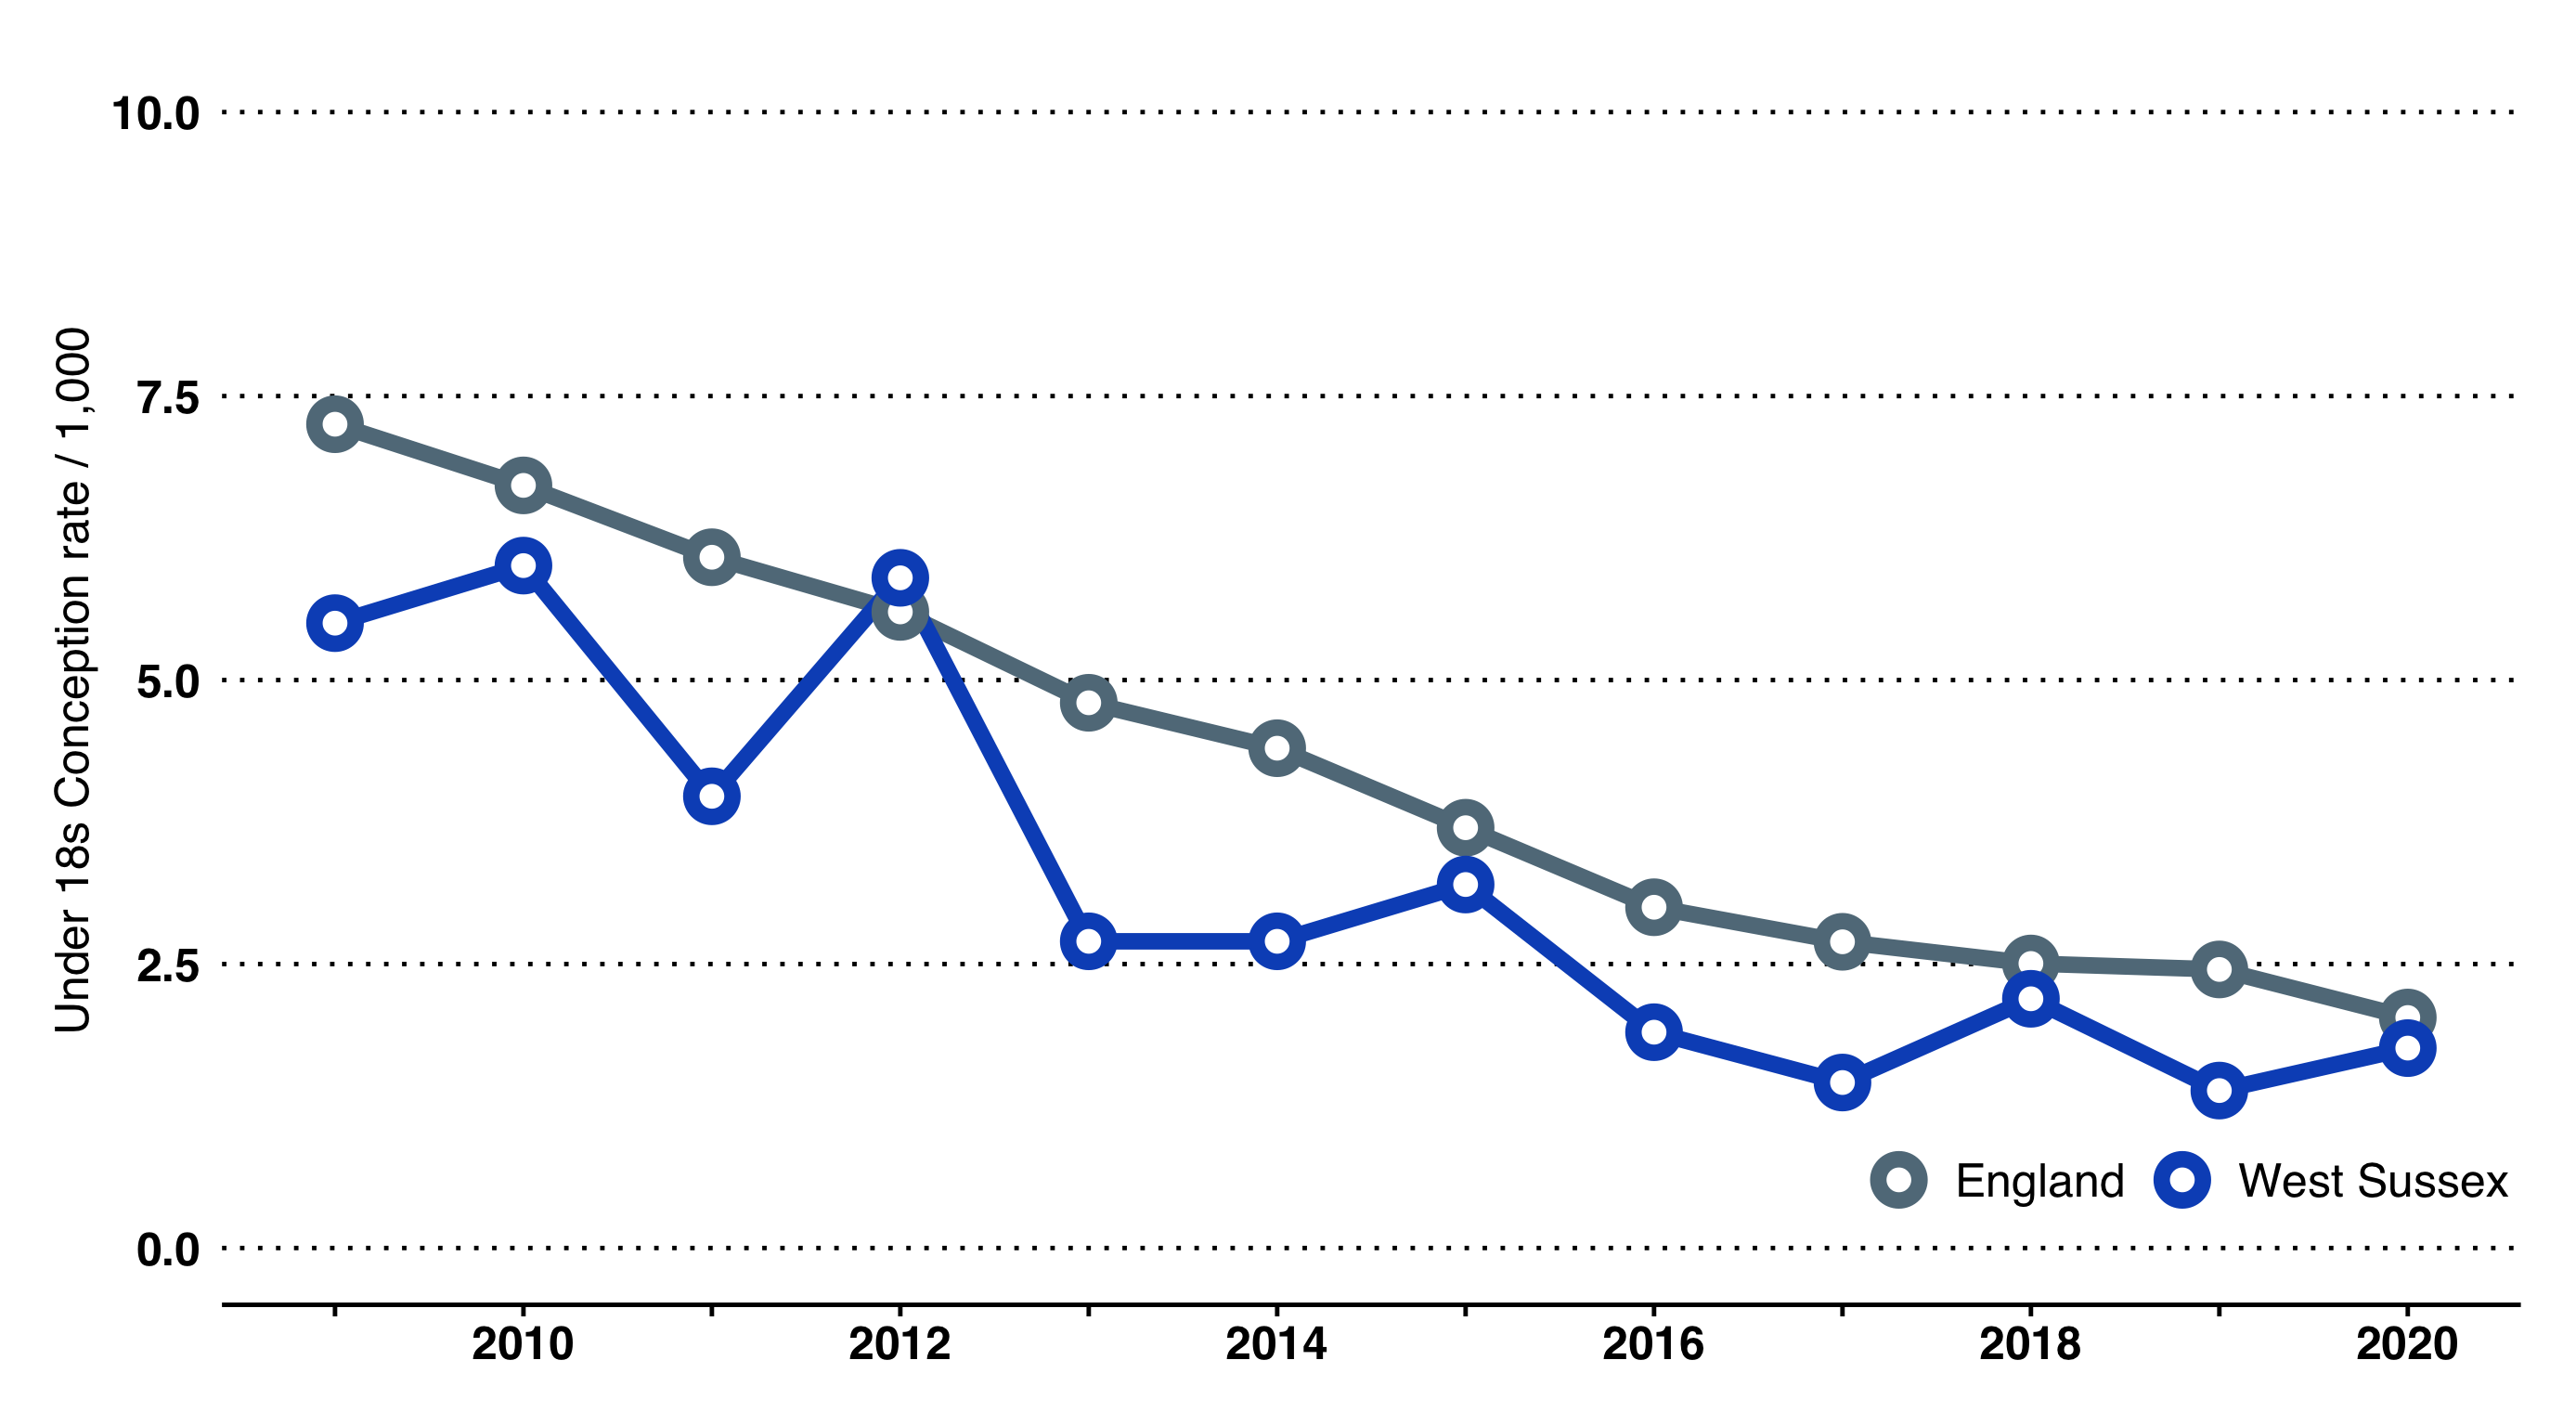
\includegraphics[width = \linewidth]{images/u18s_conc_line.png}
\end{figure}

\begin{figure}[ht]
    \caption{The percentage of abortions undertaken in under 10 weeks has declined in recent years; after a steep fall in 2017, the percentage has risen again, and is now similar to England.}\label{fig:ab_u10wks}
    \centering
    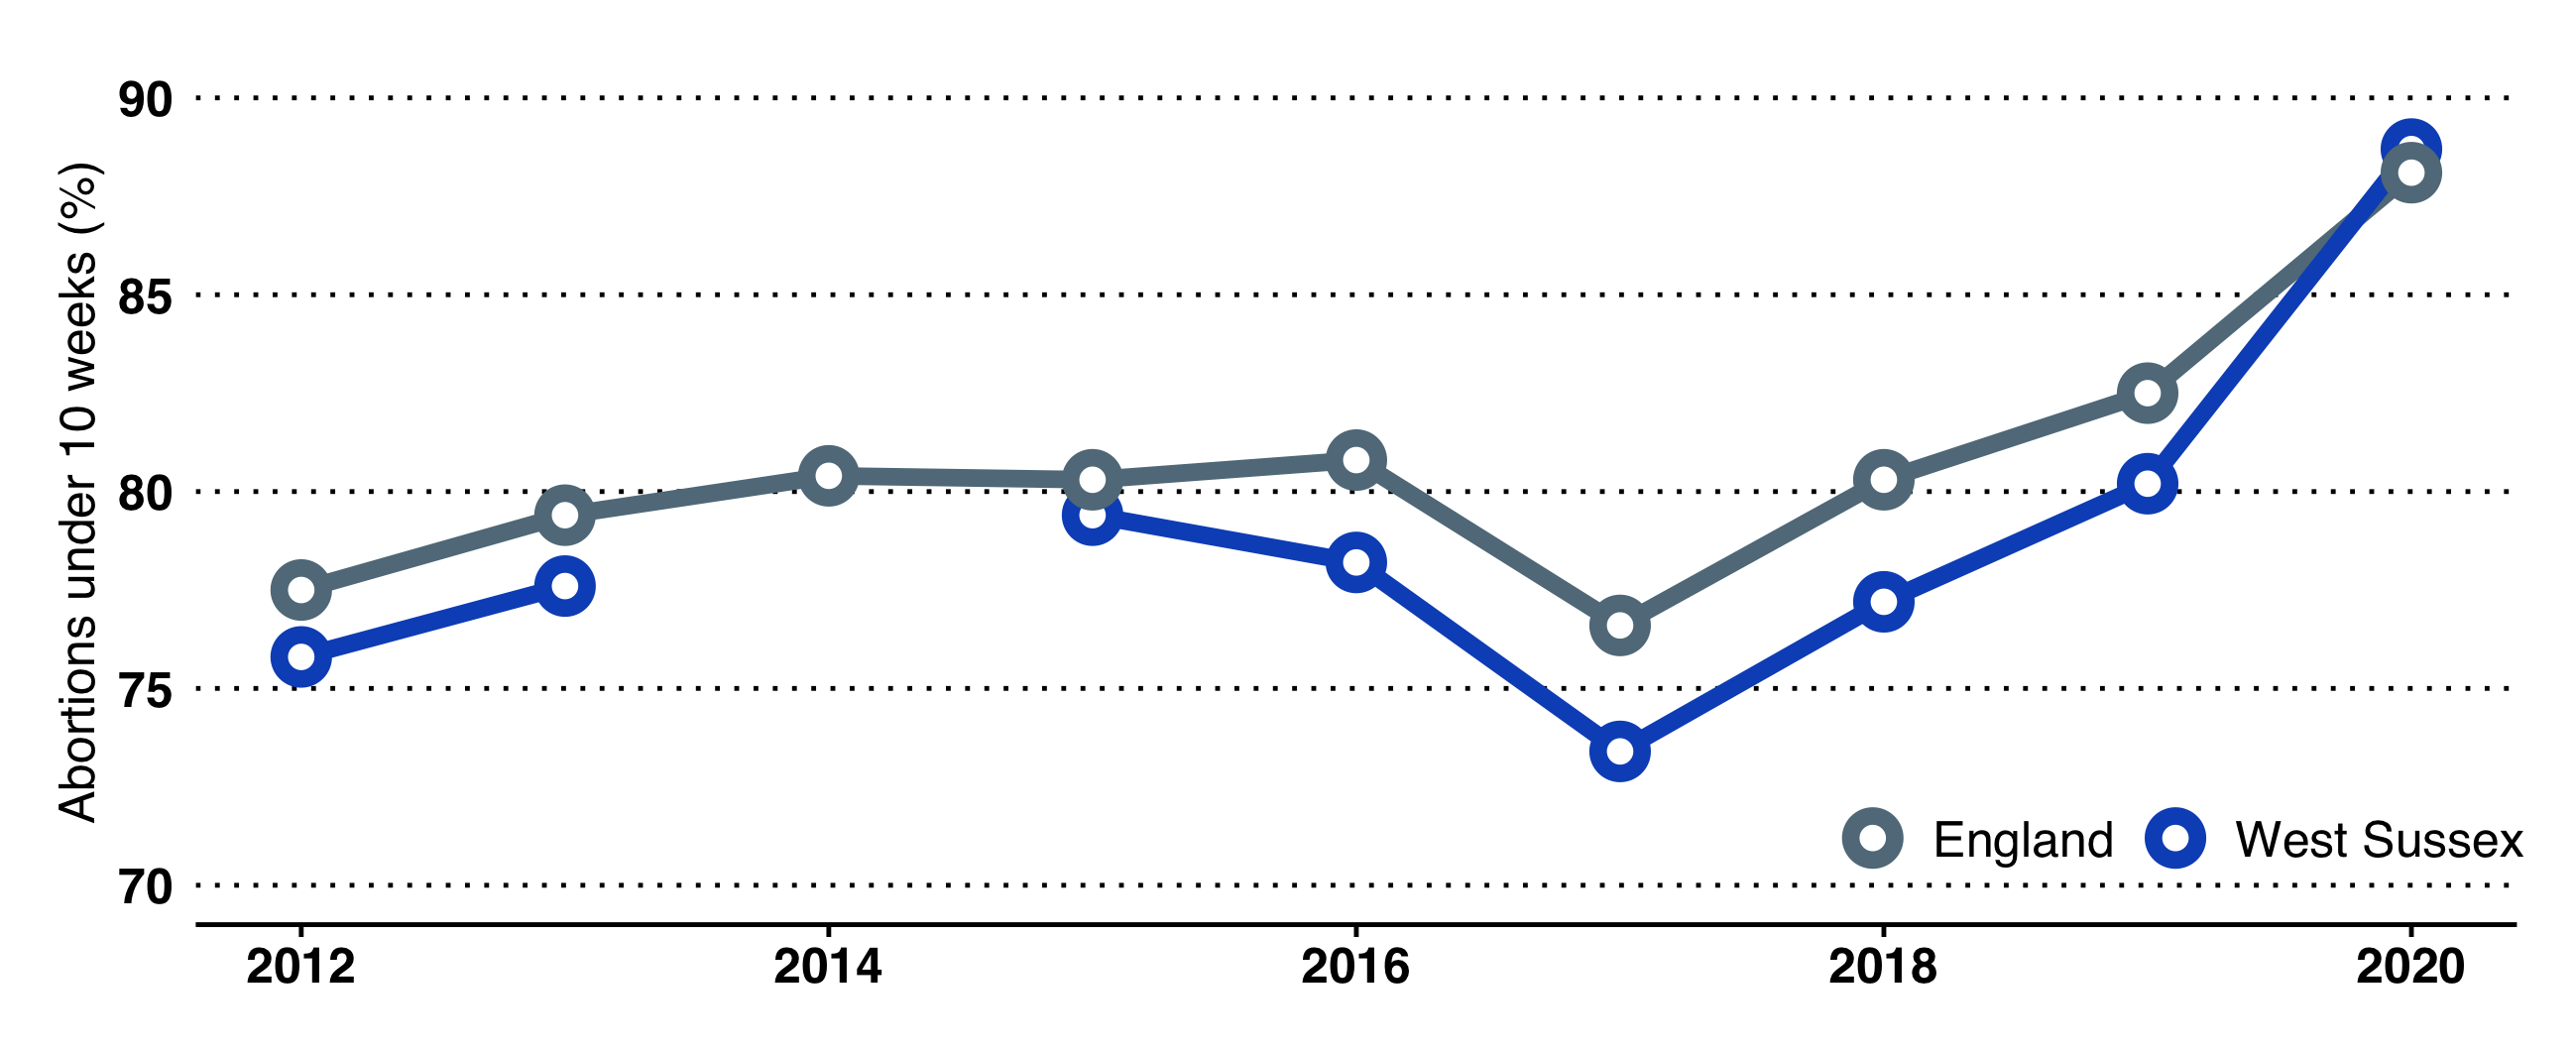
\includegraphics[width = \linewidth]{images/abortions_lt_10wks_line.png}
\end{figure}

\begin{figure}[H]
    \caption{After peaking in 2016, the percentage of repeat abortions in under-25s has fallen to the average level of previous years (around 24\%).}\label{fig:repeat_ab}
    \centering
    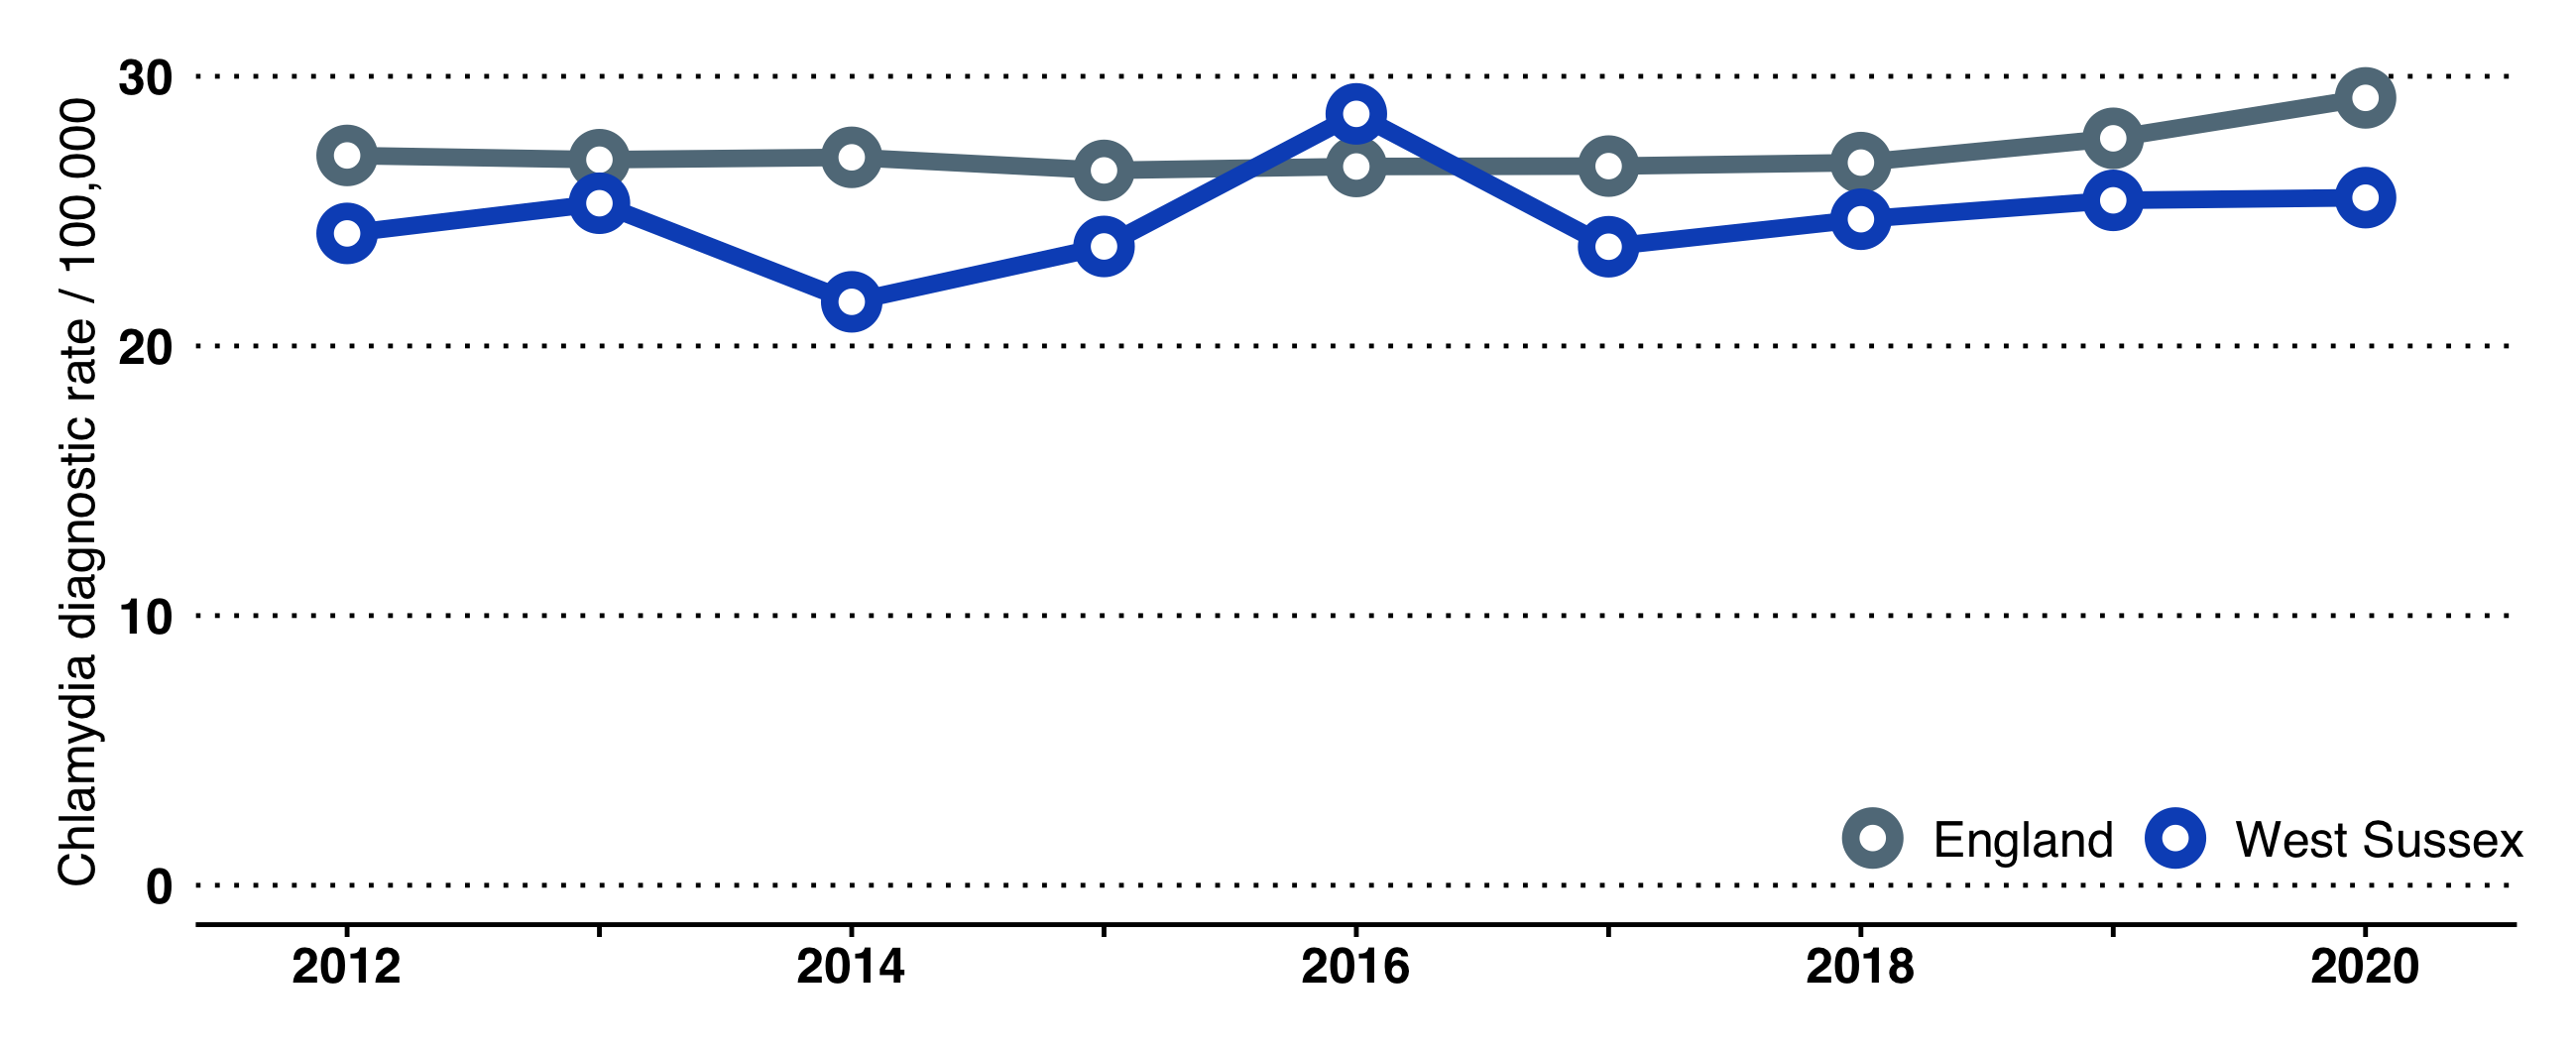
\includegraphics[width = \linewidth]{images/repeat_abortions_line.png}
\end{figure}

\paragraph{A focus on chlamydia} Chlamydia is the most common bacterial sexually transmitted infection in England and causes avoidable sexual and reproductive ill-health. Chlamydia rates are substantially higher in young adults (<25 years) than any other age group, although >25s are also at risk. 

\begin{figure}[ht]
    \caption{West Sussex Chlamydia diagnosis rate. Diagnosis rates have been been falling in West Sussex, even as rates rose in England prior to 2020.}\label{fig:ct_diagnosis}
    \centering
    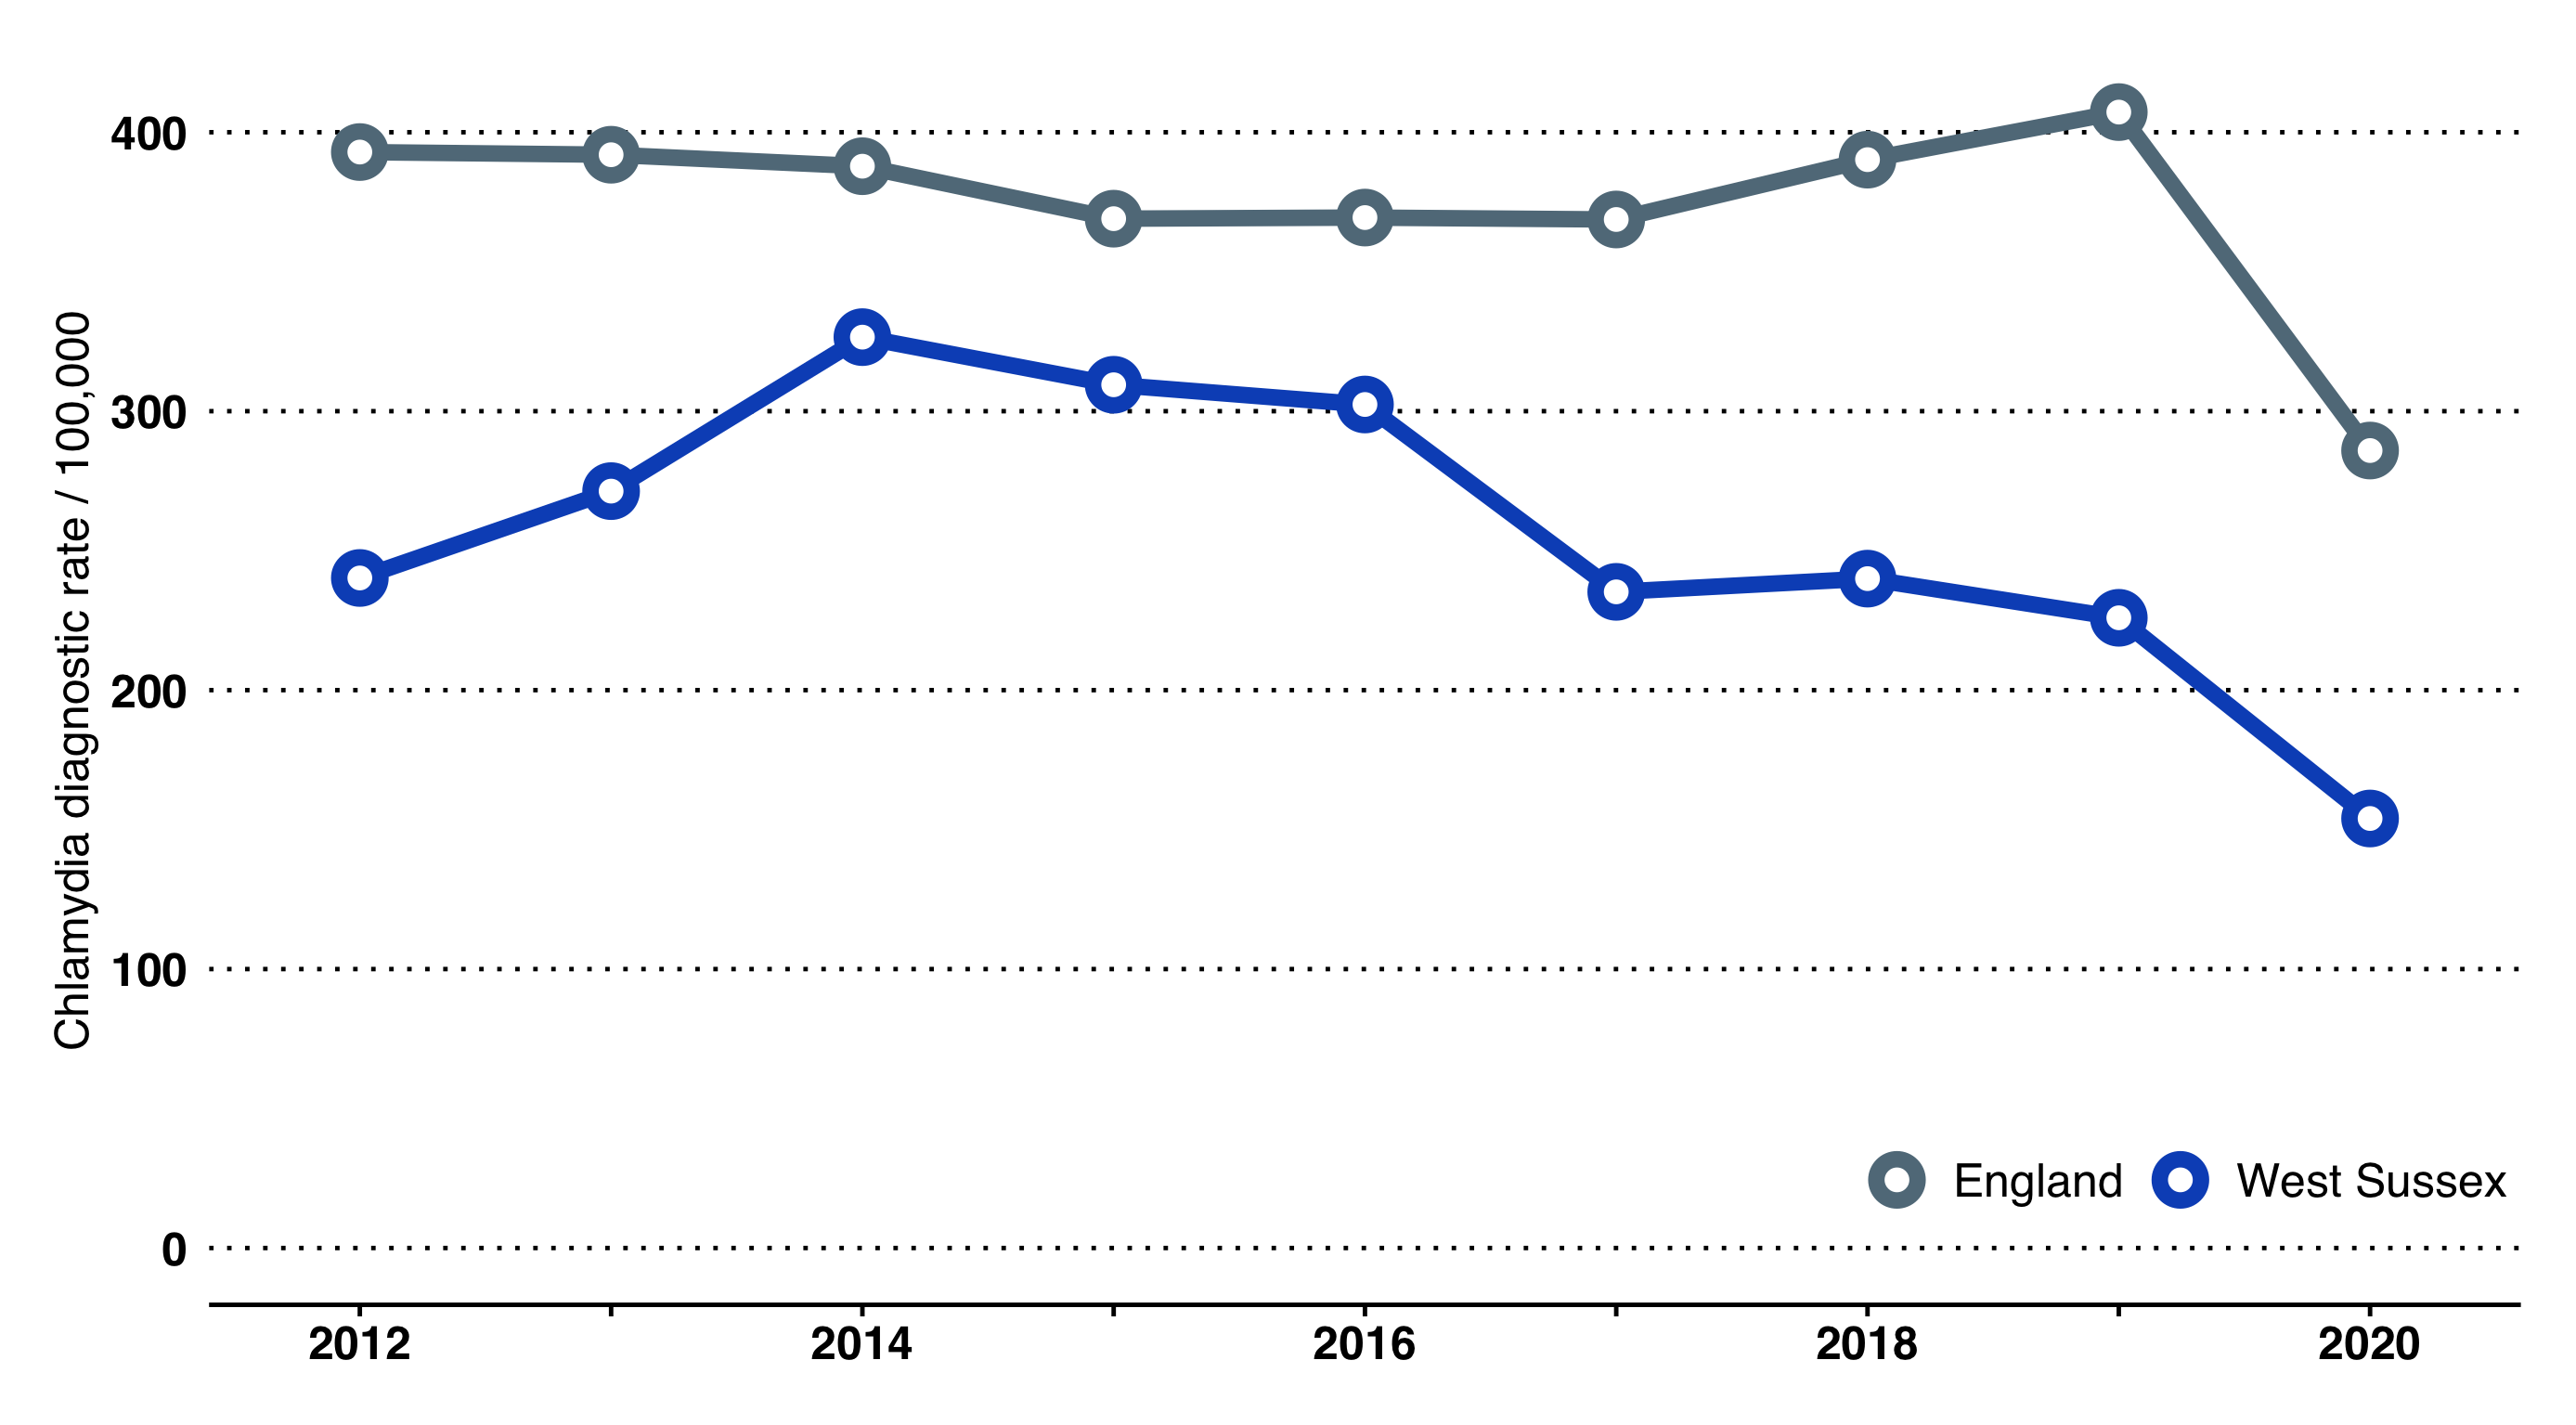
\includegraphics[width = \linewidth]{images/ct_diag_line.png}
\end{figure}

\paragraph{Screening in 15-24 year-olds} Chlamydia screening in 15-24 year-olds allows diagnosis and prompt treatment of symptomatic chlamydia infections. In addition to reducing the time in which the infection can be passed on and thus the spread of chlamydia, screening reduces the chances of an infected individual developing complications.

Screening has declined in West Sussex since 2014 and remains significantly below England in most districts and boroughs, save for Crawley which at 33.3\% of the 15-24 year-old population is signifcantly above the England average (14.3\%) and the highest proportion screened in the South East.

\begin{figure}[H]
    \caption{Percentage chlamydia screening over time and in West Sussex Local Authorities.}
    \label{figure:unpaidcarers:dabs}
    \centering
    \begin{subfigure}[b]{0.99\linewidth}
        \centering
        \caption{Annual percentage of 15-24 year olds screened  for Chlamydia, West Sussex 2012 to 2020.}\label{fig:chlamydia:p_u25_time}
        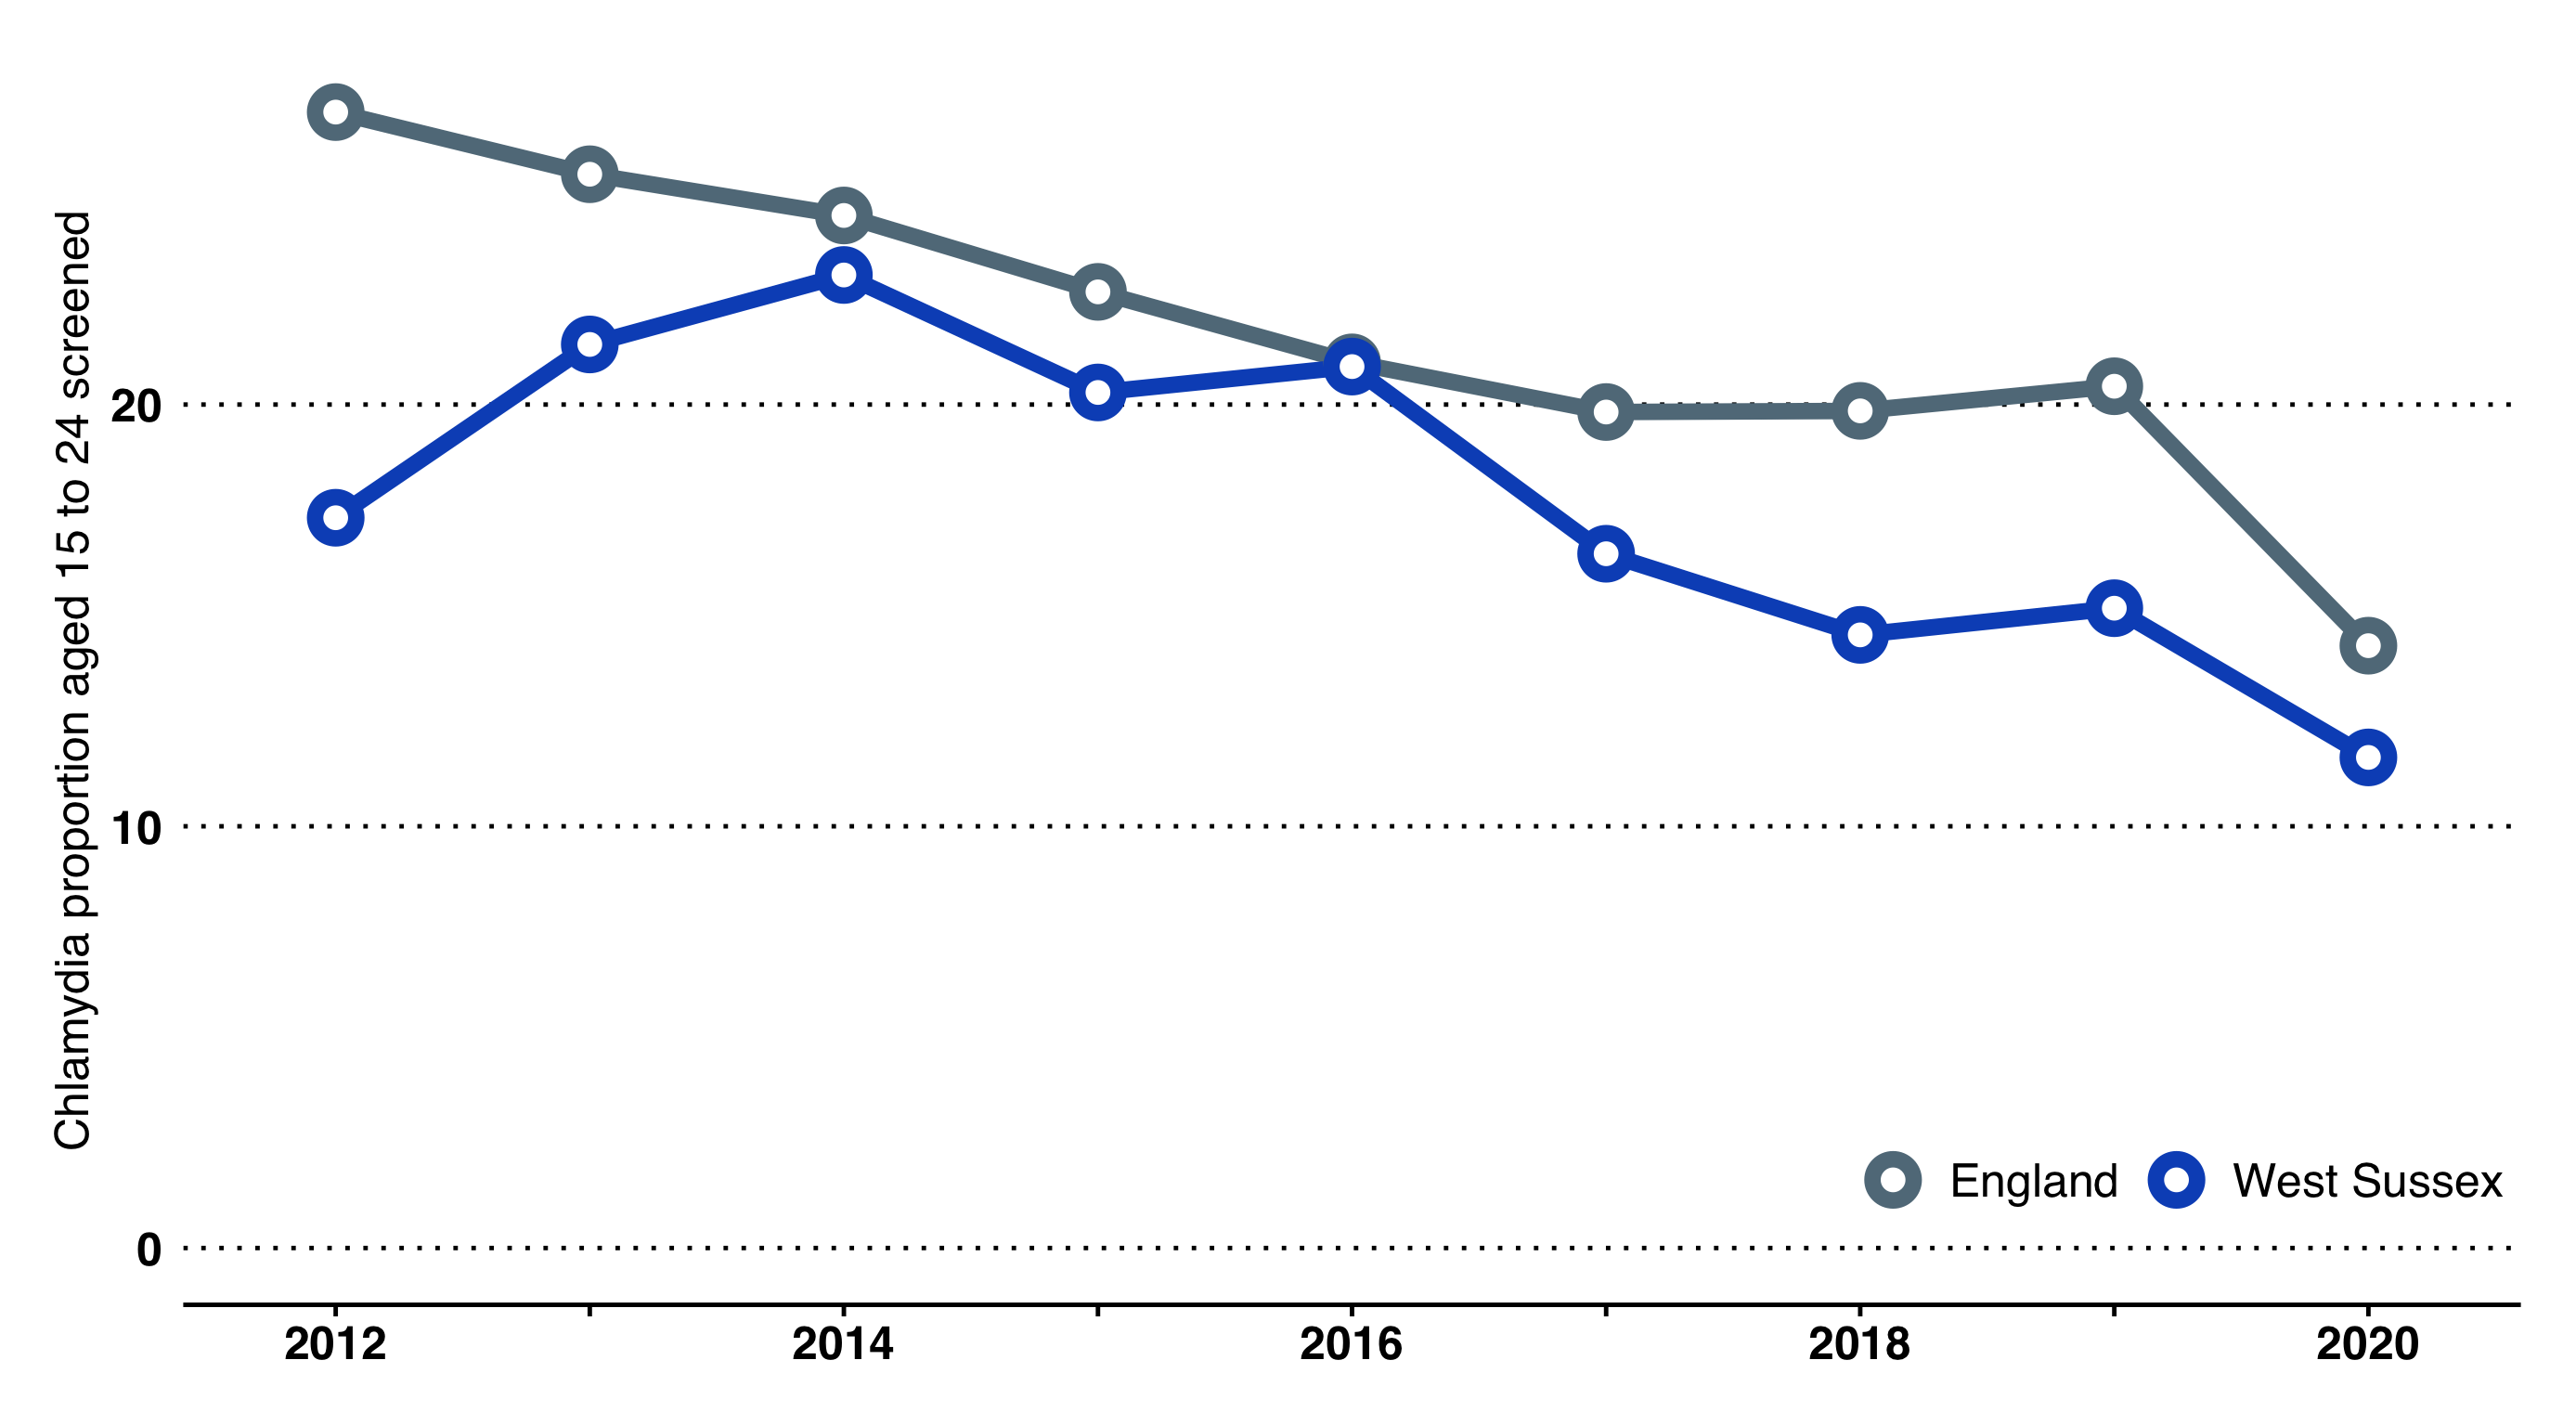
\includegraphics[width=\linewidth]{images/ct_screened_line.png}
    \end{subfigure}
    \begin{subfigure}[b]{0.99\linewidth}
        \centering
        \caption{Percentage of 15-24 year olds screened for Chlamydia, West Sussex Local Authorities 2020.}\label{fig:chlamydia:p_u25_dabs}        
        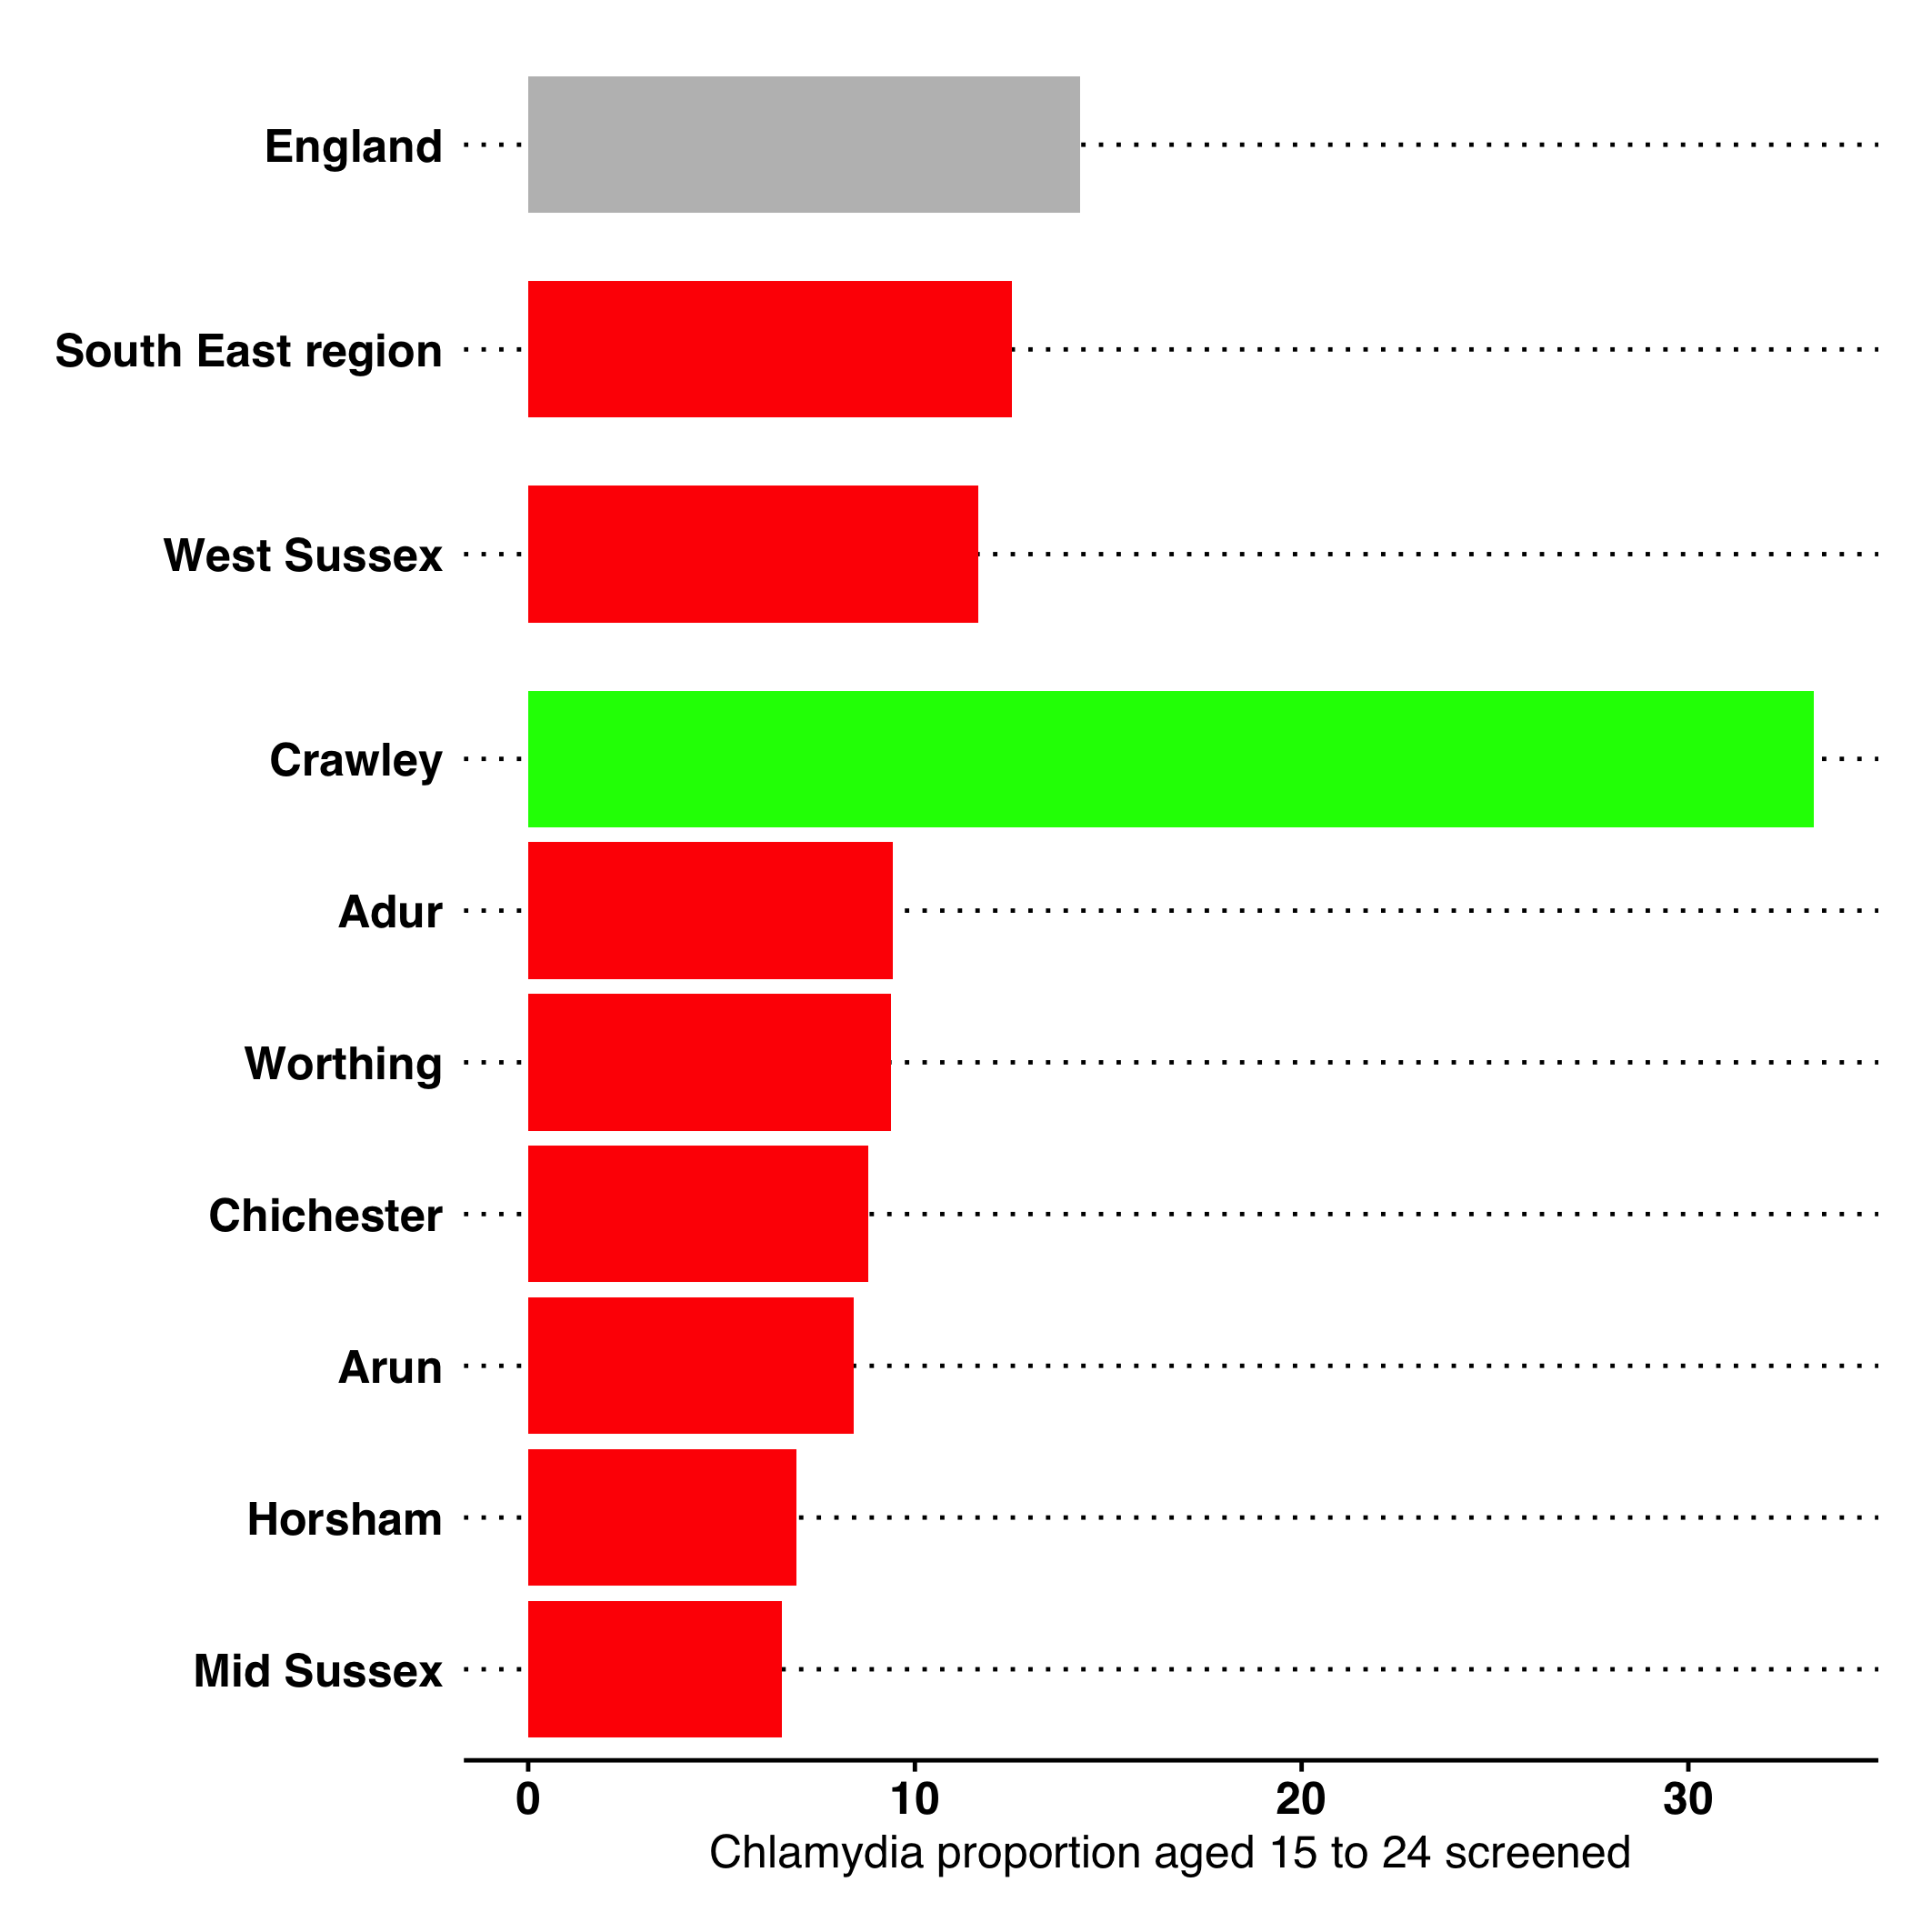
\includegraphics[width=\linewidth]{images/chlamydia_screen_yp_rag_bar.png}
    \end{subfigure}
    \vspace*{3mm}
\end{figure}



%\subsection{A Focus on HEALTH PROTECTION} 
%The West Sussex Health Protection Annual Report 2018/19 details the state of efforts to prevent and reduce ill-health in West Sussex, many of which are measures in the Public Health Outcomes Framework. This report is available on the JSNA website. For further information, contact Lobat Salehi (\url{lobat.salehi@westsussex.gov.uk}).

%\paragraph{Outbreaks}There were 246 outbreak situations or incidents in 2018/2019. Specific cases and outbreaks of note include:

%\begin{itemize}
%    \item a number of complex TB cases and incidents requiring place-based screening of contacts, including exposures in hospitals, schools and immigration removal centres.
%    \item outbreaks of seasonal flu in hospitals and care homes. GP Influenza-like illness (ILI) consultation rates peaked later in the 2018/19 season in West Sussex, at 23.4 per 100,000, than the South East and England and were lower than in the 2017/18 season.
%    \item a large Cryptosporidium outbreak relating to visits to an open farm in West Sussex during lambing season (one of four Cryptosporidium outbreaks related to open farms during lambing season across the South East in 2018/19), with a multi -agency response to investigate and manage the public health risk. 203 cases with a known link to the farm were recorded (119 confirmed, 82 probable and 2 possible).
%    \item a measles outbreak in school pupils in the Chichester area, with 29 reported cases (22 confirmed, 4 probable, 3 possible). Additional MMR vaccination catch-up clinics were offered for unvaccinated children in the area.
%\end{itemize}
   
%\subsubsection{Key challenges outlined in the 2018/19 annual report} In West Sussex, key challenges around infectious diseases are:

%\begin{itemize}
%    \item the large numbers of care homes, settings which are at risk of flu and norovirus outbreaks. Alongside the consequential impacts on the wider health economy and individuals within the care system from these outbreaks, care homes are often noted to have no or poorly effective occupational health services, resulting in low flu vaccination uptake rates for their staff 
%    \item prison and detention settings tend to out-source occupational health provision, which can often lead to delays in provision of public health measures on-site for staff, thus impacting on rapid responses to contain outbreaks
%    \item the on-going resourcing pressures on environmental health teams who enforce health protection legislation and implement controls during outbreaks, causing potential delays to managing gastro-intestinal cases and outbreaks
%    \item uptake of the two MMR vaccines by 5 years olds not reaching the 95\% target required to provide adequate herd immunity\footnote{PHOF reference D04c}, increasing the risk of widespread measles outbreaks
%    \item increasing numbers of open farms providing open days to the public during lambing season. Awareness of the required standards documented in the Industry Code of Practice is needed to reduce the risk of the spread of gastrointestinal illness
%    \item higher rates of TB in the Crawley area compared with the South-East and England rates (See Table~\ref{tab:wa:tb} on page~\pageref{tab:wa:tb}).
%\end{itemize}

%\begin{table}
%    \caption{TB Rates (per 100,000 population)}
%    \centering
%    \begin{tabular}{llll}
%    \toprule
%    \ & Crawley & South East & England \\
%    \midrule
%    2017 & 12.5 & 6.2 & 9.1 \\
%    2016 & 20.6 & 6.5 & 10.1 \\
%    \bottomrule
%    \end{tabular}
%    \label{tab:wa:tb}
%\end{table}

\subsection{Screening}
\subsubsection{Flu jabs - for at risk groups} Coverage of flu vaccinations for at-risk groups\footnote{PHOF reference D05. These are individuals from age six months to under 65 years, excluding otherwise 'healthy' pregnant women and carers.} was 56.7\% in 2020/21. Coverage has been increasing year on year since 2015/16, remains above the England rate and is now above the $\geq$55\% benchmark.

\begin{figure}[htp]
    \caption{Flu vaccination coverage - over 65s}
    \centering
    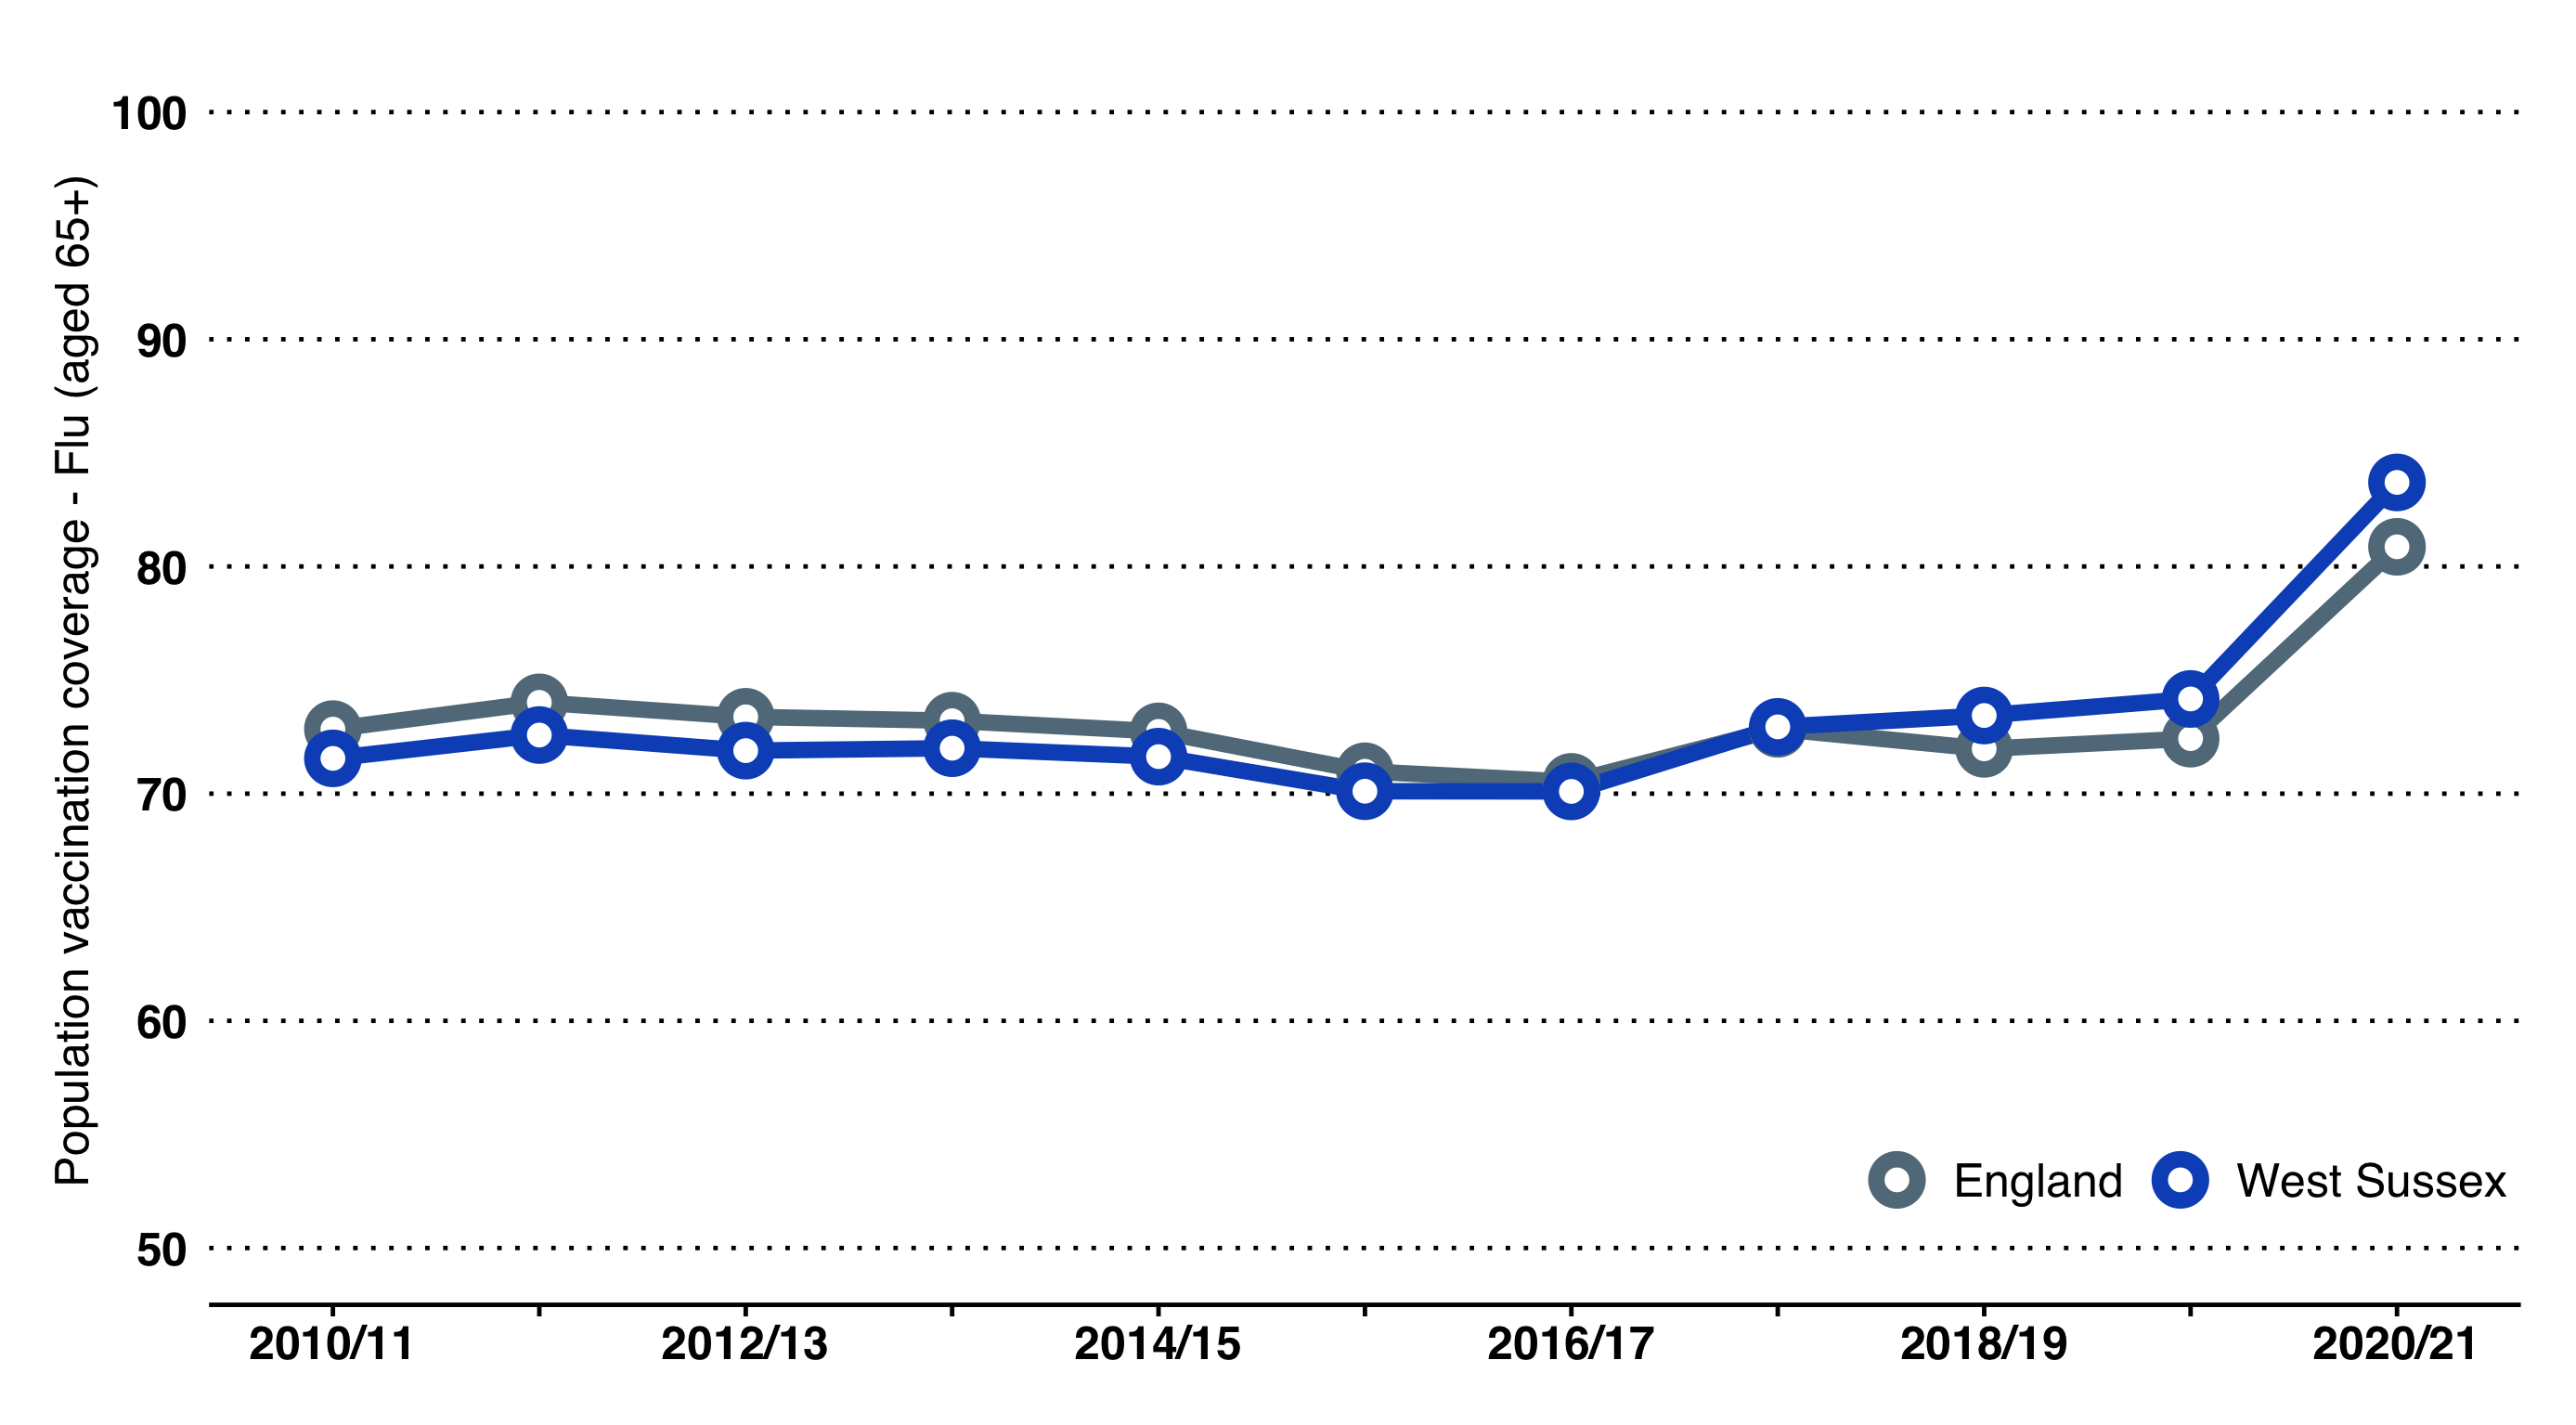
\includegraphics[width=\linewidth]{images/65over_vaccine_flu.png}
    \label{fig:flu_vax_coverage}
\end{figure}

Flu vaccinations for frontline healthcare workers involved in direct patient care increased nationally from 2017/18 to 2018/19, although there is variation above and below the 75\% target between the NHS Foundation Trusts serving the population of West Sussex.\footnote{Note: These figures have not been updated since 2018/19.}

\subsubsection{NHS Health Checks} For NHS Health Checks, West Sussex continues to perform poorly compared with England on all outcome measures\footnote{PHOF references C26a, C26b and C26c}:

\begin{itemize}[noitemsep]
    \item The cumulative percentage of the eligible population aged 40-74 offered an NHS Health Check in the five year period 2016/17 - 2020/21 was 60.4\%.
    \item The cumulative percentage of the eligible population aged 40-74 offered an NHS Health Check who received an NHS Health Check in the five year period 2016/17 - 2020/21 was 35.2\%, a decrease on the previous five year period.
    \item The cumulative percentage of the eligible population aged 40-74 who received an NHS Health Check in the five year period 2014/15 - 2018/19 was 21.3\%.
\end{itemize}


\subsubsection{Non-Cancer Screening}
% Have removed the plot of coverage over time as figures are a little wild.
\begin{figure}[ht]
    \caption[Abdominal Aortic Aneurysm screening coverage]{{\bf Abdominal Aortic Aneurysm screening coverage} The screening coverage rate at county-level for abdominal aortic aneurysm (PHOF reference C25a) was 76.7\% in 2020/21, compared to 55.0\% in England overall. Coverage in all West Sussex local authorities is higher than the South East and England.}
    \label{figure:aaa:screening}
    \centering
    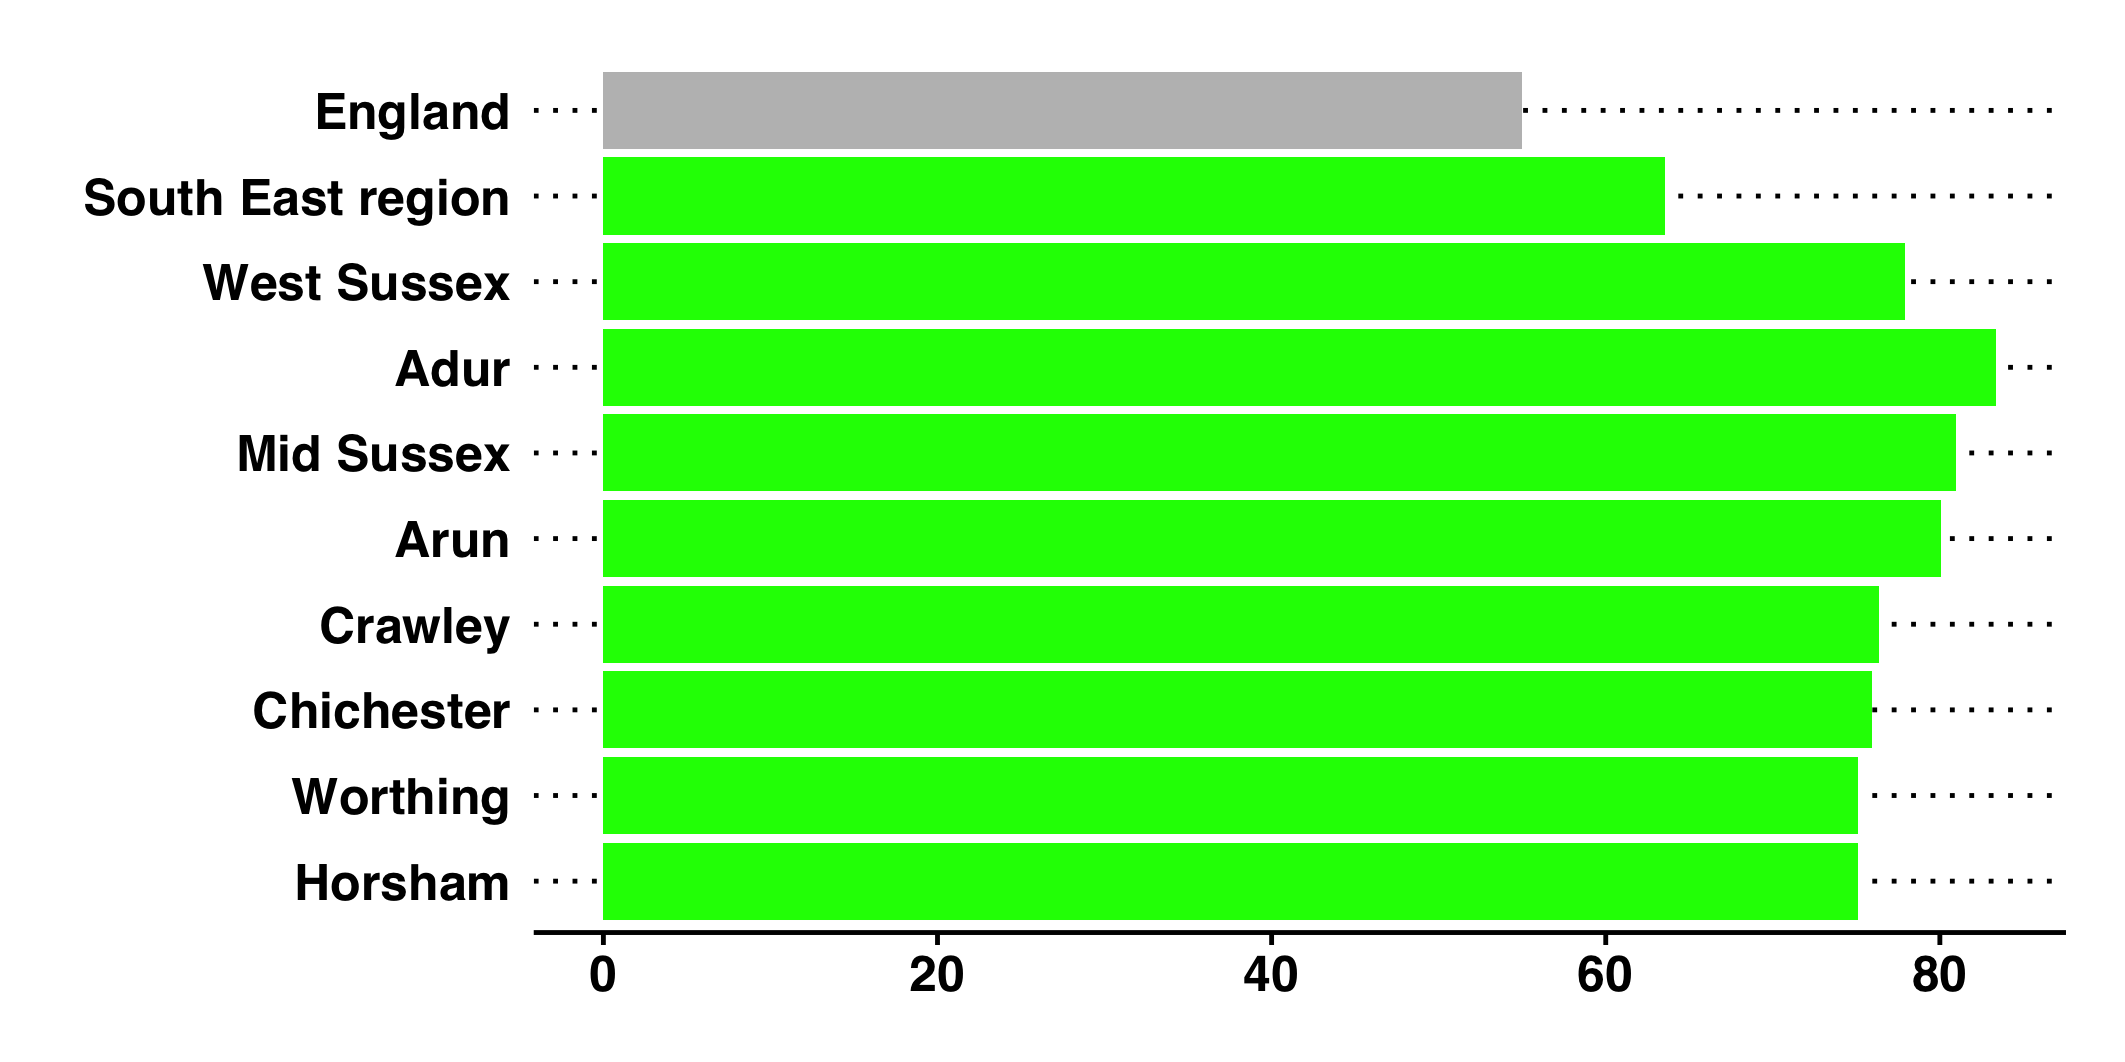
\includegraphics[width=\linewidth]{images/aaa_rag_bar.png}
\end{figure}

\paragraph{Diabetic Eye screening uptake}At the time of writing, only regional figures were available for the uptake of routine digital screening events for diabetic eye\footnote{PHOF reference C25b}. In the south east uptake was 79.2\% in 2020/21, comparing favourably to the England rate.

However this figure is lower than past coverage in West Sussex (e.g. 87.5\% uptake rate in 2018/19), indicating the disruptive effect of the pandemic on preventative screening efforts.



\subsubsection{Cancer Screening Programmes}
At county-level, overall take-up rates of screening programmes are good, comparing favourably with England and in line with rates in statistical neighbours (Figure~\ref{fig:cancer-screening}). However, there is variation between the West Sussex local authorities, with notably low rates in Crawley. All relate to 2020/21\footnote{Cervical cancer screening, PHOF reference C24b. Breast cancer screening, PHOF reference C24a. Bowel cancer screening, PHOF reference C24d.}.

% Might need to go back and make the RAG bar charts a bit taller - will see how it looks in the print out

\begin{figure*}
    % At county-level, overall take-up rates of screening programmes are good, comparing favourably with England and in line with rates in statistical neighbours. However, there is variation between the West Sussex local authorities, with notably low rates in Crawley. All relate to 2020/21.\\
    \caption[Cancer screening rates in West Sussex and its consituent lower tier local authorities.]{The screening rate at county-level for {\bf cervical cancer} (in women aged 25-49 years) is 72.2\% (Crawley, 67.3\%). Uptake had reached a 20-year low in 2018, although promotional campaigns have contributed to increases since. For {\bf breast cancer}, the screening rate at county-level is 73.1\% (Screening rates are higher than England for all districts and boroughs in West Sussex, though rates are lowest in Crawley, 65.0\%). Recent issues with the West Sussex breast programme's round length may explain the decline in screening coverage. The screening rate at county-level for {\bf bowel cancer} is 69.4\% (Crawley, 64.7\%).}\label{fig:cancer-screening}
    \vspace*{5mm}
    \centering
    \begin{subfigure}[b]{0.32\textwidth}
        \centering
        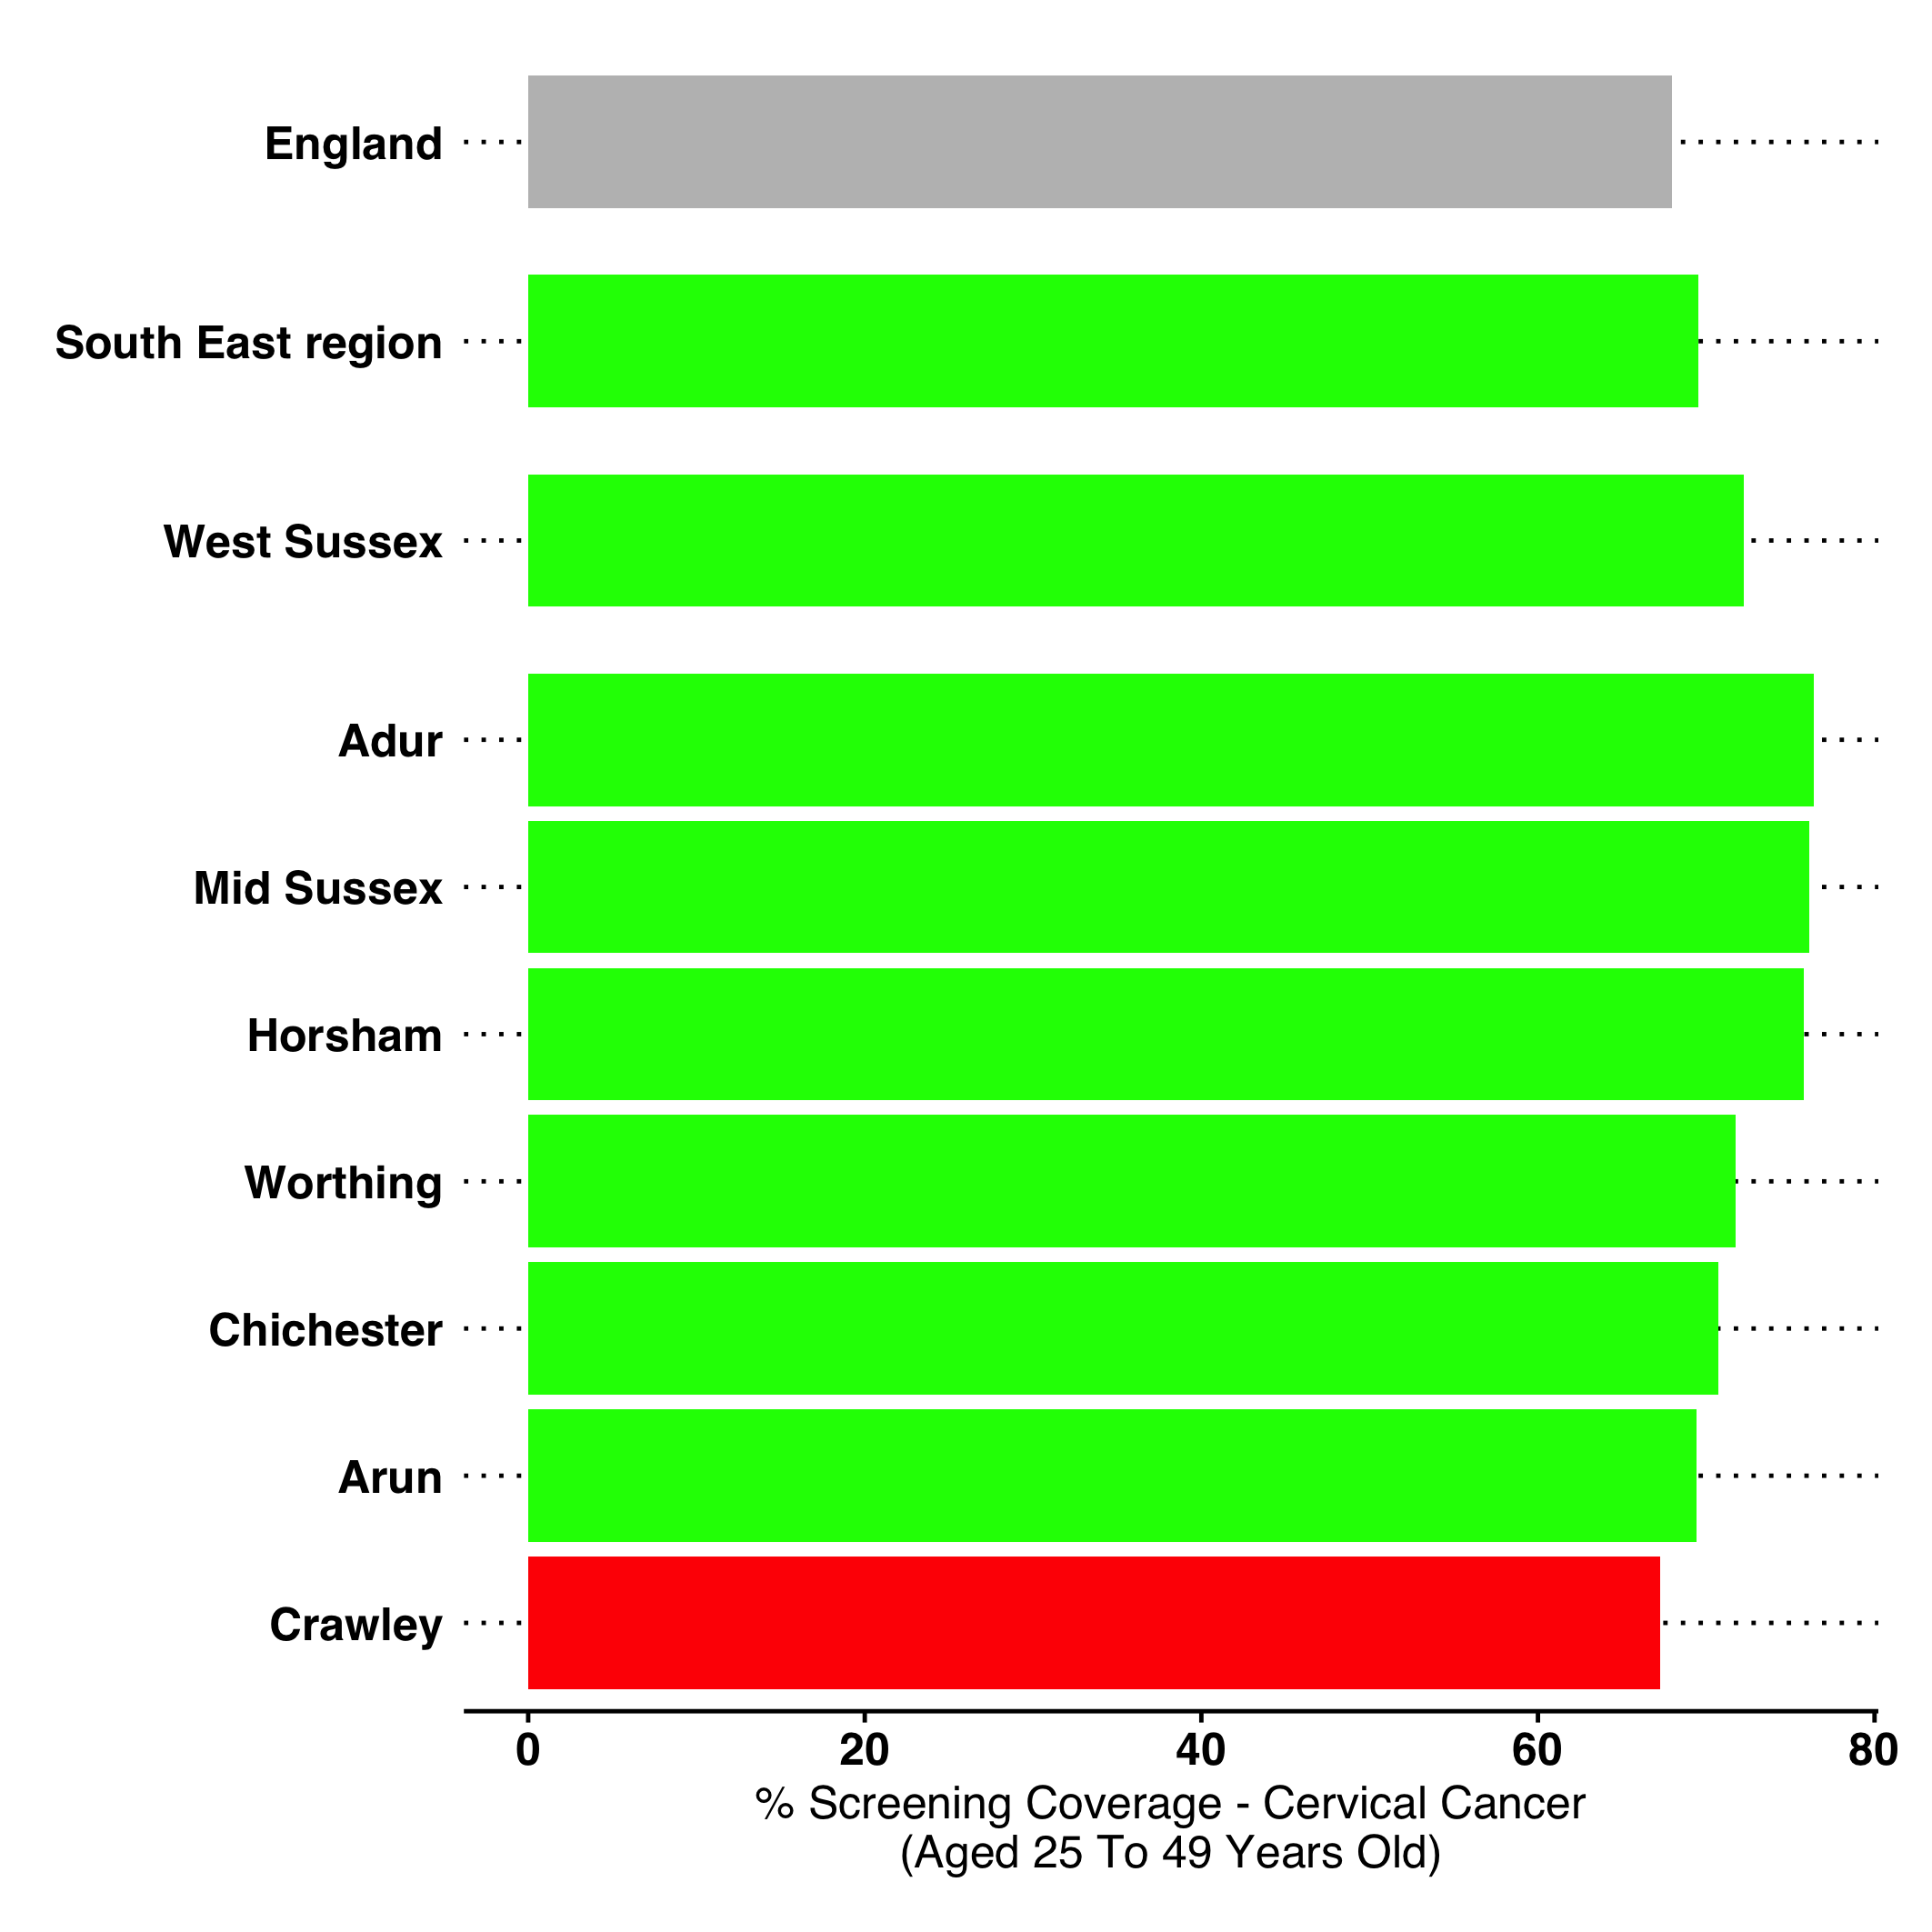
\includegraphics[width=\textwidth]{images/cervical_cancer_rag_bar.png}
        \caption{Cervical cancer screening coverage 2020/21 West Sussex Local Authorities}
        \label{fig:cervical:rag}
    \end{subfigure}
    \begin{subfigure}[b]{0.32\textwidth}
        \centering
        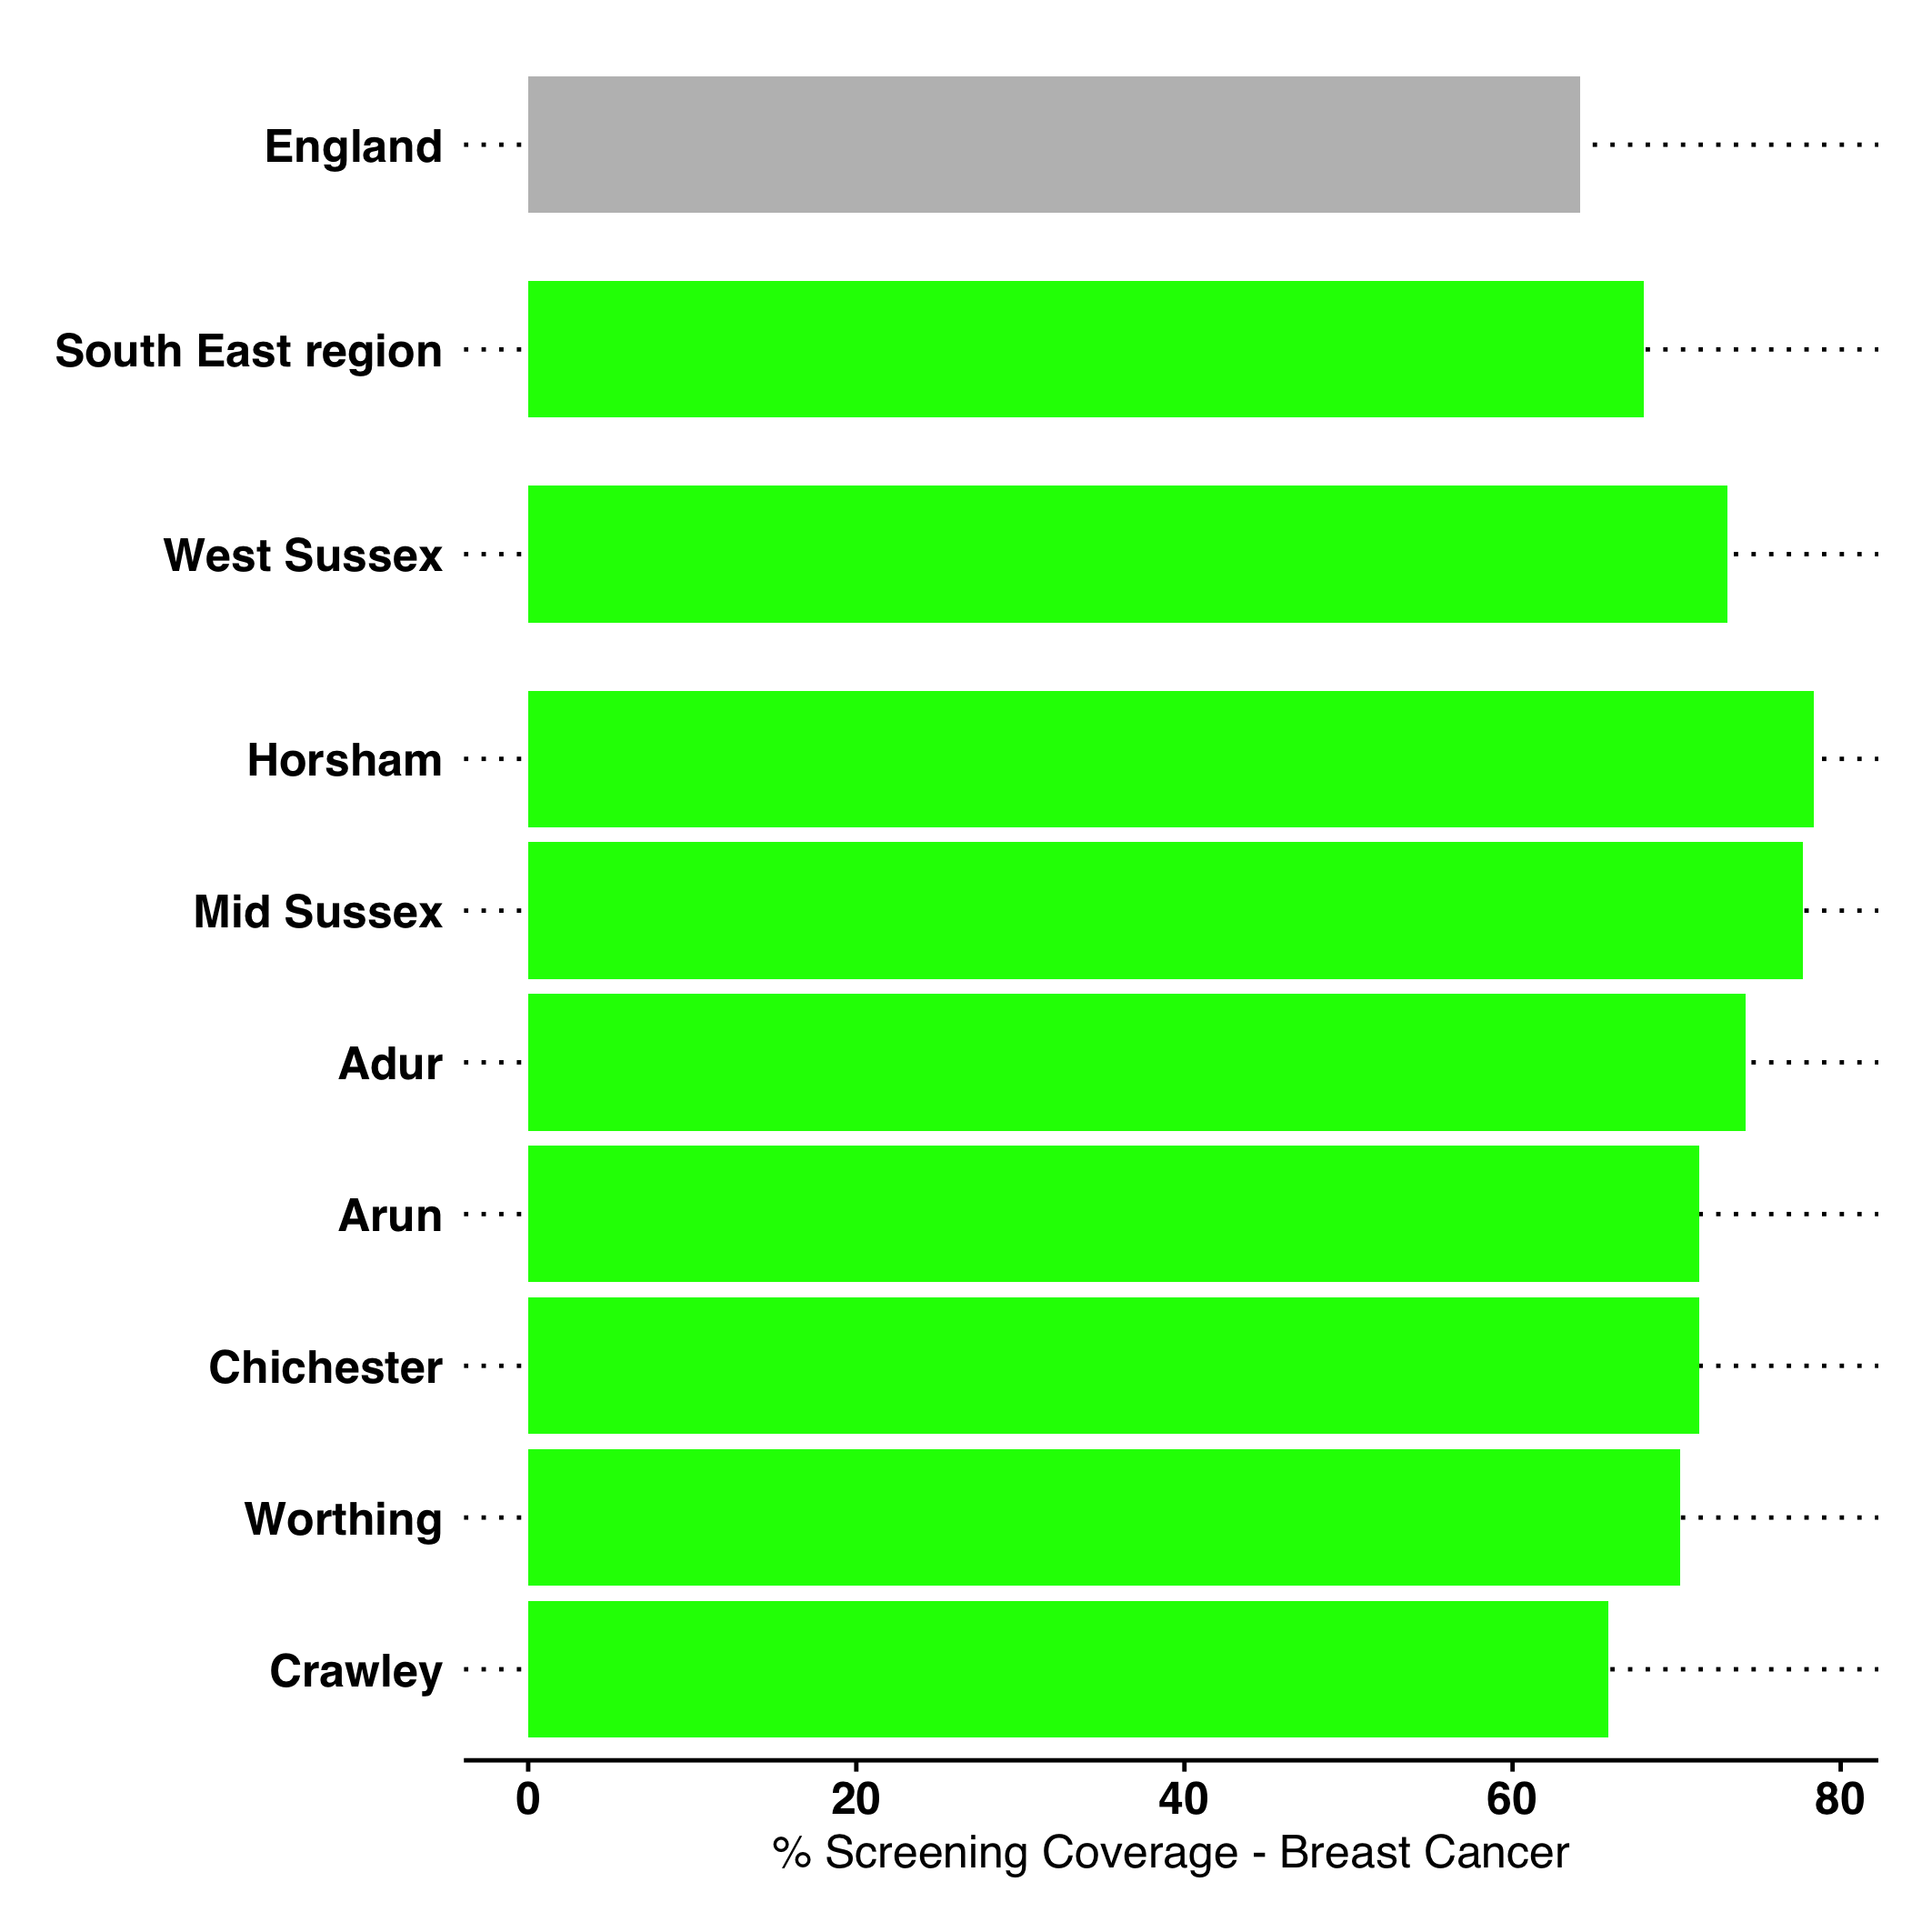
\includegraphics[width=\textwidth]{images/breast_cancer_rag_bar.png}
        \caption{Breast cancer screening coverage 2020/21 West Sussex Local Authorities}
        \label{fig:breast:rag}
    \end{subfigure}
    \begin{subfigure}[b]{0.32\textwidth}
        \centering
        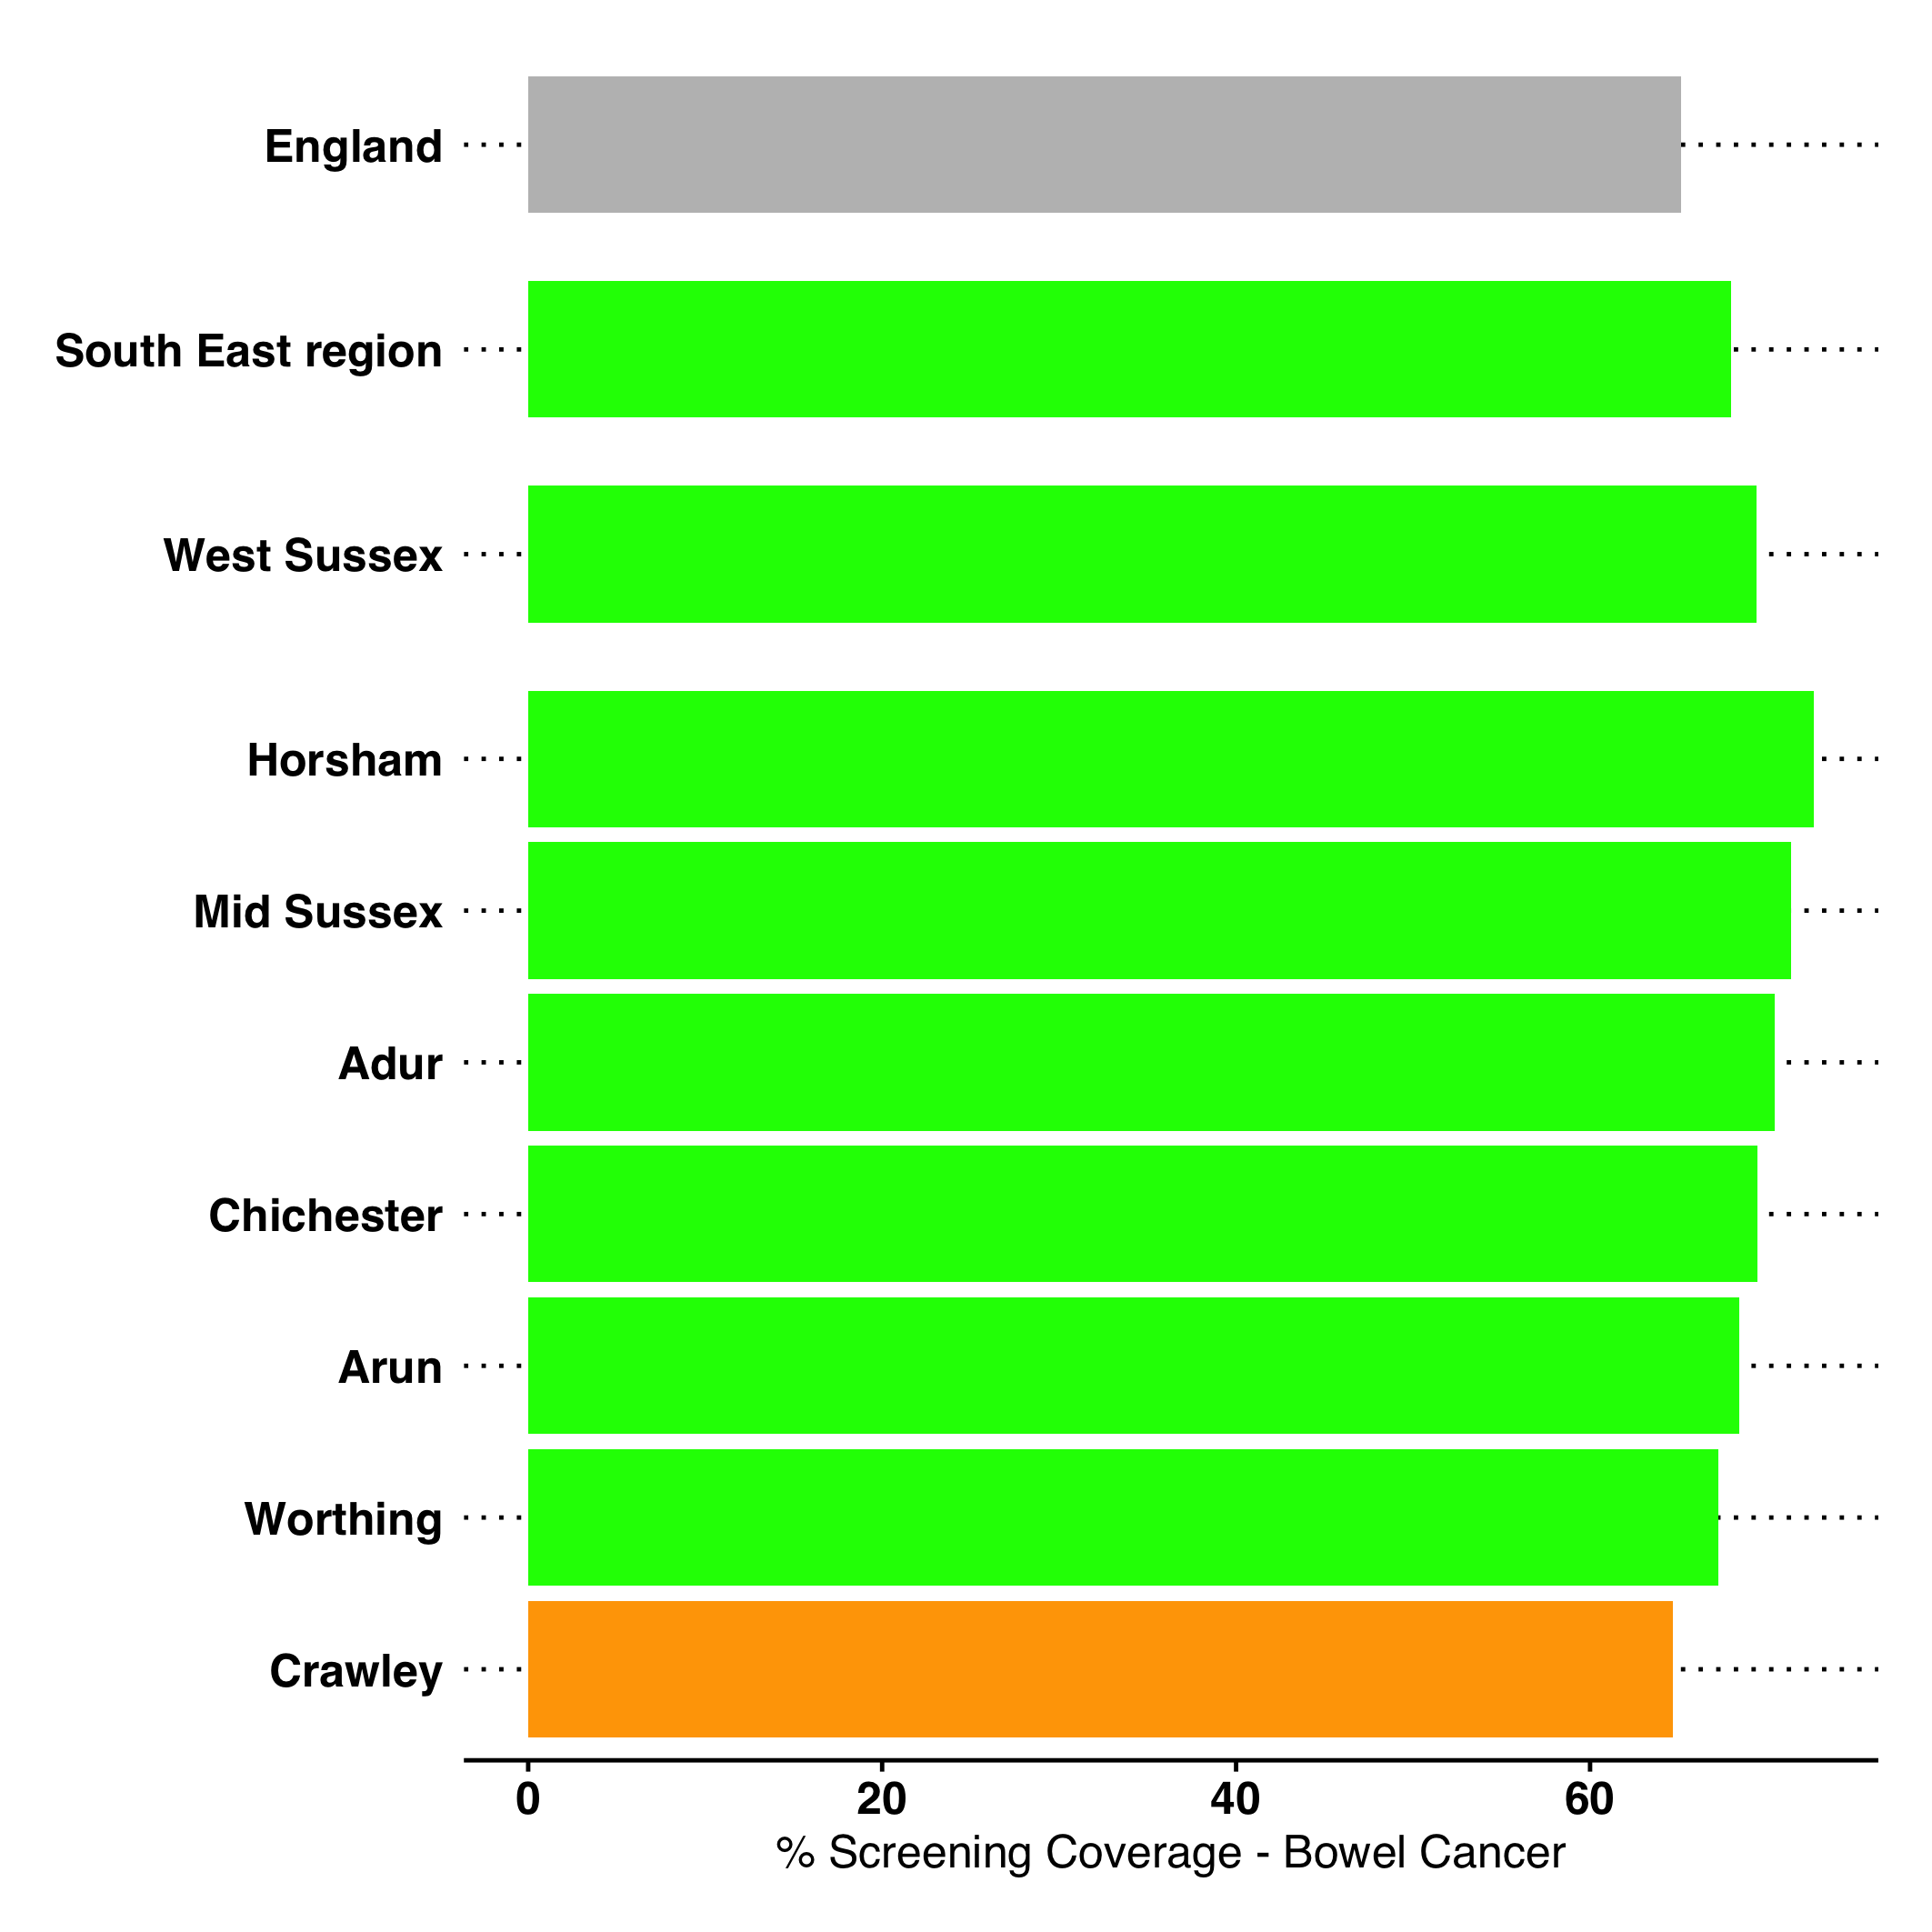
\includegraphics[width=\textwidth]{images/bowel_cancer_rag_bar.png}
        \caption{Bowel cancer screening coverage 2020/21 West Sussex Local Authorities}
        \label{fig:bowel:rag}
    \end{subfigure}
    \begin{subfigure}[b]{0.32\textwidth}
        \centering
        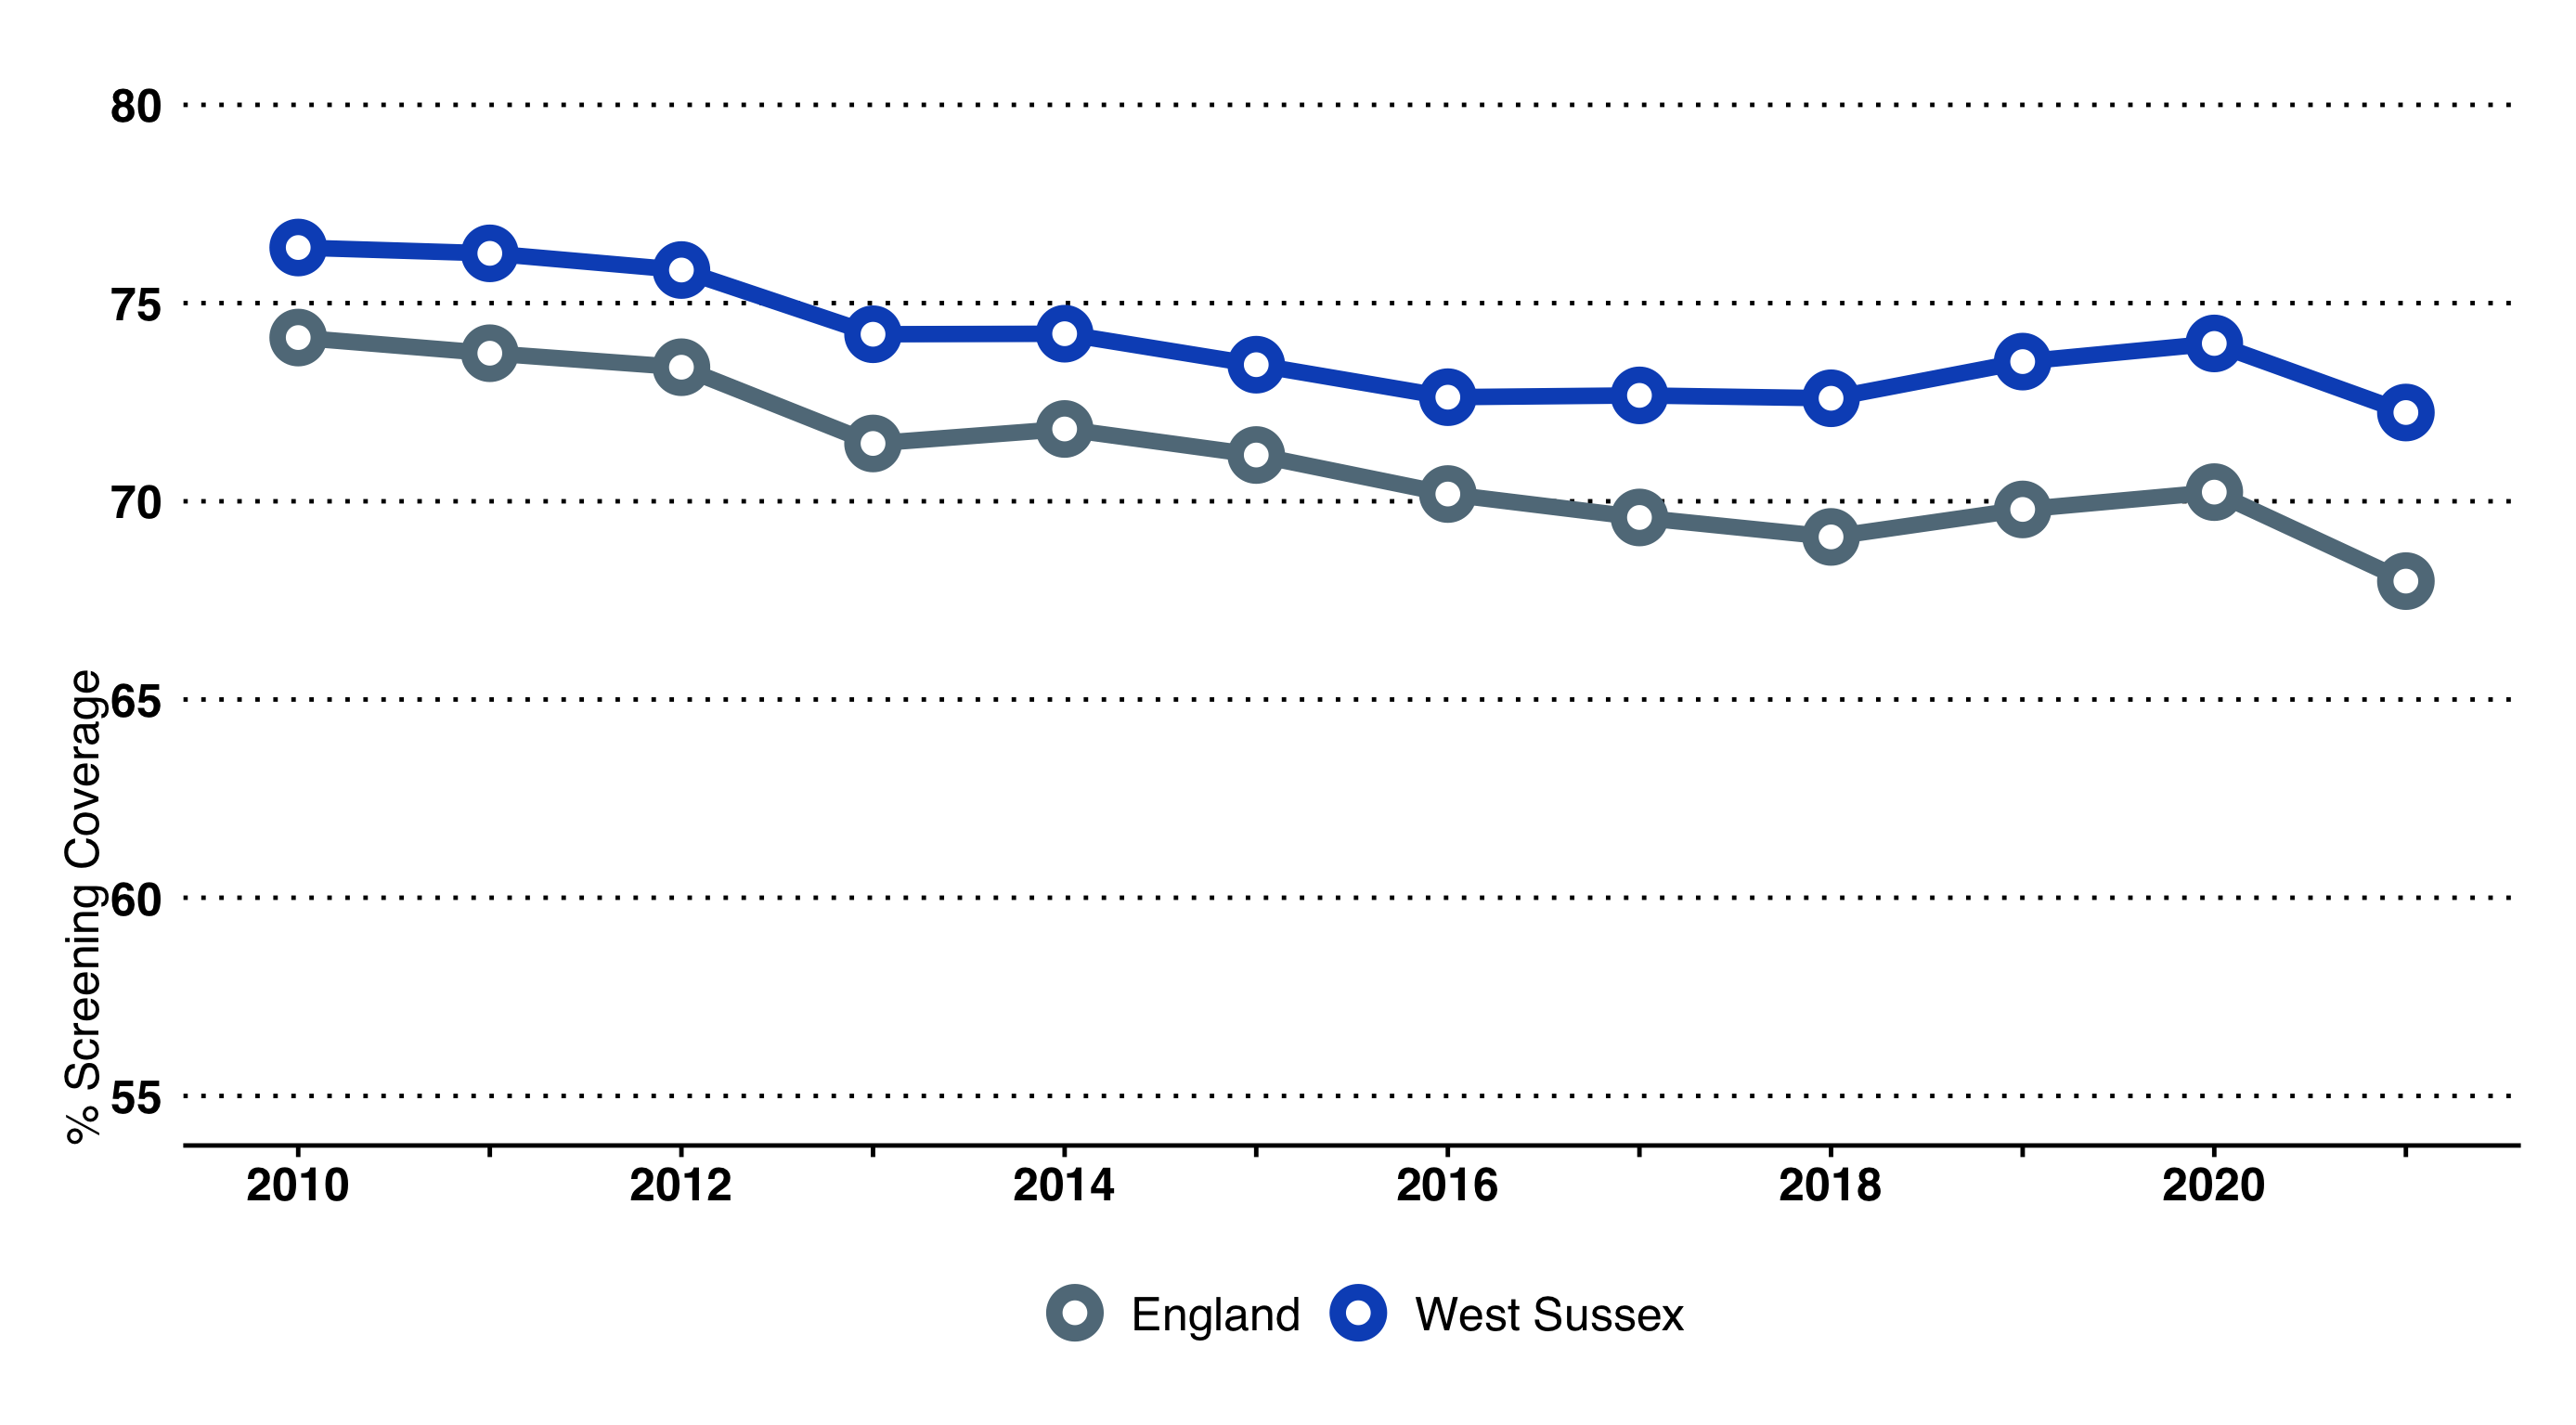
\includegraphics[width=\textwidth]{images/cervical_cancer_screening.png}
        \caption{Cervical Cancer screening coverage - West Sussex and England over time}
        \label{fig:cervical:time}
    \end{subfigure}
    \begin{subfigure}[b]{0.32\textwidth}
        \centering
        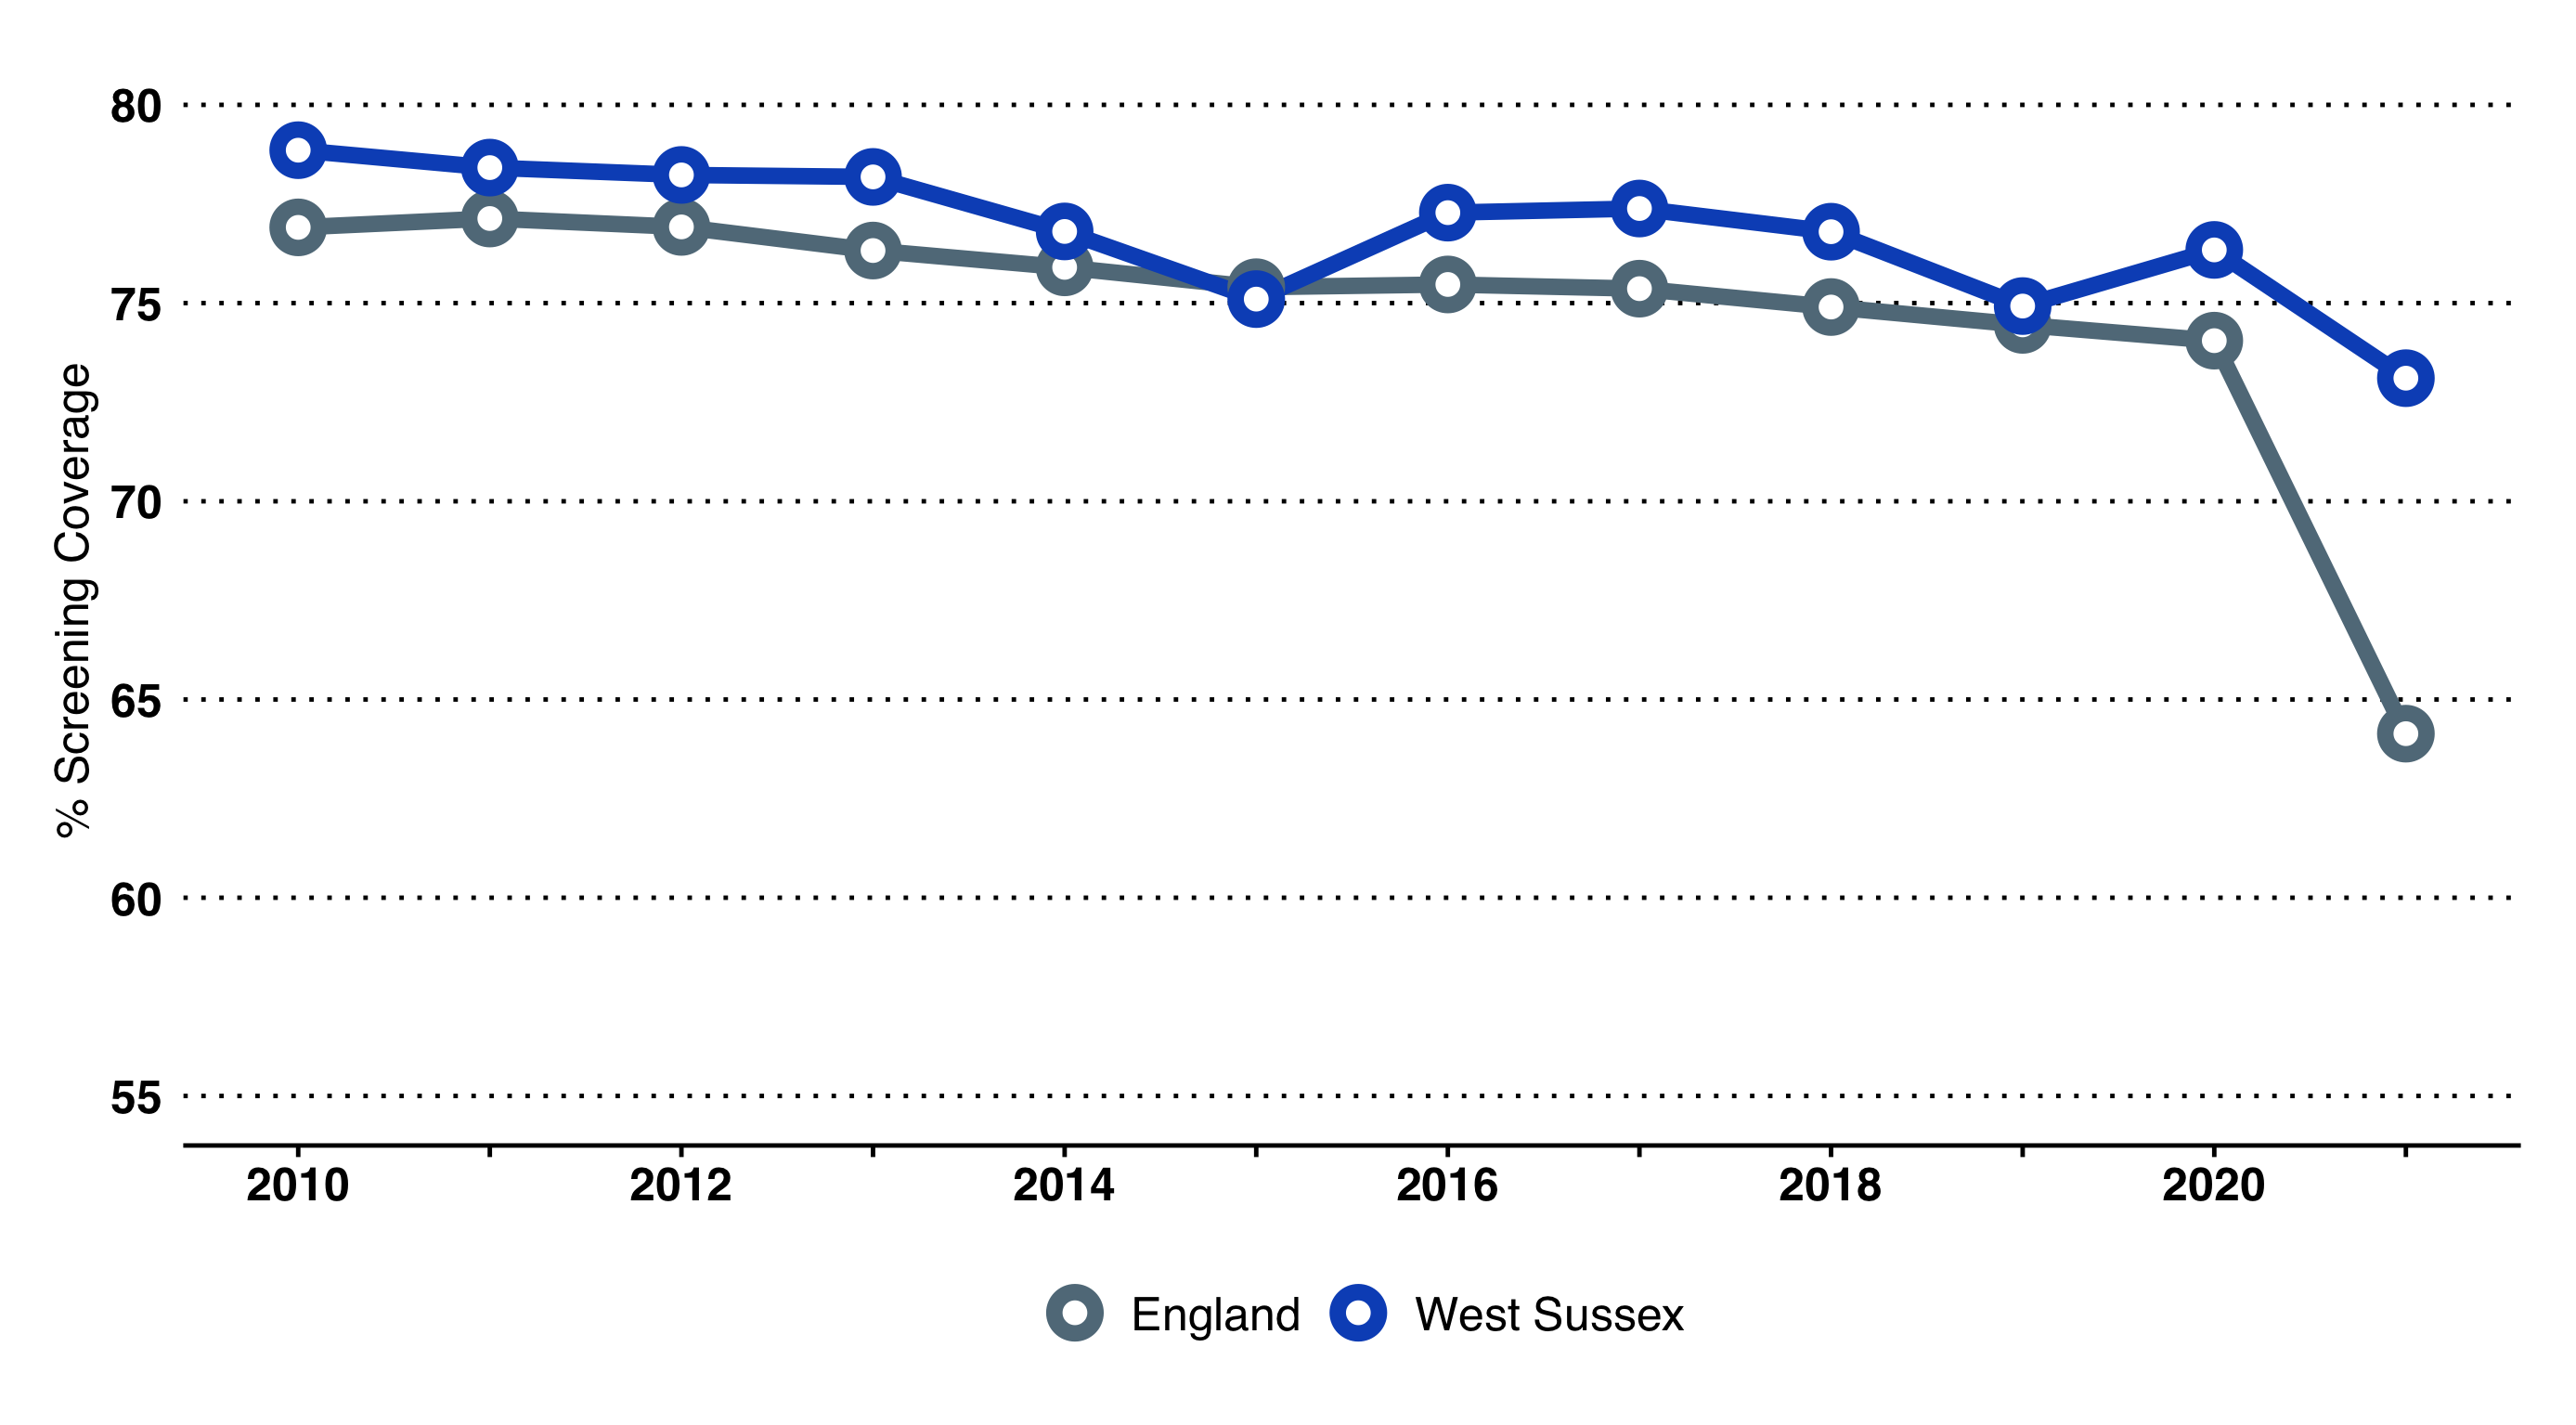
\includegraphics[width=\textwidth]{images/breast_cancer_screening.png}
        \caption{Breast Cancer screening coverage - West Sussex and England over time}
        \label{fig:breast:time}
    \end{subfigure}
    \begin{subfigure}[b]{0.32\textwidth}
        \centering
        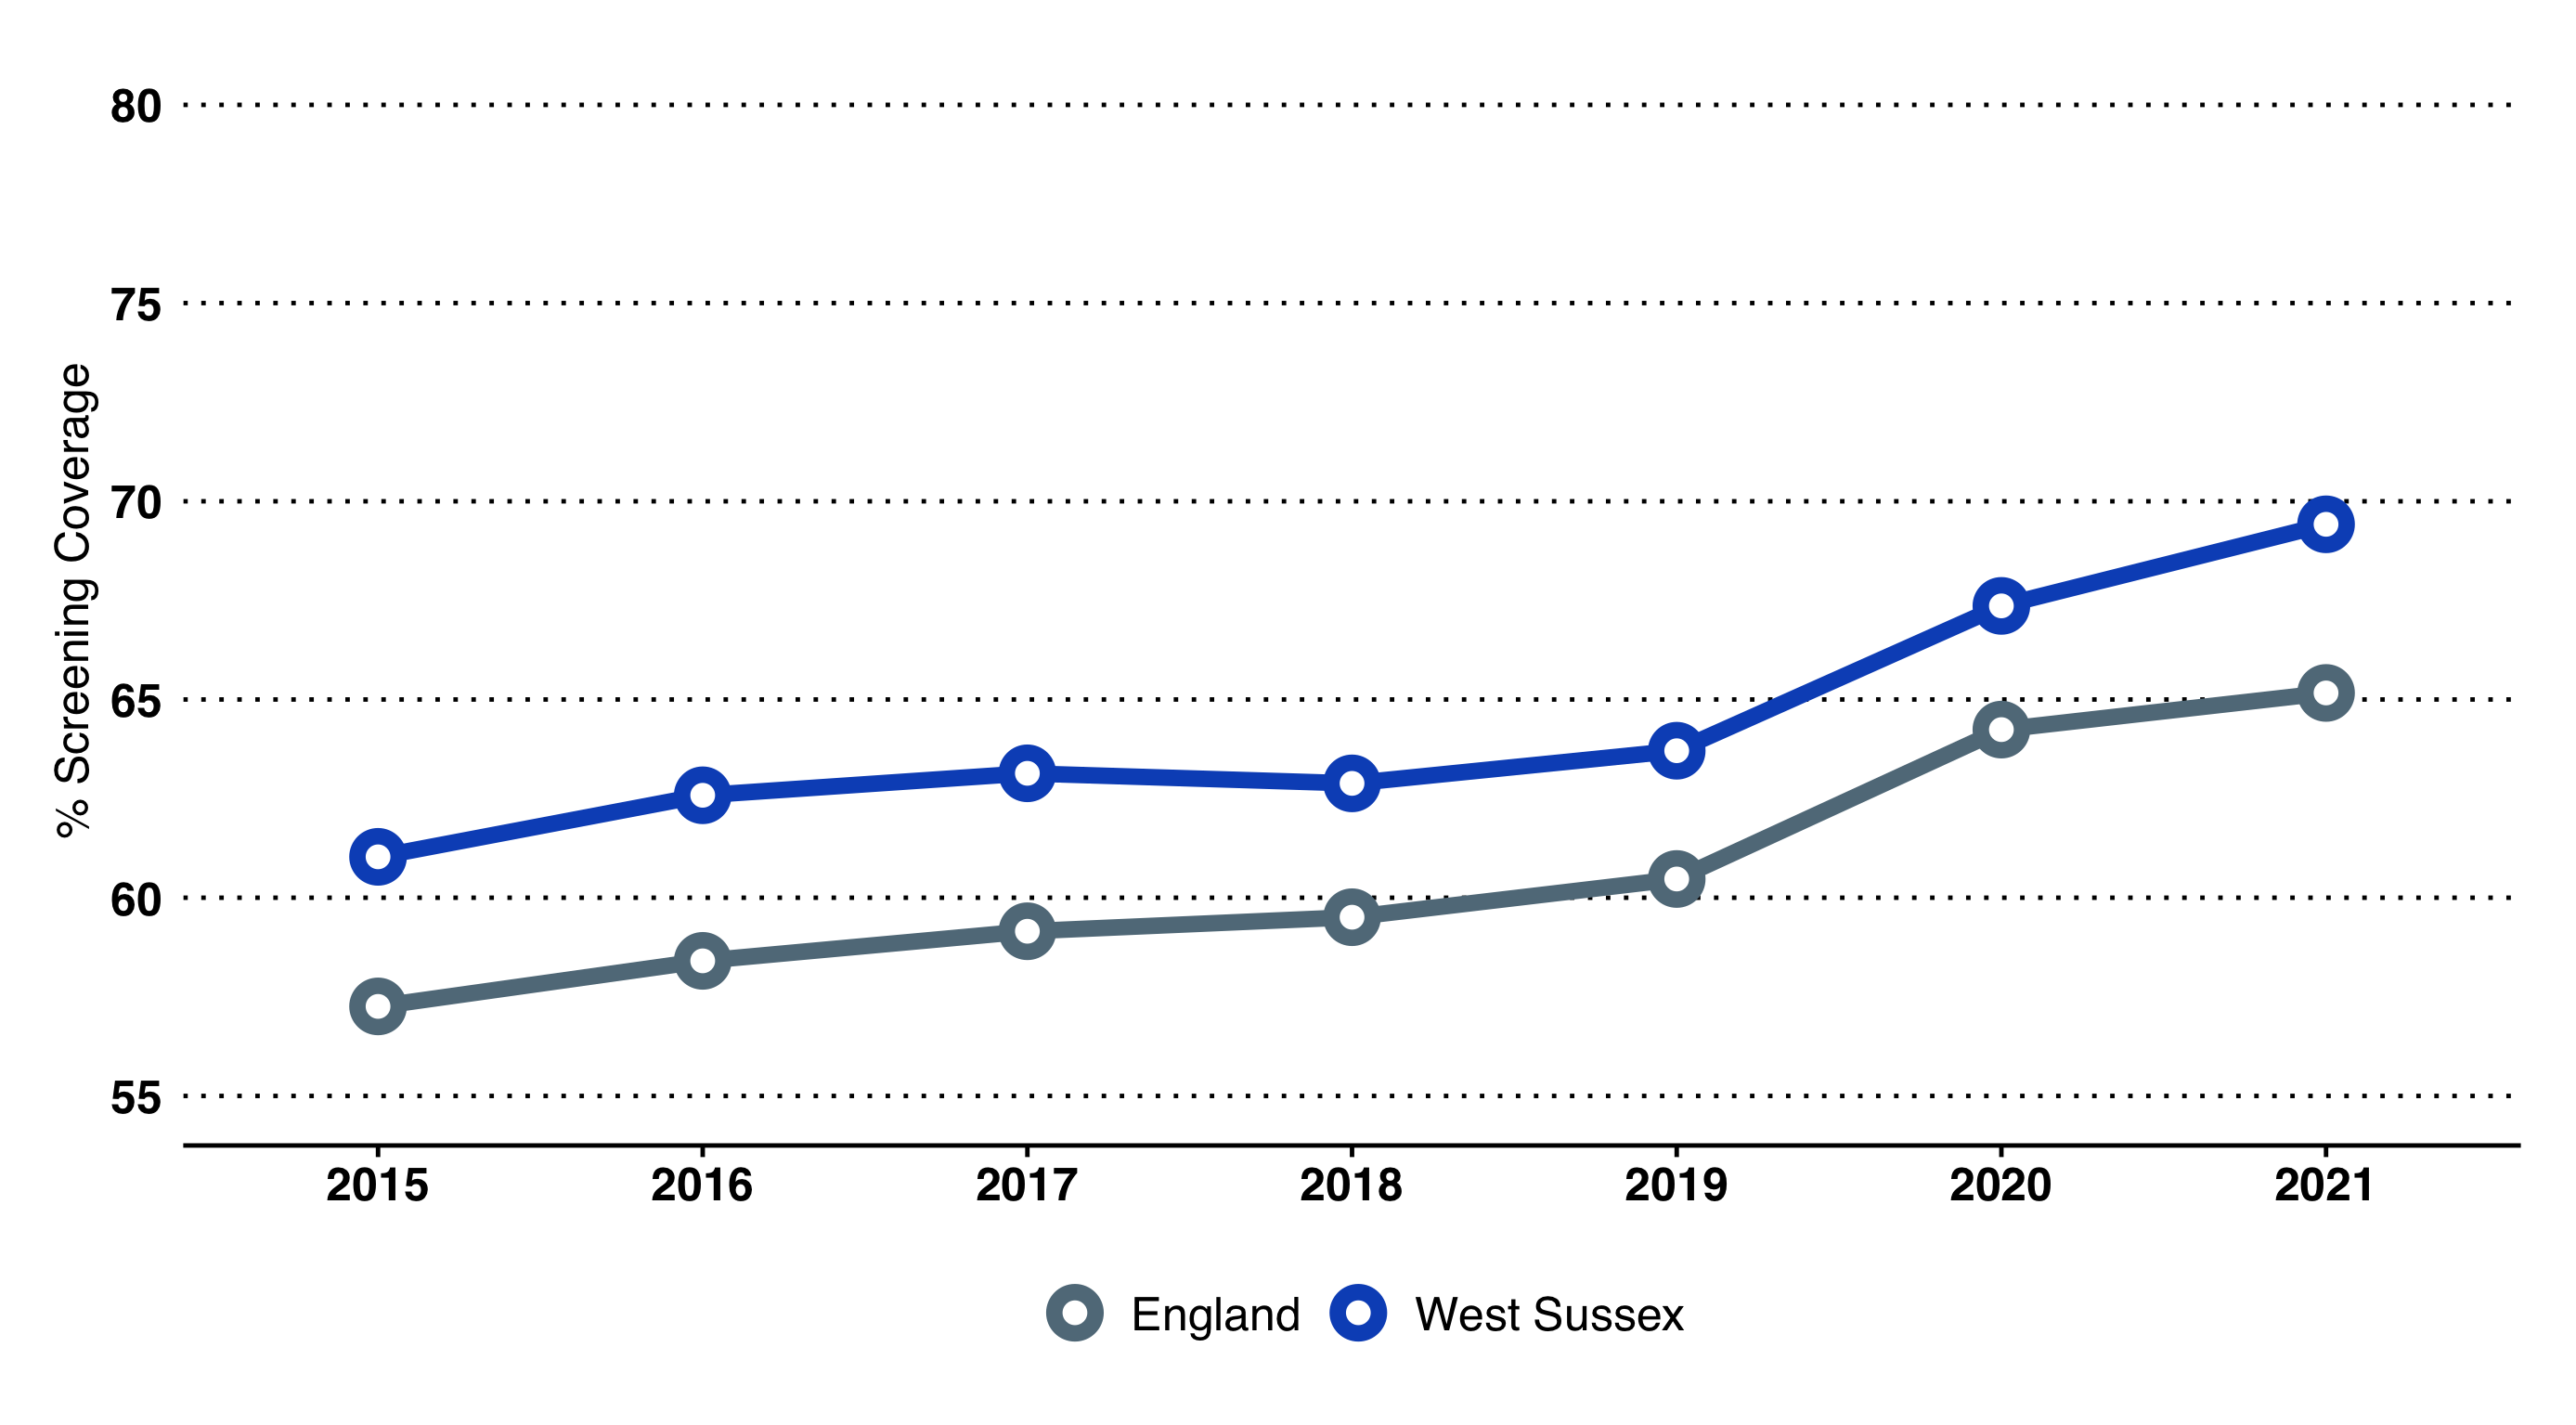
\includegraphics[width=\textwidth]{images/bowel_cancer_screening.png}
        \caption{Bowel Cancer screening coverage - West Sussex and England over time}
        \label{fig:bowel:time}
    \end{subfigure}
\end{figure*}

% Cervical - 

% \begin{figure}
%     \caption{Breast cancer screening coverage 2019/20 West Sussex Local Authorities}
%     \centering
%     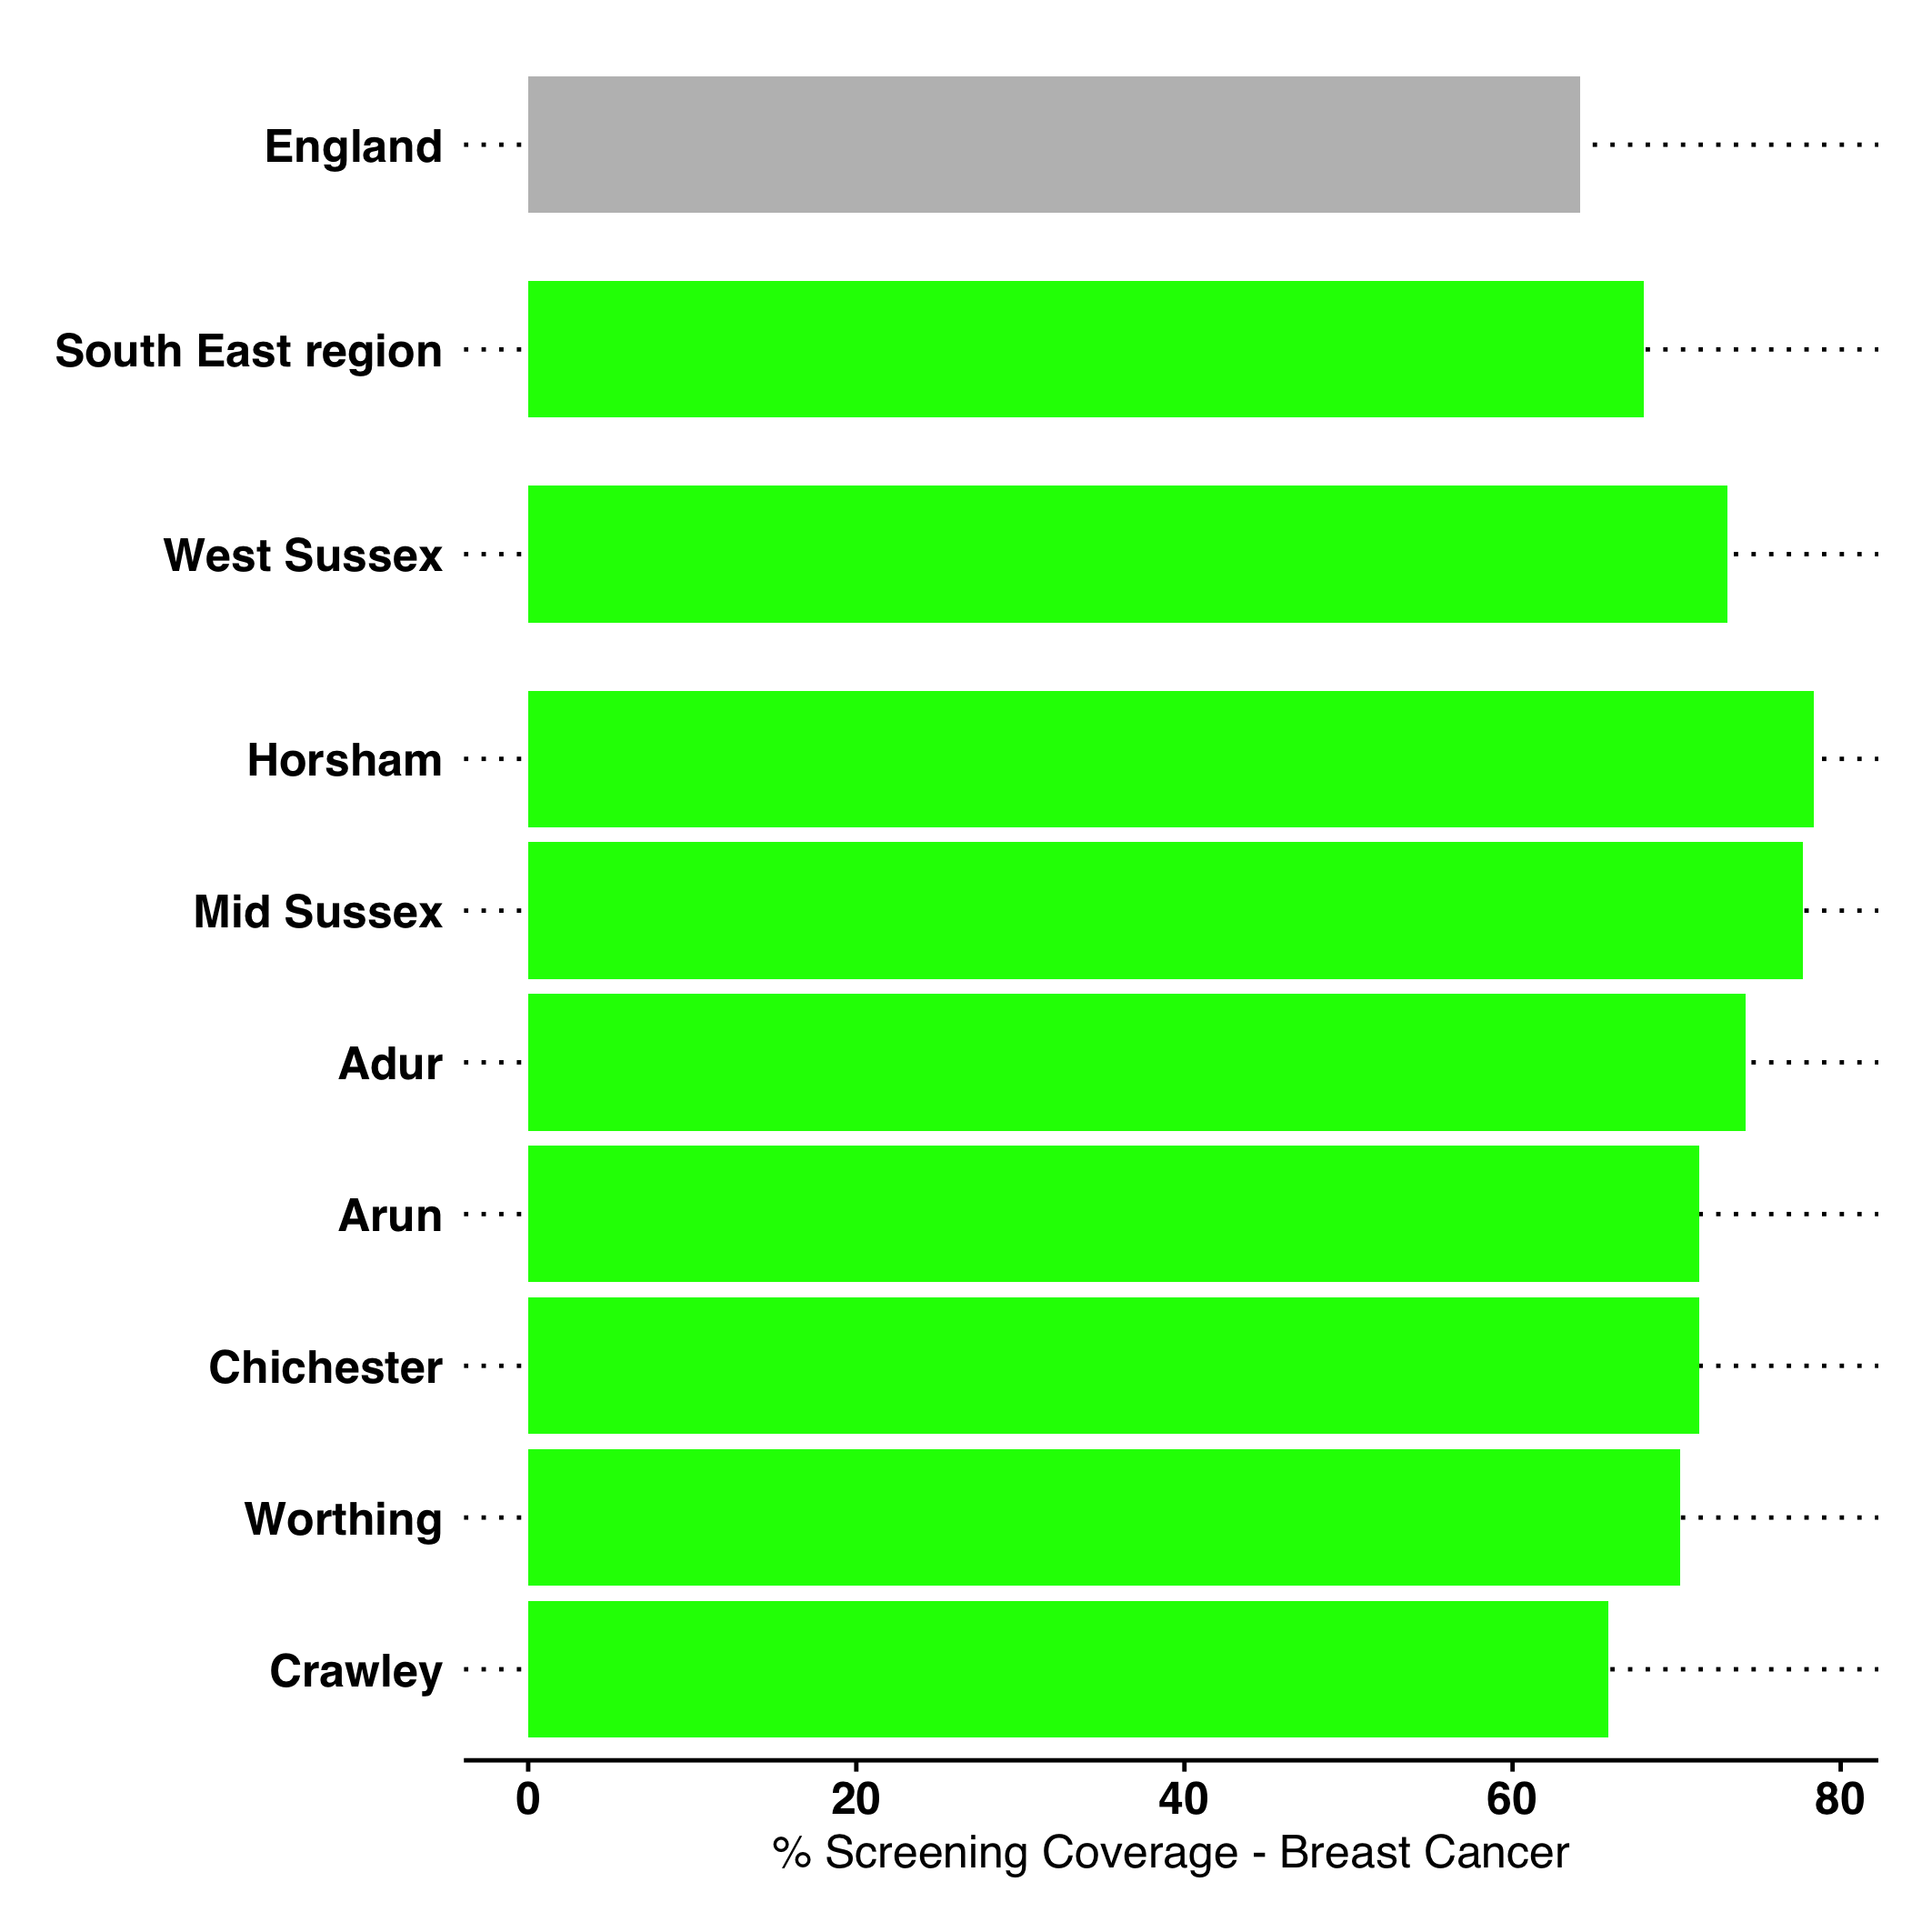
\includegraphics[width=\linewidth]{images/breast_cancer_rag_bar.png}
%     \label{fig:breast:rag}
% \end{figure}

% \begin{figure}
%     \caption{Breast Cancer screening coverage - West Sussex over time}
%     \centering
%     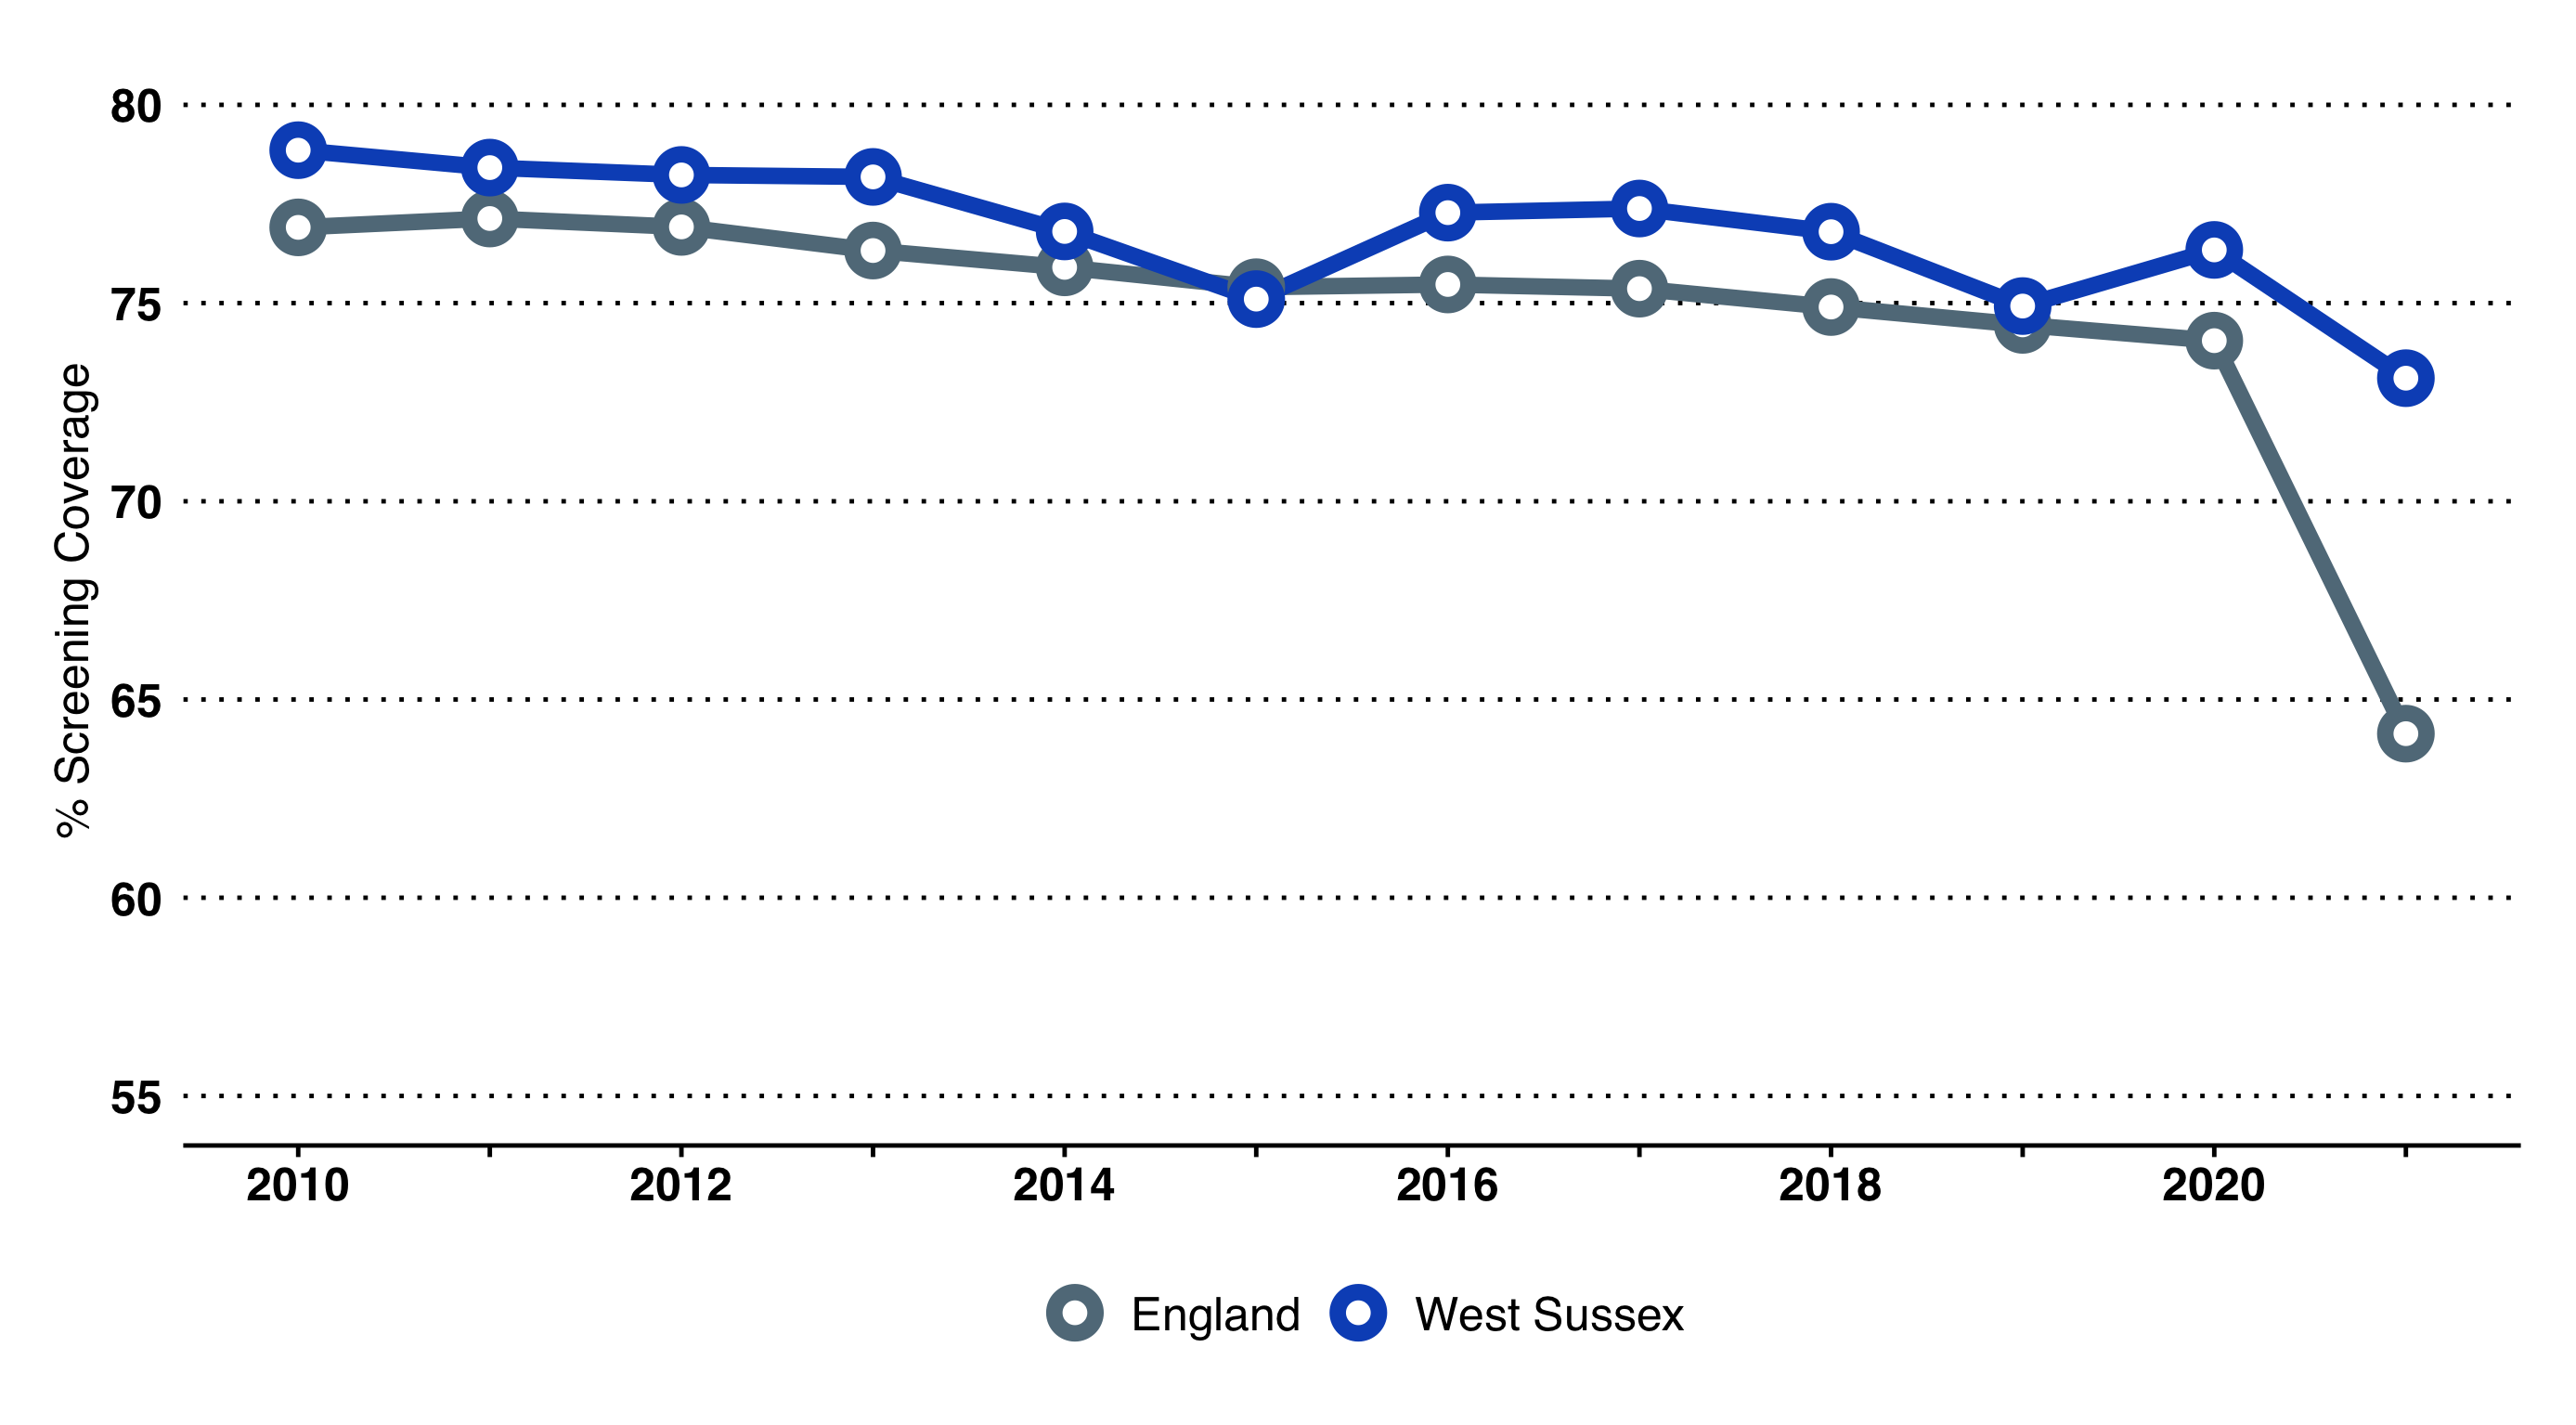
\includegraphics[width=\linewidth]{images/breast_cancer_screening.png}
%     \label{fig:breast:time}
% \end{figure}

% Breast - The screening rate at county-level for breast cancer is 74.9\% (Crawley, 70.3\%)(PHOF reference C24a). Recent issues with the West Sussex breast programme's round length may explain the decline in screening coverage.

% \begin{figure}
%     \caption{Bowel cancer screening coverage 2019/20 West Sussex Local Authorities}
%     \centering
%     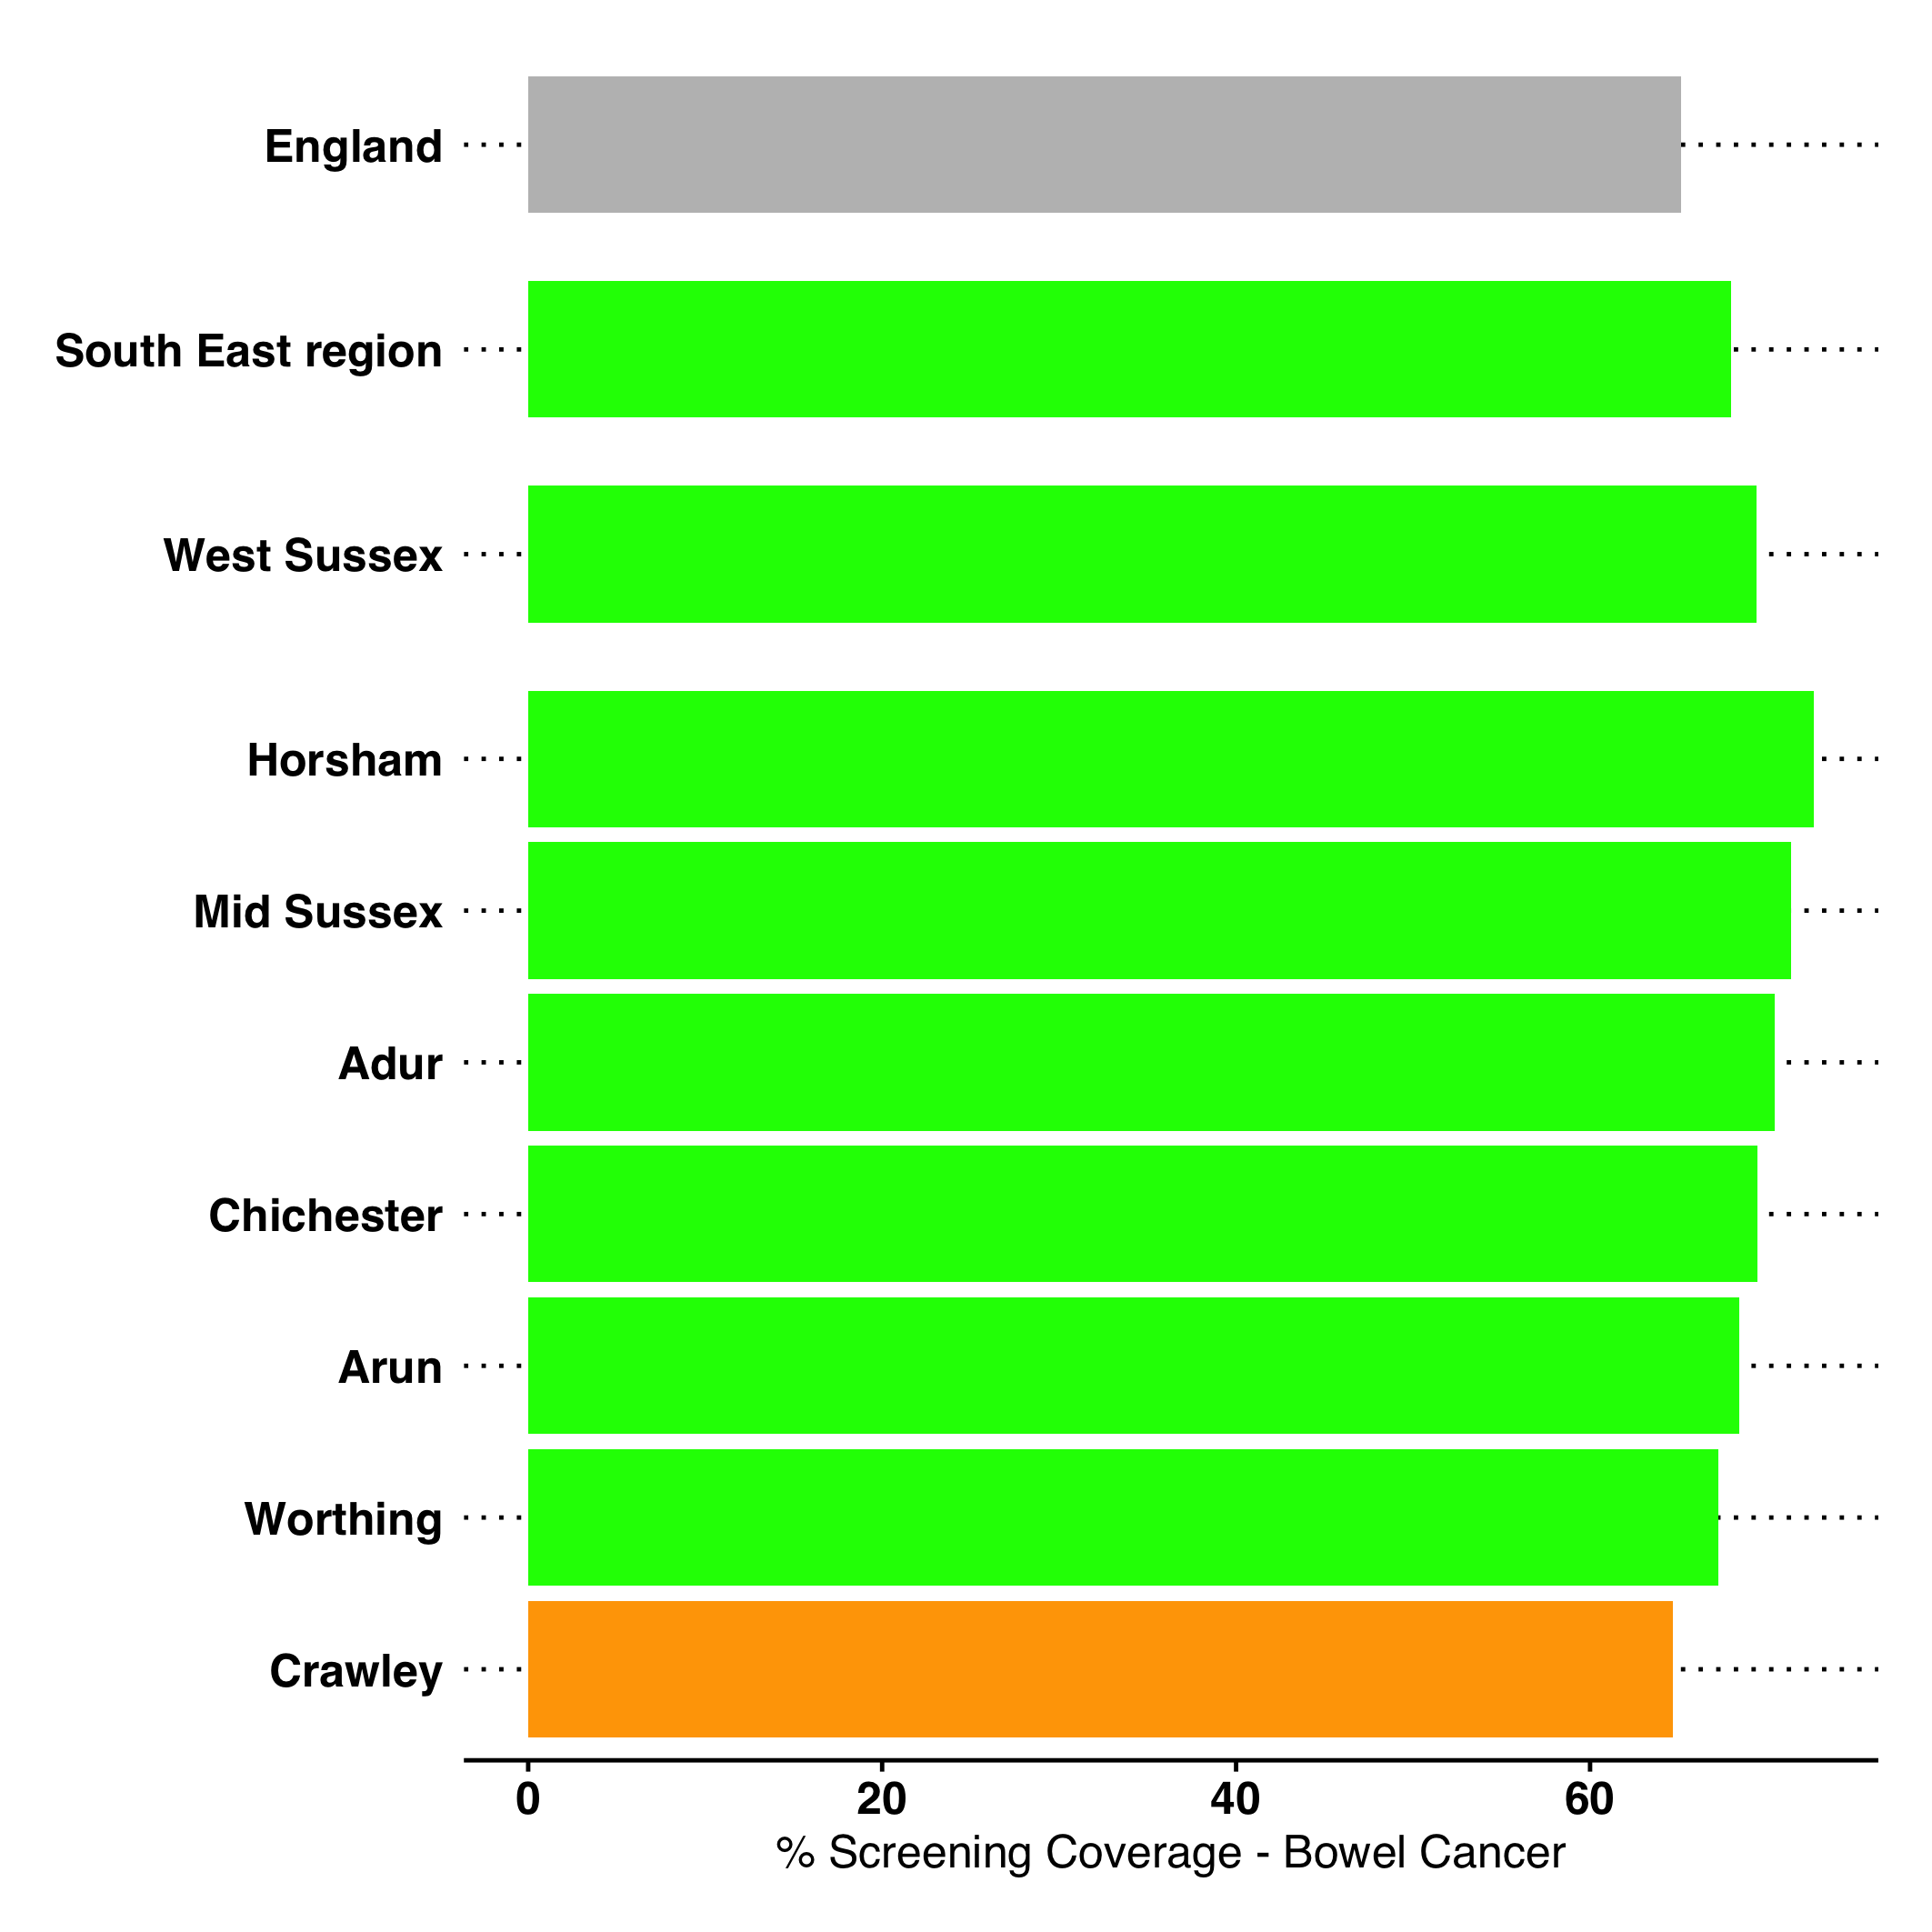
\includegraphics[width=\linewidth]{images/bowel_cancer_rag_bar.png}
%     \label{fig:bowel:rag}
% \end{figure}

% \begin{figure}
%     \caption{Bowel cancer screening coverage - West Sussex over time}
%     \centering
%     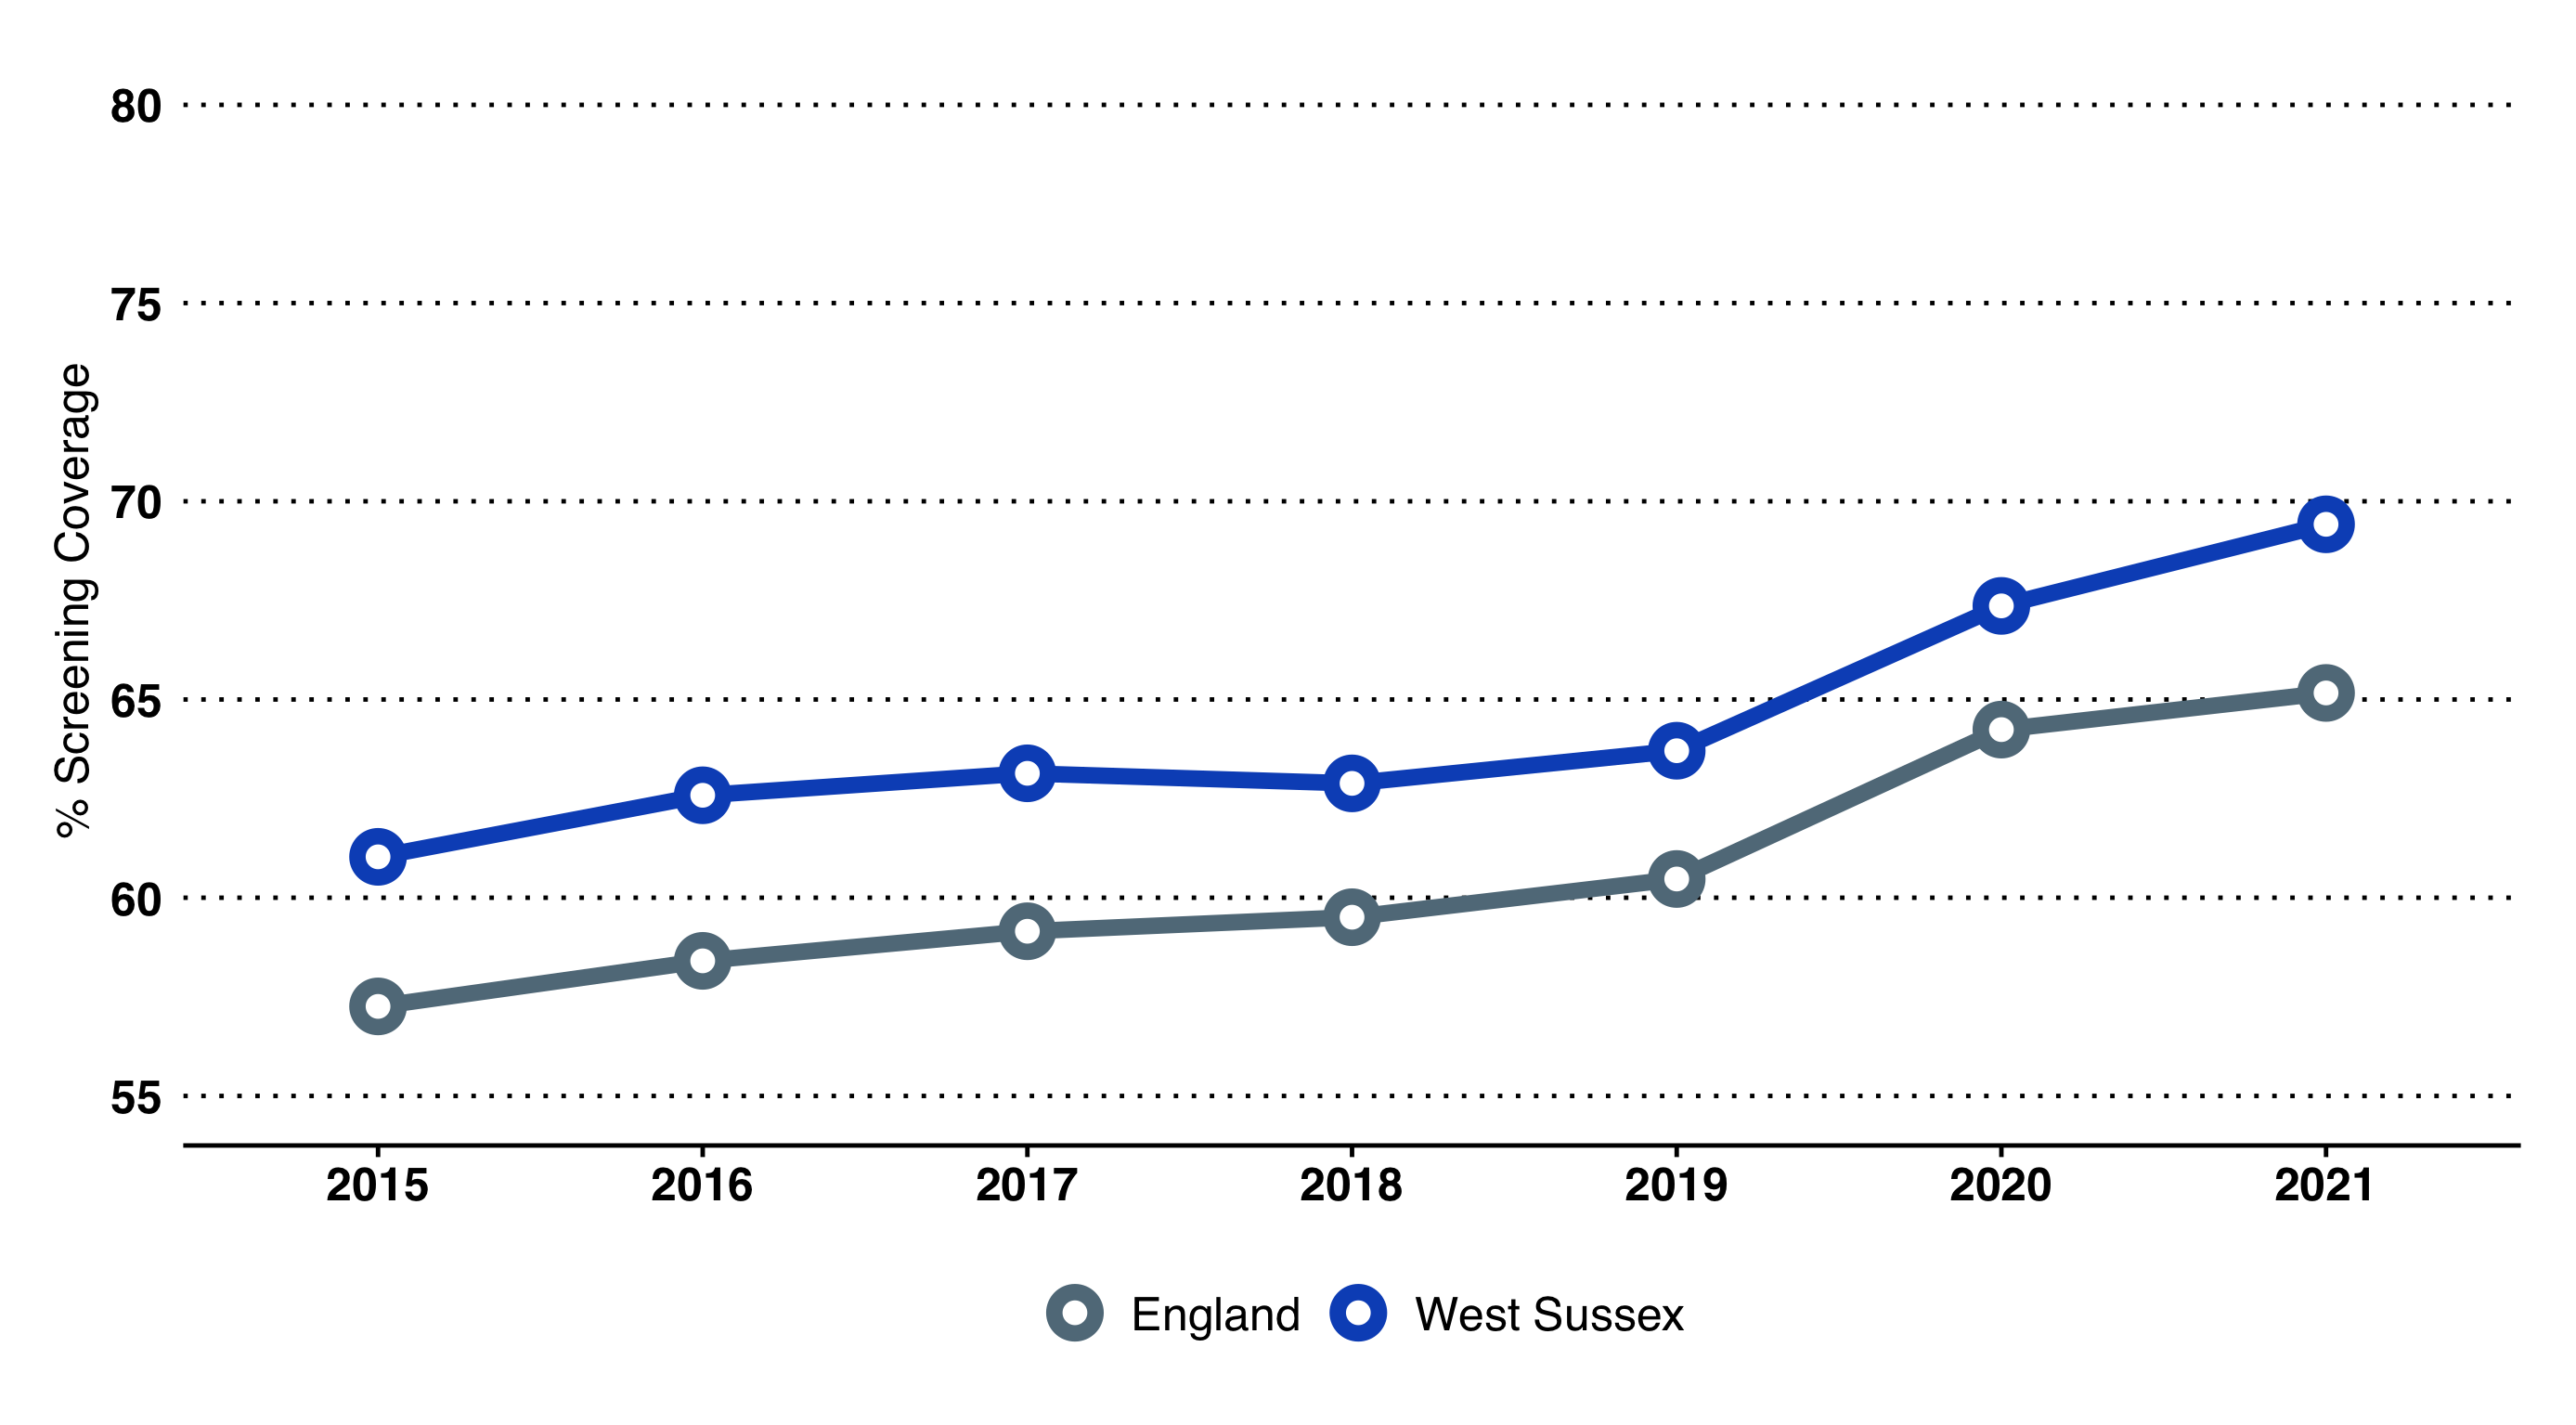
\includegraphics[width=\linewidth]{images/bowel_cancer_screening.png}
%     \label{fig:bowel:time}
% \end{figure}

% Bowel - 

\clearpage

\subsection{Mental Health}
Many of the prevalence assumptions for adult mental health conditions are derived from national surveys and research. Of particular note is the Adult Psychiatric Morbidity Survey (APMS). The APMS provides data on the prevalence of treated and untreated psychiatric disorders among adults (aged 16+) in households in England. The most recent survey was conducted in 2014 (McManus, Bebbington, Jenkins, \& Brugha, 2016) and is the fourth in the series (previous survey years include: 1993, 2000 and 2007).

\subsubsection{APMS Key Findings}
\begin{itemize}[noitemsep]
    \item Nationally, 1 in 6 adults (17.0\%) were identified with a common mental health disorder (CMD) in the week prior to being interviewed APMS. Applying this prevalence estimate to West Sussex, it is estimated that 121,200 adults (aged 16+) are likely to have a common mental health problem\footnote{Note that the national estimate is a synthetic estimate. Note also that a synthetic prevalence estimate of 14.4\% exists for West Susssex, which is equivalent to approximately 102,600 people based on current population estimates.}.
    \item Women were more likely to have a common mental health disorder than men.
    \item 64.4\% of adults who were identified as having a common mental health disorder in the survey had been diagnosed by a professional.
    \item Around a third (35.6\%) of adults identified as currently with CMD by the survey have never been diagnosed. This may reflect unmet need, or demonstrate how perceptions of mental health vary.
\end{itemize}

\begin{table*}
    \caption{Estimates of Prevalence of Common Mental Health Disorders in West Sussex by age group (Adult Psychiatric Morbidity Survey 2014, applied to West Sussex 2020 Population estimates)}
    \centering
    \begin{tabular}{lrrrrrrrr}
        \toprule
        \ & 16-24 & 25-34 & 35-44 & 45-54 & 55-64 & 65-74 & 75+ & All \\
        \midrule
        Generalised anxiety disorder & 4,530 & 5,670 & 7,370 & 8,870 & 7,510 & 4,140 & 2,470 & 42,050 \\
        Depressive episode & 1,660 & 3,250 & 4,380 & 5,470 & 5,040 & 2,170 & 1,280 & 23,520 \\
        Phobias & 2,380 & 3,070 & 3,210 & 3,280 & 2,700 & 620 & 490 & 17,100 \\
        Obsessive compulsive disorder & 1,300 & 1,300 & 1,710 & 1,940 & 1,760 & 310 & 300 & 9,260 \\
        Panic disorder & 860 & 460 & 320 & 610 & 590 & 720 & 590 & 4,280 \\
        CMD-NOS (not otherwise specified) & 6,050 & 8,460 & 8,760 & 10,570 & 9,500 & 5,380 & 4,830 & 55,590 \\
        Any CMD & 13,600 & 17,660 & 20,620 & 23,200 & 21,110 & 11,900 & 8,680 & 121,160 \\
        \bottomrule
    \end{tabular}
    \label{tab:wa:cmd}
\end{table*}


 
\subsubsection{Severe Mental Illness} The mental health register is a count of the total number of people with schizophrenia, bipolar disorder and other psychoses. In 2020/21, the recorded disease prevalence for mental health was 0.91\% in West Sussex CCG, which is lower than that of England as a whole (0.95\%).

\begin{table}
    \caption{Recorded disease prevalence for mental health conditions (schizophrenia, bipolar disorder and psychoses) (2016/17)}
    \centering
    \begin{tabular}{lrrr}
        \toprule
        \ & List Size & Register & Prevalence (\%) \\
        \midrule
        West Sussex CCG & 913,467 & 8,314 & 0.91 (CI: 0.88-0.94) \\
        England & 60,444,947 & 574,227 & 0.95 (CI: 0.94-0.95) \\
        \bottomrule
    \end{tabular}
    \label{tab:wa:mhc}
\end{table}

\subsubsection{Learning Disability} There are an estimated 17,200 people aged 15+ years living with a learning disability in West Sussex

\begin{itemize}
    \item 4,100 people with a moderate to severe learning disability
    \item 5,100 people on GP practice Learning disability registers
    \item 300 people with Down's syndrome
\end{itemize}

\paragraph{Autism} In relation to adults (18+ years) it is estimated that there are 1,100 adults in West Sussex living with autism.

\subsubsection{Wellbeing}
People with higher wellbeing have lower rates of illness, recover more quickly and for longer, and generally have better physical and mental health. As a key health issue, ONS has developed new measures to estimate national wellbeing. Four questions included in the Integrated Household Survey are used to measure individual (and therefore subjective) wellbeing. These ask, on a scale of 0-10, overall:

\begin{itemize}[noitemsep]
    \item how satisfied are you with your life nowadays?
    \item how happy did you feel yesterday?
    \item how anxious did you feel yesterday?
    \item to what extent do you feel the things you do in your life are worthwhile?
\end{itemize}

{\bf Note}: these measures are estimates, based on a sample of the population from each area. Some years may lack data due to too small sample sizes or have wide confidence intervals (i.e. the range in which the true estimate could lie).

\paragraph{People with a low satisfaction score} 4.2\% of people gave a low life satisfaction score\footnote{PHOF reference C28a} (those scoring 0-4/10; confidence intervals 2.8-5.6\%) in 2017/18, similar to the England score in this period (4.4\%).

\paragraph{People with a low worthwhile score} 3.5\% of people gave a low worthwhile score\footnote{PHOF reference C28b} (those scoring 0-6/10; confidence intervals 2.1-4.8\%) in 2017/18, similar to the England score (3.6\%) in this period. Trend data is not available for this measure, as the sample size of the most recent and previous years is too small.

\paragraph{People with a high anxiety score} 17.6\% of people gave a high anxiety score\footnote{PHOF reference C28d} (those scoring 6-10/10; confidence intervals 14.7-20.5\%) in 2018/19. This is lower than the England score (19.7\%) and the fourth lowest score amongst CIPFA neighbours.

\paragraph{People with a low happiness score} 6.8\% of people gave a low life happiness score\footnote{PHOF reference C28c} (those scoring 0-4/10) in 2018/19. This is slightly lower than the England score (7.8\%), although not significantly different (confidence intervals 4.8-8.8\%) and of middling position compared to CIPFA neighbours.

\begin{figure*}
    % At county-level, overall take-up rates of screening programmes are good, comparing favourably with England and in line with rates in statistical neighbours. However, there is variation between the West Sussex local authorities, with notably low rates in Crawley. All relate to 2020/21.\\
    \caption[Measurement of wellbeing in the Integrated Household Survey.]{Measurement of wellbeing in the Integrated Household Survey.}\label{fig:wellb-survey}
    \vspace*{3mm}
    \centering
    \begin{subfigure}[b]{0.48\textwidth}
        \centering
        \caption{People with a low satisfaction score}\label{fig:wellb-surv:satis}
        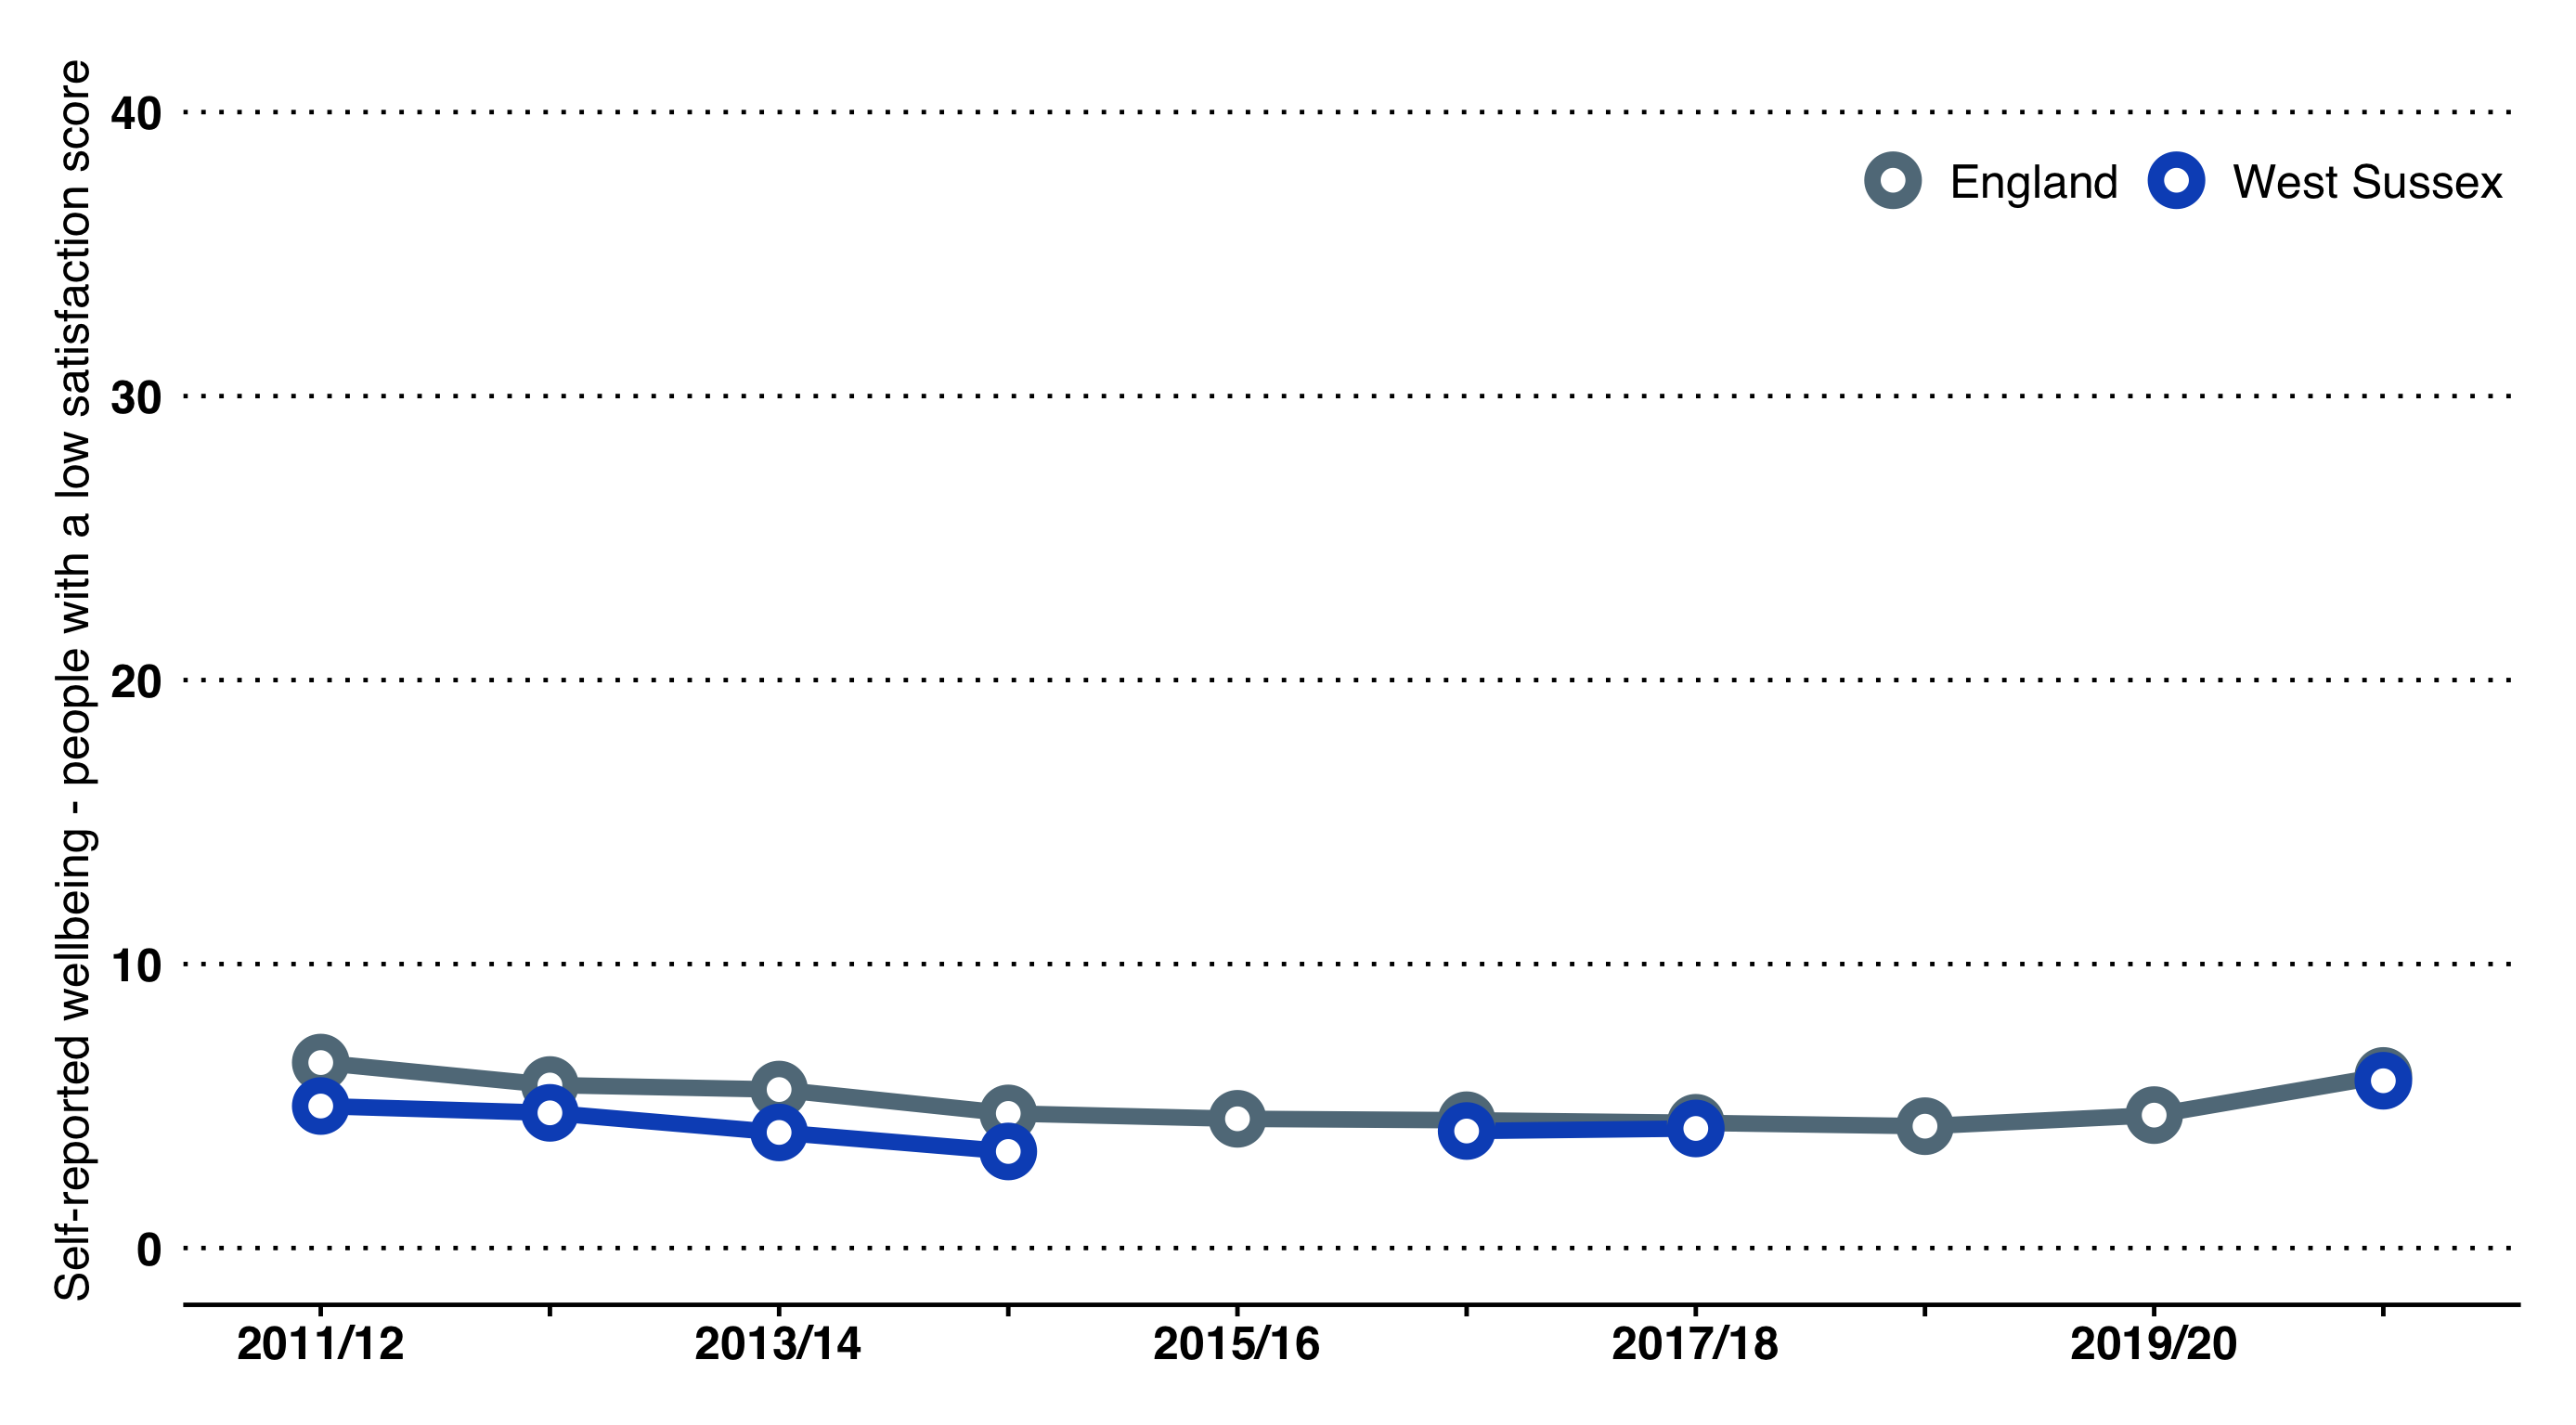
\includegraphics[width=\textwidth]{images/low_satisfaction_line.png}
    \end{subfigure}
    \begin{subfigure}[b]{0.48\textwidth}
        \centering
        \caption{People with a low worthwhile score}\label{fig:wellb-surv:loww}
        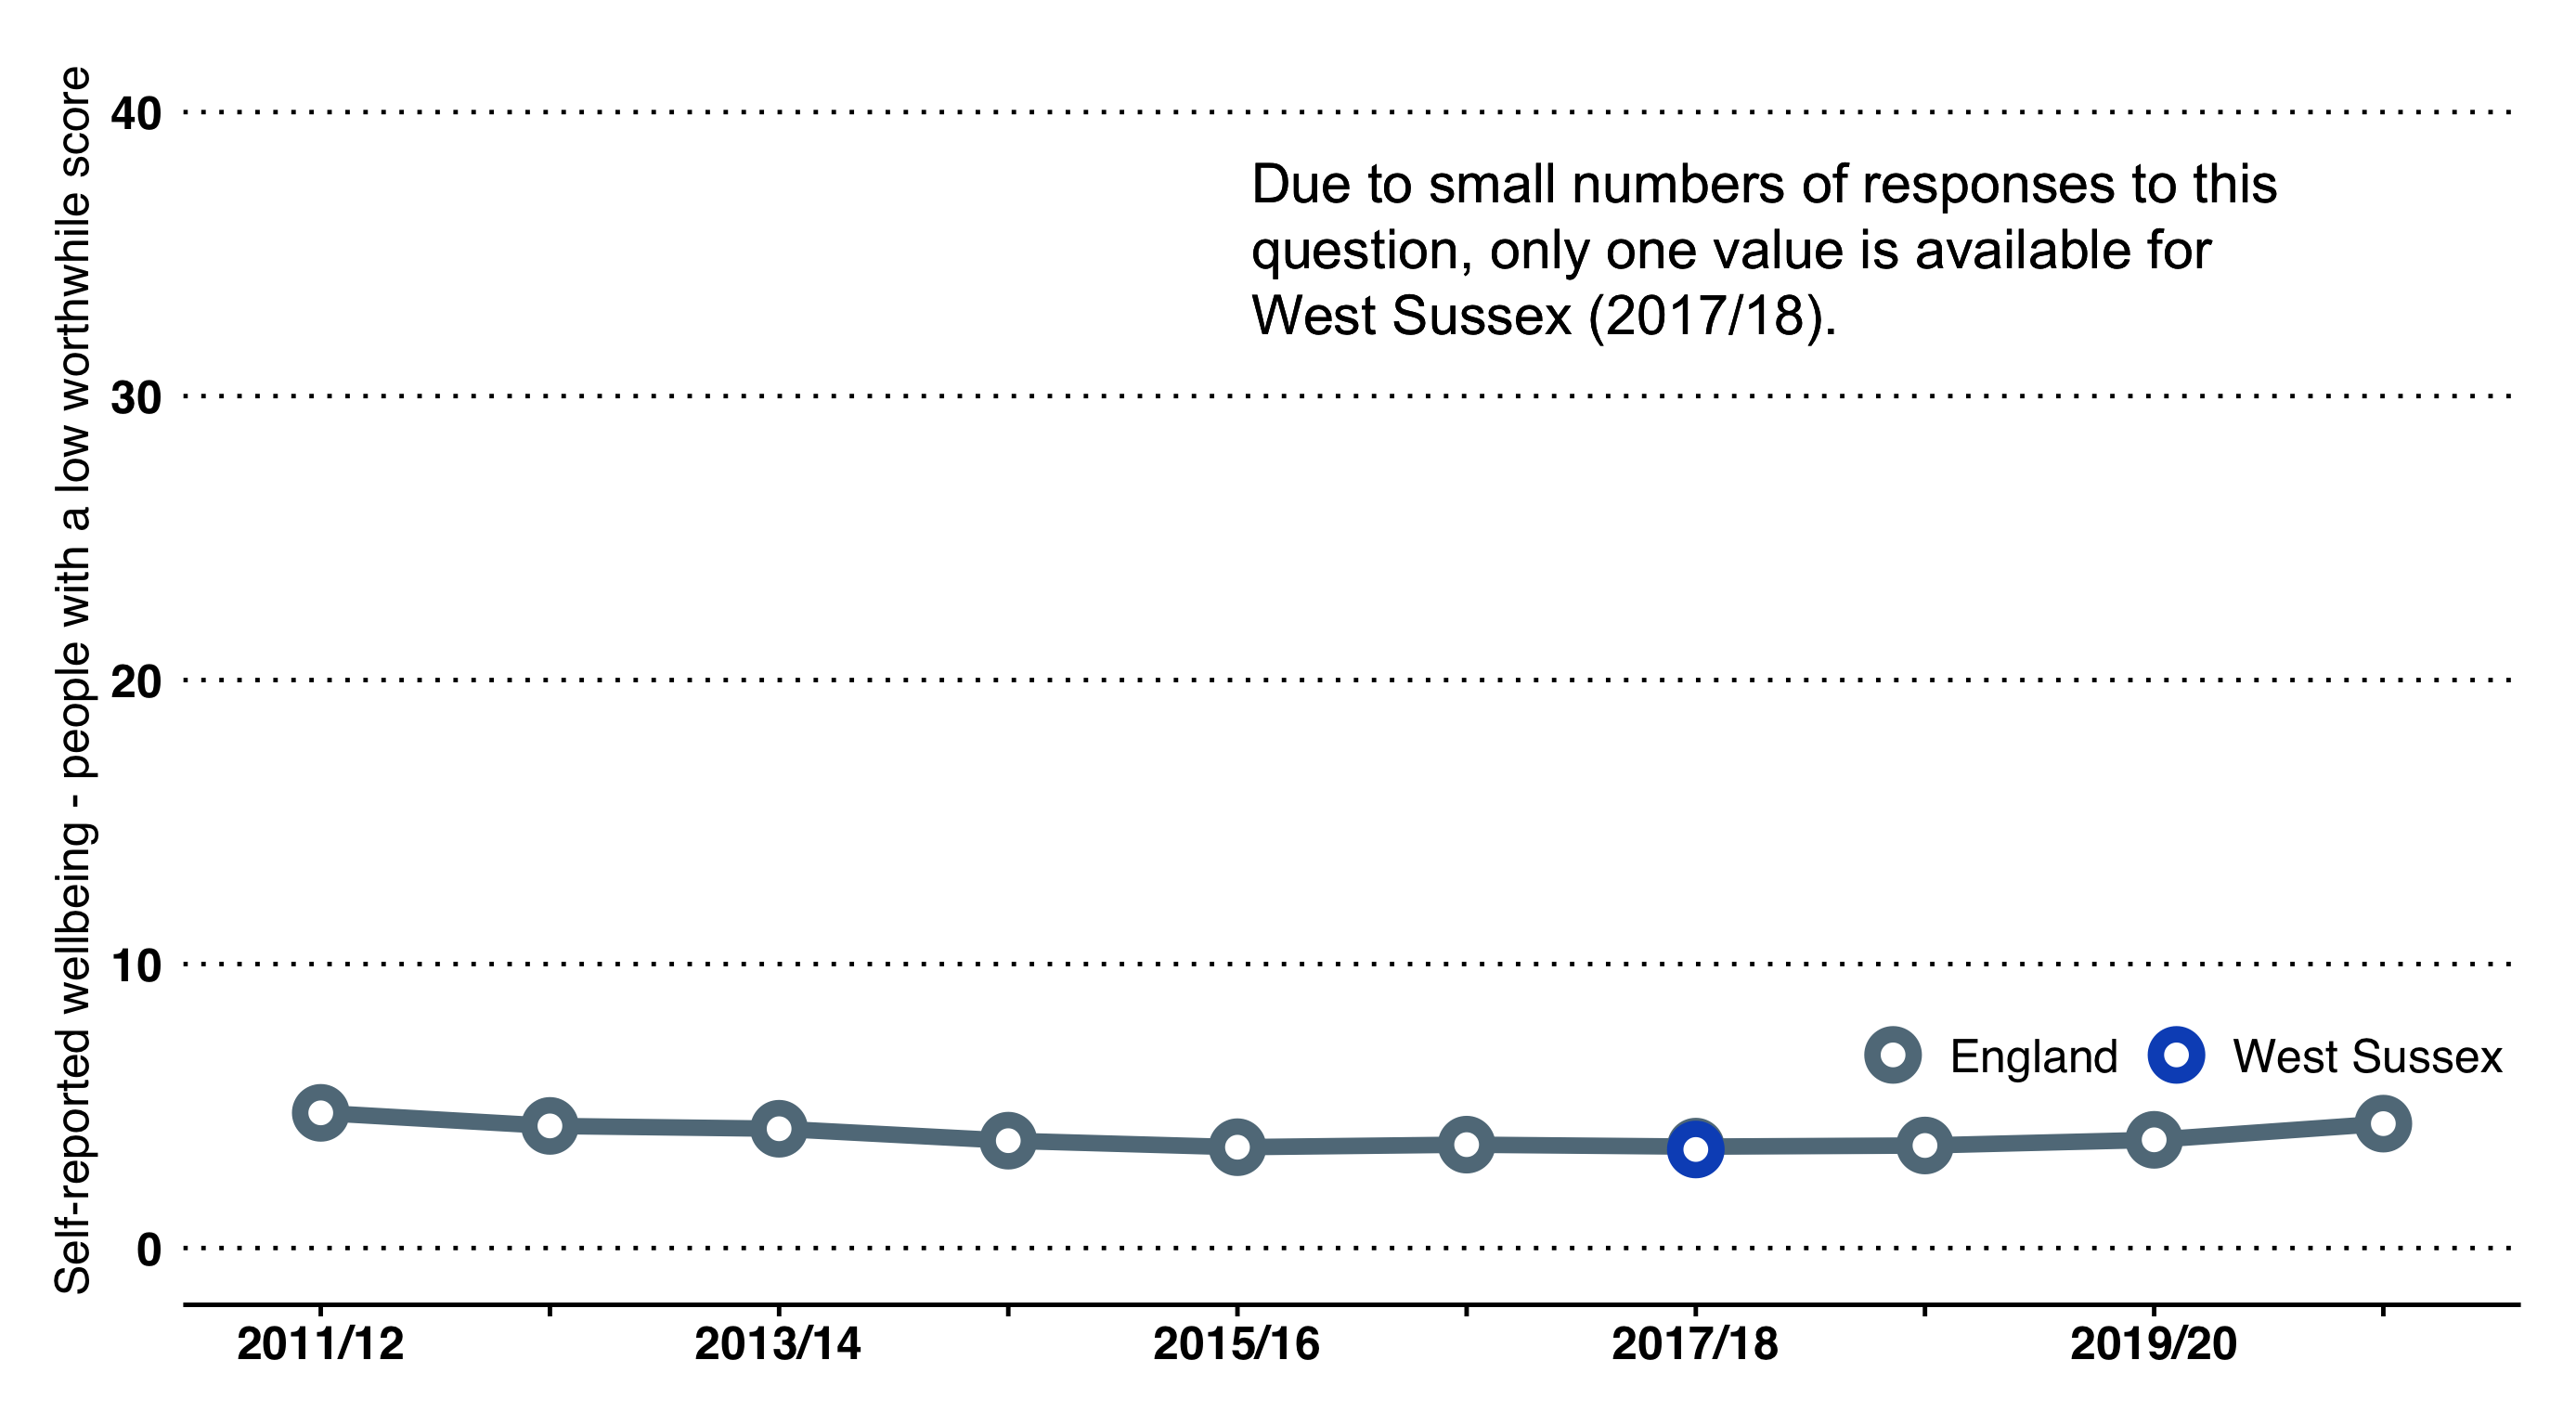
\includegraphics[width=\textwidth]{images/low_worthwhile_line.png}
    \end{subfigure}
    \vspace*{3mm}
    \begin{subfigure}[t]{0.48\textwidth}
        \centering
        \caption{People with a high anxiety score}\label{fig:wellb-surv:hanx}
        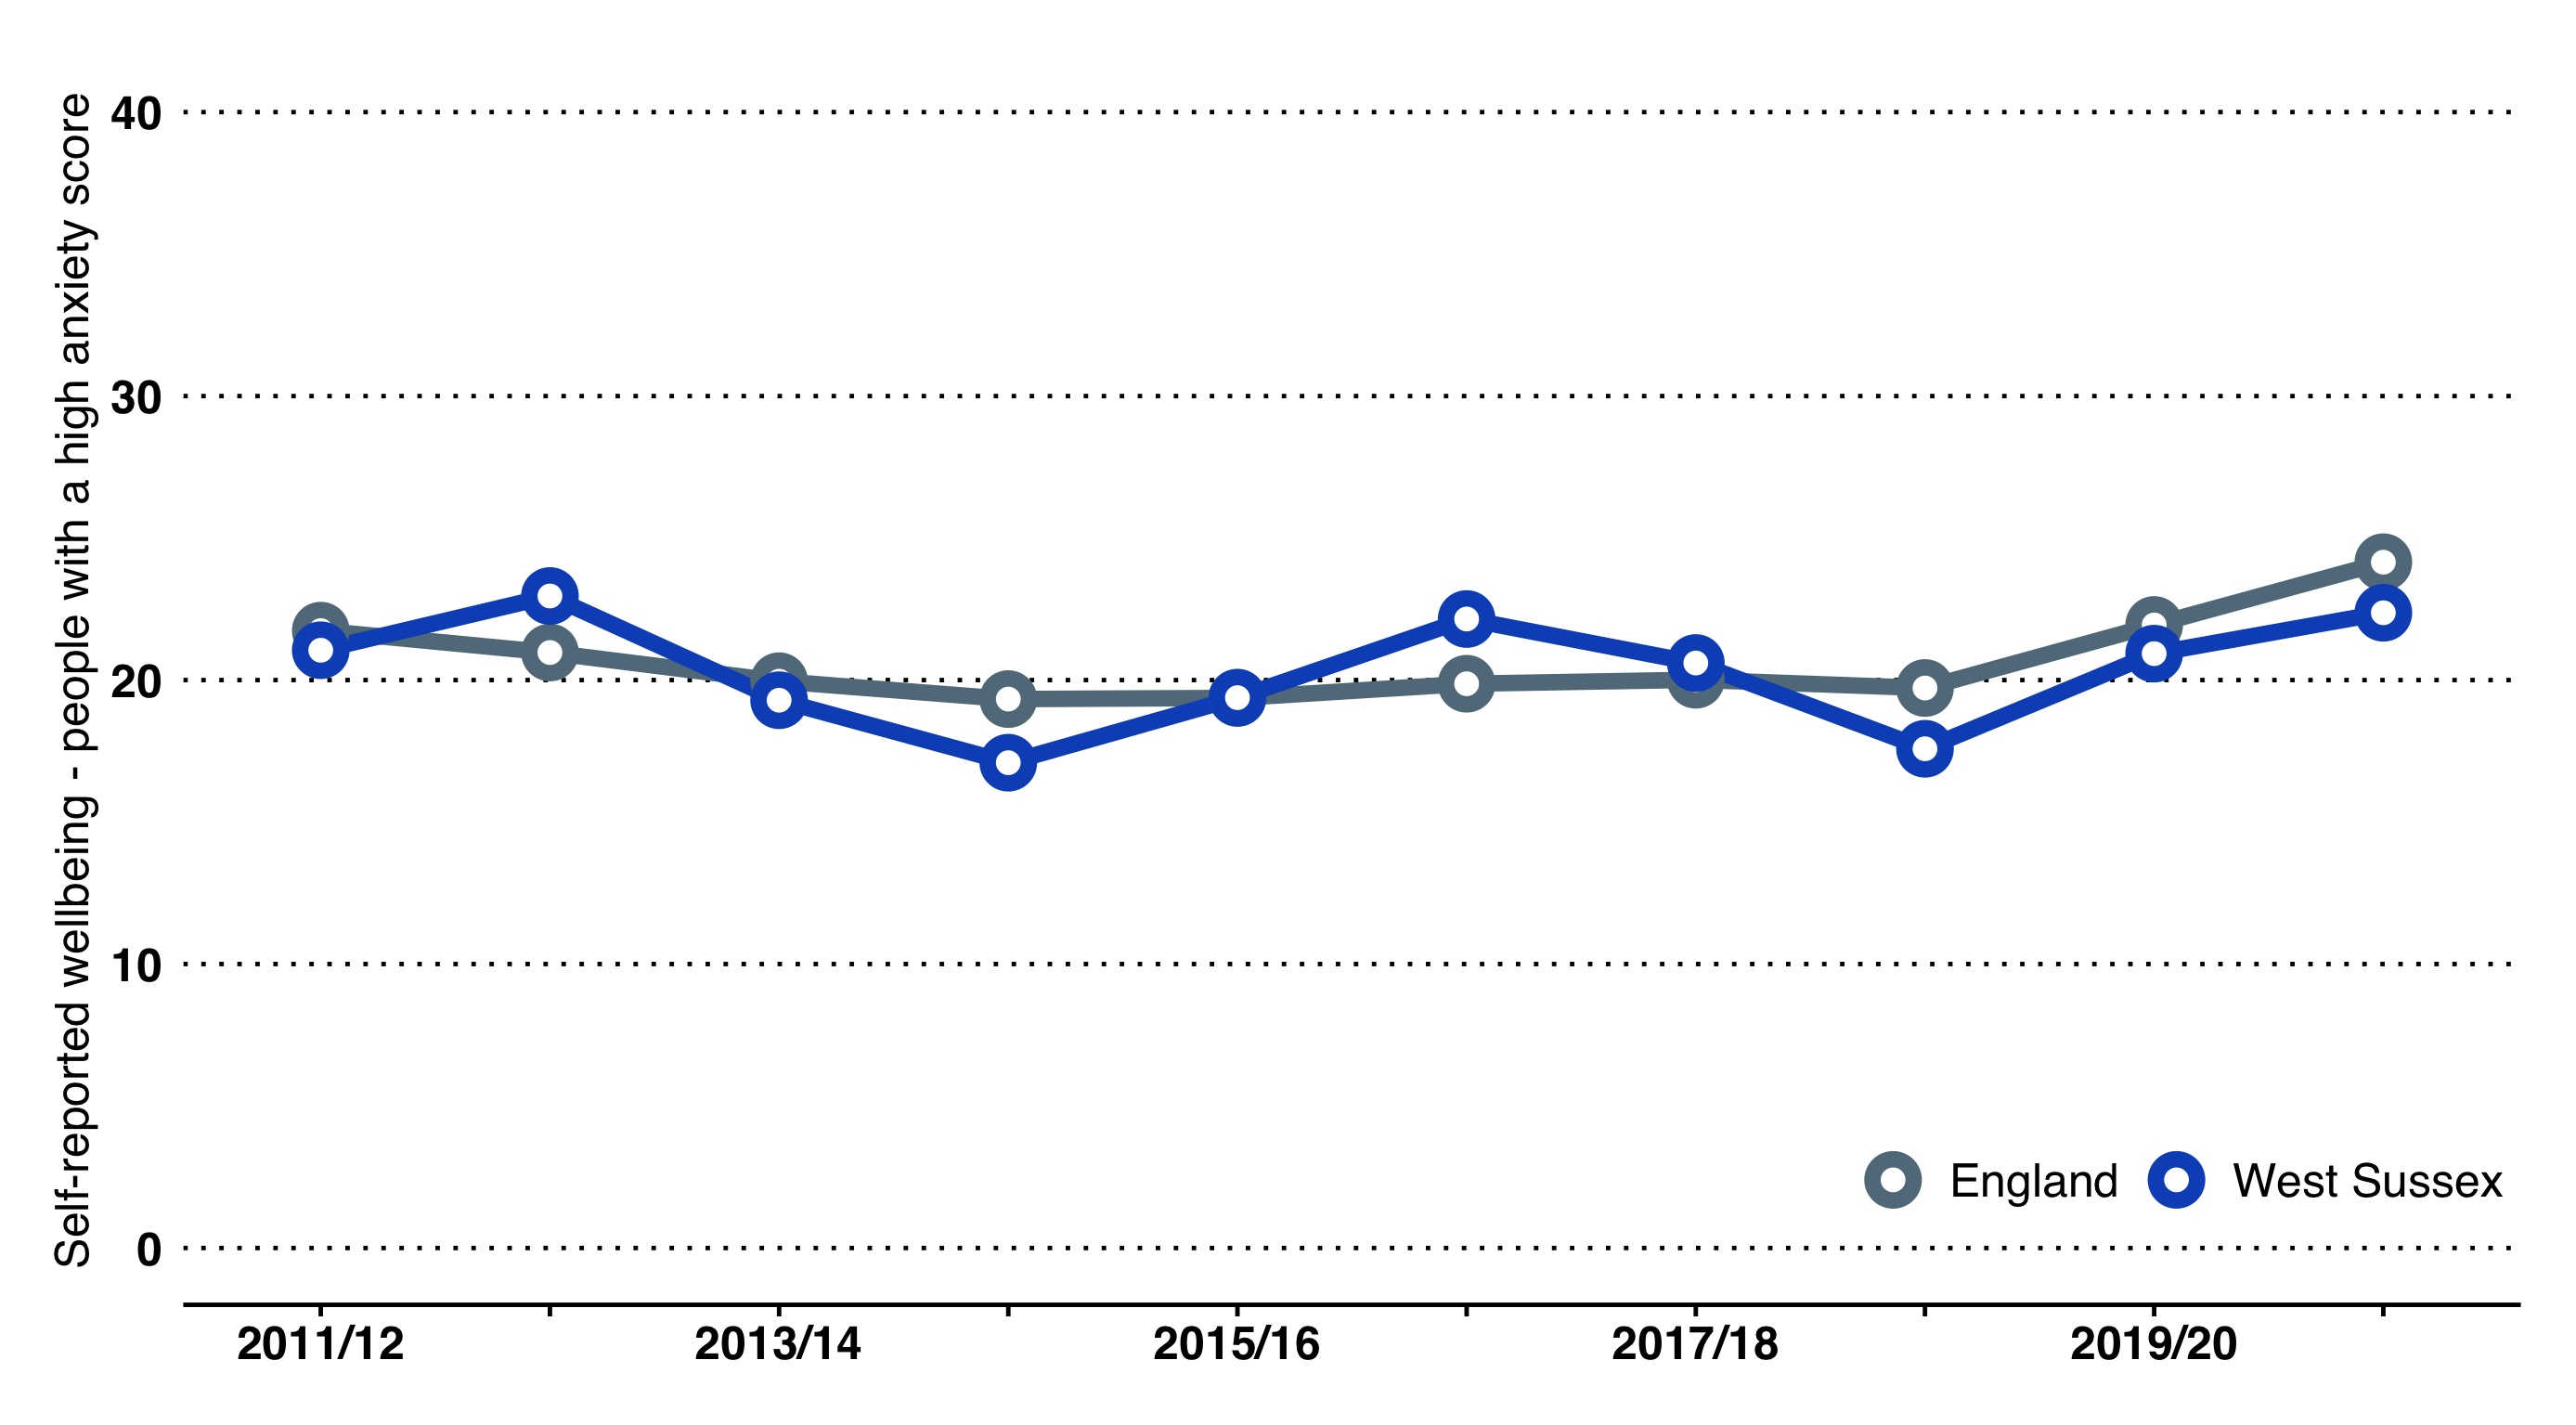
\includegraphics[width=\textwidth]{images/high_anxiety_line.png}
    \end{subfigure}
    \begin{subfigure}[t]{0.48\textwidth}
        \centering
        \caption{People with a low happiness score}\label{fig:wellb-surv:lhap}
        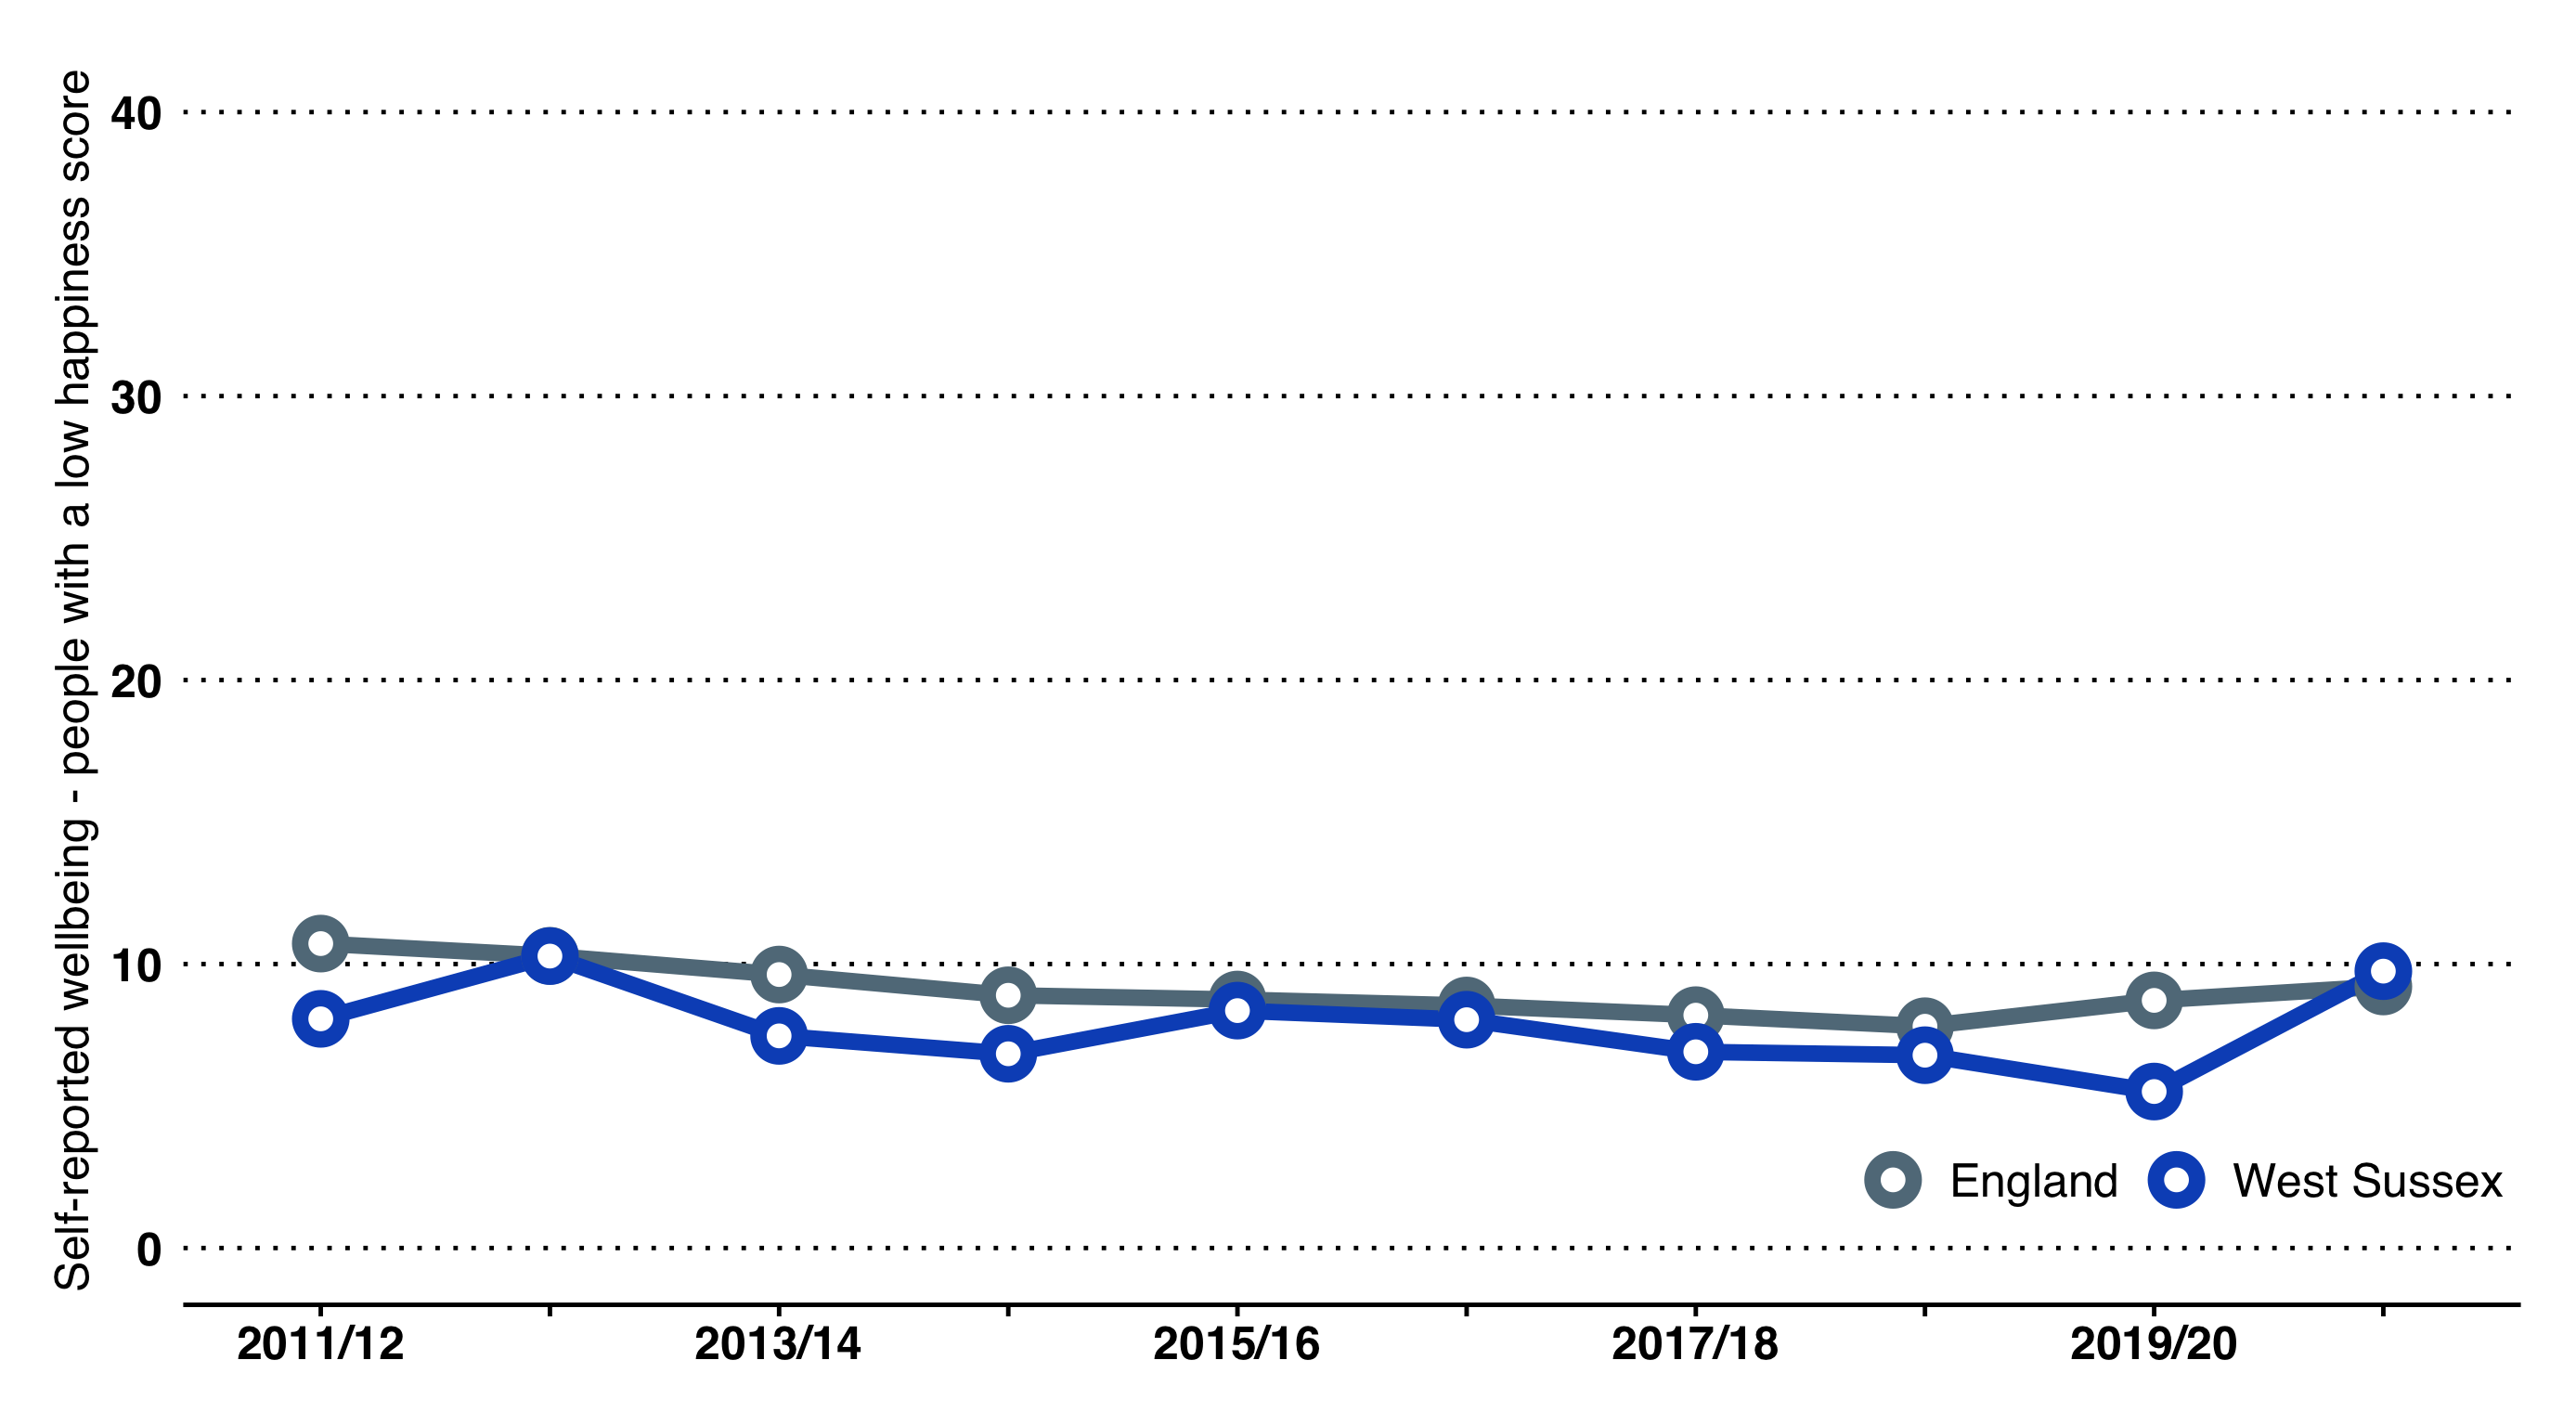
\includegraphics[width=\textwidth]{images/low_happiness_line.png}
    \end{subfigure}
\end{figure*}

\clearpage

\subsubsection{Measuring Wellbeing}
There is not a single measure of health, wellbeing or happiness: different tools focus on different things. Six commonly used tools/instruments are summarised on this page.

\begin{itemize}[noitemsep]
    \item Some tools concentrate on one domain/theme, such as health-related quality of life (HRQ0L) e.g. the EQ-5D tool.
    \item Some look at subjective wellbeing (SWB), such as the ONS Wellbeing survey.
    \item Others consider what outcomes different policy-makers are seeking answers to, such as the ability of people to undertake personal care tasks or the ability to manage a condition (e.g. self-efficacy in the Patient Activation Measure, or undertaking daily activities in adult social care surveys).
    \item Some questions focus on the frequency a feeling/experience occurs, whilst others ask about intensity (e.g. WEMWBS asks about frequency whilst ONS Wellbeing asks about intensity).
\end{itemize}

% To improve the understanding of tools available we have drafted a briefing of the main options available, which is available on the JSNA website.
% For further information please contact Clare Toon (\url{clare.toon@westsussex.gov.uk}) or Jacqueline Clay (\url{jacqueline.clay@westsussex.gov.uk}).

\begin{tcolorbox}[colback={boxcolour}, title={ONS Subjective Wellbeing}]
    Subjective wellbeing, designed as an adjunct to GDP measurement at a national level. Questions include evaluation, eudemonic and experience approaches.
    
    {\bf Pros:} Short, used widely. Nationally developed measure can be applied across programmes.
    
    {\bf Cons:} Not specifically centred on health, but broader subjective wellbeing. May not be sensitive to short term change
\end{tcolorbox}

\begin{tcolorbox}[colback={boxcolour},title={WEMWBS / Warwick Edinburgh}]
    Warwick Edinburgh Mental Wellbeing Measure, focuses on mental health and wellbeing and has a long and short version.

    {\bf Pros:} Widely used, long and short versions. Sums to provide a composite score, which can be useful in dissemination.

    {\bf Cons:} Centred on individual, using only positive statements. Scale relatively short, may not pick up small movement. In a recent local evaluation there were some problems reported in using with the very elderly (85+ years).
\end{tcolorbox}

\begin{tcolorbox}[colback={boxcolour},title={Outcomes Stars (wide range)}]
    Concentrates on using a specific format (spider diagram) and a wide range of measures for different groups and contexts within the population (e.g. young people, family, carers, homelessness)

    {\bf Pros:} Wide range of tools may be more suitable for specific conditions and circumstances, although less suitable for overall strategic reporting. Good visual format, easy to undertake

    {\bf Cons:} To use this tool an annual fee is paid (not prohibitive approx. £350)
\end{tcolorbox}

\begin{tcolorbox}[colback={boxcolour},title={Patient Activation Measure (PAM)}]
    Self-efficacy, willingness and ability to take on role of managing own health and health conditions. Describes activation in 4 levels (low activation to having the skills to self-manage)

    {\bf Pros:} Measures the ability of self-efficacy; the value is in understanding a patient's ability and starting point. Can be used across programmes.

    {\bf Cons:} Does not focus on issues of wider wellbeing. Fluctuates with deterioration, not necessarily linear assumption and not designed to be a high level performance measure. Costs (but not prohibitive)
\end{tcolorbox}

\begin{tcolorbox}[colback={boxcolour},title={EQ-5D}]
    Developed by the EuroQol Group as a measure of health-related quality of life. Widely used, has some overlap with ASCOF. Measure of intensity. Has a 3 level range version and a 5 level version
    
    {\bf Pros:} Widely used in health, wide application possible Easy, simple questions. Used for economic evaluation
    
    {\bf Cons:} Narrow view of health-related quality of life does not cover more subjective aspects of wellbeing. Requires registration but cost minimal.
\end{tcolorbox}

\begin{tcolorbox}[colback={boxcolour},title={ASCOF}]
    Measures social-care related quality of life - developed to assess whether a person's social care needs and wants are being met.
    
    {\bf Pros:} Validated and used annually by council (only with people in receipt of services). Would be expected to decline with increased age and frailty, if population frame altered (i.e. fewer, frailer people accessing care). Useful range of tools for format (self- complete/proxy), easy read
    
    {\bf Cons:} Narrow focus. Designed for a specific function/policy area.
\end{tcolorbox}

\subsection{Premature Mortality}
\begin{figure}[htp]
    \caption[Age-standardised mortality rate (under 75 years) - Cardiovascular diseases]{Age-standardised mortality rate (under 75 years) - Cardiovascular diseases}
    \centering
    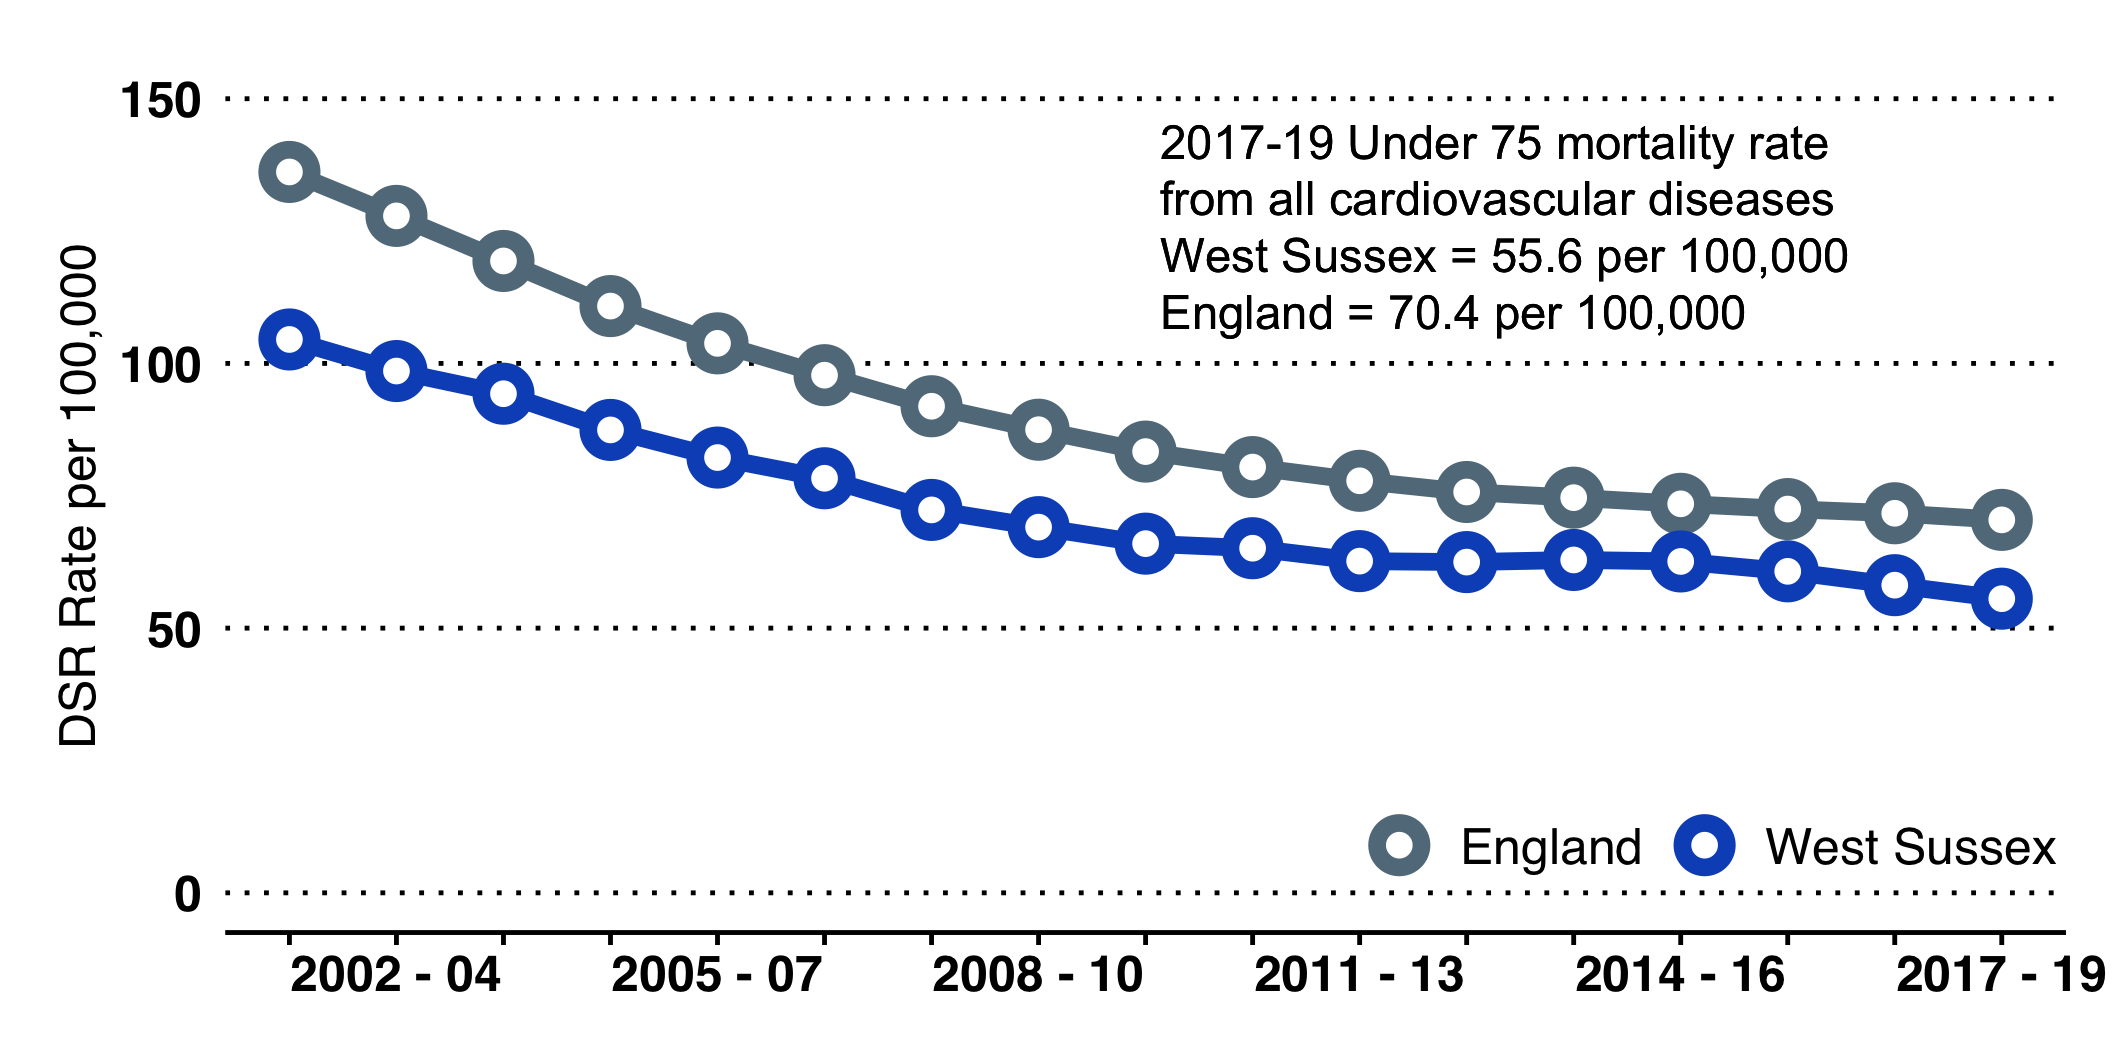
\includegraphics[width=.95\linewidth]{images/u75_cvd_line_3y.png}
    \label{fig:u75_cvd}
\end{figure}

Cardiovascular disease (CVD) remains a major cause of premature mortality. The rate has reduced greatly over the last 20 years, due to lifestyle improvement and treatment. The mortality rate in West Sussex is significantly better than the England rate\footnote{PHOF reference E04a}. 

\begin{figure}[htp]
    \caption[Age-standardised mortality rate (under 75 years) - Cancer]{Age-standardised mortality rate (under 75 years) - Cancer}
    \centering
    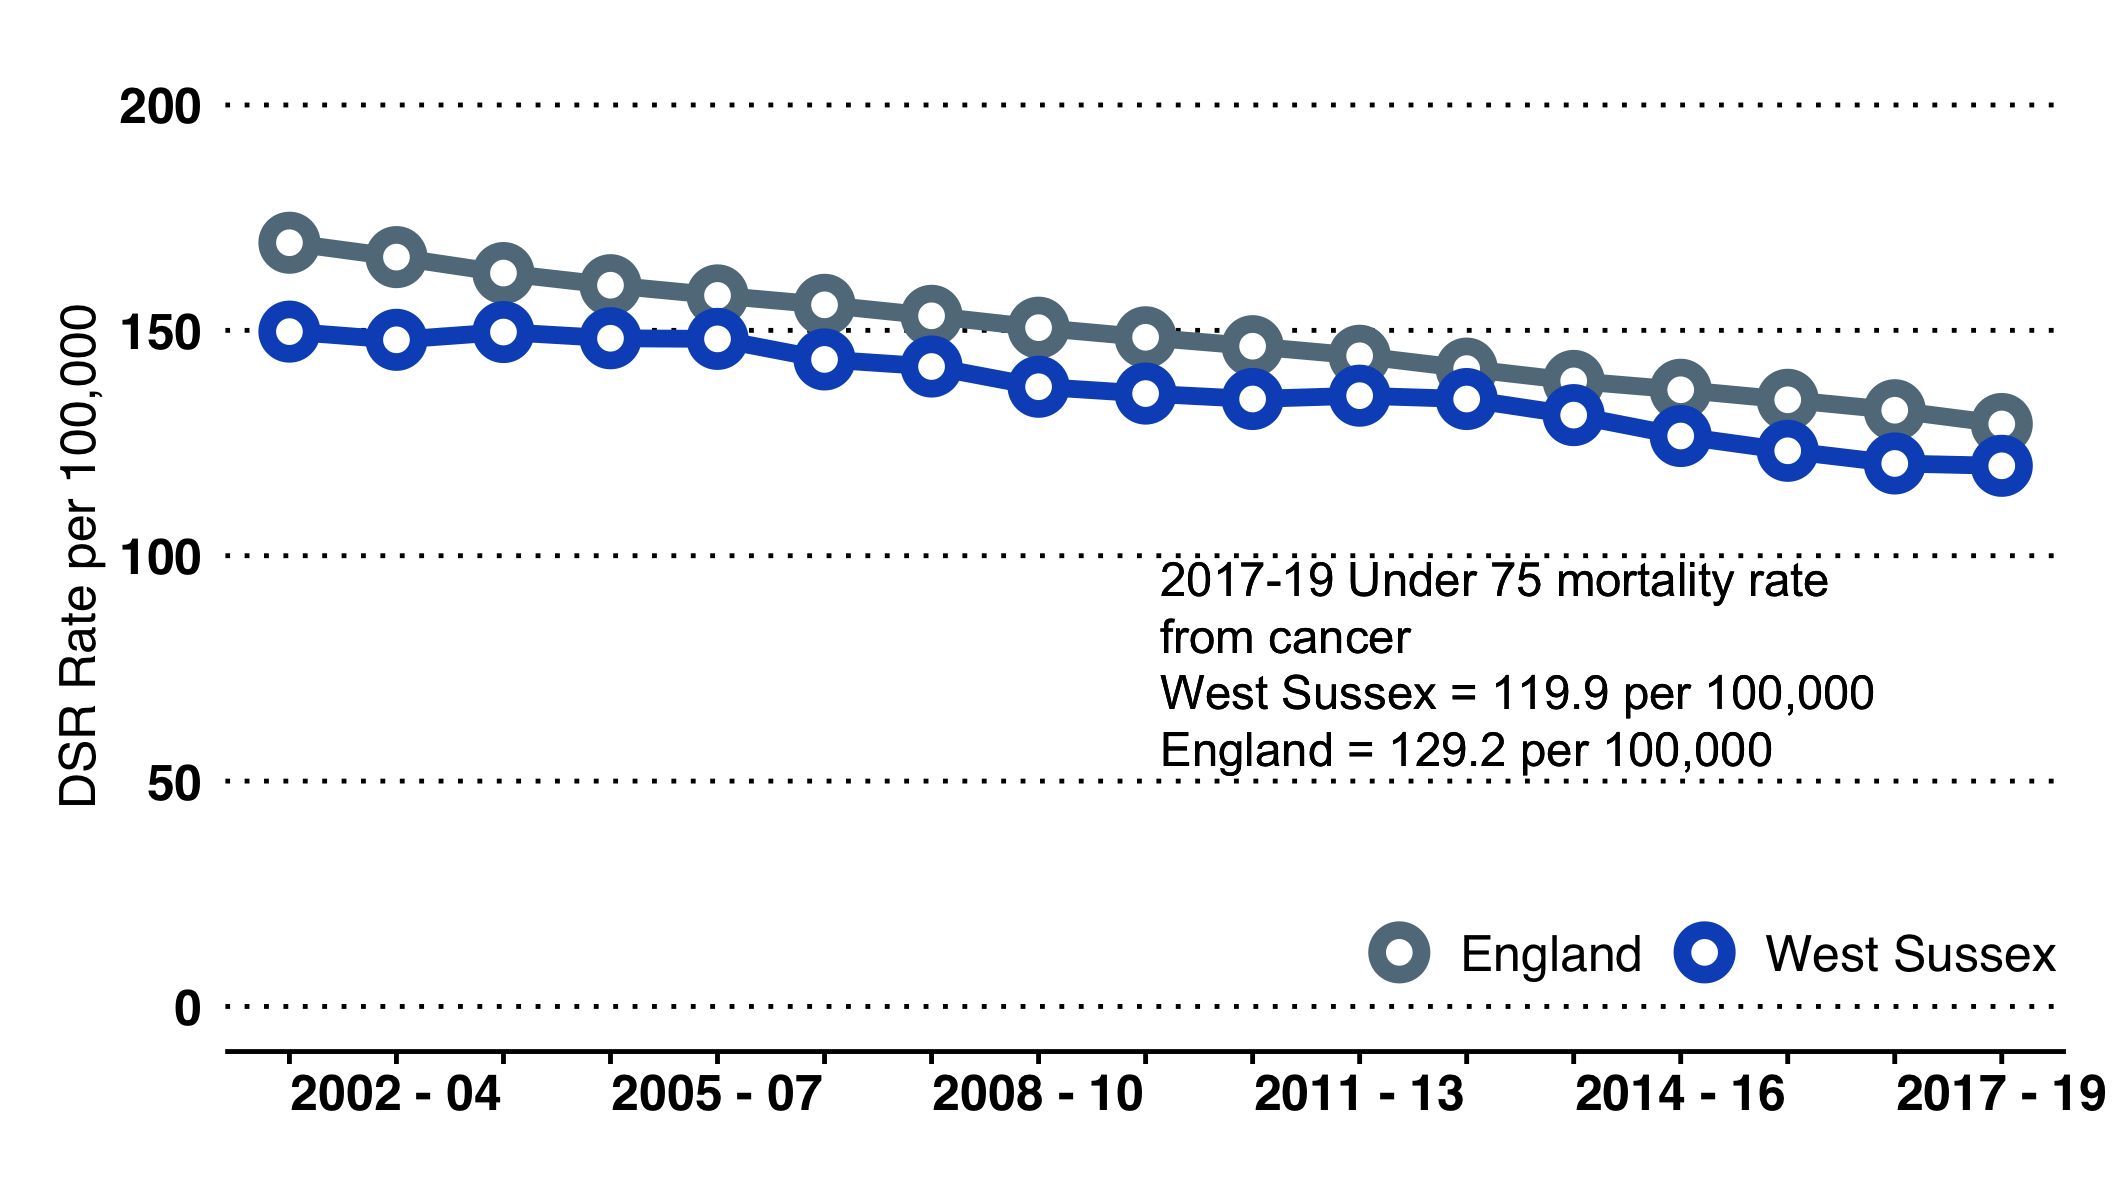
\includegraphics[width=.95\linewidth]{images/u75_cancer_line_3y.png}
    \label{fig:u75_cancer}
\end{figure}

Cancer remains the biggest cause of death for people under 75. A continued reduction will require sustained effort on prevention, early diagnosis and treatment. The rate in West Sussex is significantly better than the England rate\footnote{PHOF reference E05a}.

\begin{figure}[htp]
    \caption[Age-standardised mortality rate (under 75 years) - Liver Disease]{Age-standardised mortality rate (under 75 years) - Liver Disease}
    \centering
    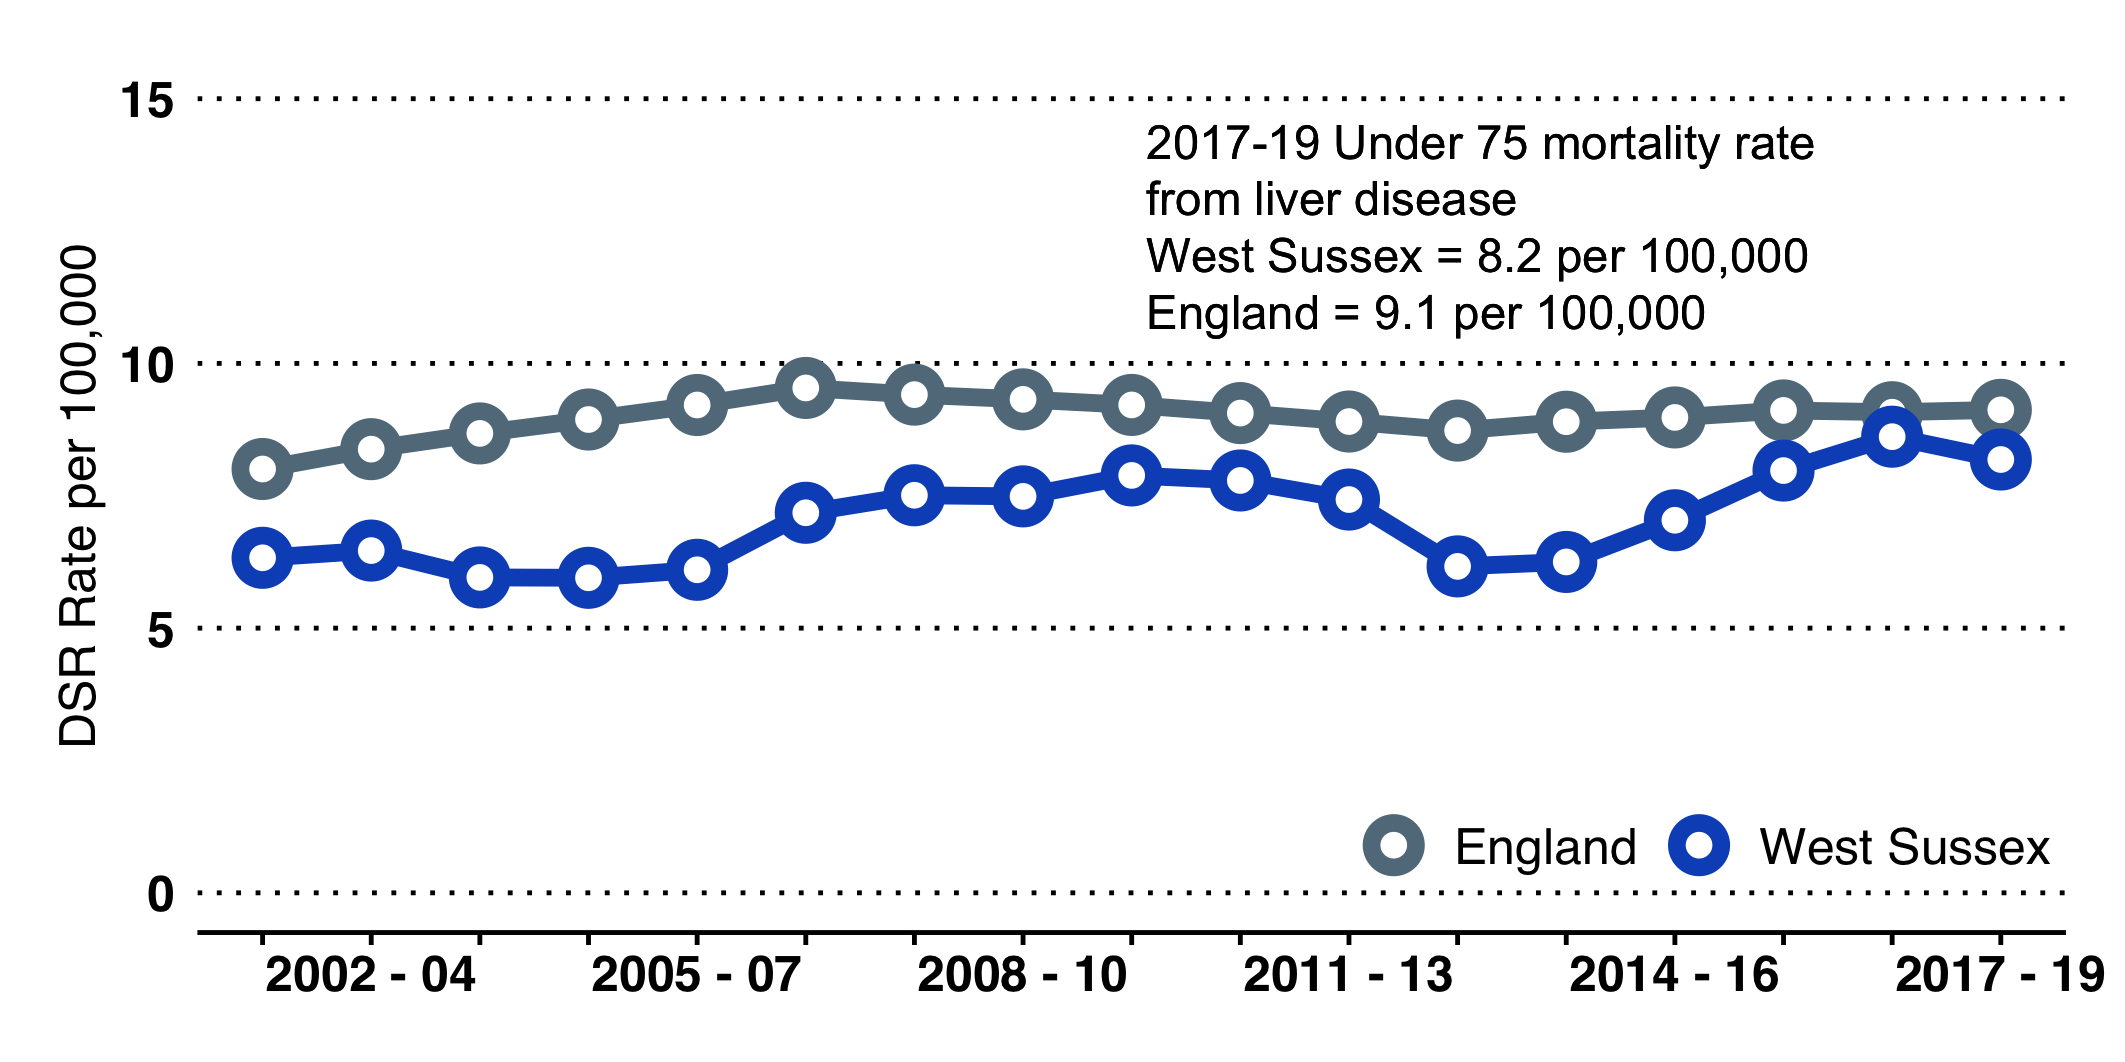
\includegraphics[width=.95\linewidth]{images/u75_liver_line_3y.png}
    \label{fig:u75_liver_b}
\end{figure}

Liver disease is a major cause of premature death. Most liver disease is preventable; both alcohol consumption and obesity are underlying factors, amenable to public health interventions. Of the major causes, the rate of mortality is not reducing. Locally the rate is below England\footnote{PHOF reference E06a}. 

\begin{figure}[htp]
    \caption[Age-standardised mortality rate (under 75 years) - Respiratory Disease]{Age-standardised mortality rate (under 75 years) - Respiratory Disease}
    \centering
    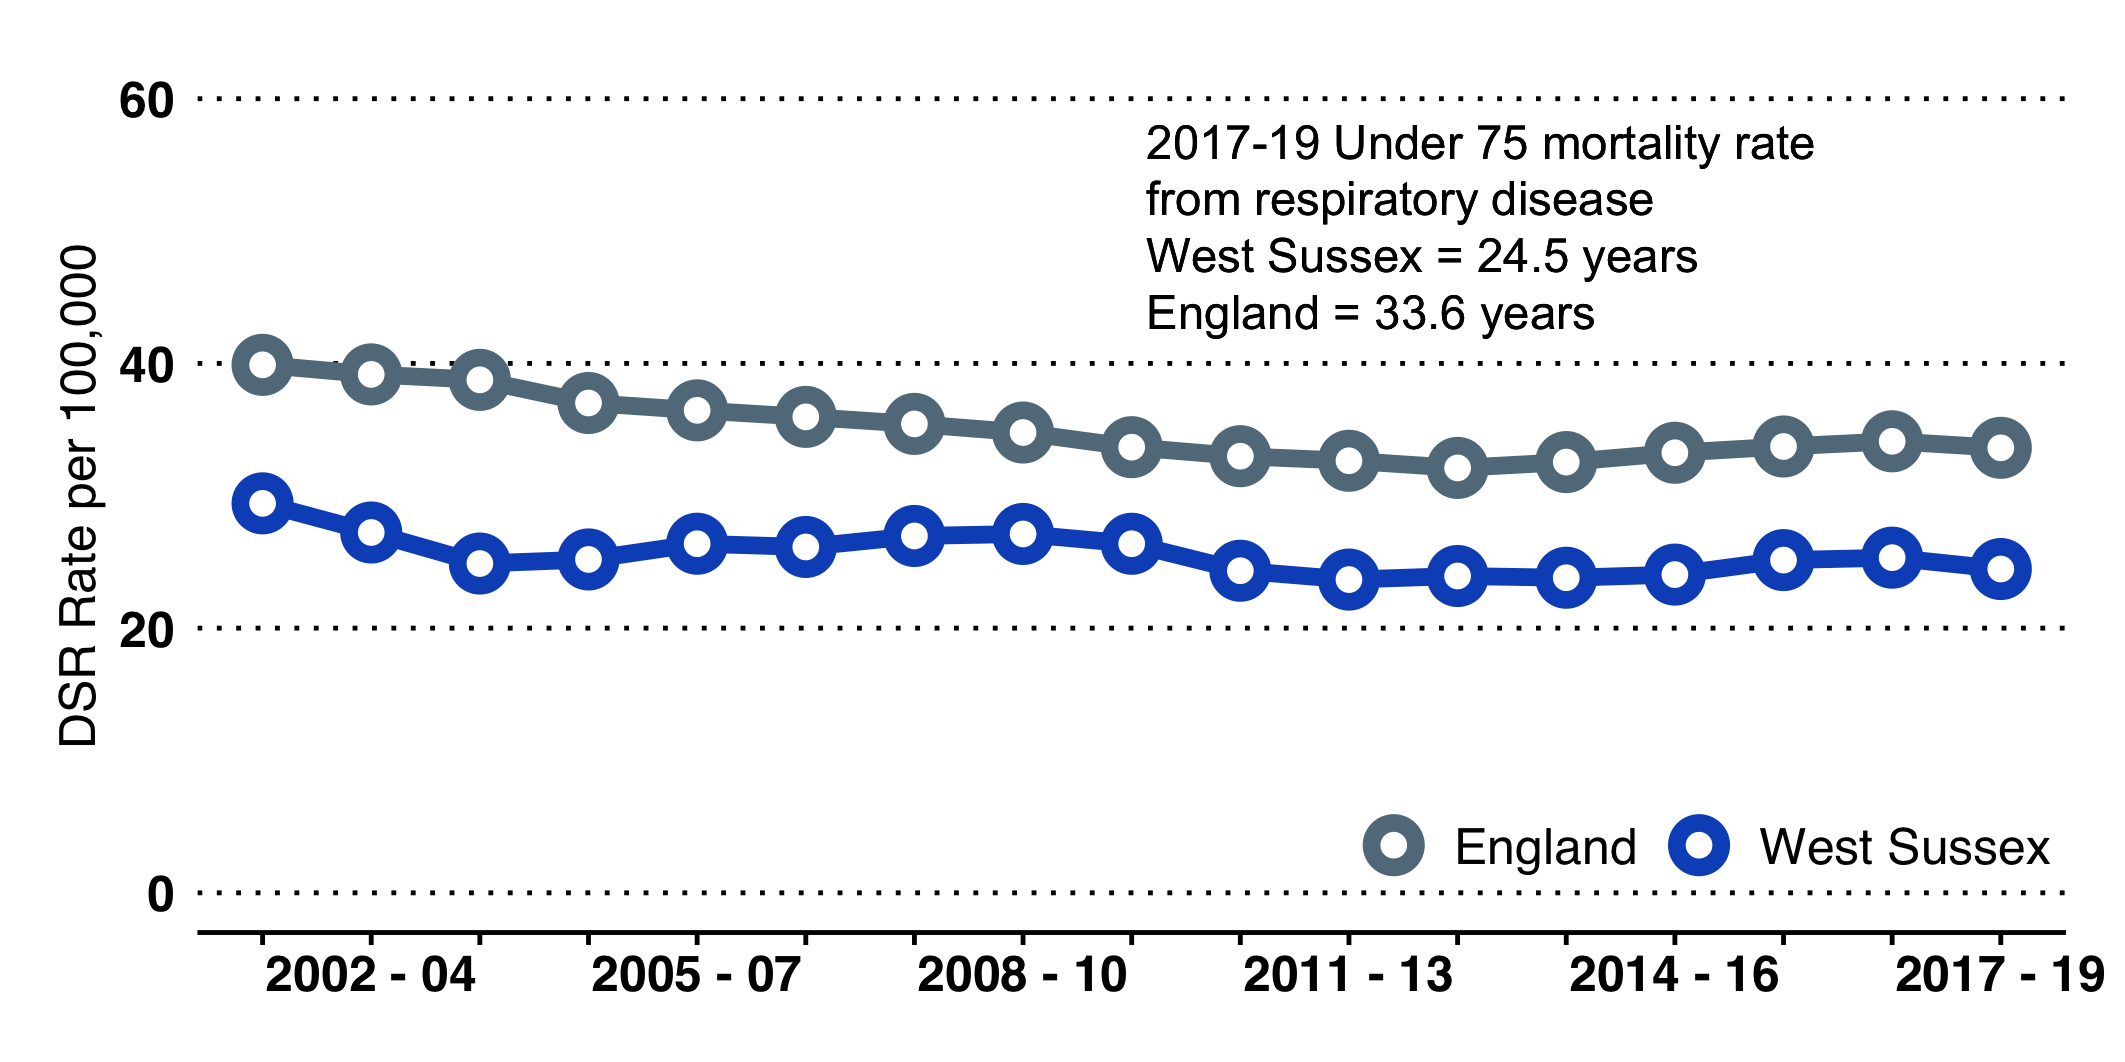
\includegraphics[width=.95\linewidth]{images/u75_respiratory_line_3y.png}
    \label{fig:u75_resp}
\end{figure}

Respiratory disease is a major cause of premature mortality. For chronic obstructive pulmonary disease (COPD), one of the main respiratory diseases, smoking is a major cause. The West Sussex rate is below that of England\footnote{PHOF reference E07a}. 

\clearpage

\subsection{Suicide}
The West Sussex Public Health and Social Research Unit carried out a Suicide Audit in 2017, covering suicides in the years 2013 to 2015. The audit provided detailed background context and circumstances and was undertaken to inform the local Suicide Prevention Strategy. The panel opposite details some of the background observations; for more detailed analysis please refer to the report or contact: Robert Whitehead (\url{robert.whitehead@westsussex.gov.uk}).

\begin{figure}[htp]
    \caption[Age-standardised mortality rate from suicide and injury of undetermined intent per 100,000 population (all ages) over time]{Age-standardised mortality rate from suicide and injury of undetermined intent per 100,000 population (all ages) over time\footnote{PHOF reference E10}.}
    \centering
    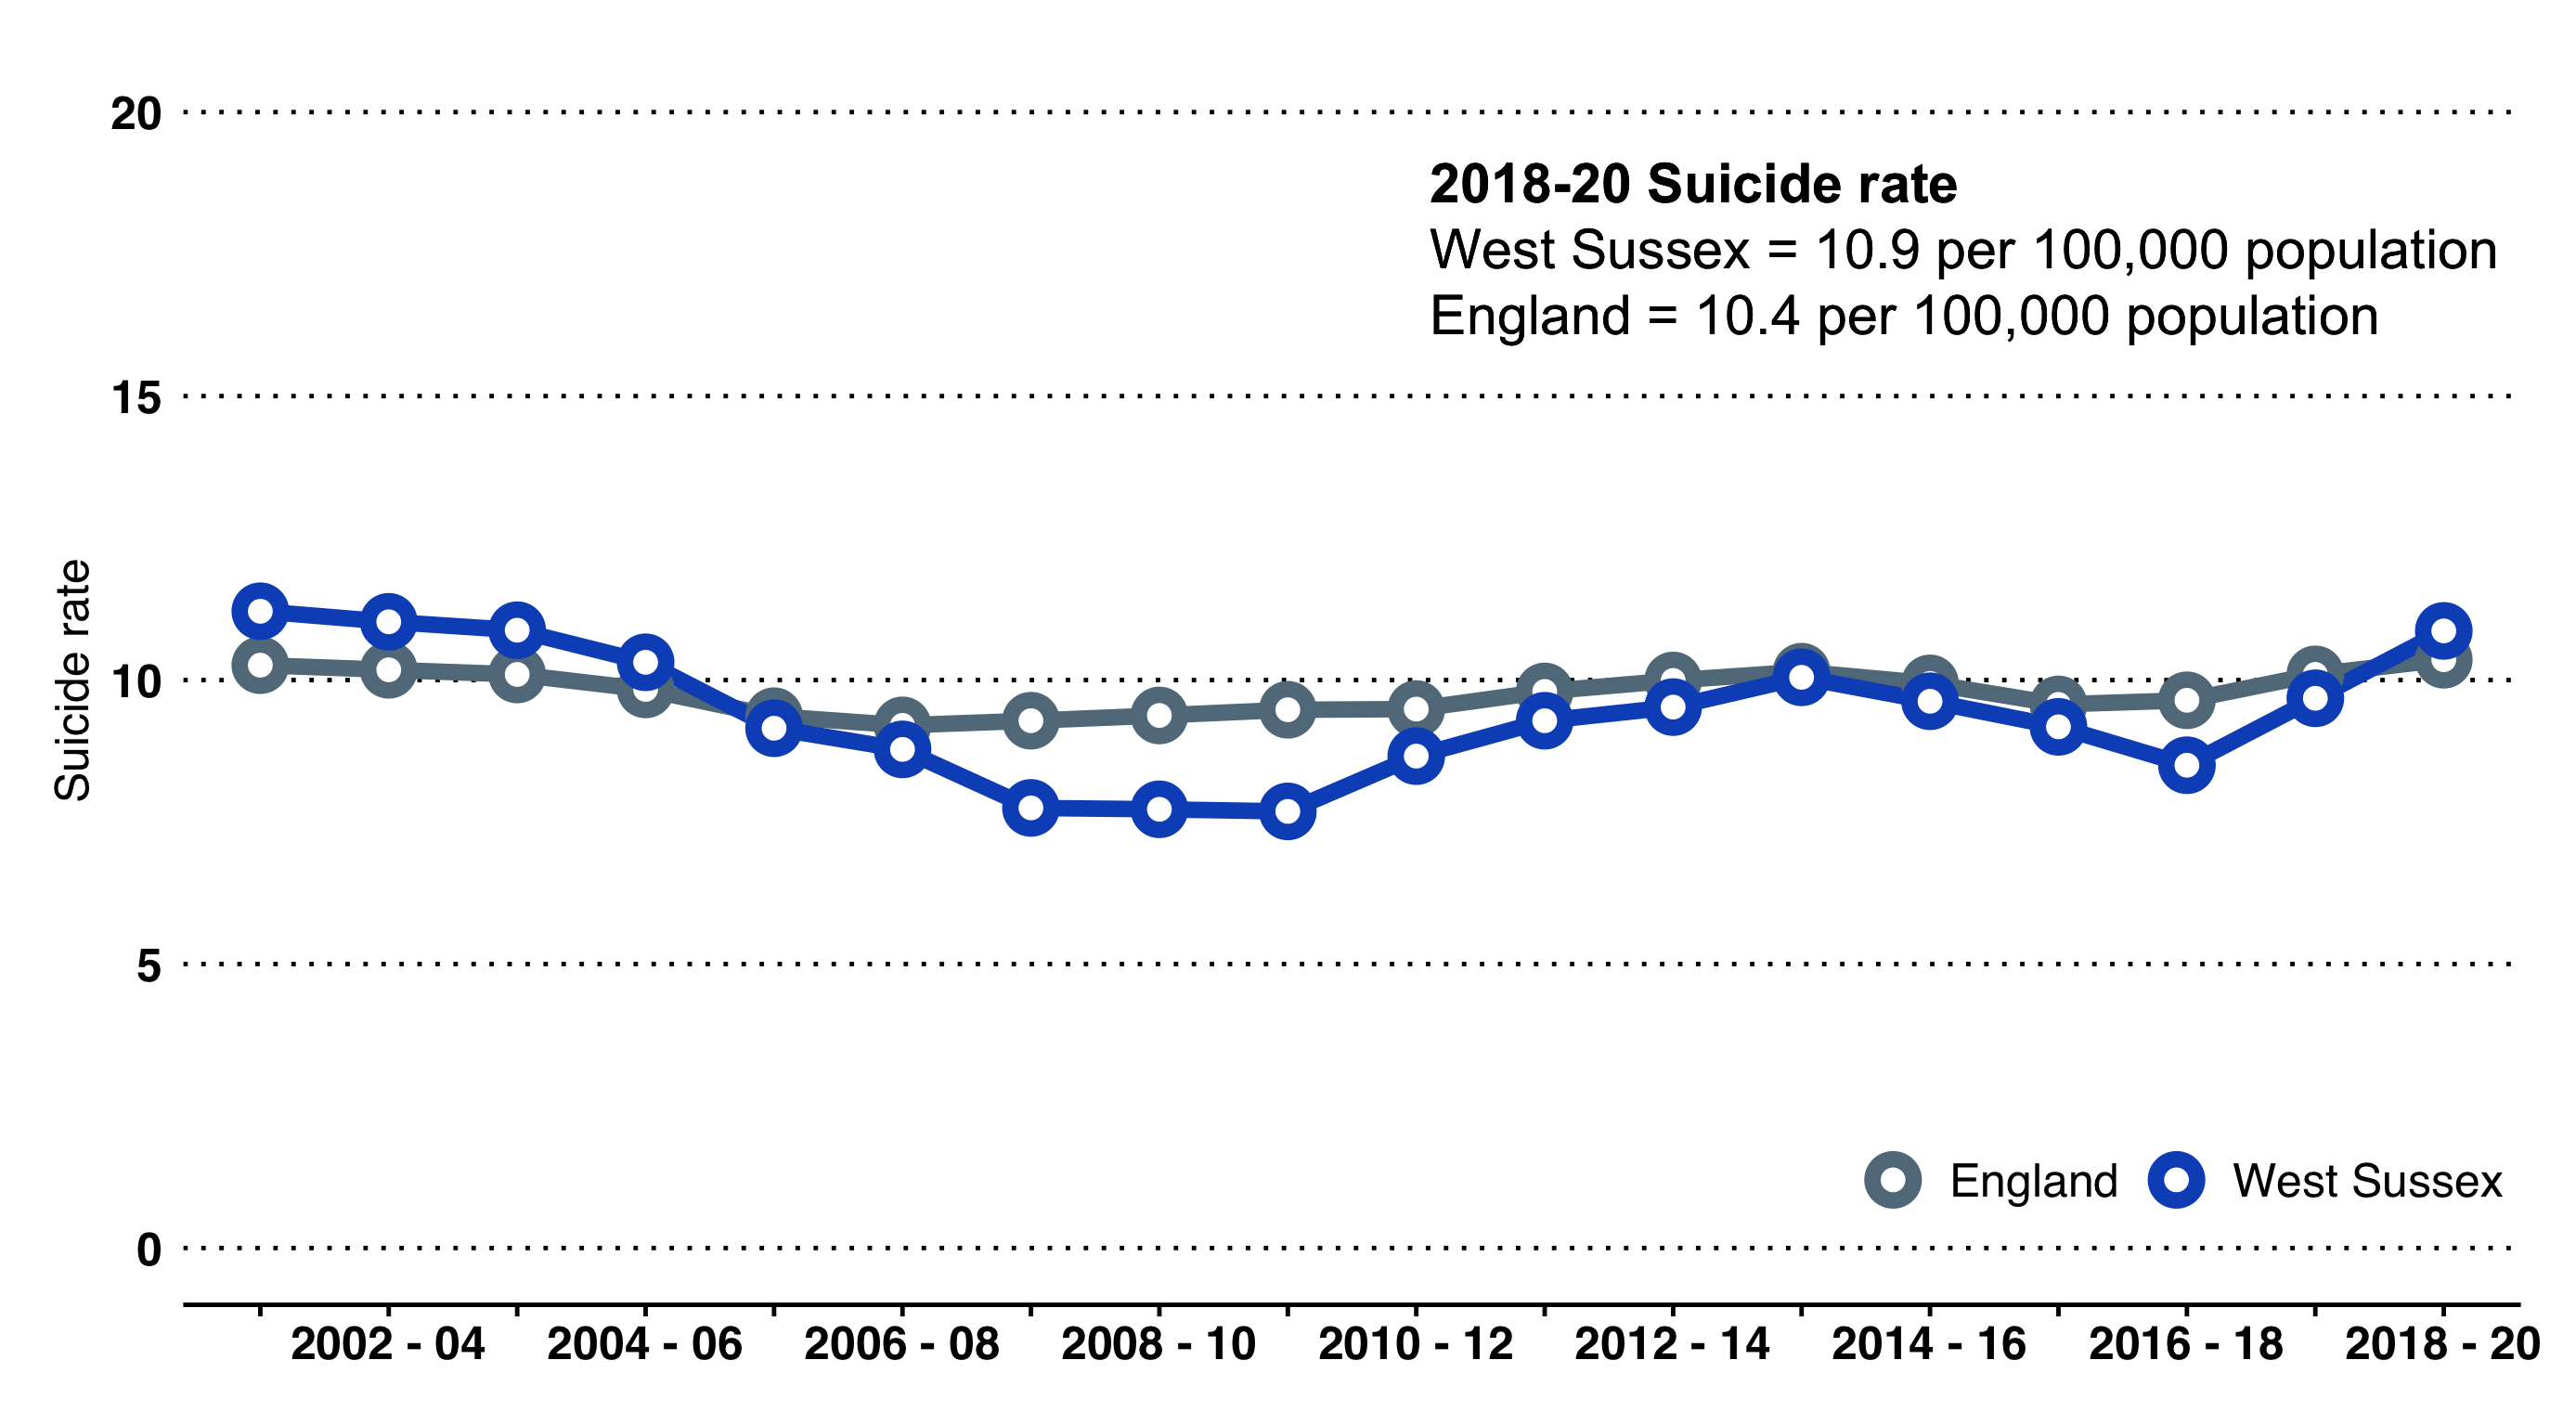
\includegraphics[width=\linewidth]{images/suicide_line.png}
    \label{fig:suicide}
\end{figure}

\subsubsection{Demographic Information from the West Sussex Suicide Audit 2013-15} For the years 2013-15 inclusive, there were 190 confirmed suicides and 23 open verdicts likely to be suicides.
\begin{itemize}[noitemsep]
    \item Combined, there were 52 females and 161 males included in the audit.
    \item Seasonal variations show a higher prevalence in summer months, though it is possible that this is random error found in low sample numbers.
    \item Nearly a third of male deaths and female deaths occurred between the ages of 45 and 54. Roughly half of female deaths and a fifth of male deaths occurred in those aged 65 and over.
    \item One in three individuals lived alone at the time of death and one in four lived with their spouse or partner.
    \item The most common means of suicide was by hanging or strangulation (43\%). Following this was self-poisoning (20\%), more frequent in older females, then impacts with a train (10\%), more frequent with younger males.
    \item Rail crossings are as common for suicide as rail stations (together accounting for 10\% of deaths).
    \item Over half of suicides occur in the home or elsewhere on the premises.
    \item Nearly one in three deaths occurred after consuming some level of alcohol. One in seven had taken illicit or non-prescribed drugs.
\end{itemize}

\subsection{Community Safety}
\subsubsection{Violent offences} Violent offences (measured per 1,000 population)\footnote{PHOF reference B12b}  more than doubled in West Sussex the last six years to 2018/19, in line with national rises. While no longer increasing as quickly, numbers and rates of violent offences in West Sussex remain high. In 2020/21, there were 18,454 recorded offences, compared with 7,448 in 2013/14.

The rate in West Sussex (21.8 per 1,000 population) remains lower than England (29.5 per 1,000) and most comparable authorities. However, the Crawley rate (35.1 per 1,000) exceeds both West Sussex and England, though this has fallen since 2019/20.

% \begin{figure}[htp]
%     \caption[Violent offences per 1,000 population (all ages) in West Sussex districts and boroughs.]{Violent offences per 1,000 population (all ages) in West Sussex districts and boroughs.\footnote{PHOF reference B12b}.}
%     \centering
%     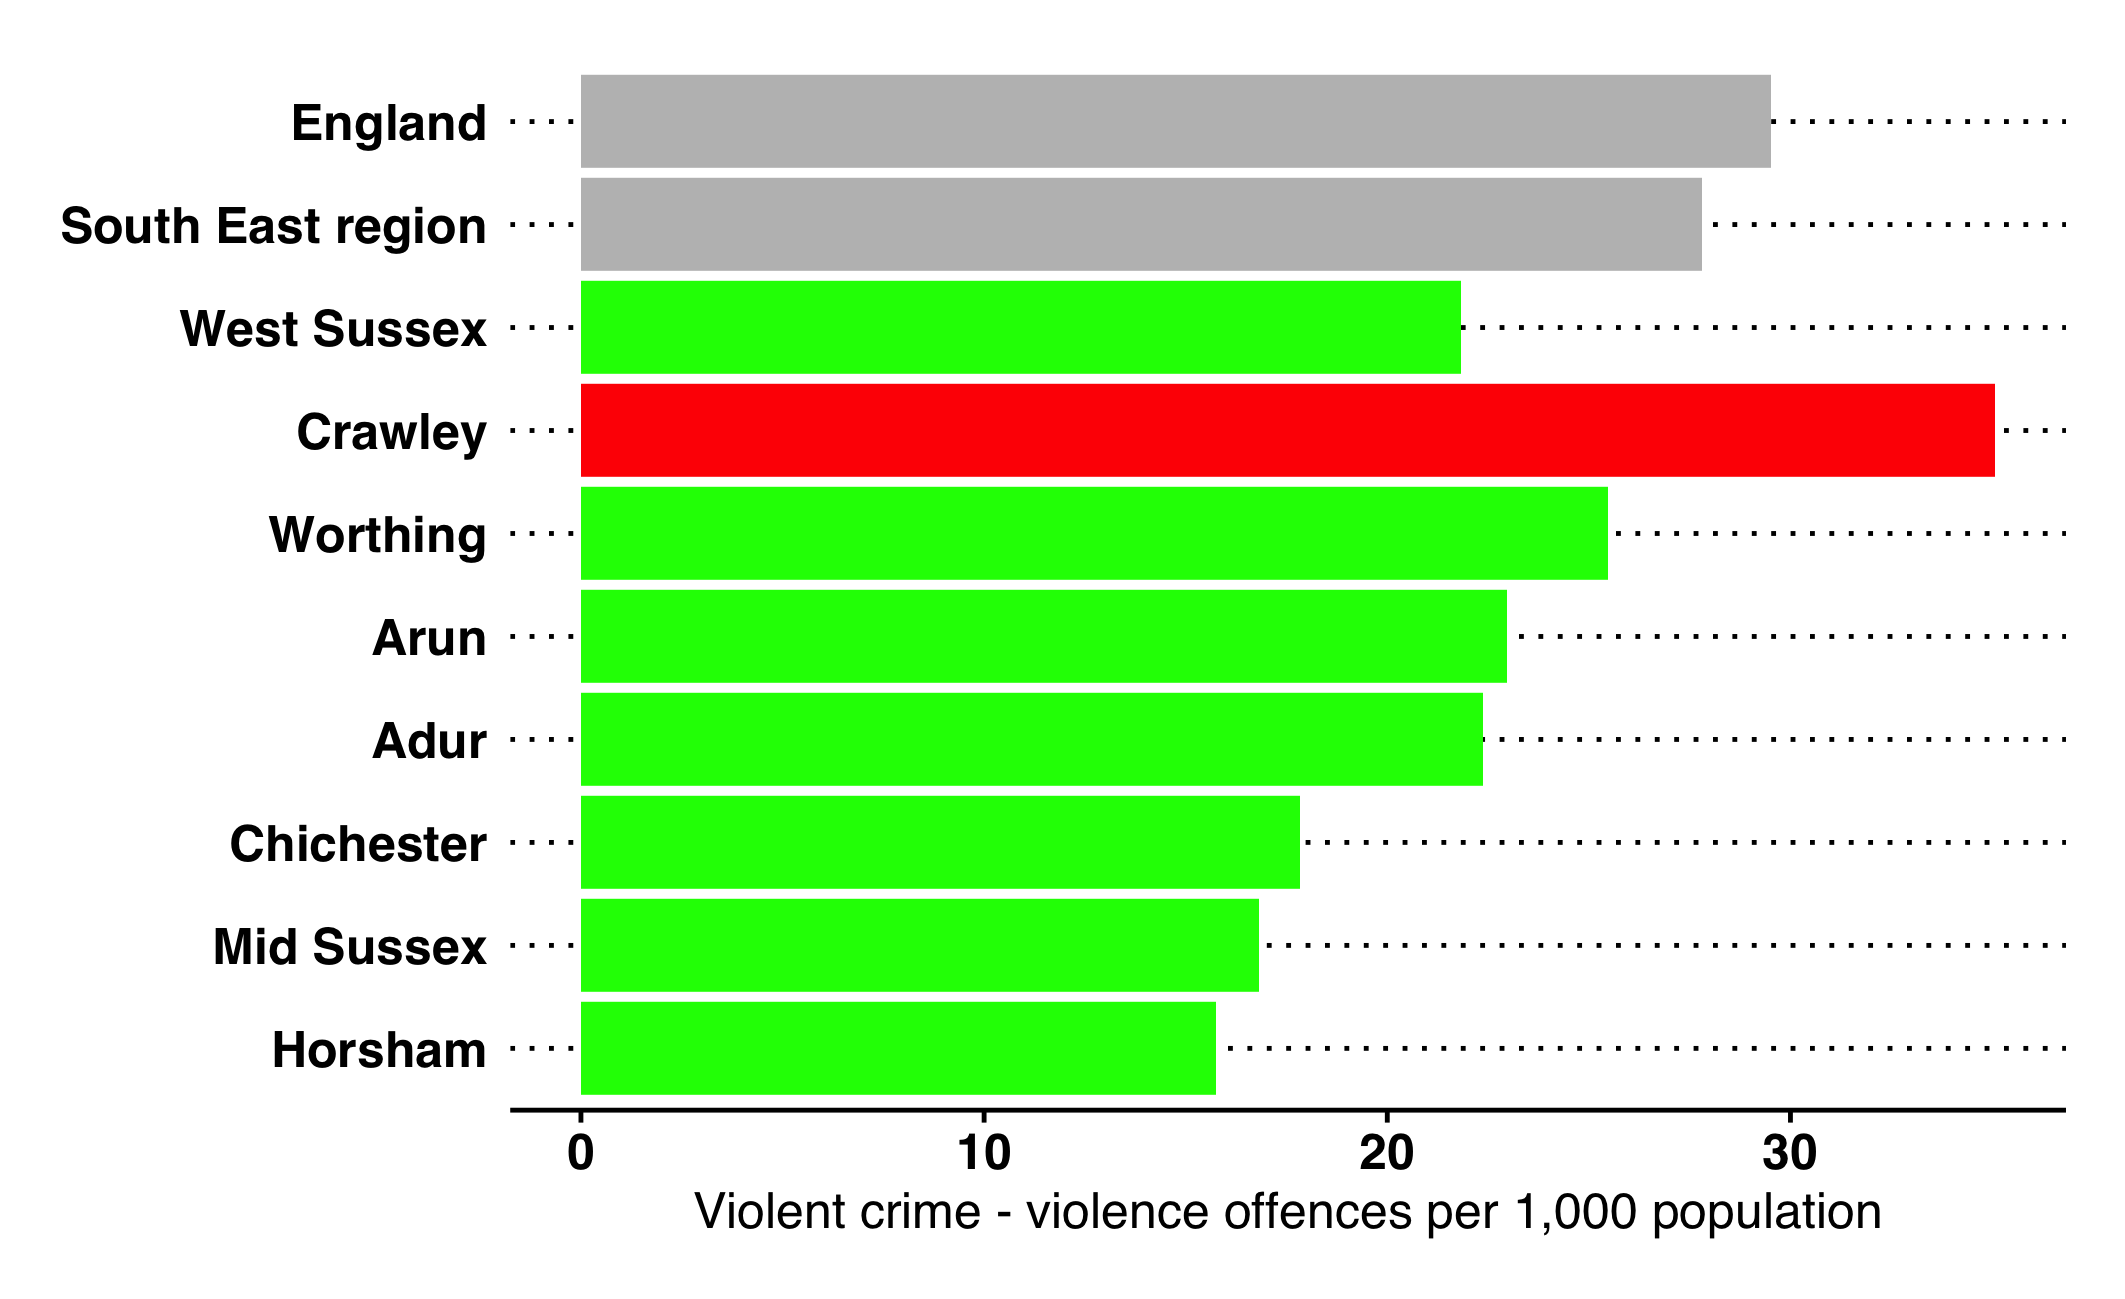
\includegraphics[width=\linewidth]{images/violent_offences_bar.png}
%     \label{fig:suicidviolence:ltla}
% \end{figure}

% FIGURE - LTLA Rate per 1,000 population

% \begin{figure}[htp]
%     \caption[Violent offences per 1,000 population (all ages) over time]{Violent offences per 1,000 population (all ages) over time compared to England.\footnote{PHOF reference B12b}.}
%     \centering
%     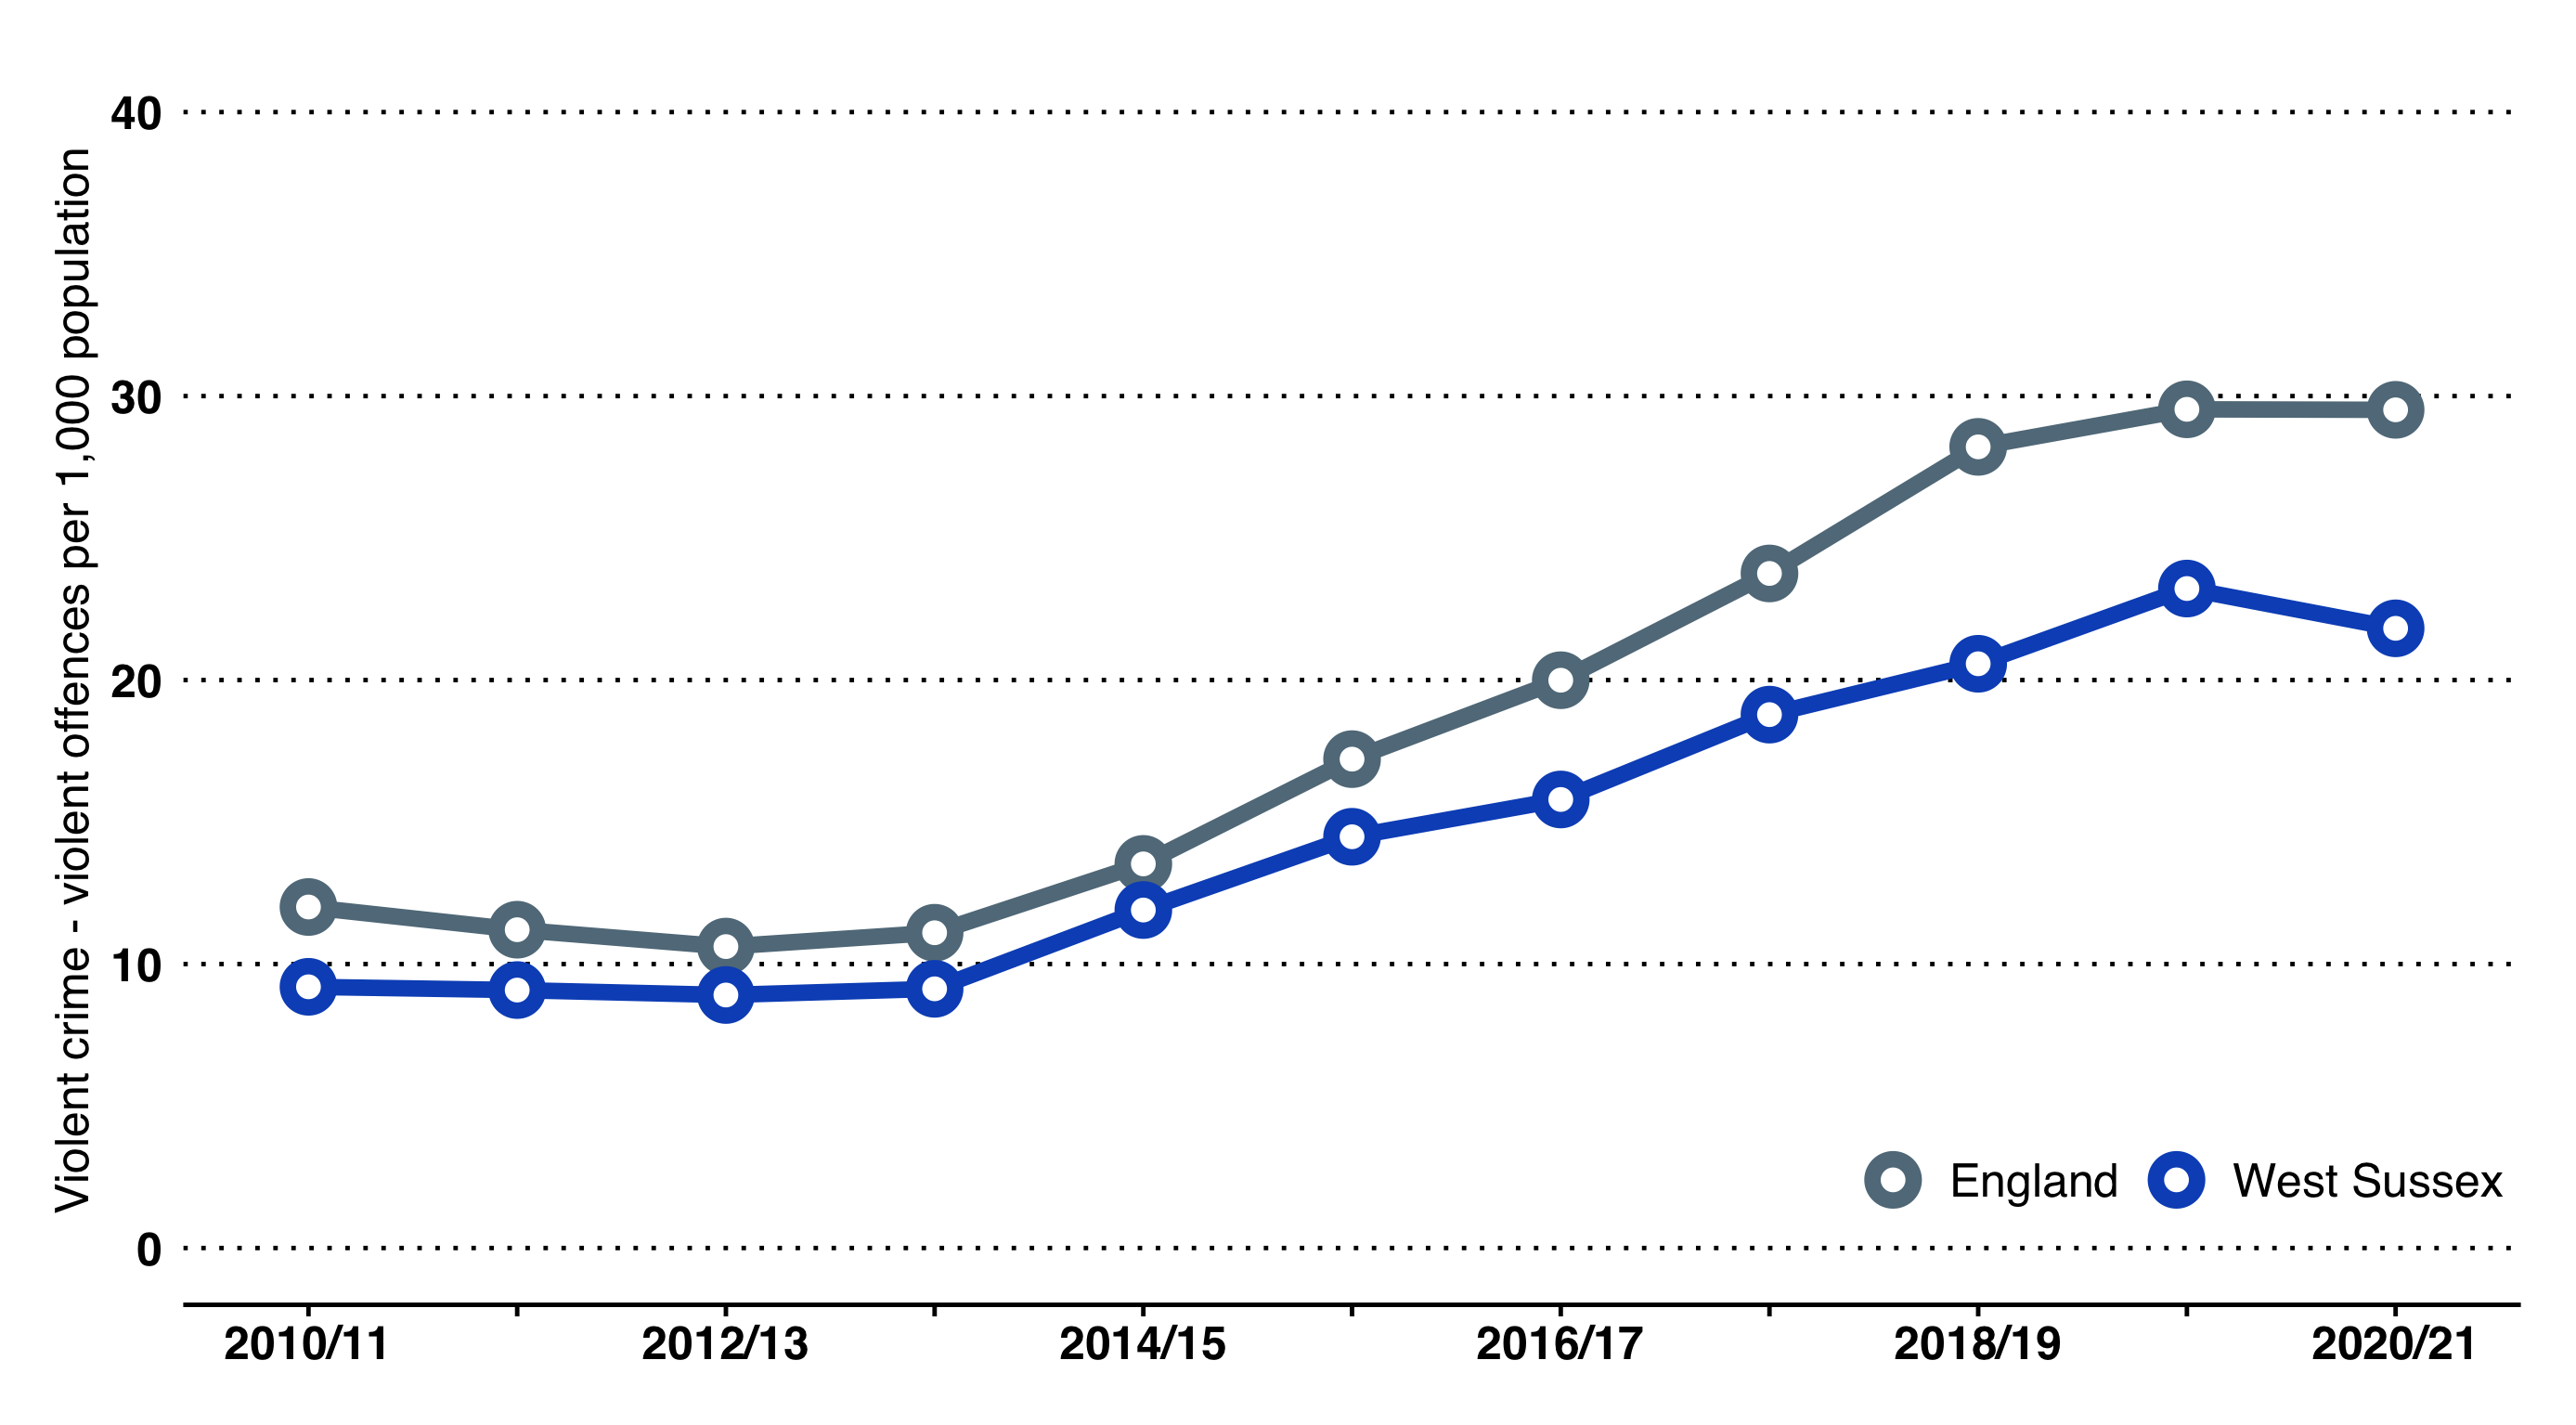
\includegraphics[width=\linewidth]{images/violent_offenses_line.png}
%     \label{fig:violence:time}
% \end{figure}

\subsubsection{Sexual offences} Sexual offences (measured per 1,000 population)\footnote{PHOF reference B12c} have also more than doubled in West Sussex over the last eight years, in line with national rises. In 2020/21, there were 1,602 recorded sexual offences, compared with 697 in 2013/14 (though a decrease on 2019/20).

The rate in West Sussex (1.9 per 1,000 population) remains lower than England (2.3 per 1,000) and is the seventh lowest amongst CIPFA neighbours. Crawley exceeds the national and West Sussex rates, at 2.8 per 1,000.

% FIGURE - Rate per 1,000 population over time (West Sussex vs South East vs England)

% \begin{figure}[htp]
%     \caption[Sexual offences per 1,000 population (all ages) over time]{Sexual offences per 1,000 population (all ages) over time compared to England.\footnote{PHOF reference B12c}.}
%     \centering
%     \includegraphics[width=\linewidth]{images/sexual_offences_line.png}
%     \label{fig:sexual_off:time}
% \end{figure}

\subsubsection{Domestic abuse} In 2020/21, the rate of domestic abuse-related incidents and crime\footnote{PHOF reference B11. Note that local authorities are allocated the rate of the police force within which they sit.} was 22.1 per 1,000 in West Sussex, significantly below the national rate of 30.3 per 1,000 and one of the lowest amongst CIPFA neighbours.

\subsubsection{Road accidents} Whilst the national number of people killed or seriously injured (KSI) on roads\footnote{PHOF reference B10.} has remained stable in recent years, there has been an upward trend in West Sussex. At 131.0 per billion vehice miles (equal to 576 people in 2019 and 505 people in 2020), West Sussex has one of the highest KSI rates in the country (England 86.1 per billion vehicle miles). Note that Figure~\ref{fig:ksi:dabs} refers to historic data, as no information are available for districts and boroughs post-2020.

% \begin{figure}[htp]
%     \caption[number of people killed or seriously injured (KSI) on roads per 1,000 population (all ages) over time]{Number of people killed or seriously injured (KSI) on roads per 1,000 population (all ages) in West Sussex districts and boroughs, compared to England.\footnote{PHOF reference B10}.}
%     \centering
%     \includegraphics[width=\linewidth]{images/road_accidents_rag.png}
%     \label{fig:ksi:rag}
% \end{figure}

\begin{figure*}
    \caption[Community safety indicators in West Sussex.]{Community safety indicators in West Sussex.}\label{fig:com-safety-inds}
    \vspace*{3mm}
    \centering
    \begin{subfigure}[t]{0.45\textwidth}
        \caption{Number of people killed or seriously injured (KSI) on roads in West Sussex districts and boroughs, compared to England (PHOF reference B10).}\label{fig:ksi:dabs}
        \centering
        \includegraphics[width=.7\textwidth]{images/road_accidents_rag.png}
    \end{subfigure}
    \begin{subfigure}[t]{0.45\textwidth}
        \caption[Violent offences per 1,000 population (all ages) in West Sussex districts and boroughs.]{Violent offences per 1,000 population (all ages) in West Sussex districts and boroughs (PHOF reference B12b).}\label{fig:violence:ltla}
        \centering
        \includegraphics[width=.7\textwidth]{images/violent_offences_bar.png}
    \end{subfigure}
    \begin{subfigure}[t]{0.45\textwidth}
        \caption[Violent offences per 1,000 population (all ages) over time]{Violent offences per 1,000 population (all ages) over time compared to England (PHOF reference B12b).}\label{fig:violence:time}
        \centering
        \includegraphics[width=\textwidth]{images/violent_offenses_line.png}
    \end{subfigure}
    \begin{subfigure}[t]{0.45\textwidth}
        \caption[Sexual offences per 1,000 population (all ages) over time]{Sexual offences per 1,000 population (all ages) over time compared to England (PHOF reference B12c).}\label{fig:sexual_off:time}
        \centering
        \includegraphics[width=\textwidth]{images/sexual_offences_line.png}
    \end{subfigure}
\end{figure*}

\clearpage

% FIGURE - LTLA Rate per 100,000 population


% \subsection{Further information}

% This is a summary document; more detailed local analyses (alongside a whole host of national profiles!) are available, including the needs assessment and briefings highlighted below. If you have specific information requests please contact the team.

% In addition to the contacts shown in the summary, overall for overall queries for Living Well in the West Sussex Public Health and Social Research Team contact Jacqueline Clay - (\url{jacqueline.clay@westsussex.gov.uk}) % Living well
\newpage
\section{Ageing Well}
\subsection{Summary}

West Sussex is home to [192,900] people aged 65 years or over. Overall, older people in the county are relatively healthy and the county is a good place to live. More people are continuing in paid employment well past the "traditional" retirement age, and older people provide considerable caring support to their families and friends, and the wider community.

The number of older people is projected to increase and to do so at a greater rate than the overall population increase. It will be increasingly important that services, communities and families work together to support older people and their families to remain healthy, happy and at home in the community. To have a healthy older population it is important that the wider determinants of health (housing, planning, income, education etc) are conducive to better ageing, and that organisations and communities work together to promote good health in mid-life, prevent the onset of long- term conditions, and support self-care of health and self-management of conditions.

Overall, health and wellbeing outcomes are good for all life stages in West Sussex, including later life. However, as with the earlier lifestages, the average hides the considerable inequalities in the county.

Life expectancy overall has continued to increase but with healthy life expectancy stalling, this means that more of life is being spent in poor health or with a disability. Male life expectancy still lags behind female life expectancy (80.8 years compared with 84.2 years) and is far lower amongst people from the most deprived and disadvantaged groups, including older people living in poverty and people with a learning disability and/or mental health condition.

The importance of the quality of life lived, not just the length of life, is central to the priorities identified in the West Sussex Health and Wellbeing Strategy 2019-24. Loneliness and social isolation in later life have been identified, through national and local surveys, as impacting the quality of life and are linked to physical health outcomes. Although it should be stressed that the impact of loneliness is not restricted to this age group, it is a life stage when mobility and the opportunity for social contact can decline.

Locally, outcomes relating to falls have fluctuated and often have been poorer compared with comparable authorities; in 2018/19 there were over 5,000 emergency hospital admissions due to falls. At 2,416 per 100,000, this rate is significantly higher than England and the second highest amongst comparable authorities. Of specific concern were the 840 hip fractures in residents aged 80+ years, as, for many older people, such an injury may result in moving into residential care.

Most care is self-care. To self-care and self-manage long-term conditions, people of all ages need access to good advice and may need additional support. Data from the GP Patient Survey found that, across West Sussex, [85\% of people said that they were 'fairly' or 'very' confident in managing their conditions] but there is variation across the county and confidence tends to decline with age. In terms of support from local organisations and services, compared to working age adults with a health condition, older people were more likely to say they had enough support.

Just as the quality of birth is valued at the start of life, support for the end of life was identified as a priority by the West Sussex Health and Wellbeing Board. There is again considerable variation across the county; notably, the percentage of people dying at home remains low in Crawley, when compared with the rest of the county and England overall.

\subsection{Over 65 Population Background}
\paragraph{Population aged 65 years or over} In 2018, there were an estimated 195,500 people aged 65 years or over in West Sussex, compared with 159,200 in 2008. In 2028, ONS project that there will be 241,300 people in this age group in West Sussex, with the average year-on-year change increasing from 3,600 in the last 10 years to over 4,700 in the next 10 years.

FIGURE Year-on-year change in the number of 65+ year-olds in West Sussex (graph)

\begin{itemize}[noitemsep]
    \item Over 30\% of people aged 65 years or over live alone, representing over 52,000 people and 15\ of all households in West Sussex.
    \item Over 7,700 people aged 65 years or over live in residential or nursing care.
    \item Over 27,500 people aged 65 years or over are providing unpaid care for a family member, friend and/or neighbour, with over 9,000 providing unpaid care for 50+ hours a week (and of these, 1,300 are estimated to be aged 85 years or over).
    \item West Sussex has a high rate of home ownership, with over 80\% of older people being home owners.
    \item It is estimated that over 38,000 older people (~20\%) in the county have mobility problems (such as going out of doors and walking down the road; getting up and down stairs; getting around the house on the level; getting to the toilet; getting in and out of bed).
\end{itemize}

\begin{tcolorbox}[title={Loneliness - identifying risks at a neighbourhood level}, colback={boxcolour}]
{\bf Loneliness} is the subjective feeling of a gap between someone's desired and actual social contact. Linked to quality of contacts. Loneliness is not desired by the person experiencing it.

{\bf Social isolation} is an objective measure of contact with others, usually measured in quantitative terms. Some people may choose to have few contacts.

Age UK have produced maps of areas where people may be at greater risk of loneliness. The maps reflect four underlying indicators taken from the 2011 Census: 

\begin{itemize}[noitemsep]
    \item marital status
    \item self-reported health status
    \item age
    \item household size
\end{itemize}

Age UK state that the four factors predicted around 20\% of the loneliness observed amongst people aged 65+. This was established by work undertaken as part of the English Longitudinal Study of Ageing (ELSA). Age UK state that their map should be used alongside local knowledge and understanding of the local population.\footnote{\url{https://www.ageuk.org.uk/our-impact/policy-research/loneliness-research-and-resources/loneliness-maps/}}
\end{tcolorbox}

FIGURE - screenshot of the maps in action

\subsection{Long Term Health Conditions}
\paragraph{Older people with long term conditions} Estimates of the number of older people living with a long term condition are based on prevalence assumptions from national research\footnote{The POPPI website from IPC has been used for the estimates.}. Note: these are broad rounded estimates

\begin{itemize}[noitemsep]
    \item People aged 65+ predicted to have diabetes - 24,000
    \item People aged 65+ estimated to have dementia - 14,300\footnote{The estimated dementia diagnosis rate in over-65s is a PHOF indicator (E15)}
    \item People aged 65+ predicted to have depression - 16,650
    \item People aged 65+ predicted to have severe depression - 5,300
    \item People aged 65+ predicted to have a longstanding health condition caused by bronchitis and emphysema - 3,200
    \item People aged 65+ predicted to have a longstanding health condition caused by a stroke - 4,500
    \item People aged 65+ predicted to have a bladder problem at least once a week - 31,900
    \item People aged 65+ predicted to have a fall - 52,200
    \item People aged 65+ predicted to be admitted to hospital as a result of a fall - 4,100
    \item People aged 65+ predicted to have severe hearing loss - 15,600
    \item People aged 75+ predicted to have registrable eye conditions 6,200
\end{itemize}

In relation to recorded prevalence, approximately 9,148 people in West Sussex are on GP dementia registers, the majority (over 5,700) in the Coastal West Sussex CCG area.

\paragraph{Musculoskeletal problems (MSK)} In 2018/19, 16\% of people aged 18+ reported a long-term Musculoskeletal (MSK) problem\footnote{PHOF reference C27}, such as a long-term back pain or joint pain, representing over 110,000 people in West Sussex.

\paragraph{Sensory impairment} Independence in later life can be severely impacted by hearing and sight loss. Sensory impairment can act to increase loneliness and social isolation and hearing loss is a risk factor for dementia at older ages.

\begin{itemize}
    \item Around 18,000 people aged 65 years or over are estimated to have a moderate to severe visual impairment\footnote{Visual acuity (VA) of less than 6/18 (moderate or severe) is largely used as the point which approximates to the statutory threshold for qualifying as registered severely sight impaired (blind) or registered sight impaired (partially sighted).}. Of those over 75 years, approximately half are estimated to have "correctable sight loss", with conditions such as cataracts.
    \item 6,200 people aged 75 years or over are estimated to have a registrable eye condition.
    \item 17,000 people aged 65 years or over are estimated to have severe hearing loss\footnote{Hearing loss is measured by assessing the quietest sounds someone can hear using tones with different frequencies. In hearing tests, a person is asked to indicate when they can hear a tone; the level is then adjusted to find their threshold, when they can just hear it. Thresholds are measured in units called dBHL: dB stands for 'decibels' and HL stands for 'hearing level'. The greater the threshold level in dBHL, the worse the hearing loss. People with thresholds between 0 and 20 dBHL across all the frequencies are considered to have 'normal' hearing. The threshold of 25 dBHL indicates some hearing loss; the threshold of 65 dBHL indicates severe hearing loss. (adapted from POPPI Source: IPC)}.
    \item Sight loss due to age-related macular degeneration (AMD) in 65+ year-olds has increased in West Sussex in the last three years. In 2017/18, the rate in West Sussex was 131.7 per 100,000 and, having previously been lower than England, now exceeds the national rate and is the second highest amongst comparable local authorities. In 2017/18, there were 254 new Certifications of Visual Impairment (CVI), 70 more than 2016/17.
\end{itemize}

{\bf Preventable sight loss - age related macular degeneration (AMD)}
FIGURE Rate of new Certifications of Visual Impairment per 100,000 over-65s (graph)

\subsection{Multi-morbidity estimates}
\paragraph{Multi-morbidity Public Health Estimates} As we age we are likely to have or develop one or more long term health condition. This is called co-morbidity.

In 2018, Public Health England published estimates of the number of people with multi-morbidities in each lower tier authority in England. In doing this, PHE noted some challenges in how multi-morbidity is described, including how many and which conditions are included (physical and/or mental health conditions).

\begin{table*}
    \caption{Physical Conditions included in the PHE Estimates}
    \centering
    \begin{tabular}{ccc}
        \toprule
        Hypertension & Heart failure & Treated constipation\\
        Painful condition & Prostate disorders & Stroke \& transient Ischaemic attack\\
        Asthma (currently treated) & Glaucoma & Chronic kidney disease \\
        Coronary heart disease & Epilepsy (currently treated) & Diverticular disease of intestine \\
        Treated dyspepsia & Psoriasis or eczema & Viral Hepatitis \\
        Diabetes & Inflammatory bowel disease & Chronic liver disease \\
        Thyroid disorders & Migraine & Atrial fibrillation \\
        Rheumatoid athritis & Blindness \& low vision & Peripheral vascular disease \\ 
        Hearing loss & Chronic sinusitis & Parkinson's disease \\
        Chronic obstructive pulmonary disease & Irritable bowel syndrome & Multiple sclerosis \\
        Bronchiectasis & New diagnosis of cancer in last 5 years & \ \\
        \bottomrule
    \end{tabular}
    \label{tab:op:phys_conditions}
\end{table*}
\begin{table*}
    \caption{Mental Health Conditions included in the PHE Estimates}\
    \centering
    \begin{tabular}{ccc}
        \toprule
        Anorexia or bulimia & Anxiety \& other neurotic, stress & Schizophrenia (and related non-organic psychosis) \\
        \ & related \& somatoform disorders & or bipolar disorder \\
        Depression & Learning disability & Dementia \\
        Alcohol problems & \ & \ \\
        \bottomrule
    \end{tabular}
    \label{tab:op:mh_conditions}
\end{table*}
  
\subsubsection{Multi-morbidity estimates by age - West Sussex}
\begin{table}
    \caption{Prevalence of 2 or more chronic conditions.}
    \centering
    \begin{tabular}{lll}
        \toprule
        \ & Number & Prevalence \\
        \midrule
        0-24 years & 3,820 1.7\% \\
        25-44 years & 22,150 & 11.1\% \\
        45-64 years & 64,290 & 29.5\% \\
        65-84 years & 90,560 & 64.2\% \\
        85+ years & 21,910 & 81.4\% \\
        \bottomrule
    \end{tabular}
    \label{tab:op:2_plus_conds}
\end{table}

\begin{table}
    \caption{Prevalence of 3 or more chronic conditions.}
    \centering
    \begin{tabular}{lll}
        \toprule
        \ & Number & Prevalence \\
        \midrule
        0-24 years & 740 & 0.3\% \\
        25-44 years & 8,470 & 4.2\% \\
        45-64 years & 33,230 & 15.3\% \\
        65-84 years & 62,250 & 44.1\% \\
        85+ years & 17,380 & 64.6\% \\
        \bottomrule
    \end{tabular}
    \label{tab:op:3_plus_conds}
\end{table}

\begin{table}
    \caption{Physical \& Mental health co-morbidity prevalence}
    \centering
    \begin{tabular}{lll}
        \toprule
        \ & Number & Prevalence \\
        \midrule
        0-24 years & 1,020 & 0.5\% \\
        25-44 years & 10,940 & 5.5\% \\
        45-64 years & 25,230 & 11.6\% \\
        65-84 years & 23,580 & 16.7\% \\
        85+ years & 8,130 & 30.2\% \\
        \bottomrule
    \end{tabular}
    \label{tab:op:m_and_p}
\end{table}

\subsection{Segmenting the 65+ Population}
\subsubsection{Using GP Patient Register Data}
\paragraph{Age of Patient and Number of Long Term Conditions} Registered patient data provide details of age, sex, long-term conditions (nature of condition and number), and may include some data on health care activity and cost. Public Health has some, but limited, access to the data. We have been able to analyse anonymised data to provide a population level view of a health and to segment the 65+ population. The intelligence provided by the sample of records (approximately 30\% of the West Sussex 65+ population). The graph shows that 54\% of patients at age 65 had no long term health condition but this fell to 21\% by the age of 85 years. Using sample data (all patients registered with Crawley, Horsham and Mid Sussex CCG GPs in 2015 excluding people identified as living in a care homes (2.2\% of the sample)) of the population aged 65 years and over: 62.7\% had no or 1 long term condition (hypertension was the most common) 26.6\% had 2 or 3 conditions 8.5\% had 4 or more conditions

FIGURE - Age and the Number of Long Term Conditions (LTCs) (Based on data from Crawley, Horsham and Mid Sussex) (graph)

FIGURE - Specific Conditions and percentage of Age Group Identified with LTC (graph)

\begin{tcolorbox}[title={Estimating Care Needs in a Population},colback={boxcolour}]
In 2018, there were an estimated 195,500 residents in West Sussex aged 65 years or over. To help plan services for older people, different approaches can be used to estimate how many older people (in any year) may need help to maintain or regain independence, and how many may need on-going support from others. To do this, we segment the 195,500 residents into distinct groups. There are various ways to estimate these groups. Using different datasets, three methods are set out in our briefing document available on the JSNA website and summarised below.

In any one year, residents may fall into one of four scenarios/segments...

\begin{itemize}
    \item {\bf Independent} - Most people aged 65+ are "fully" independent and need no formal (paid) support
    \item {\bf Short-term/Regain} - Some people need temporary support (for example after a fall or a short term illness)
    \item {\bf On-going} - Some people need on-going and long term support, in the community or in residential care
    \item {\bf Die} - Estimated number of people aged 65+ (in total) that die each year
\end{itemize}
\end{tcolorbox}

TABLE

METHOD 1 Segmentation based on population health data from the census
METHOD 2 Segmentation based on assumptions about the need for support to undertake activities for daily living
METHOD 3 Segmentation based on the prevalence of people with long-term health conditions

\subsection{Self care} 
The Self Care Forum\footnote{http://www.selfcareforum.org/} provides a range of resources relating to self-care and have conceptualised self-care as a continuum from decisions made everyday to managing long term conditions.

As people age, general health declines and the likelihood of having one or more long-term health condition or disability increases. It should be recognised that most care in a society is "informal": self-care, or care provided by others in a family or group of friends and neighbours. One source of self-care data is the GP Patient Survey, which includes the following questions:

\begin{itemize}[noitemsep]
    \item How confident are you that you can manage any issues arising from your condition (or conditions)?
    \item In the last 12 months, have you had enough support from local services or organisations to help you to manage your condition (or conditions)?
\end{itemize}

Data for West Sussex overall for 2019 are shown below. GP Patient Survey data are available at CCG and individual practice level, although care should be taken with small sample sizes (\url{https://gp-patient.co.uk/}).

(Copy of a graphic from the self-care forum)

\paragraph{Confidence in managing condition(s)} Almost 85\% of people overall said they were fairly or very confident in managing their health condition. This declines with age; within the 85+ years respondent group, 1 in 5 said their were not very or not at all confident.

FIGURE - Confidence in managing conditions

\paragraph{Enough support from local services and organisations to help manage condition(s)} 
\begin{itemize}
    \item A higher percentage of people with a long-term condition who said they have not had enough support were of the working age-groups, compared to the older age-groups.
    \item 1 in 4 respondents aged 16-24 years with a long term health condition said they have not had enough support from local services and organisations.
\end{itemize}

FIGURE - responses to this question

\subsection{Need Related to Activities of Daily Living}
\subsubsection{Social Care - Expressed Demand}
Most people who have care needs do not seek or obtain support from statutory organisations. On the next few pages, published comparable data are shown in relation to people who request and/or are in receipt of support from West Sussex County Council.

A wide range of data are available, and published by NHS Digital \url{https://digital.nhs.uk/data-and-information/areas-of-interest/social-care}

In interpreting this information some care should be taken, especially where there are large year-on-year fluctuations. These may reflect changes in definition (or interpretation of definitions) or underlying issues of data collection.

\paragraph{Route of Access - New Clients (Excluding Repeat Requests)} 97\% of new requests from 18-64 year-olds and 81\% of requests from 65+ year- olds came from the community, which is higher than the national percentages. For 65+ year-olds, 18\% came from hospital discharge in 2018/19. For 18 - 64 year-olds, very few requests into adult social care are recorded as planned transitions. For both age groups, the 'other' category in these numbers includes capital depleters, hospital diversions, prison and planned (transition). 

FIGURE New requests from 18-64 year-olds (stacked bar by route of entry) West Sussex vs England
FIGURE New requests from 65+ year-olds (stacked bar by route of entry) West Sussex vs England

FIGURE Number of requests to social care by age group (line graph by age group, by time)

Data returns from WSCC to NHS Digital show a large recorded increase of requests to social care between 2016/17 and 2018/19:

\begin{itemize}[noitemsep]
    \item Recorded requests rose from 3,825 to 7,990 in people aged 18-64 years.
    \item In the 65+ years group, the rise was from 10,805 to 18,270.
\end{itemize}

The rate of requests, per 100,000 18-64 year-olds, is in line with the national rate, but the rate for 65+ remains below that of England and comparable authorities.

\subsection{Demand over time}
FIGURE Number of requests per 100,000 population 2016/17 to 2018/19 People aged 18-64 years The rate of new requests per 100,000 in West Sussex has increased and is now recorded as being higher than comparable authorities and England overall (graph)

FIGURE Number of requests per 100,000 population 2016/17 to 2018/19 People aged 65 years or over Although the rate of new requests has increased for 65+ age group, it remains below comparable authorities and England (graph)

FIGURE Permanent admissions to residential and nursing care homes per 100,000 population over time (2006/7 to 2017/18) People aged 65 years or over (graph) NB: Large fluctuations in this metric may indicate a data recording issue

In 2017/18, 973 people entered residential care

\footnotesize
PHE note that: People counted as a permanent admission include: Residents where the local authority makes any contribution to the costs of care, no matter how trivial the amount and irrespective of how the balance of these costs are met; Supported residents in Local Authority-staffed care homes for residential care independent sector care homes for residential care and registered care homes for nursing care. Residential or nursing care which is of permanent nature and where the intention is that the spell of care should not be ended by set date. For people classified as permanent residents, the care home would be regarded as their normal place of residence.
\normalsize


\subsection{West Sussex Social Care}
\subsubsection{Overview of requests for support 2018-19 and the outcomes}
NHS Digital state that there are three broad categories to group the outcomes for requests for support: short-term care to maximise independence (ST-Max), long-term care, and other support. These are shown for working age adults and older adults in this diagram.

This diagram reflects how outcomes are classified and recorded in West Sussex. Differences from the national picture may reflect differences in interpretation.

Note NHS Digital State: "These outcomes to a request for support can sometimes be difficult to interpret and should not be seen as reflecting negatively on a local authority, but more as a statement about the nature of request for support that was made."

FIGURE - flow chart for people aged 18-64 versus people aged 65 and over

Fewer outcomes in West Sussex are classified as ST-Max, and there is also a lower percentage of long term support. Of the "other" subdivision, West Sussex also has a lower percentage receiving no services, with a far higher proportion being signposted to universal or other services.

As with the working age group, fewer outcomes of ST-Max are being recorded. A similar percentage are going onto long term support. A higher percentage of requests are recorded as being signposted to universal or other services. It is noted that no outcomes are recorded as being NHS-funded care or end of life care.

(probably best to crib off the original page)

\subsection{Adult Social Care Users Survey}
\paragraph{Adult Social Care Survey 2018-19} Each year a sample of people in receipt of support that is funded or managed by social services are surveyed. The survey asks a range of questions, such as how satisfied people are with the support provided and how the support affects their lives. The survey has a variety of questions but here we only show results relating to overall satisfaction, social contact and access to information. For each question, West Sussex is SHADED BLUE, CIPFA comparator authorities SHADED GREY and England SHADED RED

FIGURE (2 x 2 tableau of graphs)
Percentage of PEOPLE WHO USE SERVICES who reported that they had as much social contact as they would like [1]
Percentage of CARERS who reported that they had as much social contact as they would like [2]
Percentage of people satisfied with their care and support (Ref 3A)
Percentage of people who use services who find it easy to find information about support (Ref 3D)
[1] PHOF reference B18a [2] PHOF reference B18b (the \% of CARERS who reported that they had as much social contact as they would like is derived from the Adult Cares Survey).
\subsection{Falls and Fractures}
\paragraph{Falls People Aged 65 years or over} Falls in later life are one of the key triggers for entry into residential care. The rate of emergency hospital admissions as a result of a fall is relatively high in West Sussex, and of particular concern is the higher rate amongst the 80+ years age group. In 2018/19, the rates were:

\begin{itemize}[noitemsep]
    \item People aged 65+ years [1] - 2,416 per 100,000 (5,085 falls) (England rate, 2,198). Broken down:
    \begin{itemize}[noitemsep]
        \item People aged 65-79 years - 1,145 per 100,000 (1,570 falls) (England rate, 1,044)
        \item People aged 80+ years 6,103 per 100,000 (3,520 falls) (England rate, 5,470)
    \end{itemize}
\end{itemize}

\paragraph{Hip Fractures - People Aged 65 years or over} Hip fractures are of particular concern. Public Health England state that one in three older people who have a hip fracture return to their former levels of independence but one in three ends up moving into long-term residential or nursing care. In 2018/19, the rates were:

% These footnotes need to go into the table when I can work out how to do it!
% \footnote{This relates to the parts of the inner ear and brain that help control balance and eye movements, and includes symptoms such as vertigo, dizziness, visual disturbances etc}
% \footnote{ICD = International Classification of Disease}
% \footnote{An odds ratio gives the odds that an outcome (e.g. falls) will happen with a particular factor (e.g. sensory disorders) compared to the odds of it happening in the absence of the factor.}

\begin{itemize}[noitemsep]
    \item People aged 65+ years [2] - 560 per 100,000 (1,185 hip fractures) (England rate, 558). Broken down:
    \begin{itemize}[noitemsep]
        \item People aged 65-79 years - 252 per 100,000 (345 hip fractures) (England, 237)
        \item People aged 80+ years - 1,455 per 100,000 (840 hip fractures) (England, 1,489)
    \end{itemize}
\end{itemize}

\begin{table*}
    \caption{Odds ratio (Falls v Not Falls) of non-elective admissions of 65 years and over West Sussex CCG responsibility 2013/14 to 2017/18 (5 years pooled data)}
    \centering
    \begin{tabular}{llllll}
        \toprule
        Description & ICD Coding & Number with Falls & Odds Ratio & LCI & UCI \\
        \midrule
        Eye disorders & ICD-10 H00 - H58 & 3,862 & 1.4 & 1.4 & 1.5 \\
        Vestibular disorders & ICD-10 H81 & 147 & 1.2 & 1 & 1.4 \\
        Hearing loss & ICD-10 H90 - H91 & 1,745 & 1.9 & 1.8 & 2 \\
        Dementia & ICD-10 F00 to F03, G30 & 7,489 & 2.2 & 2.2 & 2.3 \\
        \bottomrule
    \end{tabular}
    \label{tab:op:f_vs_nf}
\end{table*}

\begin{tcolorbox}[colback={boxcolour},title={Key risk factors}]
    \begin{itemize}[noitemsep]
        \item Age and sex
        \item Older people with dementia and sensory impairment
    \end{itemize}
\end{tcolorbox}
    
\subsubsection{Emergency Admissions for Falls - Age and Sex Profile} The graph below has combined 5 YEARS OF HOSPITAL DATA (2013/13 to 2017/18), showing emergency admissions of people aged 65 years or over by age group and sex (graphs)

FIGURE - Emergency Admissions for Falls - Age and Sex Profile

\subsubsection{Vaccination coverage in over-65s}
The coverage of the PPV vaccination in over-65s [3] was 69.\% in 2018/19, in line with England and CIPFA neighbours. The coverage of the flu vaccine for people aged 65 years and over [4] was 73.4\% in 2018/19. This is below the 75\% benchmark, although higher than the England coverage (72\%) and in line with CIPFA neighbours.

FIGURE - line graph of flu jab take up in over 65s over time WSx vs ENG

% \subsection{A Focus on EMERGENCY ADMISSIONS}
% In 2018, the National Audit Office published the report "Reducing Hospital Admissions"\footnote{https://www.nao.org.uk/report/reducing-emergency-admissions/} which took a whole system approach to action aimed at reducing the impact of emergency admissions on acute hospitals. Part one of this report focused on national trends in emergency admission.

% The Public Health and Social Research Unit now has access to Hospital Episode Statistics and so has, where possible, recreated and updated this analysis for the registered population of the three CCGs in West Sussex. This analysis looked at 5 years of data.

% A summary is shown over the next 3 pages; the full briefing is available on the JSNA website. Contact Dr Lesley Wilkes (\url{lesley.wilkes@westsussex.gov.uk}) for further information.

% Note: Analysis is based on the registered population, i.e. people who are registered with a West Sussex GP.

% \subsubsection{Key Points}
% Emergency admissions increased each year between 2013/14 and 2017/18. In 2013/14, there were 81,200 admissions, rising to 94,000 admissions in 2017/18, which represents an increase of 16\% over this period. In 2017/18, 17.6\% of admissions of West Sussex residents were considered to be avoidable.

% A large proportion (62\%) of the growth in emergency admissions (completed spells) from 2013/14 to 2017/18 was accounted for by people who did not stay overnight.

% In 2017/18, nearly half of admissions (49\%) resulted in stays of two or more nights. 31\% of people admitted did not stay overnight.

% Older people (65 years and over) made up 60\% of the growth in emergency admissions between 2013/14 and 2017/18. Some of this is due to demographic changes: between 2013/14 and 2017/18 the number of people aged 65 and over in the registered population of West Sussex grew by 12,850, an increase of 7\%. Over the same period, the number of emergency admissions to those aged 65+ grew by 7,700, an increase of 19\%.

% \begin{table}
%     \caption{Number and rate of emergency admissions. All ages, West Sussex, 2013/14 to 2017/18.}
%     \centering
%     \begin{tabular}{lll}
%         \toprule
%         Year & Number & Rate per 1,000\footnote{Registered population}\\
%         \midrule
%         2013/2014 & 81,186 & 95.72 \\
%         2014/2015 & 82,660 & 96.24 \\
%         2015/2016 & 87,624 & 101.05 \\
%         2016/2017 & 91,825 & 104.63 \\
%         2017/2018 & 94,003 & 106.15 \\
%         \bottomrule
%     \end{tabular}
%     \label{tab:op:em_adms}
% \end{table}

% The number of bed days decreased between 2013/14 and 2017/18, from 566,150 to 505,050, a decrease of 11\%. Whilst the number of emergency admissions resulting in 0, 1, or 2+ days has increased, the average length of stay of those admitted for 2 or more nights has decreased, from 12.2 days in 2013/14 to 10.1 days in 2017/18.

% The number of available beds increased between 2013/14 and 2017/18 for each of the three main trusts that serve West Sussex. The number of occupied beds also increased in all three trusts.


% \subsubsection{The Story in Tables and Charts...} Number and rate of emergency admissions in West Sussex, 2013/14 to 2017/18 Overall, emergency admissions of West Sussex residents have increased year-on-year. In 2013/14, there were 81,200 non-elective admissions (all ages); by 2017/18 this had risen to 94,000, representing a 15.8\% increase (12,800 more admissions). Over this period the population of West Sussex has also increased, by 4.4\%; when expressed as a rate per 1,000, emergency admissions still demonstrated an increase, but of a lower percentage, at 10.9\%.

% FIGURE - Number of emergency admissions by age group 2013/14 and 2017/18

% FIGURE - Change in number of emergency admissions by age group 2013/14 to 2017/18

% FIGURE - Rate per 1,000 of emergency admissions by age group 2013/14 and 2017/18

% FIGURE - Change in rate per 1,000 of emergency admissions by age group 2013/14 to 2017/18

% The largest increases in the number of emergency admissions are amongst the very young (0-4 years) and the older population (70+ years), especially the very old (85+).

% Note: the large increase in the number of admissions for the 70-74 years group reflects the underlying demographic increase in this age group.

% The largest increases in the rate of emergency admissions are also in the very young (0-4 years) and elderly population (80+).

% \subsubsection{Bed days}
% While the number of completed spells has increased over the period 2013/14 to 2017/18, reflecting the increase in the number of emergency admissions, the number of bed days has decreased, from 566,150 to 505,100 (a decrease of 11\%).

% There was a large drop in the number of bed days between 2013/14 and 2014/15, and maintenance of this lower level to 2017/18.

% A completed spell is the total period a person spends in hospital from admission to discharge. Not everyone admitted will spend a day in hospital, as they may be discharged within the day.

% \begin{table*}
%     \caption{Completed spells, Length of Stay (LoS), and Average Length of Stay (2013/14 to 2017/18)}
%     \centering
%     \begin{tabular}{lrrrrr}
%         \toprule
%         \ & 2013/14 & 2014/15 & 2015/16 & 2016/17 & 2017/18 \\
%         \midrule
%         Number of & 85,500 & 85,350 & 91,500 & 96,150 & 98,650\\
%         completed spells & \ & \ & \ & \ & \ \\
%         Total bed days & 566,150 & 509,900 & 513,950 & 512,200 & 505,100\\
%         Stays of 0 Days & 22,050 & 22,200 & 24,850 & 28,150 & 30,200\\
%         Stays of 1 Day & 18,550 & 18,950 & 20,500 & 20,350 & 20,400\\
%         Stays of 2+ Days & 44,900 & 44,200 & 46,150 & 47,650 & 48,000\\
%         Total no. bed days & 547,600 & 490,950 & 493,450 & 491,850 & 484,700\\
%         with 2+ days LoS & \ & \ & \ & \ & \ \\
%         Average stay of & 12.2 & 11.1 & 10.7 & 10.3 & 10.1\\
%         long stays & \ & \ & \ & \ & \ \\
%         (2+ days) & \ & \ & \ & \ & \ \\
%         \bottomrule
%     \end{tabular}
%     \label{tab:op:bed_days}
% \end{table*}

% \paragraph{Bed usage differs with age...} People 65+ years accounted for about 50\% of the finished emergency spells in 2017/18, despite comprising only 22\% of the registered population.

% Over-65s also use a greater proportion of the bed days (74\% of bed days).

% FIGURE - Stacked bar graph showing age groups and duration of stay (emergency admissions vs emergency bed days)

% {\bf Change in Emergency Admissions by Type of Patient (2013/14 to 2017/18)}
% Emergency admissions have risen for each of the four patient groups examined (see key), and by more than would be accounted for by demographic change.

% Admissions for all ages, those aged 65 years and over, and those considered avoidable rose by a similar percentage (14-19\%), although there was a slight drop in the number of avoidable admissions between 2016/17 and 2017/18.

% Emergency admissions for those at risk of frailty, however, increased at a much faster rate between 2015/16 and 2017/18 and were a third higher in 2017/18 than in the base year 2013/14.

% For each group of patients, the number of admissions in 2013/14 was taken to be 100\%, and the number in subsequent years expressed as a percentage of this.

% FIGURE - Change in Emergency Admissions by Type of Patient (2013/14 to 2017/18)

% \subsection{Cause of Death (All Ages) / Place of Death}
% \paragraph{Underlying Cause of Death} In 2018, there were approximately 9,220 deaths. Cancer and diseases of the circulatory and respiratory systems account for 65\% of all deaths.

% FIGURE - bar chart to take one column of one page

% \paragraph{Death deaths in usual place of residence (DiUPR)}

% PHE produce annual Palliative and End of Life Care Profiles

% In the absence of other measures, the place of death is often used as a proxy for the quality of end of life care. This reflects the fact that, when asked, many people express a preference to die in their own home surroundings, or supported in a hospice, rather than a hospital setting.

% FIGURE Percentage of Registered Deaths at Place of Usual Residence (2017)
% (graph)

% In West Sussex, there is a considerable difference between local authorities. In Crawley, 40.3\% of people died at their usual place of residence, which was the lowest percentage in the South East region, whilst Chichester had the highest percentage in the region, at 58.3\%.

\subsection{Excess Winter Deaths and Winter Wellbeing}
Working with colleagues in Public Health and the local fuel poverty lead, a briefing has been drafted to:
\begin{itemize}[noitemsep]
    \item provide a detailed understanding of the excess winter death indicator, as published by Public Health England in annual health profiles, and provide additional data relating to the Districts and Boroughs in West Sussex.
    \item outline the national evidence and research into excess winter mortality and identify specific recommendations for action at a local level.
\end{itemize}

The briefing and Powerpoint slides of the briefing are available on the JSNA website. Contact Thye Leow (\url{thye.leow@westsussex.gov.uk}) for further information.

\subsubsection{West Sussex Excess Winter Deaths}
The Excess Winter Deaths Index (EWD Index)\footnote{PHOF reference E14.} is the ratio of extra deaths from all causes that occur in the winter months compared with the expected number of deaths, based on the average of the number of non-winter deaths. 

\begin{table}
    \caption{West Sussex Excess Winter Deaths. An asterisk indicates periods when excess winter deaths in West Sussex were significantly higher than England.}
    \centering
    \begin{tabular}{lll}
        \toprule 
        \ & Excess ratio & Number \\
        \midrule
        Aug 2001 - Jul 2002 & 19.2 & 568 \\
        Aug 2002 - Jul 2003 & 12.8 & 376 \\
        Aug 2003 - Jul 2004 & 13.5 & 392 \\
        Aug 2004 - Jul 2005 & 17.6 & 499 \\
        Aug 2005 - Jul 2006 & 20.0 & 556 \\
        Aug 2006 - Jul 2007 & 17.6 & 487 \\
        Aug 2007 - Jul 2008 & 12.2 & 342 \\
        Aug 2008 - Jul 2009 & 23.7 & 644 \\
        Aug 2009 - Jul 2010 & 17.0 & 457 \\
        Aug 2010 - Jul 2011 & 21.7 & 570 \\
        Aug 2011 - Jul 2012 & 26.0* & 688* \\
        Aug 2012 - Jul 2013 & 17.2 & 473 \\
        Aug 2013 - Jul 2014 & 10.6 & 284 \\
        Aug 2014 - Jul 2015 & 29.8 & 843 \\
        Aug 2015 - Jul 2016 & 14.3 & 409 \\
        Aug 2016 - Jul 2017 & 28.9* & 815* \\
        Aug 2017 - Jul 2018 & 35.4 & 997 \\
        \bottomrule
    \end{tabular}
    \label{tab:op:exwd}
\end{table}
 
\paragraph{Excess Winter Deaths - West Sussex 1992 to 2018 Single Year All Ages} Looking at a longer period of time at a county level, we can see that the mean number of excess winter deaths in West Sussex is 582. In some years, deaths have been as high as 1,000 (in 1997) and as low as 280 (2014).

This graph shows the number of excess deaths in each year since 1992. The black line shows the long term mean. The red lines represent the upper limits to the data (the dotted line being r standard deviation (SD) from the mean, and the solid red line being 2 SDs). The green lines show the lower limits. In 1997 and 2000, the number of excess deaths were unusually high. NB: Data for 2018 on this graph were provisional.

FIGURE - control chart of all age excess winter deaths 1992 to 2018

% \subsection{Further Information}
% This is a summary document; more detailed local analyses (alongside a whole host of national profiles!) are available, including the needs assessment and briefings highlighted below. If you have specific information requests please contact the team.

% Contacts in the West Sussex Public Health and Social Research Team for Ageing Well: 
% \begin{itemize}[noitemsep]
%     \item Jacqueline Clay - (\url{jacqueline.clay@westsussex.gov.uk})
%     \item Dr Richard Tyler - (\url{richard.tyler@westsussex.gov.uk})
% \end{itemize} % Ageing well
 
% (BACK COVER)


%------------------------------------------------
% \phantomsection
% \section*{Acknowledgments} % The \section*{} command stops section numbering

% \addcontentsline{toc}{section}{Acknowledgments} % Adds this section to the table of contents

% So long and thanks for all the fish \cite{Figueredo:2009dg}.

%----------------------------------------------------------------------------------------
%	REFERENCE LIST
%----------------------------------------------------------------------------------------
% \phantomsection
% \bibliographystyle{unsrt}
% \bibliography{sample}

%----------------------------------------------------------------------------------------
% will also need front and back cover
\end{document}